% Options for packages loaded elsewhere
\PassOptionsToPackage{unicode}{hyperref}
\PassOptionsToPackage{hyphens}{url}
\PassOptionsToPackage{dvipsnames,svgnames,x11names}{xcolor}
%
\documentclass[
  12pt,
]{report}

\usepackage{amsmath,amssymb}
\usepackage{iftex}
\ifPDFTeX
  \usepackage[T1]{fontenc}
  \usepackage[utf8]{inputenc}
  \usepackage{textcomp} % provide euro and other symbols
\else % if luatex or xetex
  \usepackage{unicode-math}
  \defaultfontfeatures{Scale=MatchLowercase}
  \defaultfontfeatures[\rmfamily]{Ligatures=TeX,Scale=1}
\fi
\usepackage{lmodern}
\ifPDFTeX\else  
    % xetex/luatex font selection
  \setmainfont[]{Calibri}
  \setsansfont[]{Calibri}
  \setmonofont[]{Calibri}
\fi
% Use upquote if available, for straight quotes in verbatim environments
\IfFileExists{upquote.sty}{\usepackage{upquote}}{}
\IfFileExists{microtype.sty}{% use microtype if available
  \usepackage[]{microtype}
  \UseMicrotypeSet[protrusion]{basicmath} % disable protrusion for tt fonts
}{}
\makeatletter
\@ifundefined{KOMAClassName}{% if non-KOMA class
  \IfFileExists{parskip.sty}{%
    \usepackage{parskip}
  }{% else
    \setlength{\parindent}{0pt}
    \setlength{\parskip}{6pt plus 2pt minus 1pt}}
}{% if KOMA class
  \KOMAoptions{parskip=half}}
\makeatother
\usepackage{xcolor}
\usepackage[left=3cm,right=3cm,top=2cm,bottom=3cm]{geometry}
\usepackage{soul}
\setlength{\emergencystretch}{3em} % prevent overfull lines
\setcounter{secnumdepth}{-\maxdimen} % remove section numbering
% Make \paragraph and \subparagraph free-standing
\ifx\paragraph\undefined\else
  \let\oldparagraph\paragraph
  \renewcommand{\paragraph}[1]{\oldparagraph{#1}\mbox{}}
\fi
\ifx\subparagraph\undefined\else
  \let\oldsubparagraph\subparagraph
  \renewcommand{\subparagraph}[1]{\oldsubparagraph{#1}\mbox{}}
\fi


\providecommand{\tightlist}{%
  \setlength{\itemsep}{0pt}\setlength{\parskip}{0pt}}\usepackage{longtable,booktabs,array}
\usepackage{calc} % for calculating minipage widths
% Correct order of tables after \paragraph or \subparagraph
\usepackage{etoolbox}
\makeatletter
\patchcmd\longtable{\par}{\if@noskipsec\mbox{}\fi\par}{}{}
\makeatother
% Allow footnotes in longtable head/foot
\IfFileExists{footnotehyper.sty}{\usepackage{footnotehyper}}{\usepackage{footnote}}
\makesavenoteenv{longtable}
\usepackage{graphicx}
\makeatletter
\def\maxwidth{\ifdim\Gin@nat@width>\linewidth\linewidth\else\Gin@nat@width\fi}
\def\maxheight{\ifdim\Gin@nat@height>\textheight\textheight\else\Gin@nat@height\fi}
\makeatother
% Scale images if necessary, so that they will not overflow the page
% margins by default, and it is still possible to overwrite the defaults
% using explicit options in \includegraphics[width, height, ...]{}
\setkeys{Gin}{width=\maxwidth,height=\maxheight,keepaspectratio}
% Set default figure placement to htbp
\makeatletter
\def\fps@figure{htbp}
\makeatother

\usepackage{booktabs}
\usepackage{longtable}
\usepackage{array}
\usepackage{multirow}
\usepackage{wrapfig}
\usepackage{float}
\usepackage{colortbl}
\usepackage{pdflscape}
\usepackage{tabu}
\usepackage{threeparttable}
\usepackage{threeparttablex}
\usepackage[normalem]{ulem}
\usepackage{makecell}
\usepackage{xcolor}
\renewcommand{\contentsname}{Table Of Contents}
\usepackage{setspace}
\singlespacing
\usepackage{paralist}
\let\itemize\compactitem
\usepackage{titling}
\pretitle{\begin{center}

\includegraphics[width=2in,height=2in]{coat_of_arms.png}\LARGE\\}
\posttitle{\end{center}}
\usepackage{fancyhdr}
\usepackage{graphicx}
\usepackage{hyperref}
\hypersetup{colorlinks=false, pdfborderstyle={/S/U/W 1} }
\usepackage[nottoc]{tocbibind}
\makeatletter
\makeatother
\makeatletter
\makeatother
\makeatletter
\@ifpackageloaded{caption}{}{\usepackage{caption}}
\AtBeginDocument{%
\ifdefined\contentsname
  \renewcommand*\contentsname{Table of contents}
\else
  \newcommand\contentsname{Table of contents}
\fi
\ifdefined\listfigurename
  \renewcommand*\listfigurename{List of Figures}
\else
  \newcommand\listfigurename{List of Figures}
\fi
\ifdefined\listtablename
  \renewcommand*\listtablename{List of Tables}
\else
  \newcommand\listtablename{List of Tables}
\fi
\ifdefined\figurename
  \renewcommand*\figurename{Figure}
\else
  \newcommand\figurename{Figure}
\fi
\ifdefined\tablename
  \renewcommand*\tablename{Table}
\else
  \newcommand\tablename{Table}
\fi
}
\@ifpackageloaded{float}{}{\usepackage{float}}
\floatstyle{ruled}
\@ifundefined{c@chapter}{\newfloat{codelisting}{h}{lop}}{\newfloat{codelisting}{h}{lop}[chapter]}
\floatname{codelisting}{Listing}
\newcommand*\listoflistings{\listof{codelisting}{List of Listings}}
\makeatother
\makeatletter
\@ifpackageloaded{caption}{}{\usepackage{caption}}
\@ifpackageloaded{subcaption}{}{\usepackage{subcaption}}
\makeatother
\makeatletter
\@ifpackageloaded{tcolorbox}{}{\usepackage[skins,breakable]{tcolorbox}}
\makeatother
\makeatletter
\@ifundefined{shadecolor}{\definecolor{shadecolor}{rgb}{.97, .97, .97}}
\makeatother
\makeatletter
\makeatother
\makeatletter
\makeatother
\ifLuaTeX
  \usepackage{selnolig}  % disable illegal ligatures
\fi
\IfFileExists{bookmark.sty}{\usepackage{bookmark}}{\usepackage{hyperref}}
\IfFileExists{xurl.sty}{\usepackage{xurl}}{} % add URL line breaks if available
\urlstyle{same} % disable monospaced font for URLs
\hypersetup{
  colorlinks=true,
  linkcolor={blue},
  filecolor={Maroon},
  citecolor={Blue},
  urlcolor={Blue},
  pdfcreator={LaTeX via pandoc}}

\title{\vspace{0cm}
\LARGE\bfseries Ministry of Fisheries and Marine Resources\\
\vspace{0.8cm} \Large National Marine Aquarium\\
\vspace{2.5cm} \LARGE\bfseries Standard Operating Procedures}
\author{}
\date{}

\begin{document}
\maketitle
\ifdefined\Shaded\renewenvironment{Shaded}{\begin{tcolorbox}[boxrule=0pt, borderline west={3pt}{0pt}{shadecolor}, frame hidden, sharp corners, enhanced, interior hidden, breakable]}{\end{tcolorbox}}\fi

\listoffigures

\hypertarget{preface}{%
\chapter*{Preface}\label{preface}}
\addcontentsline{toc}{chapter}{Preface}

\newpage

\hypertarget{dissolved-air-flotation-daf-tank}{%
\chapter{Dissolved Air Flotation (DAF)
Tank}\label{dissolved-air-flotation-daf-tank}}

The DAF tank can be found on the Aquarium's ground floor, behind the
main ``staff only'' access point (Figure~\ref{fig-biofilter}).

\begin{figure}[H]

{\centering 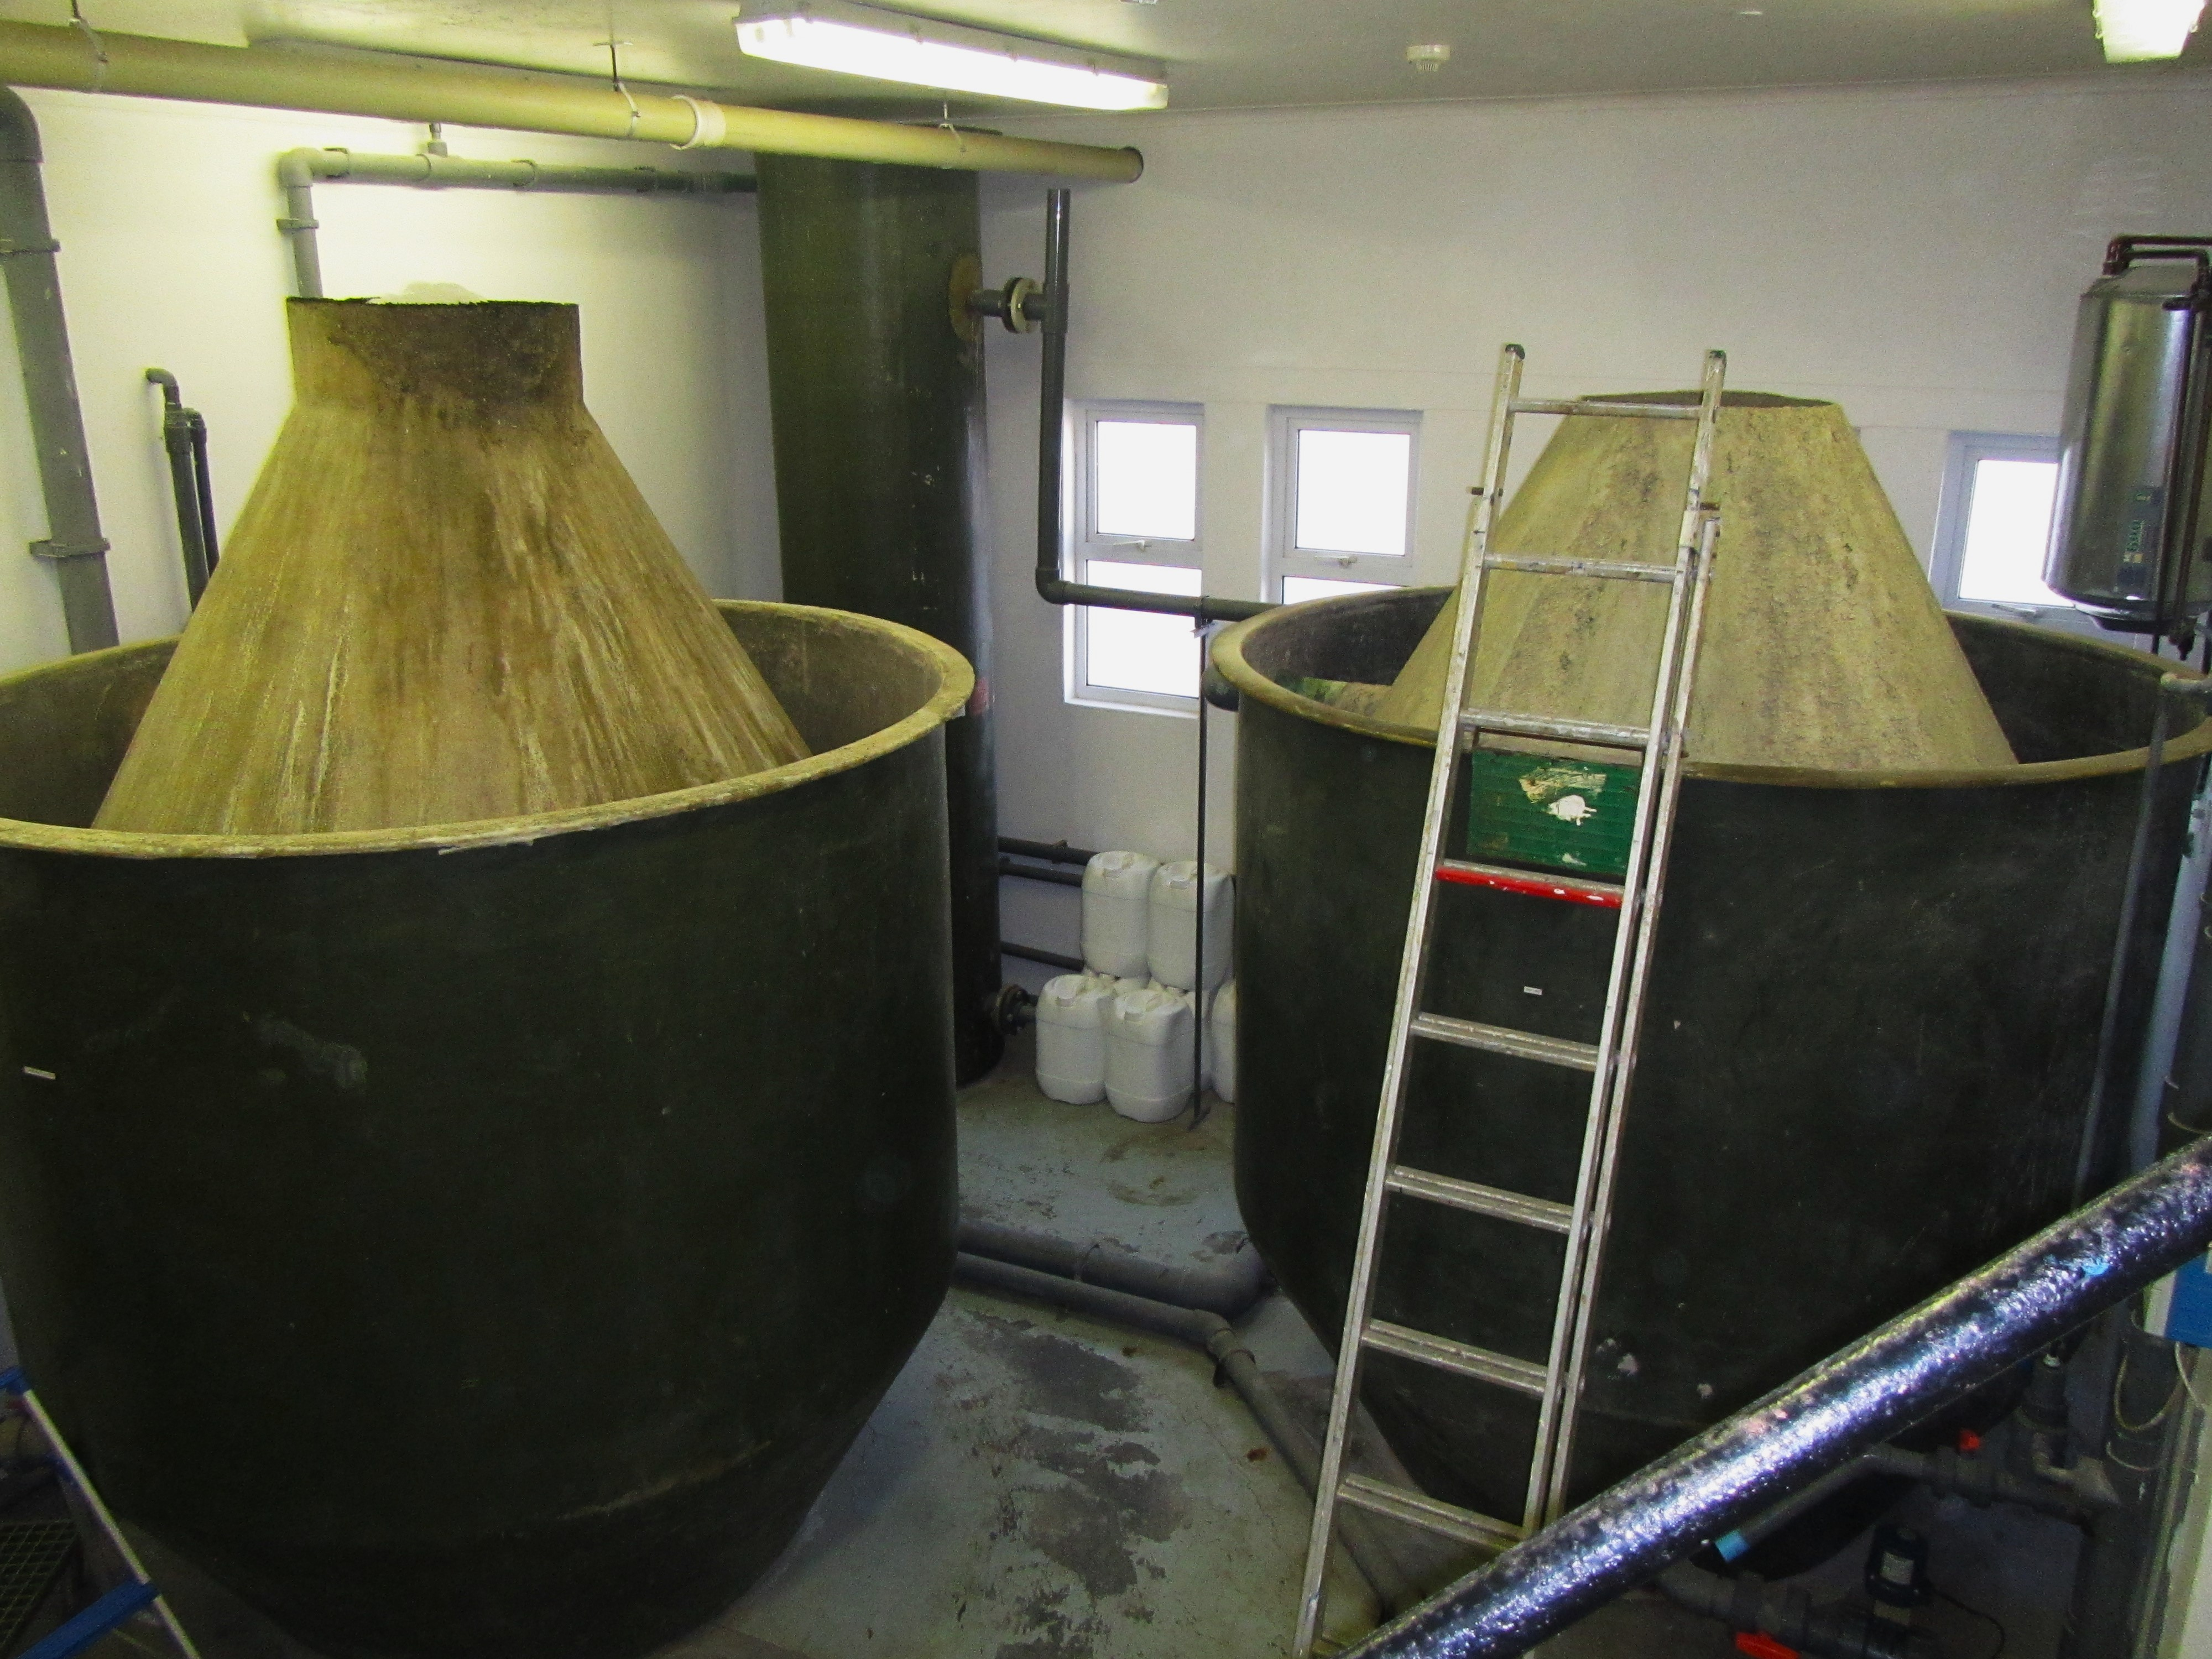
\includegraphics[width=0.5\textwidth,height=\textheight]{images/daf/biofilter.jpg}

}

\caption{\label{fig-biofilter}The Foam fractionator (left), Flocculation
column (center) and Dissolved air flotation (right) tanks.}

\end{figure}

It has one drain valve and an electric actuator valve in series with the
DAF outlet valve, along the outside of the main tank
(Figure~\ref{fig-dafcomp}). The inside of the tank consists of a smaller
central DAF column that houses a nozzle manifold connected to the
saturated water inlet pipe.

\begin{figure}[H]

\begin{minipage}[t]{0.50\linewidth}

{\centering 

\raisebox{-\height}{

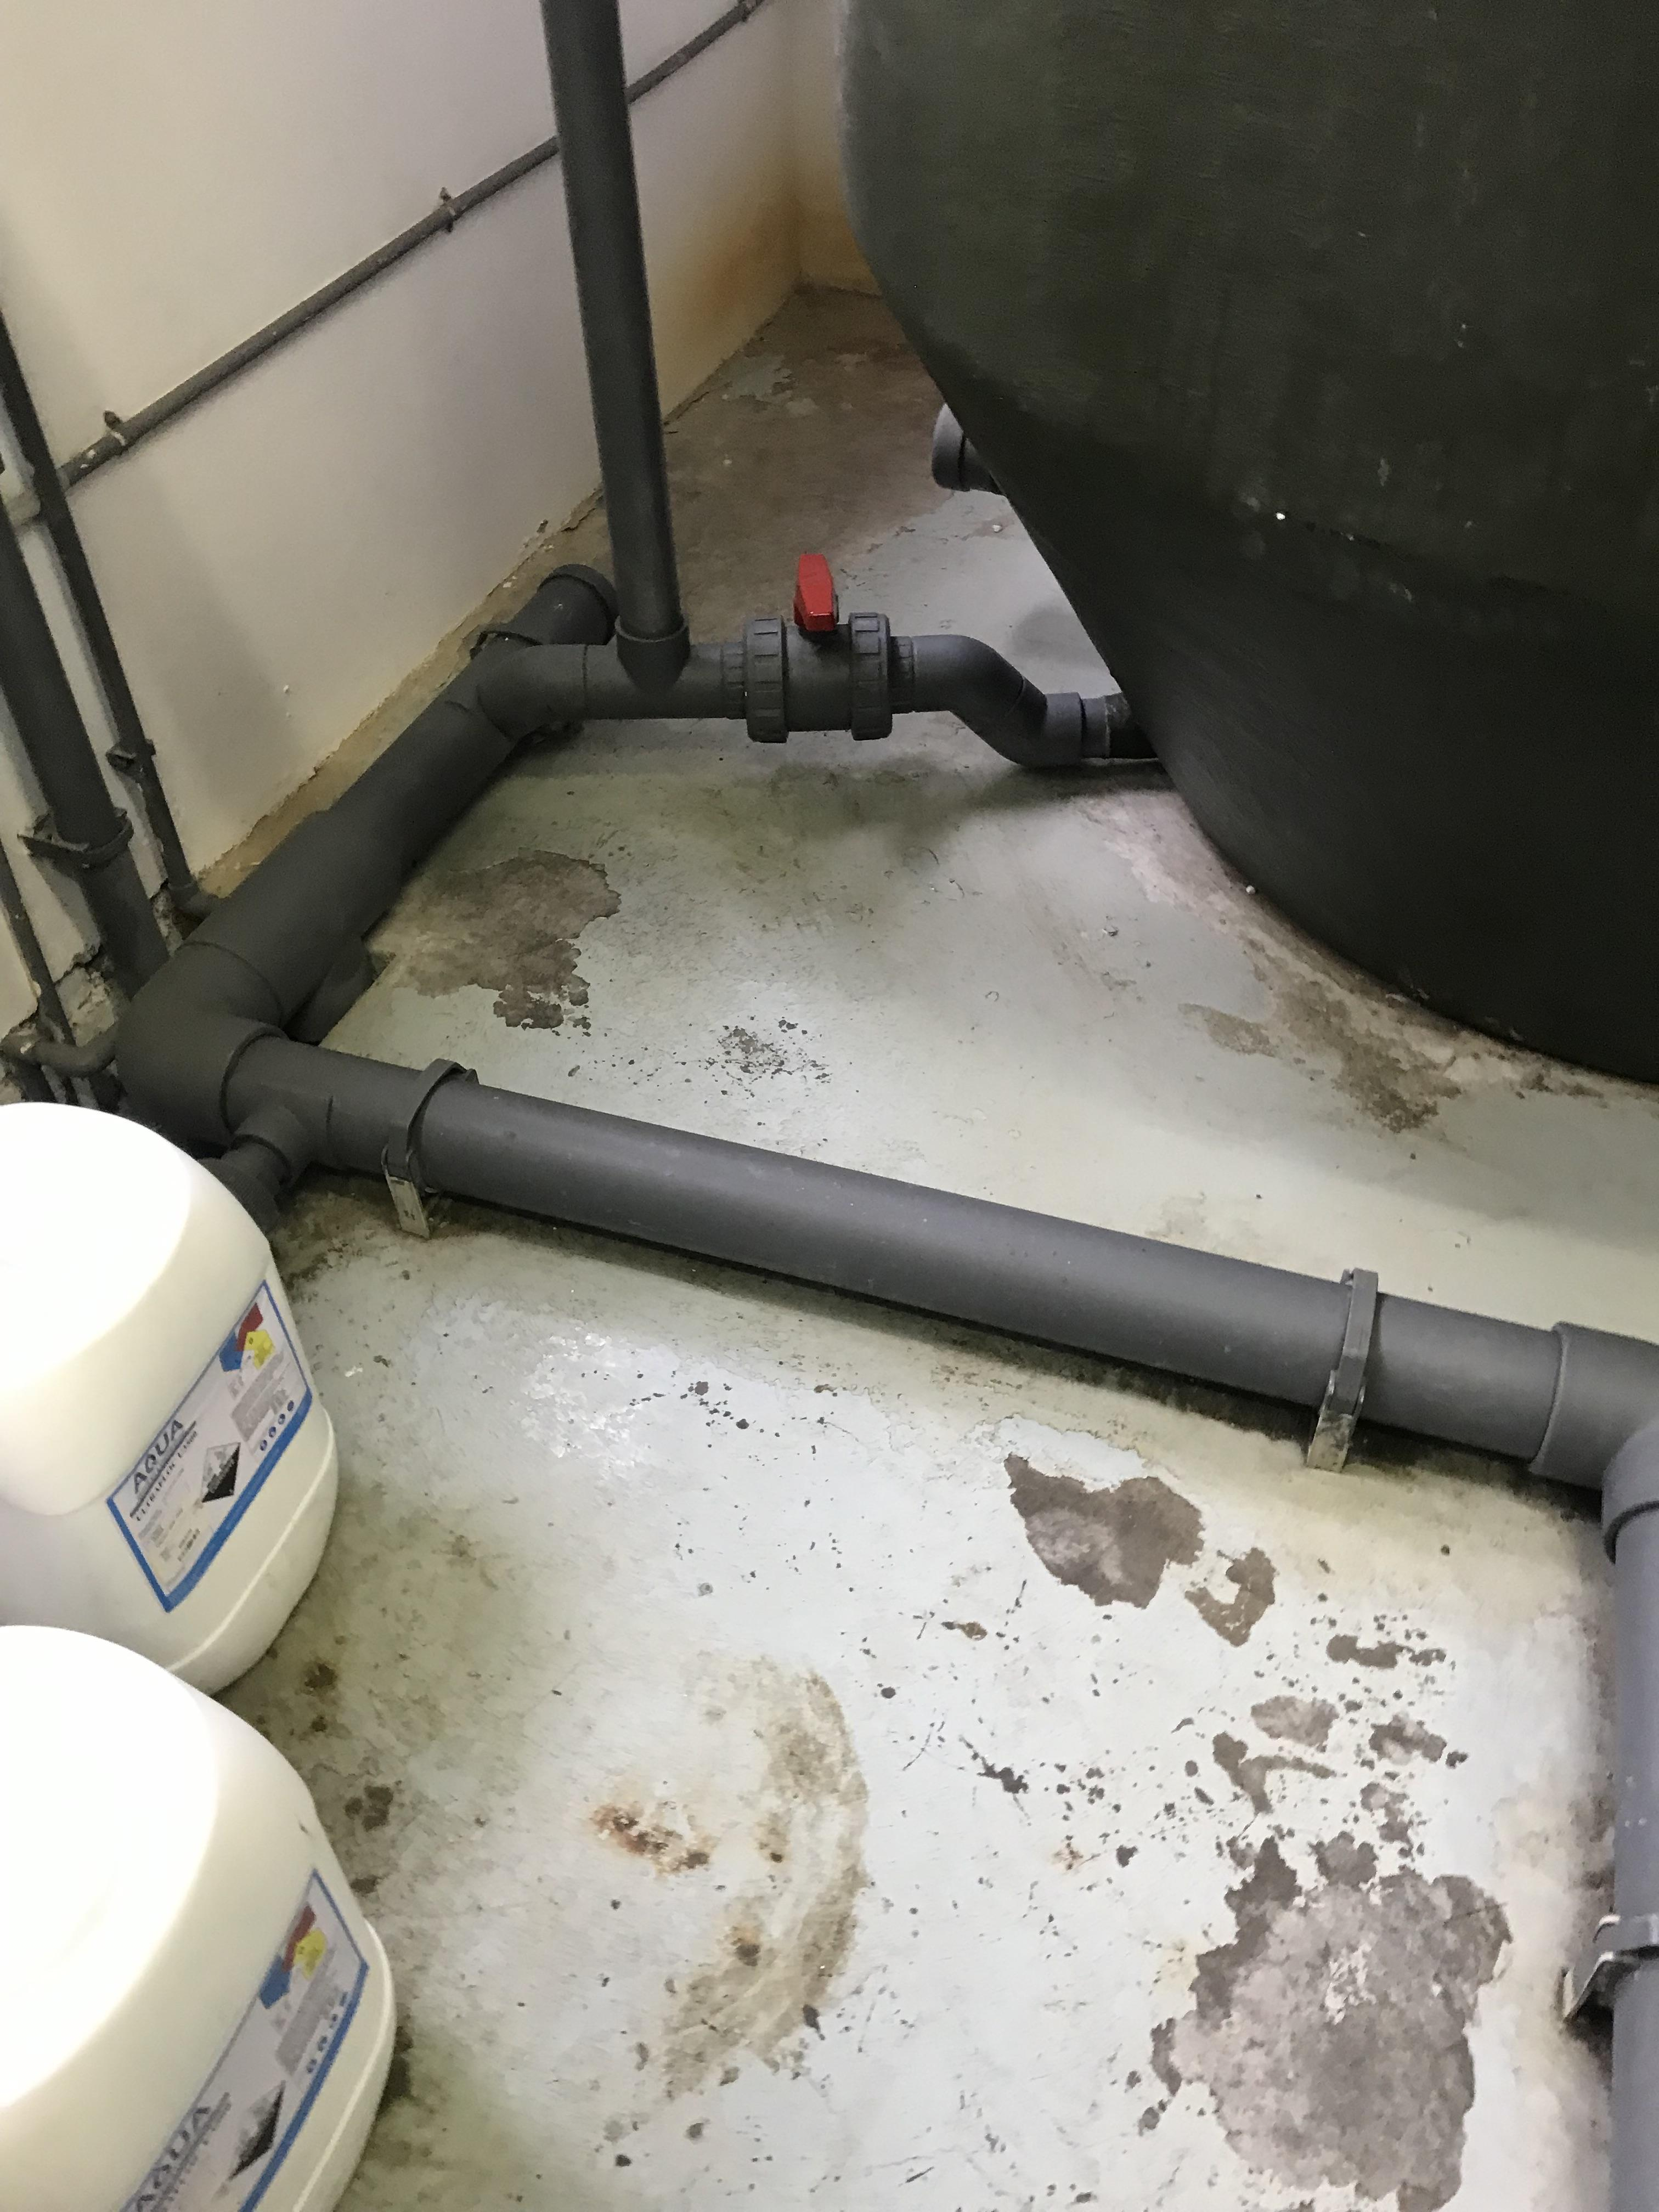
\includegraphics{images/daf/dafdrain2.jpg}

}

}

\subcaption{\label{fig-daf-drain}Drain valve}
\end{minipage}%
%
\begin{minipage}[t]{0.50\linewidth}

{\centering 

\raisebox{-\height}{

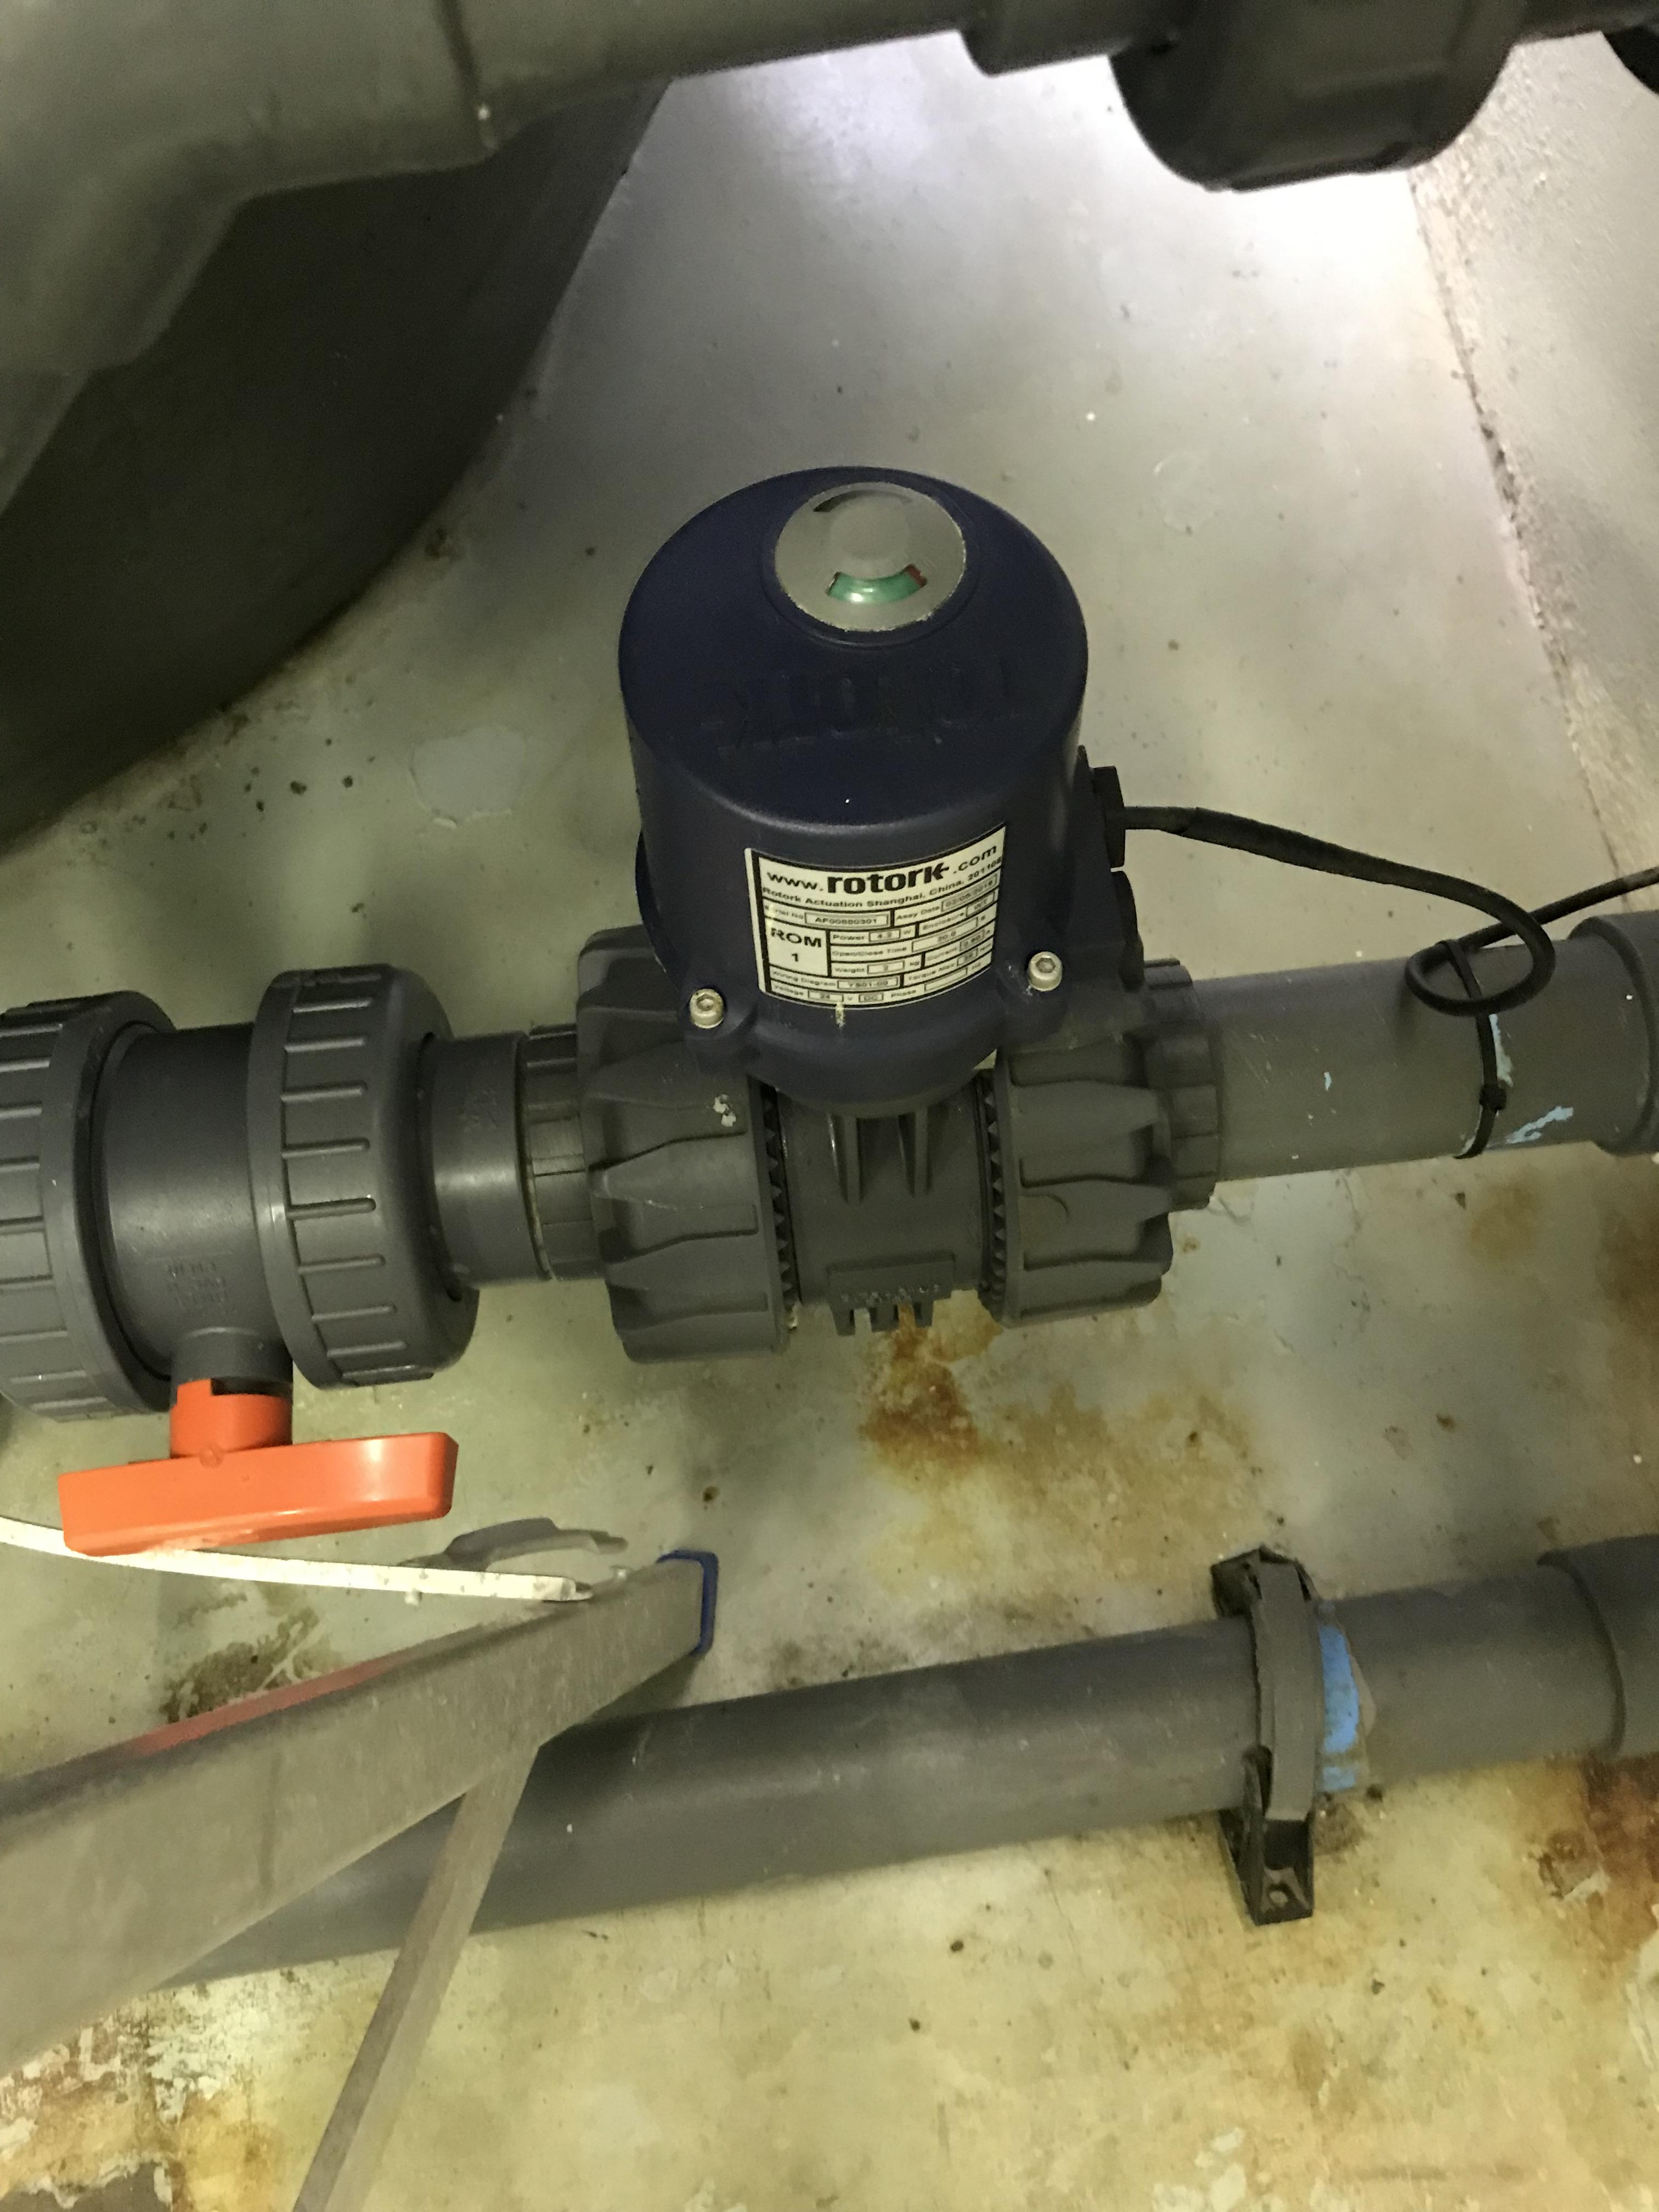
\includegraphics{images/daf/actuator2.jpg}

}

}

\subcaption{\label{fig-daf-outlet}Outlet (left) and Actuator (right)
valve}
\end{minipage}%

\caption{\label{fig-dafcomp}Image of the main components along the
outside of the DAF tank.}

\end{figure}

\hypertarget{sec-daf-maintain}{%
\section{Maintenance}\label{sec-daf-maintain}}

{The maintenance procedure described for the DAF tank should be
completed once every year}.

\hypertarget{sec-daf-tool}{%
\subsection{Tool preparation}\label{sec-daf-tool}}

\textbf{Most of the tools can be found inside the workshop (room 162)}.

These include:

\begin{itemize}
\tightlist
\item
  1 x monkey wrench
\item
  1 x long hose pipe (50mm diameter)
\item
  1 x Ladder (approximately 1.8m long)
\item
  1 x long stick (approximately 2.2m long)
\item
  2 x Fish scoop nets
\item
  1 x Bucket
\end{itemize}

\textbf{To conduct annual maintenance, the DAF tank has to be drained
completely}.

\hypertarget{drain-daf}{%
\subsection{Drain DAF}\label{drain-daf}}

\begin{itemize}
\tightlist
\item
  \textbf{Steps 1-6 will be completed inside the plant room}.
\end{itemize}

\begin{enumerate}
\def\labelenumi{\arabic{enumi}.}
\tightlist
\item
  Close Dump valve No.~18 (Figure~\ref{fig-dump-valve}).
\item
  Wait for the water level at the Prosonic HMU 860 to reach 90\%
  (Figure~\ref{fig-prosonic}).

  \begin{itemize}
  \tightlist
  \item
    \emph{Done to ensure enough sea water remains in circulation during
    the maintenance procedure}.
  \end{itemize}
\item
  Switch off the Jetty pump on the Main control switchboard
  (Figure~\ref{fig-mcs}).

  \begin{itemize}
  \tightlist
  \item
    \emph{Prevents more water intake}.
  \end{itemize}
\end{enumerate}

\begin{figure}[H]

\begin{minipage}[t]{0.33\linewidth}

{\centering 

\raisebox{-\height}{

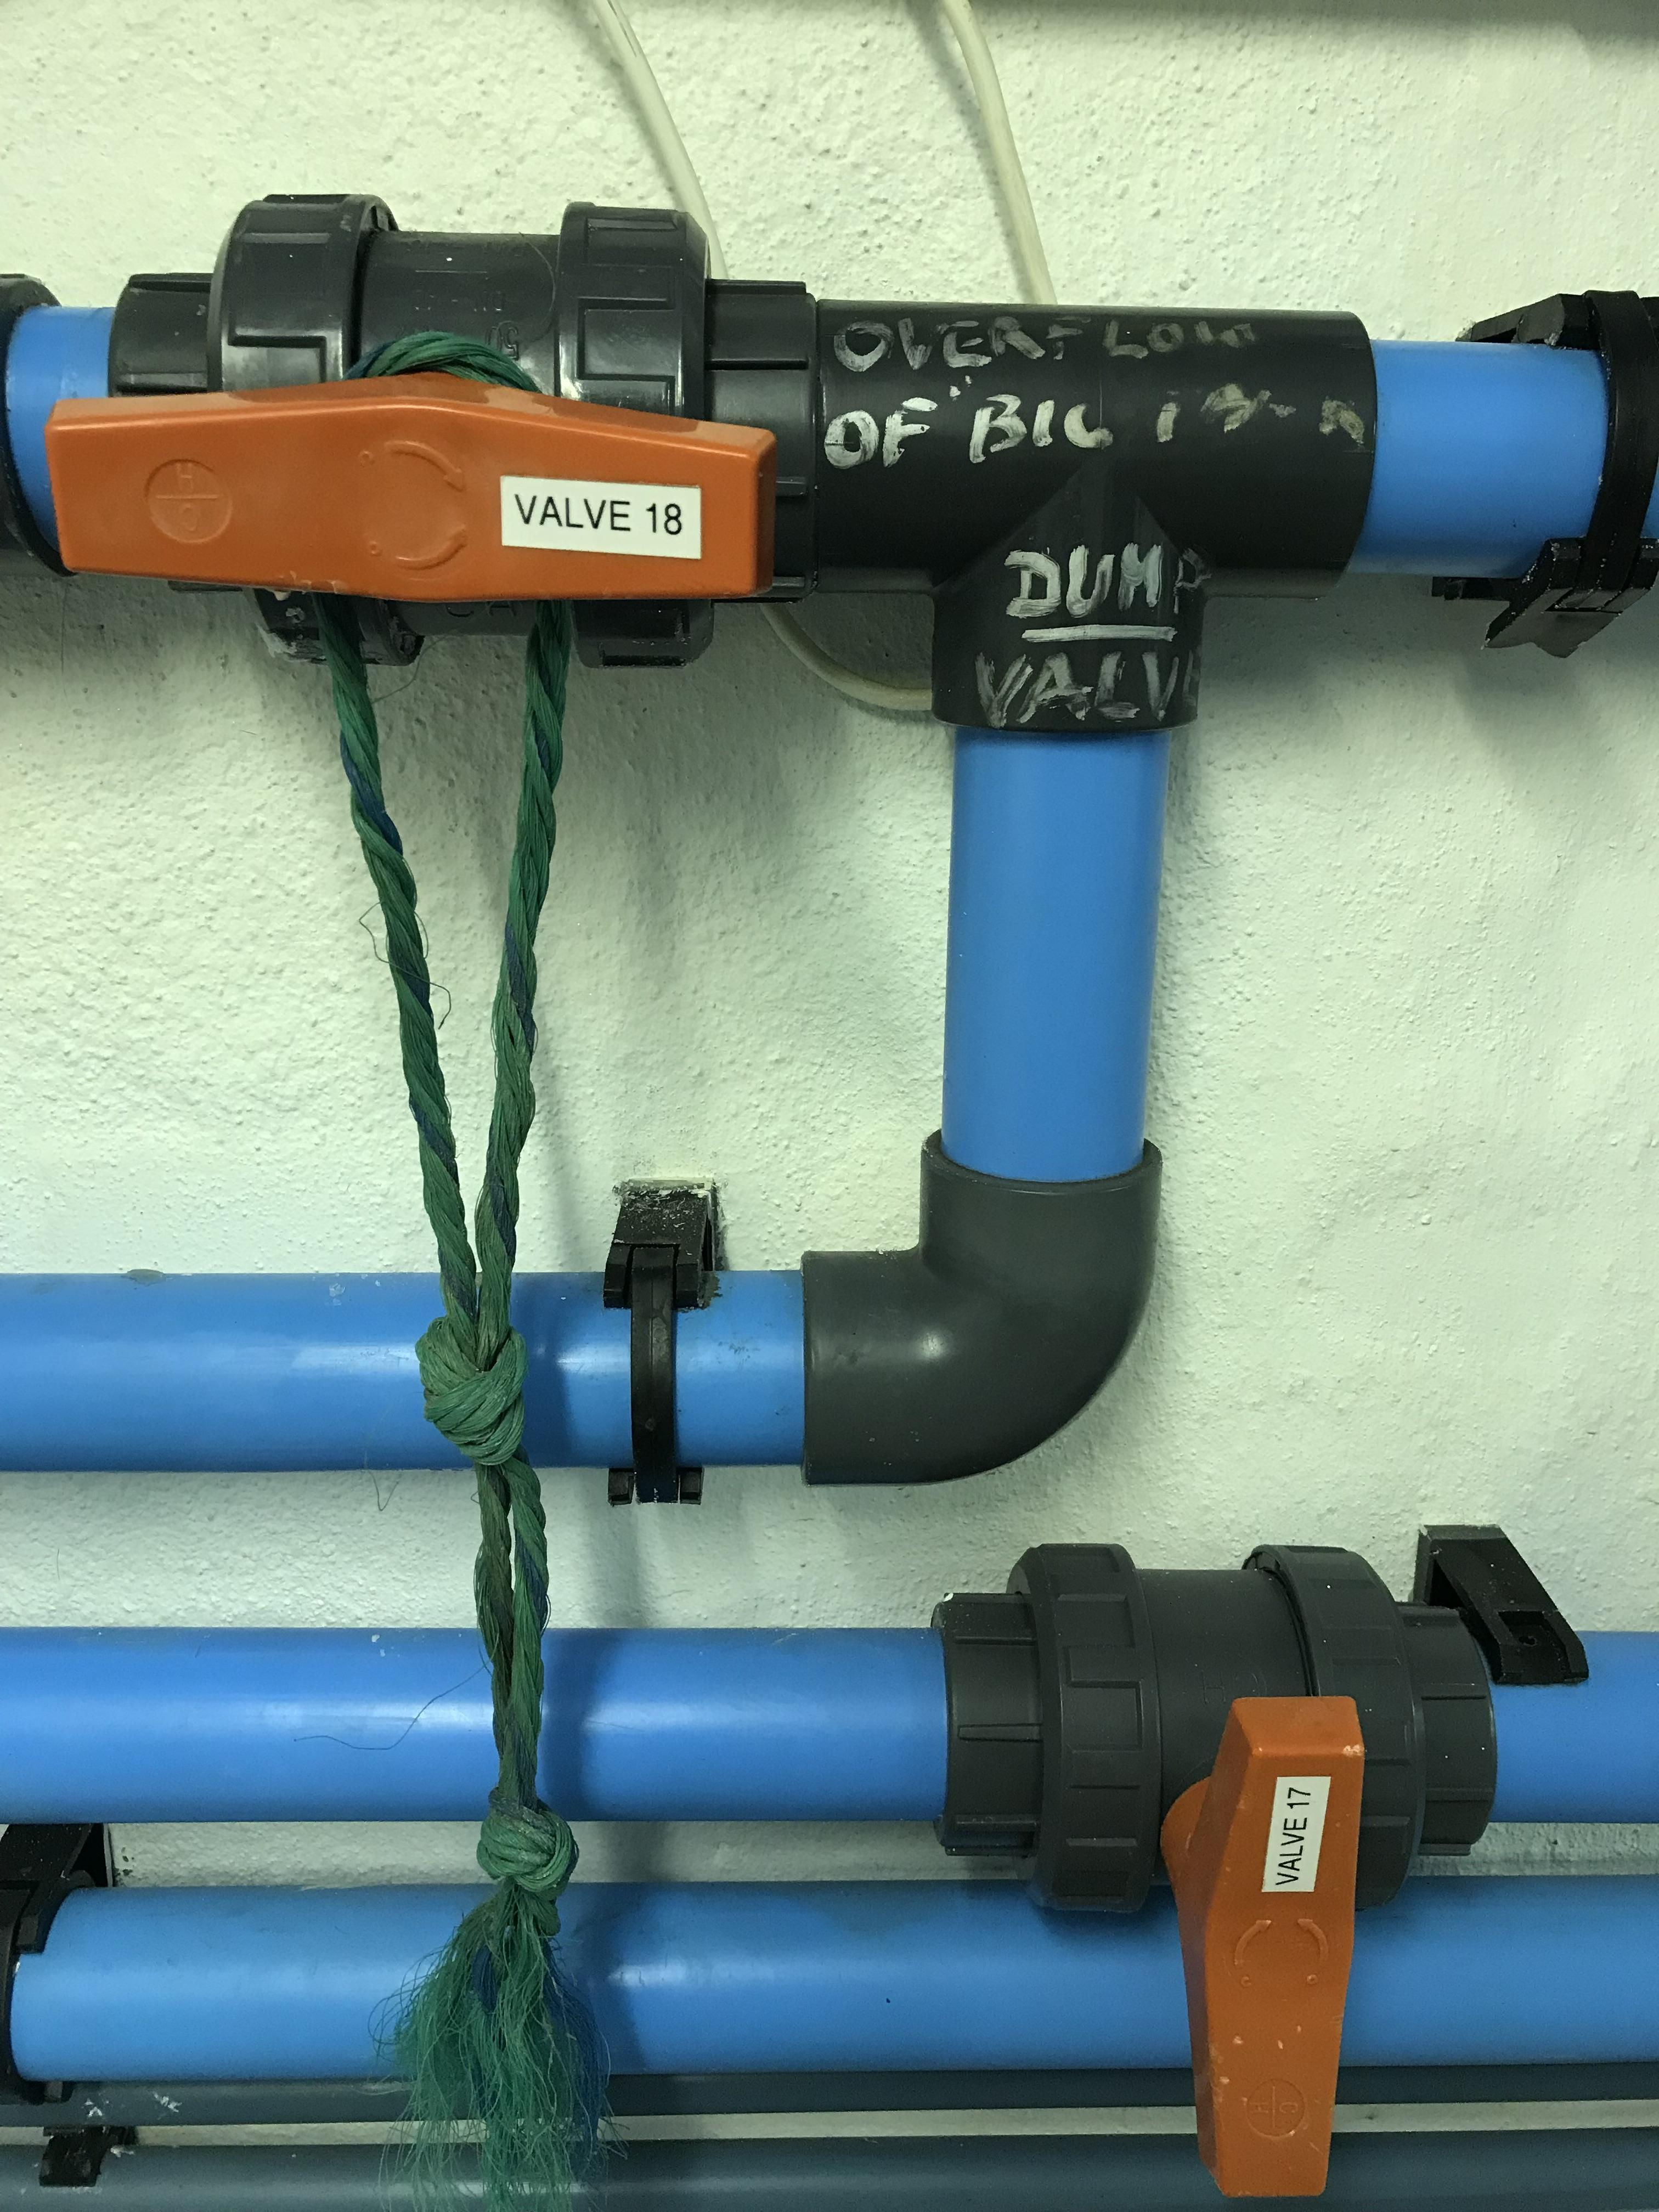
\includegraphics{images/plant_room/dump_valve2.jpg}

}

}

\subcaption{\label{fig-dump-valve}Dump valve}
\end{minipage}%
%
\begin{minipage}[t]{0.33\linewidth}

{\centering 

\raisebox{-\height}{

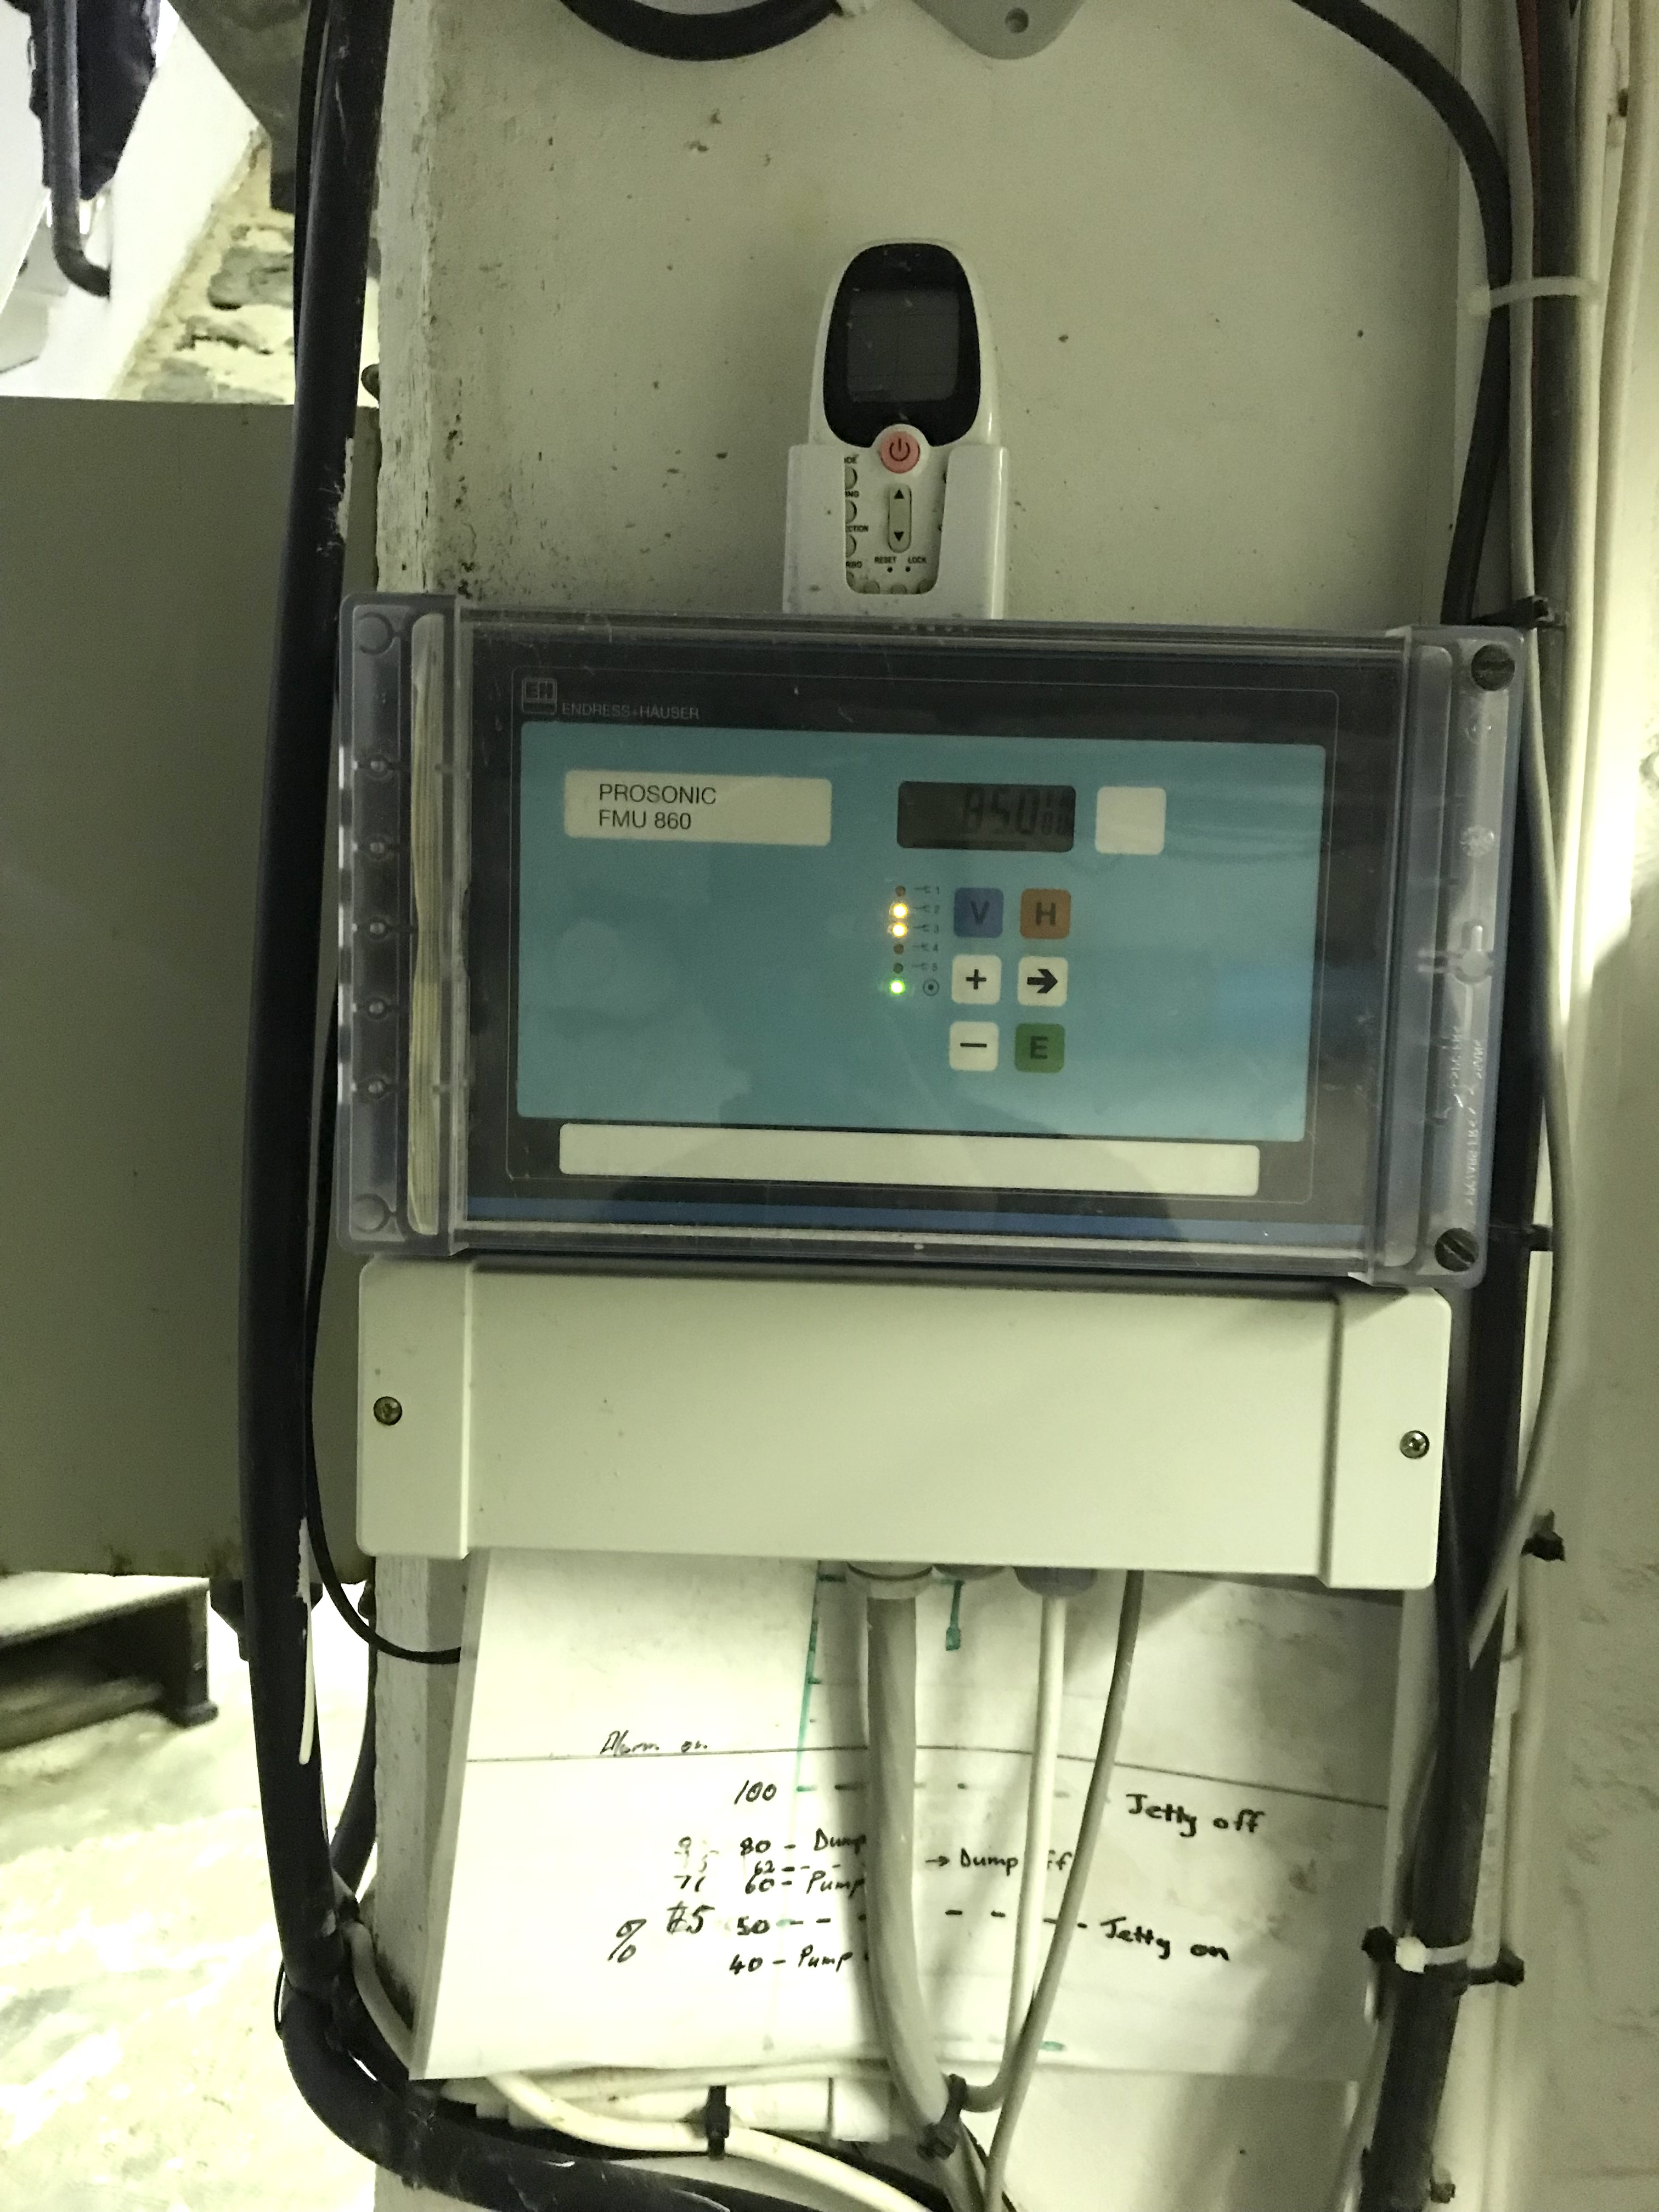
\includegraphics{images/plant_room/prosonic.jpg}

}

}

\subcaption{\label{fig-prosonic}Prosonic HMU 860}
\end{minipage}%
%
\begin{minipage}[t]{0.33\linewidth}

{\centering 

\raisebox{-\height}{

\includegraphics{images/plant_room/main_switch2.jpg}

}

}

\subcaption{\label{fig-mcs}Main control switchboard}
\end{minipage}%

\caption{\label{fig-seacirc}Some of the components needed to control the
circulation of water and air between the Aquarium and the sea, and
within the Aquarium.}

\end{figure}

\begin{enumerate}
\def\labelenumi{\arabic{enumi}.}
\setcounter{enumi}{3}
\tightlist
\item
  Switch off the Saturator pump.

  \begin{itemize}
  \tightlist
  \item
    \emph{Clipsal power outlet No.~2} (Figure~\ref{fig-sat-power}).
  \end{itemize}
\item
  Close the Saturator isolating valve No.~36
  (Figure~\ref{fig-sat-inlet}).

  \begin{itemize}
  \tightlist
  \item
    \emph{Feeds the Saturator system}.
  \end{itemize}
\item
  Close the Saturator discharge valve (No.~42) to the DAF tank
  (Figure~\ref{fig-sat-outlet}).
\end{enumerate}

\begin{itemize}
\tightlist
\item
  \textbf{Steps 3 - 6 prevent water flow into the DAF unit during the
  maintenance procedure}.
\end{itemize}

\begin{figure}[H]

\begin{minipage}[t]{0.50\linewidth}

{\centering 

\raisebox{-\height}{

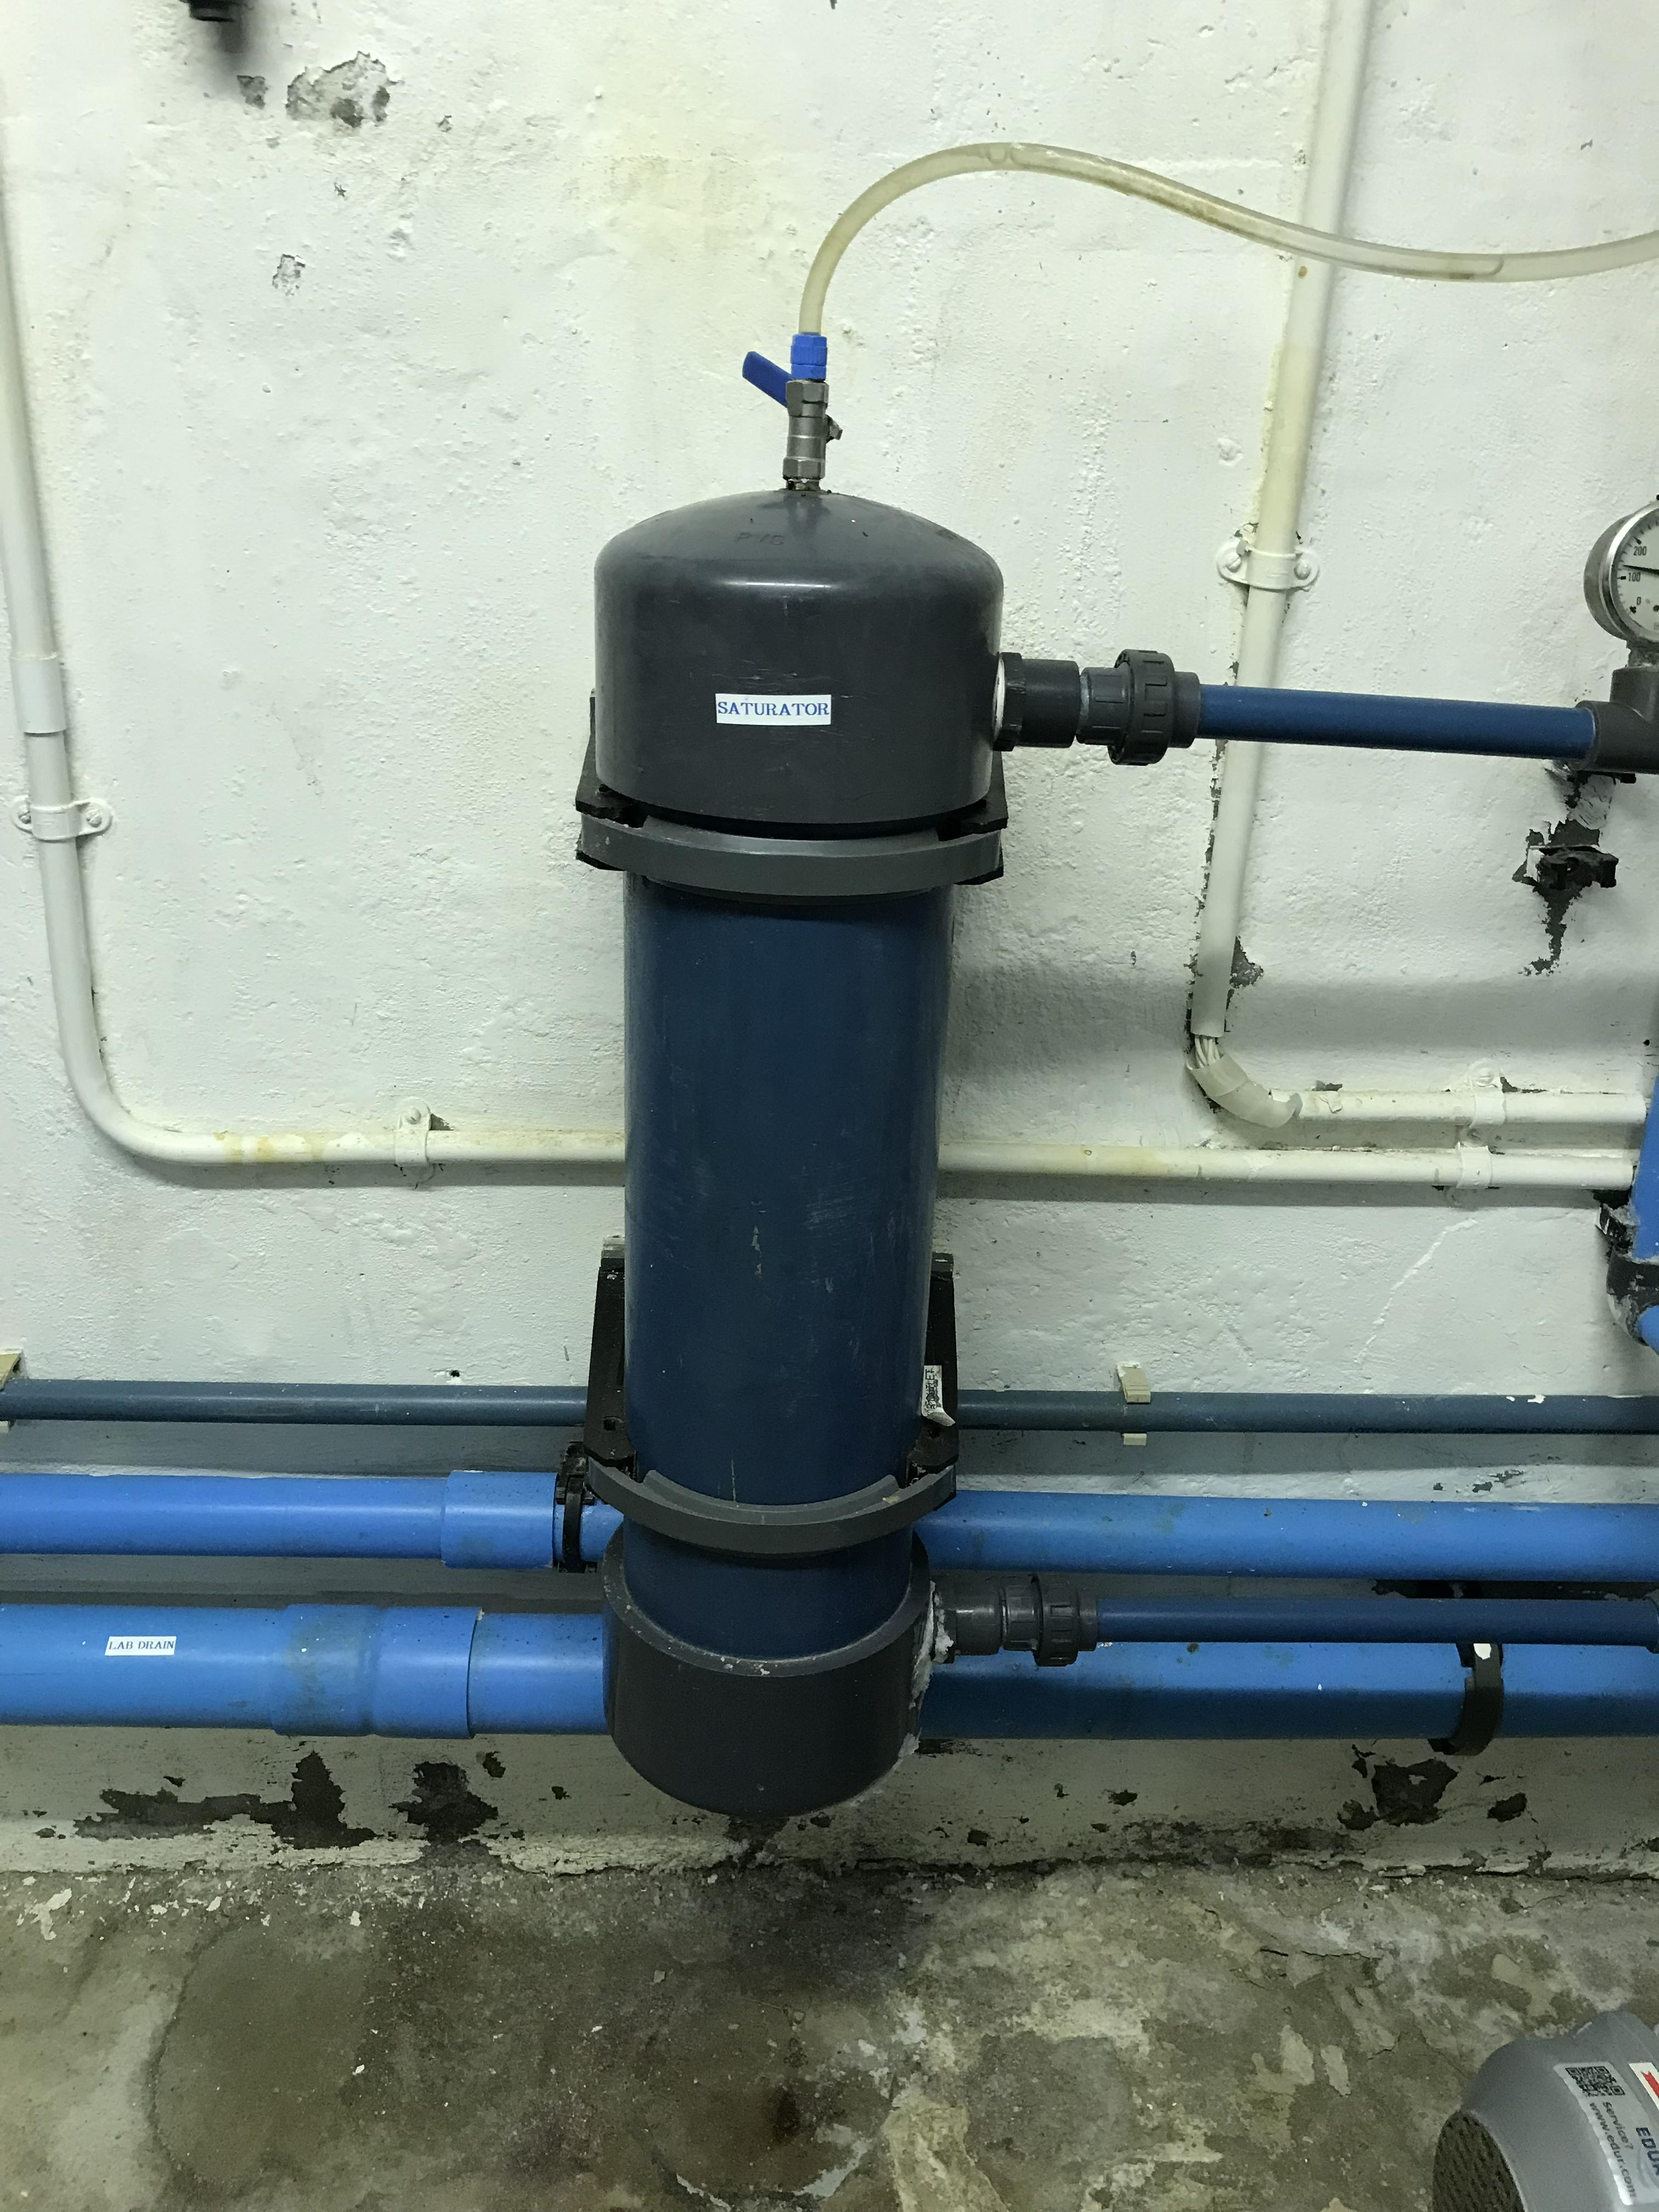
\includegraphics{images/plant_room/saturator2.jpg}

}

}

\subcaption{\label{fig-sat}Saturator}
\end{minipage}%
%
\begin{minipage}[t]{0.50\linewidth}

{\centering 

\raisebox{-\height}{

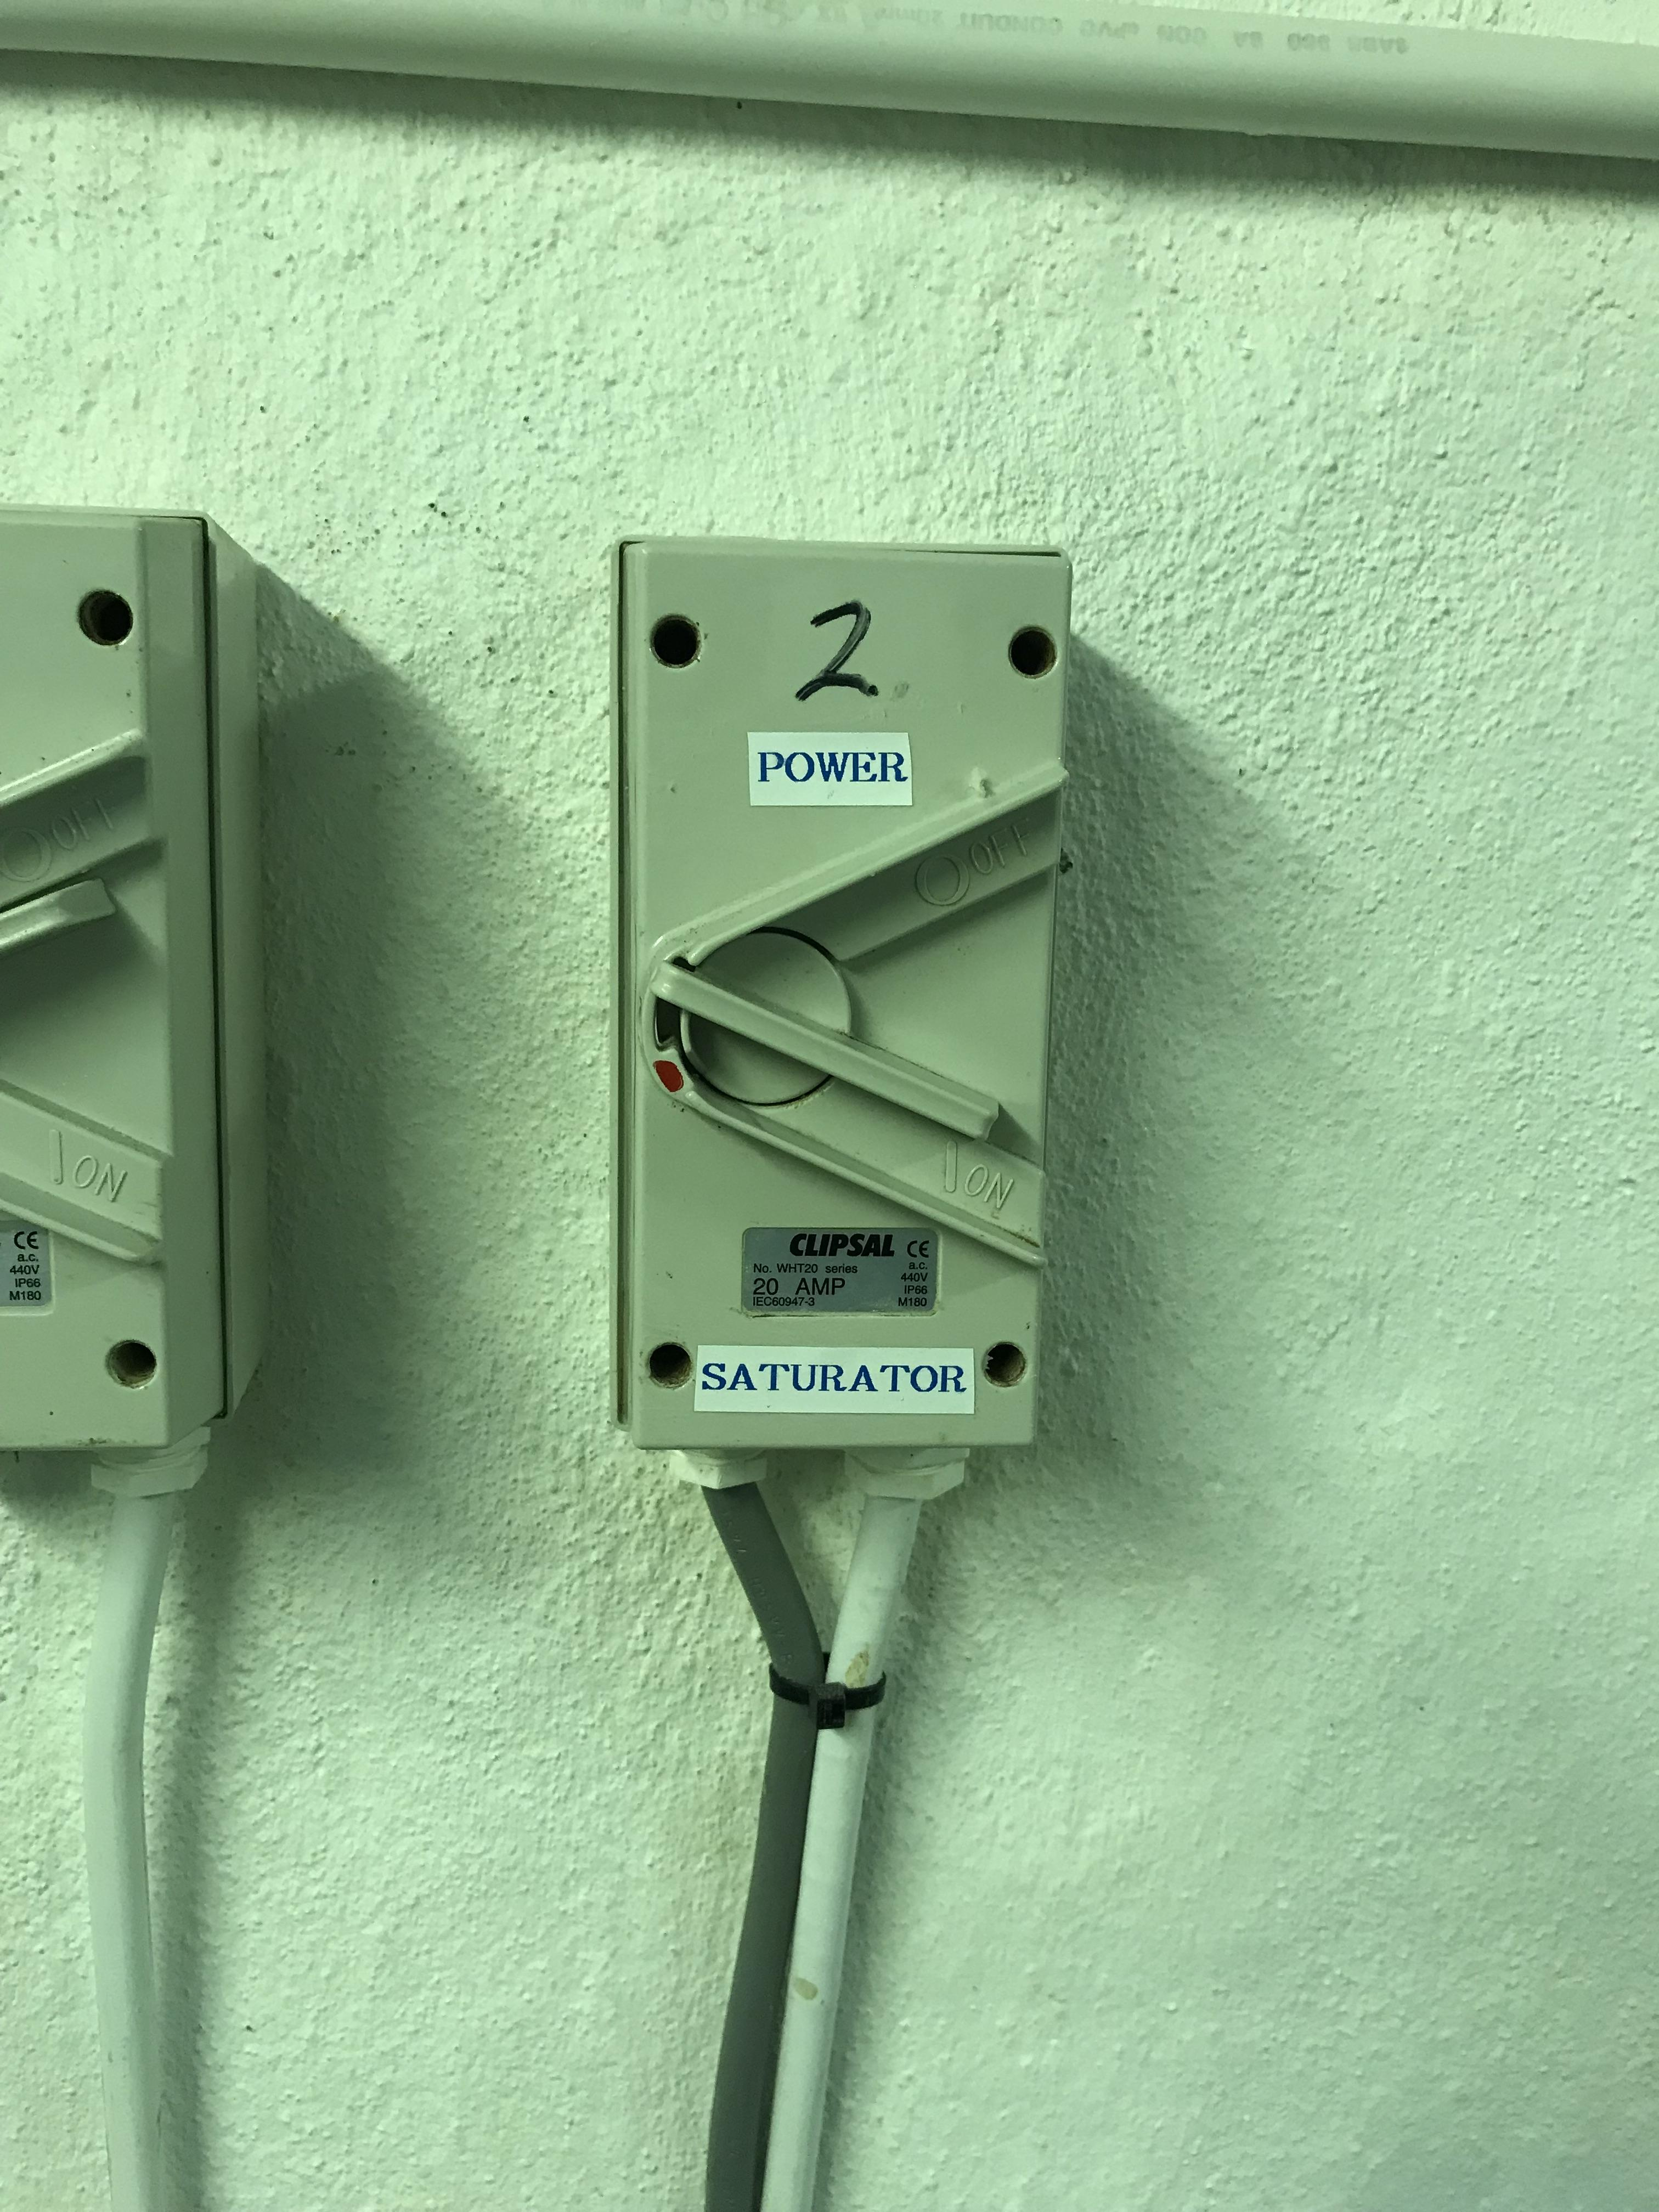
\includegraphics{images/plant_room/saturator_power2.jpg}

}

}

\subcaption{\label{fig-sat-power}Saturator power outlet}
\end{minipage}%
\newline
\begin{minipage}[t]{0.50\linewidth}

{\centering 

\raisebox{-\height}{

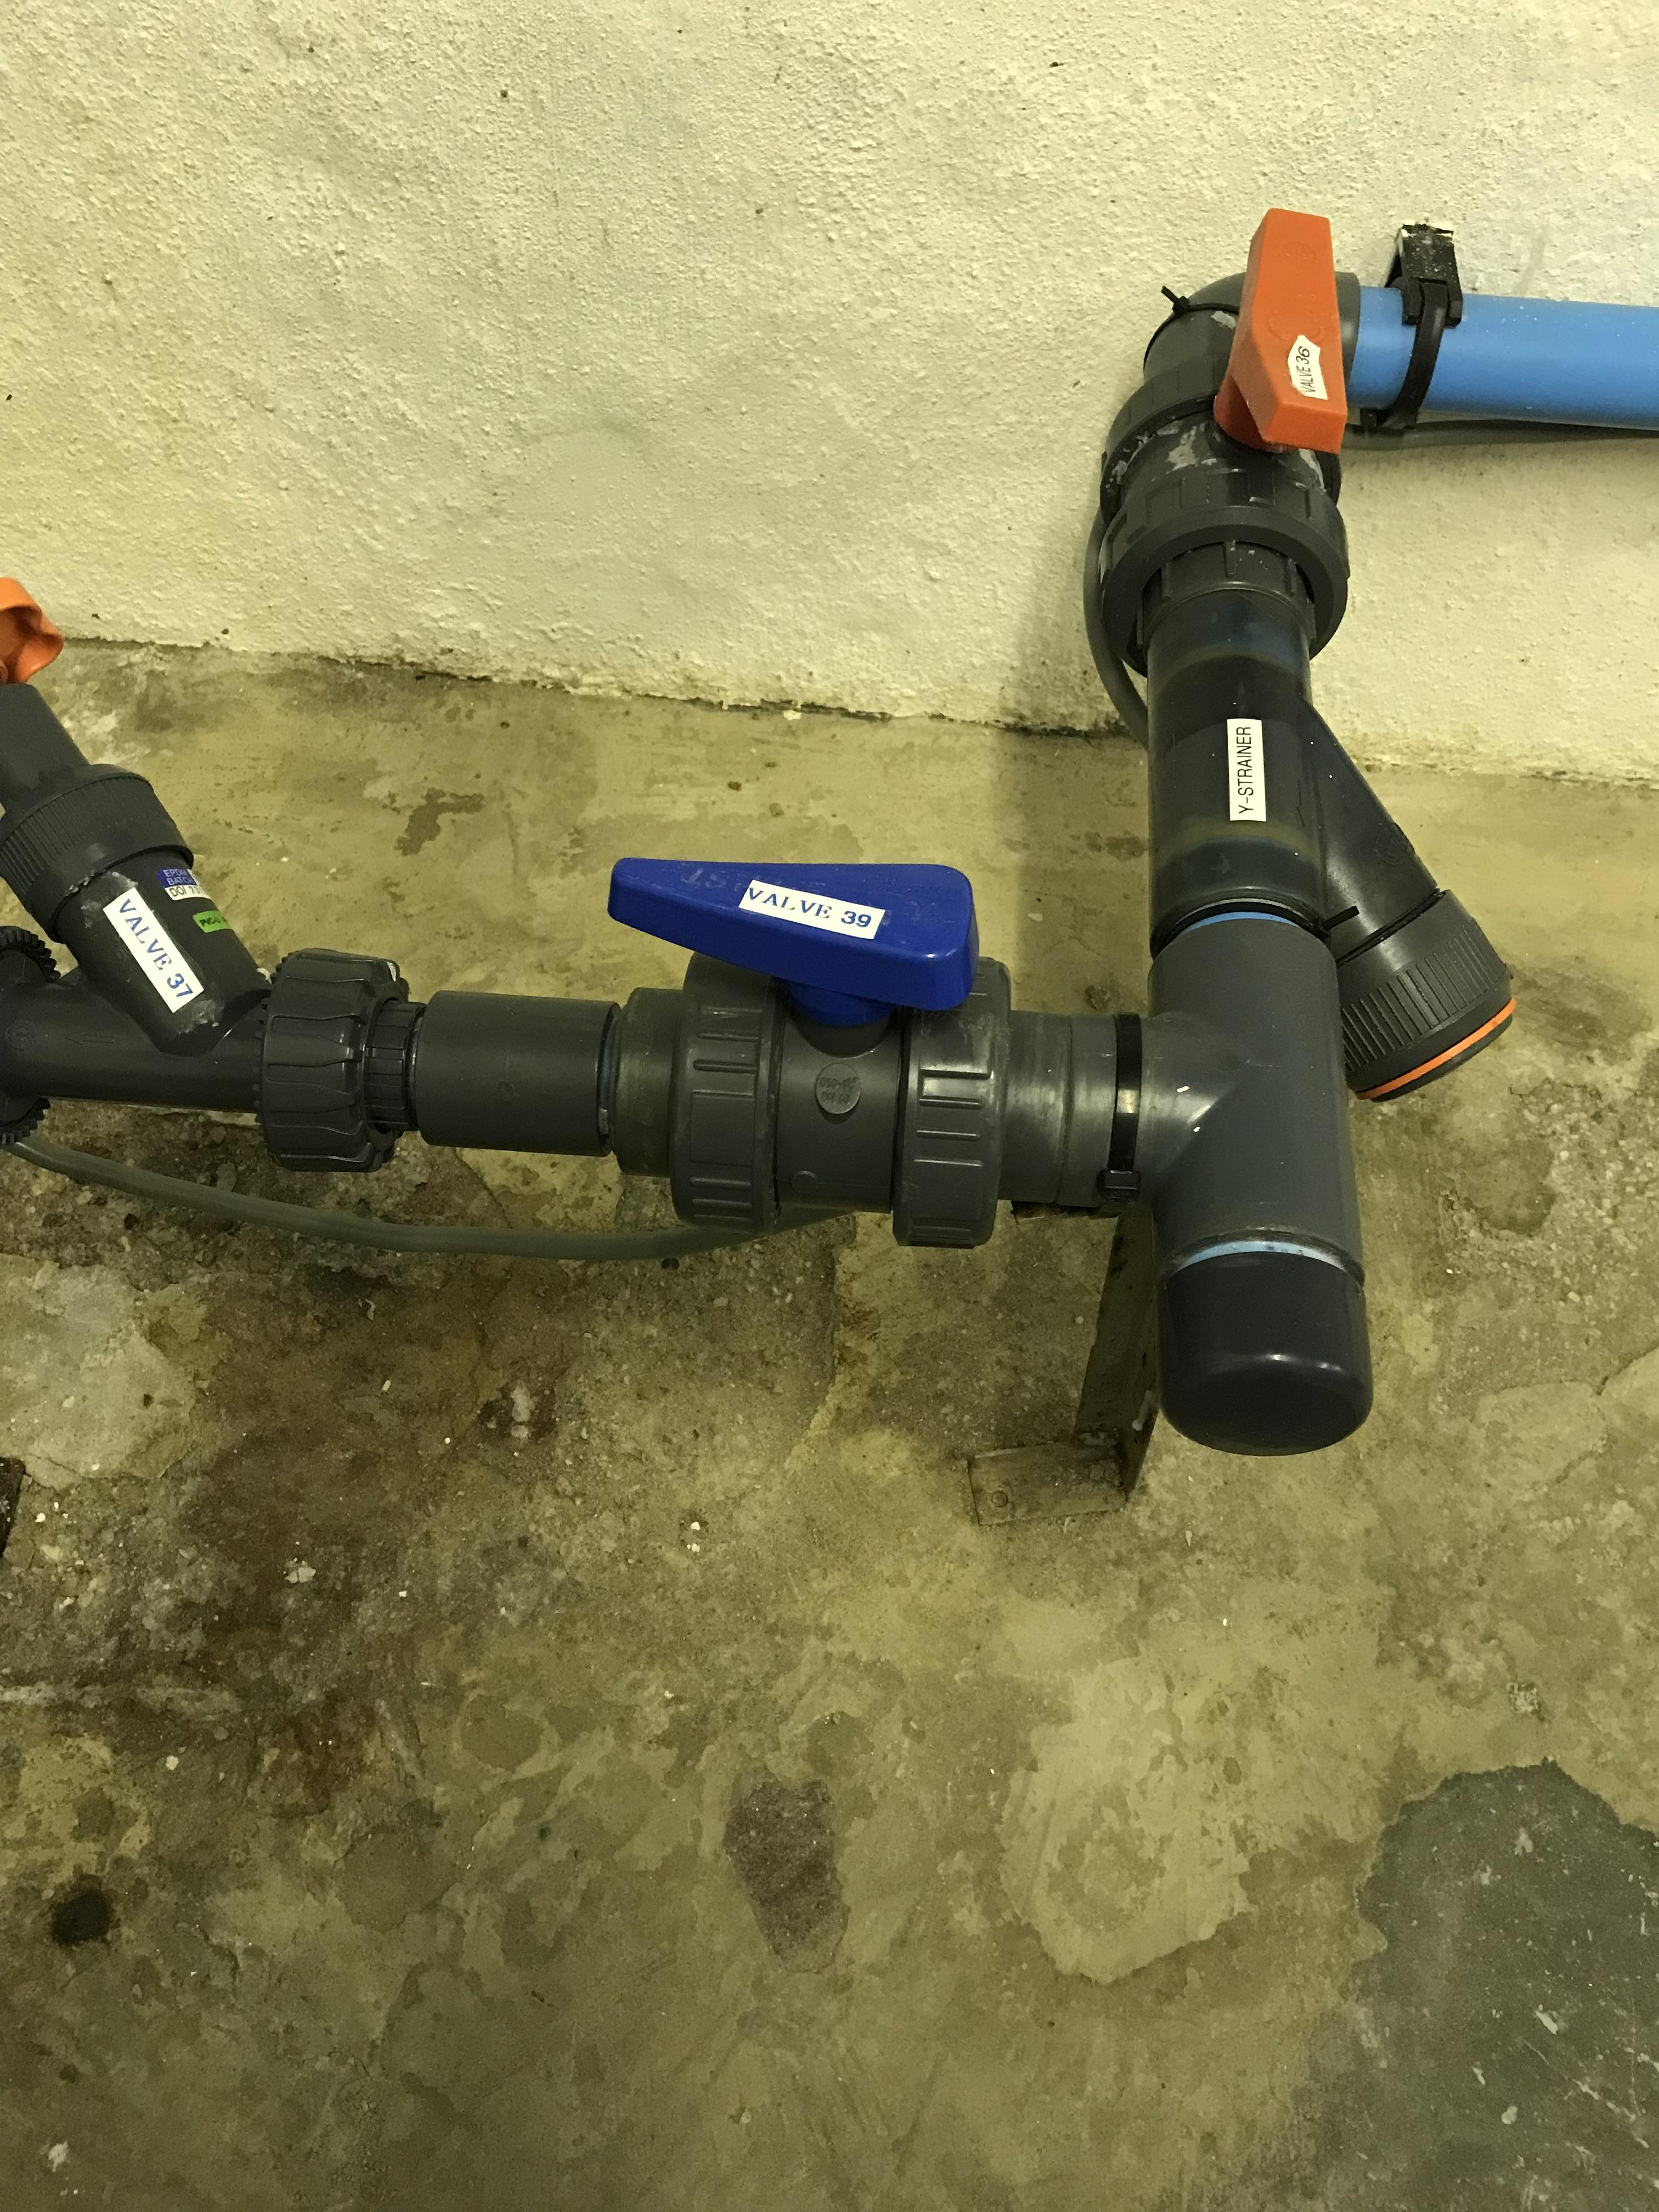
\includegraphics{images/plant_room/saturator_isolating2.jpg}

}

}

\subcaption{\label{fig-sat-inlet}Saturator inlet valve.}
\end{minipage}%
%
\begin{minipage}[t]{0.50\linewidth}

{\centering 

\raisebox{-\height}{

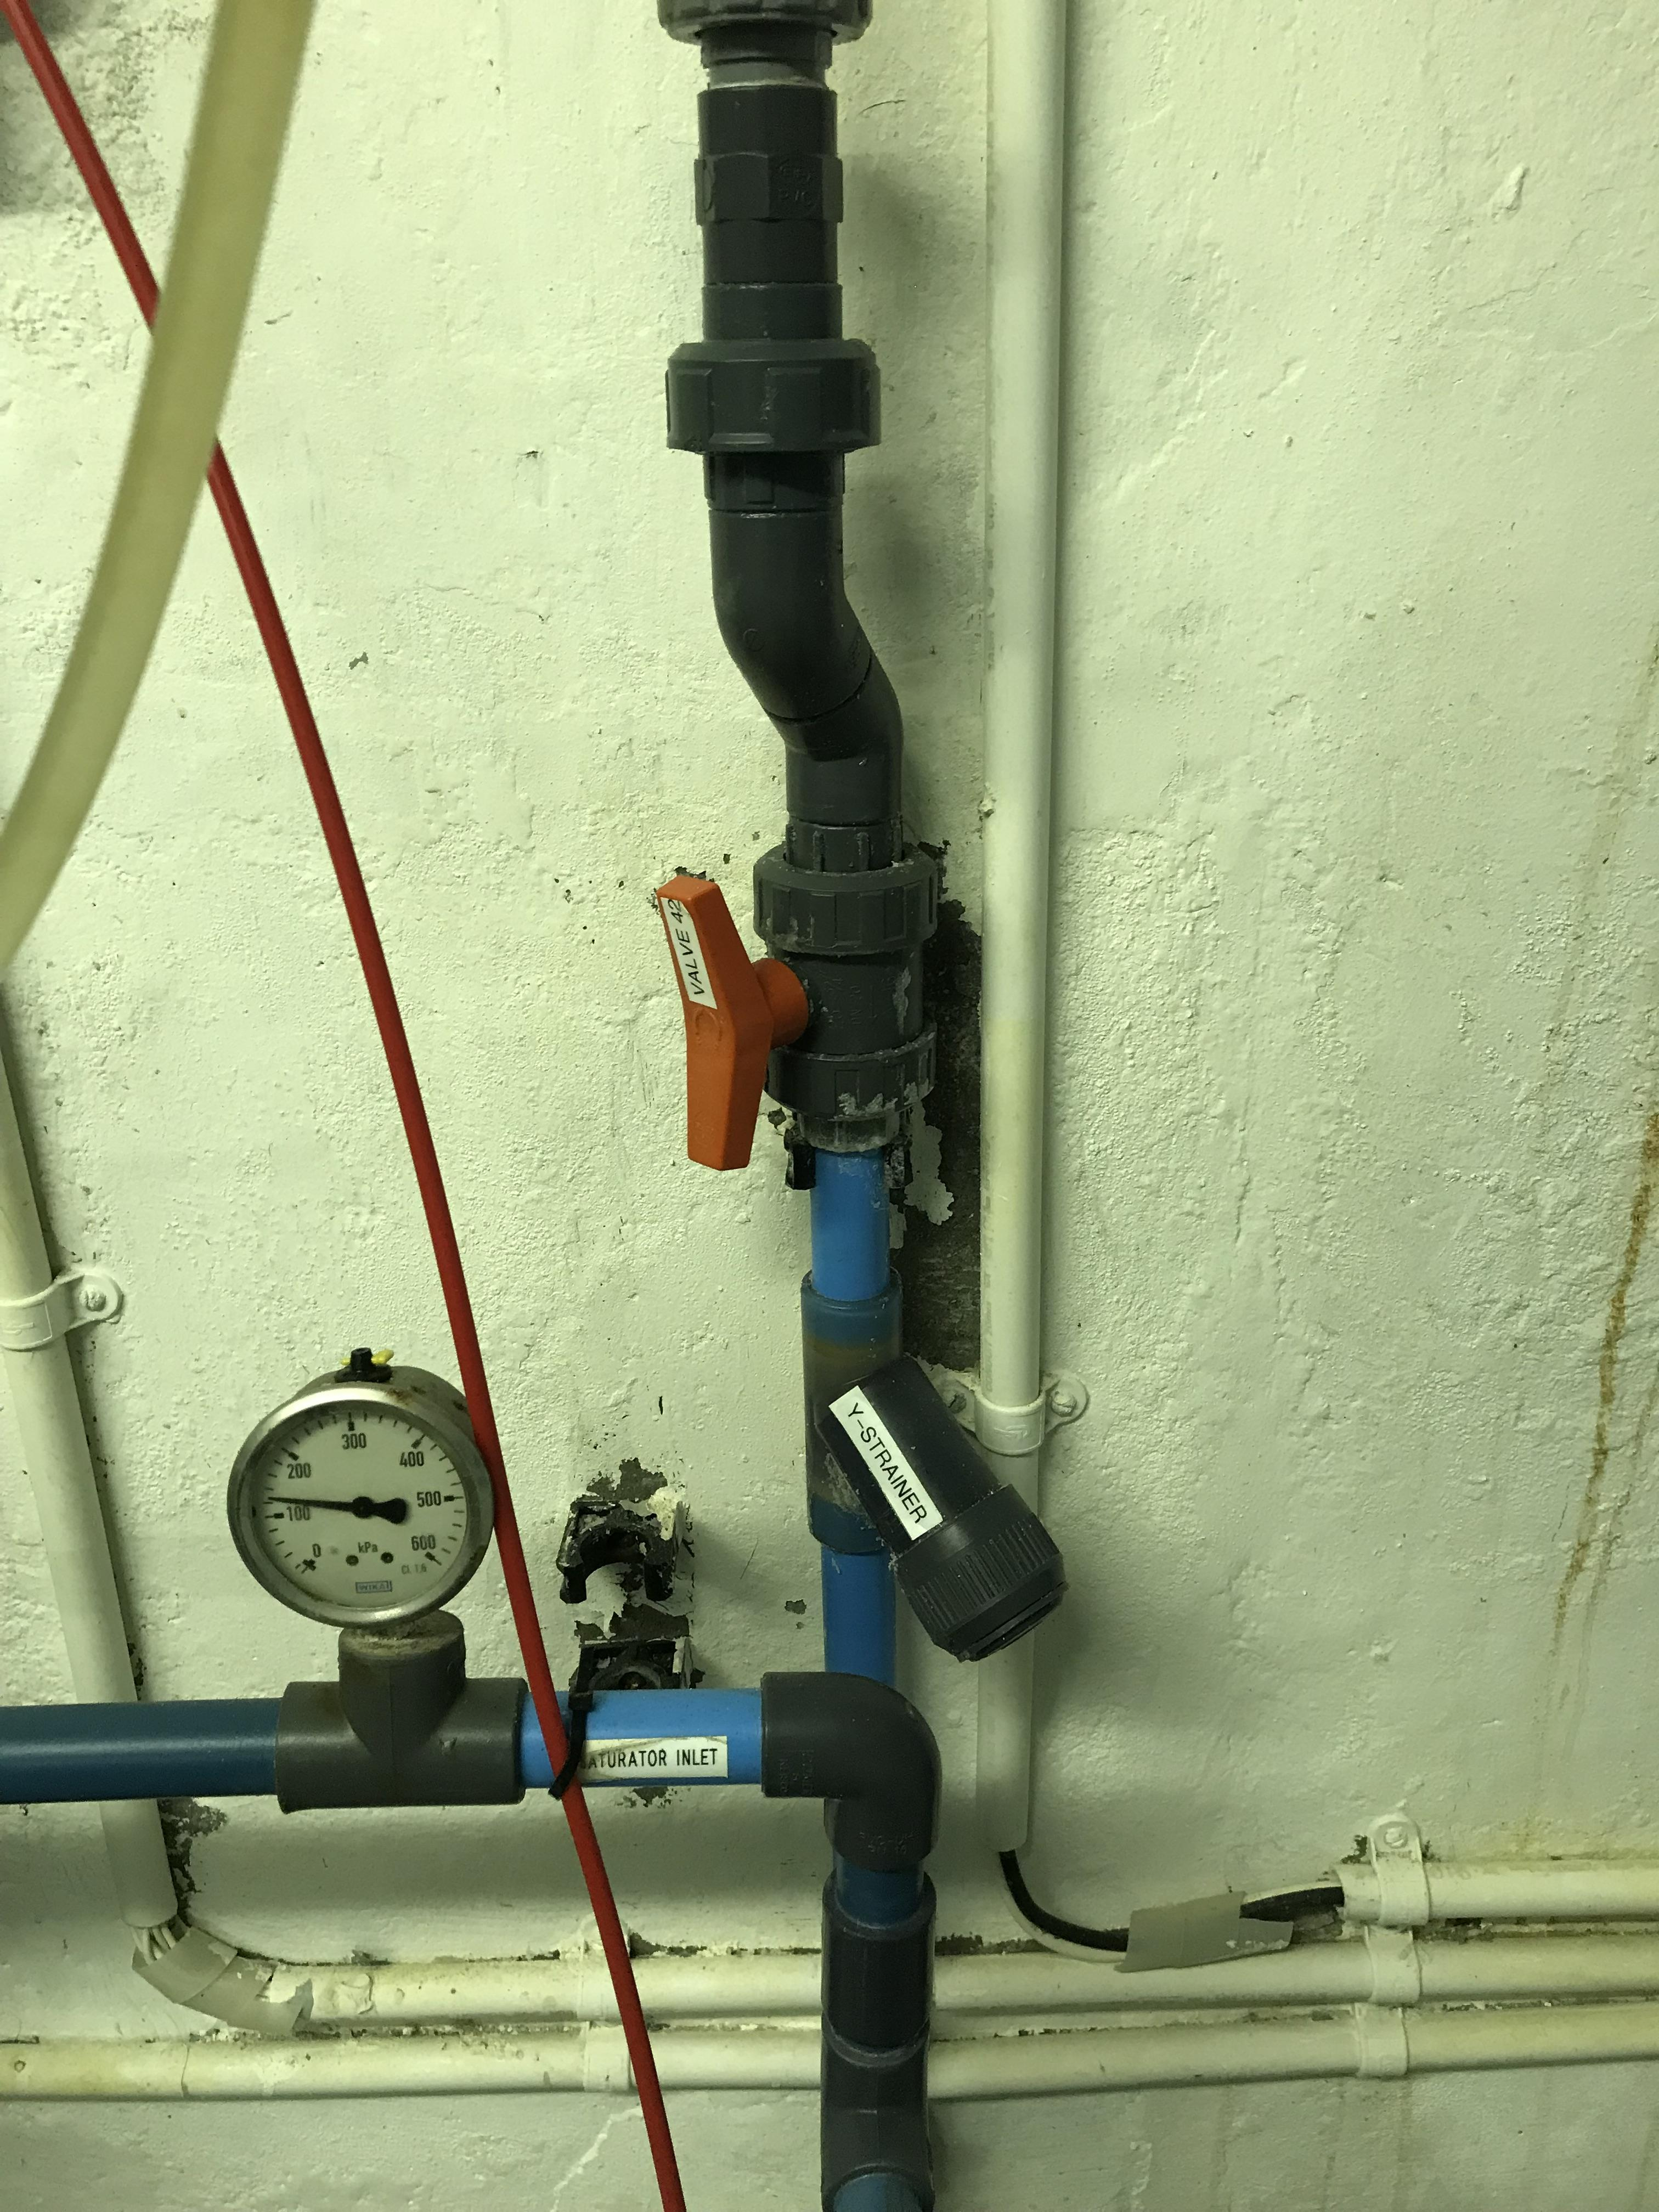
\includegraphics{images/plant_room/saturator_discharge2.jpg}

}

}

\subcaption{\label{fig-sat-outlet}Saturator outlet valve.}
\end{minipage}%

\caption{\label{fig-sat-comp}The saturator and all the components
required to control water flow from the saturator into the DAF unit.}

\end{figure}

\begin{enumerate}
\def\labelenumi{\arabic{enumi}.}
\setcounter{enumi}{6}
\tightlist
\item
  Open DAF drain valve (No.~43).
\item
  Allow DAF to drain completely.
\end{enumerate}

\begin{itemize}
\tightlist
\item
  \textbf{Some water still remains in central DAF column after
  draining}.
\end{itemize}

\hypertarget{inspect-nozzle-manifold-and-associated-parts}{%
\subsection{Inspect Nozzle manifold and associated
parts}\label{inspect-nozzle-manifold-and-associated-parts}}

{This is a job for a minimum of 2 people}.

\begin{enumerate}
\def\labelenumi{\arabic{enumi}.}
\setcounter{enumi}{8}
\tightlist
\item
  Uncouple the Nozzle manifold from the Saturated water inlet pipe.

  \begin{itemize}
  \tightlist
  \item
    \emph{Use a monkey wrench}.
  \end{itemize}
\item
  Pull Nozzle manifold out of central DAF column for further inspection.

  \begin{itemize}
  \tightlist
  \item
    \emph{Note any missing parts and biofouling}.
  \end{itemize}
\item
  Allow pungent fumes emitted by the sludge build up to clear overnight
  if necessary.

  \begin{itemize}
  \tightlist
  \item
    \emph{Prolonged inhalation of concentrated methane gas can result in
    loss of consciousness}.
  \item
    \emph{Might not need to wait overnight, can estimate time needed by
    strength of smell emitted on the day}.
  \end{itemize}
\end{enumerate}

\begin{itemize}
\tightlist
\item
  \textbf{Skip steps 12-16 if maintenance work will resume on the same
  day}.
\end{itemize}

\begin{enumerate}
\def\labelenumi{\arabic{enumi}.}
\setcounter{enumi}{11}
\tightlist
\item
  Turn on Jetty pump.
\item
  Close DAF drain valve No.~43 (Figure~\ref{fig-dafcomp}).
\item
  Fill a 1/4 of the DAF tank up with sea water.
\end{enumerate}

\begin{itemize}
\tightlist
\item
  \textbf{In steps 12-14, water is left in the tank to stop the sludge
  from drying up overnight and adding on to the time required to clean
  up}.
\end{itemize}

\begin{enumerate}
\def\labelenumi{\arabic{enumi}.}
\setcounter{enumi}{14}
\tightlist
\item
  Turn off the Jetty pump (Figure~\ref{fig-mcs}).
\item
  Before resuming maintenance work the next day, open the DAF drain
  valve and let the water drain out (Figure~\ref{fig-dafcomp}).
\item
  Lower ladder into DAF, rest against central column and climb in.

  \begin{itemize}
  \tightlist
  \item
    \emph{Person climbing in should be small enough to fit through the
    top of the DAF tank}.
  \end{itemize}
\item
  Siphon water out of the central DAF column and into the main DAF tank,
  where it will discharge via valve No.~43.

  \begin{itemize}
  \tightlist
  \item
    \emph{Use a 50mm diameter hose}.
  \item
    \emph{Lower hose into water, create vacuum inside the hose and keep
    outlet at lower level than inlet to generate flow out of central
    column}.
  \end{itemize}
\end{enumerate}

\begin{itemize}
\tightlist
\item
  \textbf{Skip step 19 if none of the Nozzles or Nozzle parts are lost}.
\end{itemize}

\begin{enumerate}
\def\labelenumi{\arabic{enumi}.}
\setcounter{enumi}{18}
\tightlist
\item
  Retrieve missing Nozzle parts from central DAF column
  (Figure~\ref{fig-dafnozzle}).

  \begin{itemize}
  \tightlist
  \item
    \emph{Use Fish scoop net and bucket}.
  \item
    \emph{May have to scoop out some sludge first to get to the missing
    parts}.
  \end{itemize}
\item
  Using the fish scoop net, discard (into bucket) any remaining sludge.
\item
  Dismantle and clean the Nozzle manifold, Nozzle heads and any
  accompanying parts (Figure~\ref{fig-dafnozzle}).

  \begin{itemize}
  \tightlist
  \item
    \emph{Should be able to separate the two small, circular plates
    found within the Nozzles}.
  \item
    \emph{Both have a single hole along their periphery. One smaller
    than the other}.
  \end{itemize}
\end{enumerate}

\begin{figure}[H]

{\centering 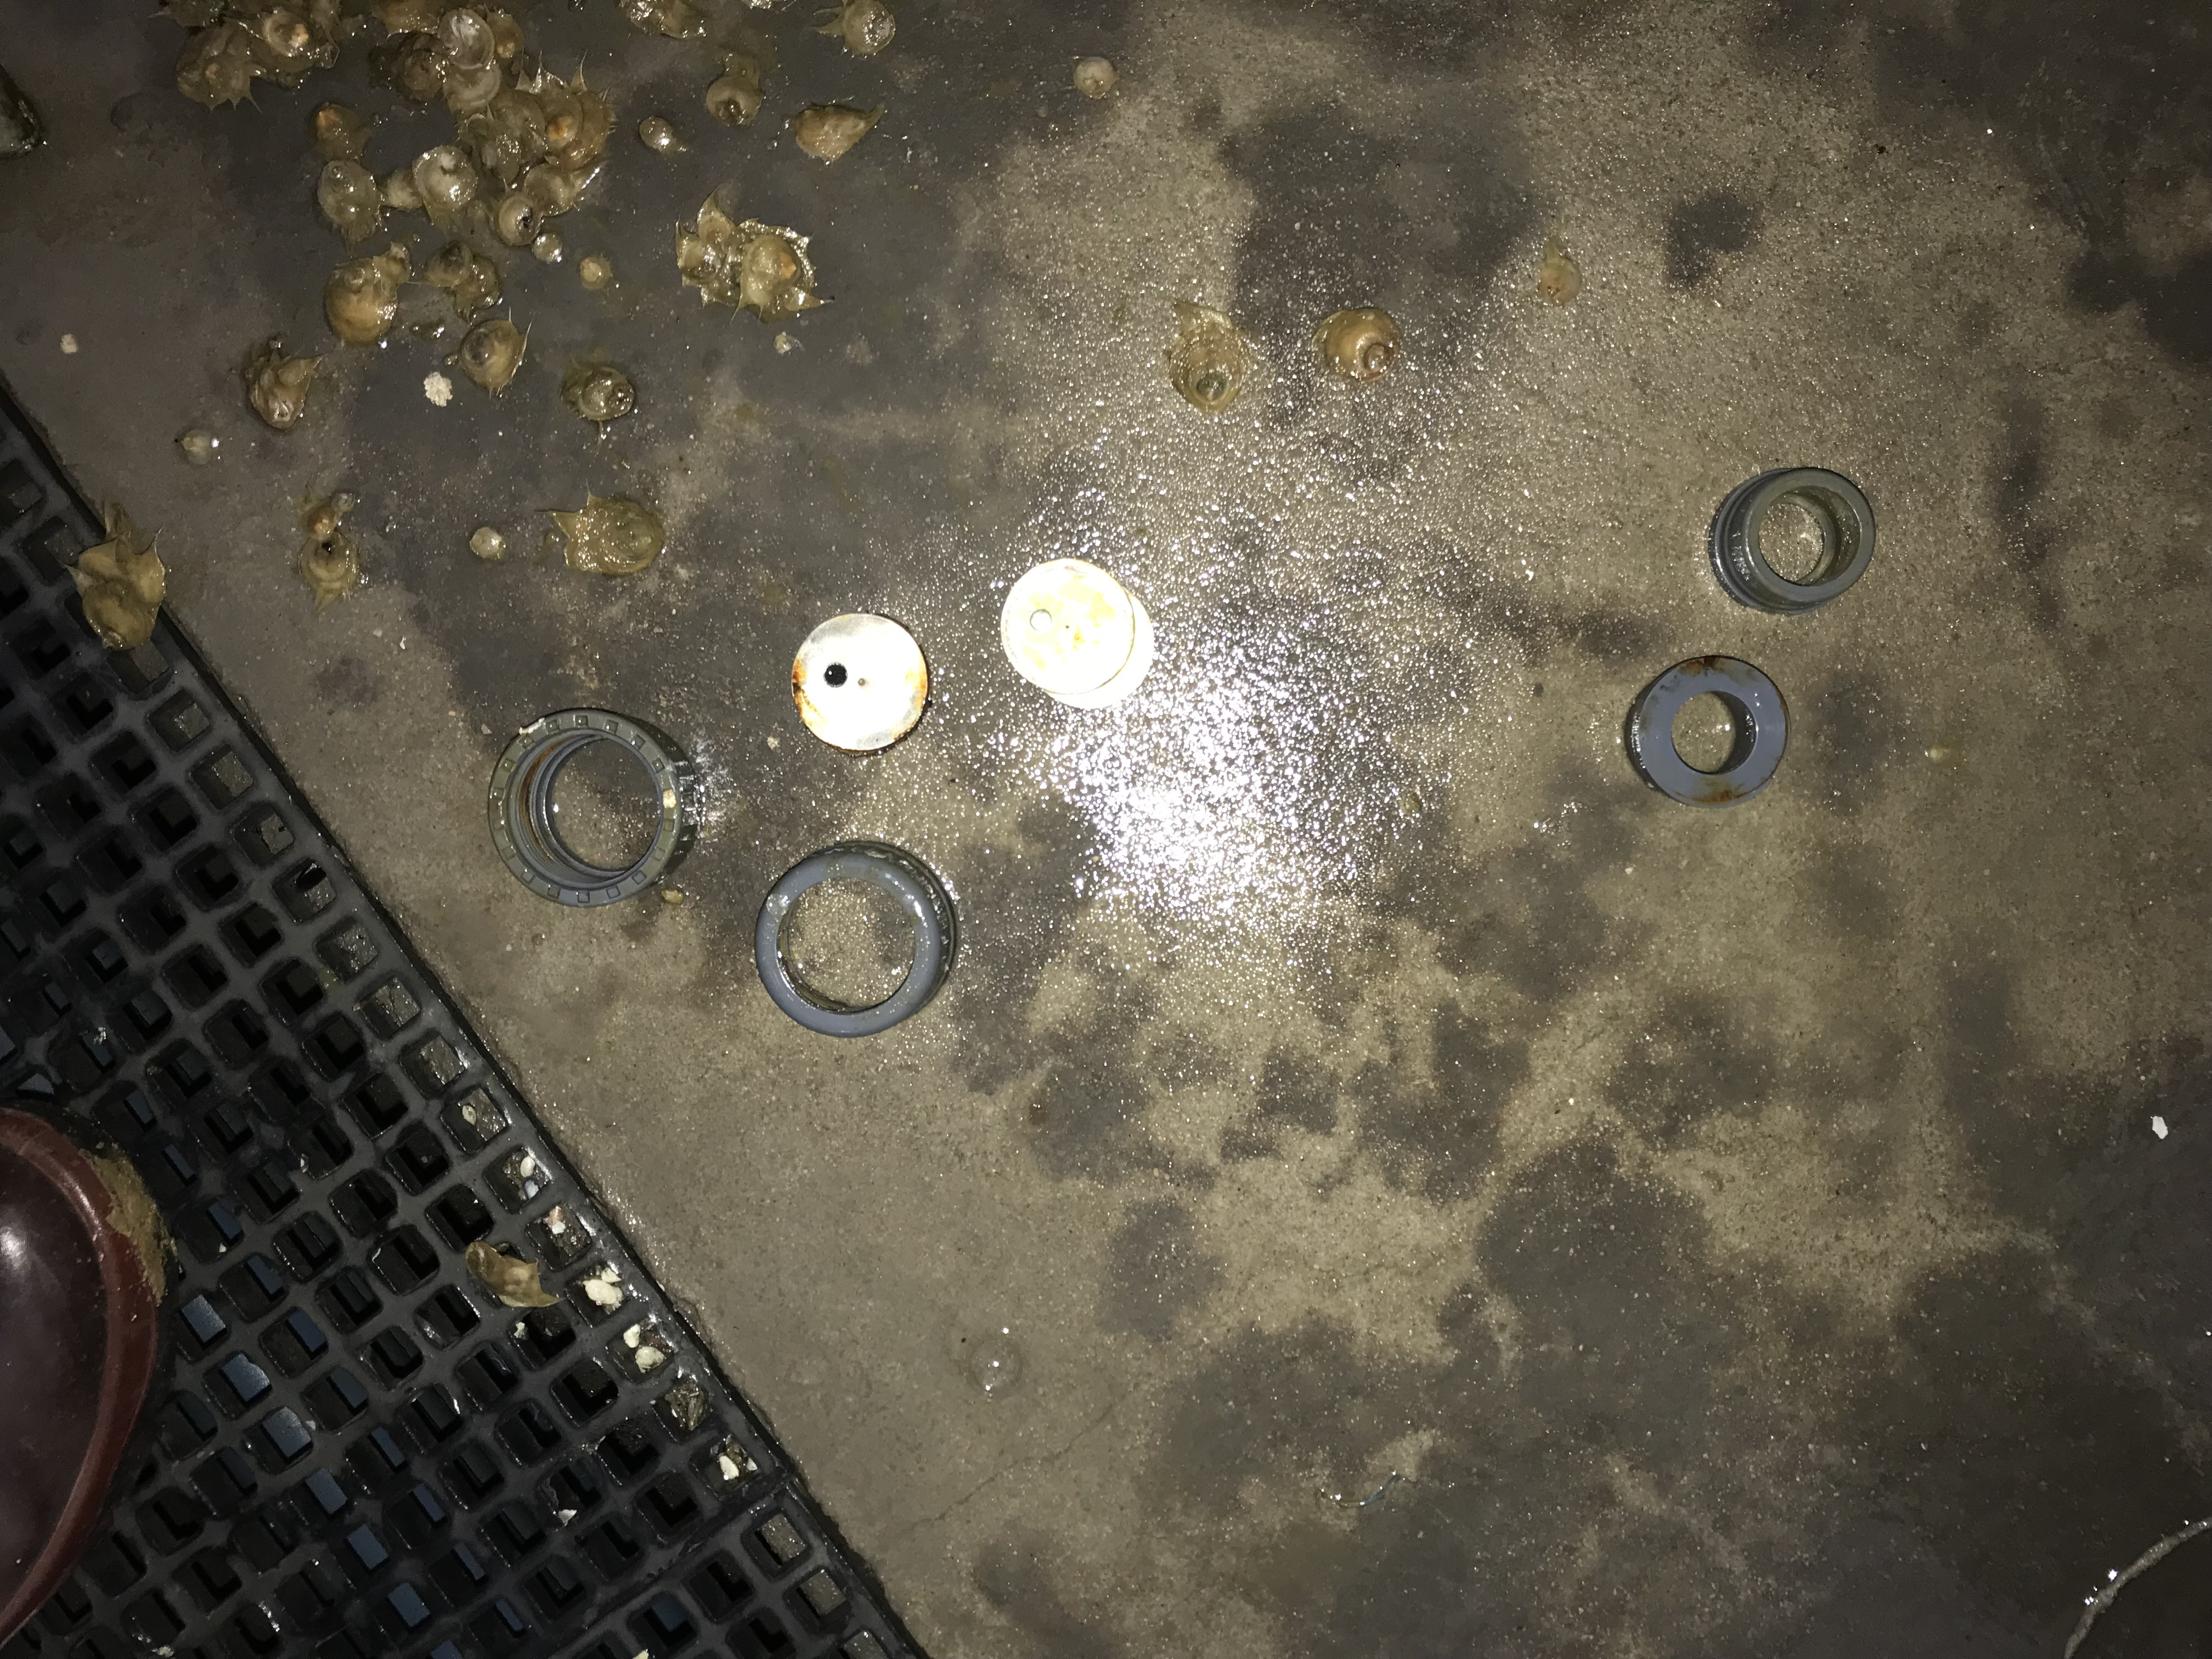
\includegraphics[width=0.5\textwidth,height=\textheight]{images/daf/nozzle_head.jpg}

}

\caption{\label{fig-dafnozzle}The disassembled DAF, saturated water,
discharge nozzle head.}

\end{figure}

\begin{enumerate}
\def\labelenumi{\arabic{enumi}.}
\setcounter{enumi}{21}
\tightlist
\item
  Inspect Nozzle parts for damage.

  \begin{itemize}
  \tightlist
  \item
    \emph{Take note of damage, if any, and proceed to next step}.
  \end{itemize}
\item
  Re-assemble respective parts from step 21.

  \begin{itemize}
  \tightlist
  \item
    \emph{Place the plate with the larger hole on top of the other,
    facing the opposite direction before inserting it into the Nozzle
    head}.
  \end{itemize}
\end{enumerate}

{If there are obvious signs of damage to the nozzles, they will have to
be replaced with new ones as soon as possible}. {Likely contact for new
Nozzles is Mr.~Jan Marais at Aqua services and engineering}.

\hypertarget{sec-clean-daf-tank}{%
\subsection{Clean tank}\label{sec-clean-daf-tank}}

\begin{enumerate}
\def\labelenumi{\arabic{enumi}.}
\setcounter{enumi}{23}
\tightlist
\item
  Turn on Jetty pump (Figure~\ref{fig-mcs}).
\item
  Close DAF drain valve No.~43 (Figure~\ref{fig-dafcomp}).
\item
  Fill a 1/4 of the DAF tank with sea water.
\item
  Turn off the Jetty pump.
\item
  Connect long hose pipe (16mm diameter) to a water tap.
\item
  Fasten long stick (approx. 2.2m length and 40mm diameter) to the
  opposite end of the hose pipe with cable ties.
\item
  Lower pipe into the DAF tank and open tap.
\item
  Use the water flow from the pipe to help agitate and thoroughly mix
  the sludge with the standing water.
\item
  Open the DAF drain valve and let the water-sludge mix drain out.

  \begin{itemize}
  \tightlist
  \item
    \emph{Continue mixing the sludge during draining}.
  \end{itemize}
\end{enumerate}

\begin{itemize}
\tightlist
\item
  \textbf{Fill a 1/4 of the DAF tank up and repeat if sludge not
  adequately cleared}.
\end{itemize}

\begin{enumerate}
\def\labelenumi{\arabic{enumi}.}
\setcounter{enumi}{32}
\tightlist
\item
  Climb out and remove the ladder.
\item
  Connect Nozzle manifold to the Saturated water inlet pipe.
\end{enumerate}

\hypertarget{resume-normal-operation}{%
\subsection{Resume normal operation}\label{resume-normal-operation}}

{Only resume normal system operation if there is no excess sludge
build-up at the bottom of the DAF tank}

\begin{enumerate}
\def\labelenumi{\arabic{enumi}.}
\setcounter{enumi}{34}
\tightlist
\item
  Switch on Jetty pump (Figure~\ref{fig-mcs}).
\item
  Close DAF drain valve No.~43.
\item
  Wait for DAF tank to fill up.

  \begin{itemize}
  \tightlist
  \item
    \emph{Lasts more than 30 minutes}.
  \end{itemize}
\item
  Open Main dump valve No.~18 (Figure~\ref{fig-dump-valve}).
\item
  Open Saturator isolating valve No.~36 (Figure~\ref{fig-sat-inlet}).
\item
  Switch on Saturator pump (Figure~\ref{fig-sat-power}).
\item
  Open Saturator discharge valve No.~42 (Figure~\ref{fig-sat-outlet}).
\end{enumerate}

\hypertarget{repairs}{%
\section{Repairs}\label{repairs}}

Under normal circumstances the Dissolved oxygen flotation (DAF) tank
acts as an initial filter in the Aquarium system, removing oils, grease
and any other suspended solids from the raw sea water intake. This is
achieved in conjunction with flocculant from the flocculant column
(Figure~\ref{fig-biofilter}) and micro air bubbles, supplied via nozzles
from the saturator column (Figure~\ref{fig-sat}) that are discharged at
the base of a smaller, central DAF column within the main DAF tank.
Flocculant coagulates the suspended material, which is then surrounded
and lifted by the micro-bubbles, before being skimmed off the top and
discharged through the waste outlet.

When the DAF performs sub-optimally, unfiltered, raw sea water
containing substances such as oils and heavy metals may enter the
Aquarium system. This can severely impair the display animals' health,
possibly leading to increased mortality rates. Consequently, the DAF
systems' performance should not be compromised for prolonged periods.

\hypertarget{problem-diagnosis}{%
\subsection{Problem diagnosis}\label{problem-diagnosis}}

Excess bubbling/large bubble formation was identified at the top of the
DAF by Mr.~Botes after a routine inspection round. Further consultation
with Mr.~Jan Marais, from Aqua Services and Engineering, narrowed the
problem down to a likely issue with the nozzles.

\hypertarget{tool-preparation}{%
\subsection{Tool preparation}\label{tool-preparation}}

\textbf{The tools used in Section~\ref{sec-daf-tool} were also used
here.}

\hypertarget{nozzle-inspection}{%
\subsection{Nozzle inspection}\label{nozzle-inspection}}

To inspect the nozzles, the DAF unit had to be drained of all liquid.

\hypertarget{drain-daf-1}{%
\subsubsection{Drain DAF}\label{drain-daf-1}}

\begin{itemize}
\tightlist
\item
  \textbf{Steps 1-6 will be completed inside the plant room}.
\end{itemize}

\begin{enumerate}
\def\labelenumi{\arabic{enumi}.}
\tightlist
\item
  Close Dump valve No.~18 (Figure~\ref{fig-dump-valve}).
\item
  Wait for the water level at the Prosonic HMU 860 to reach 90\%
  (Figure~\ref{fig-prosonic}).

  \begin{itemize}
  \tightlist
  \item
    \emph{Done to ensure enough sea water remains in circulation during
    the maintenance procedure}.
  \end{itemize}
\item
  Switch off the Jetty pump on the main control switchboard
  (Figure~\ref{fig-mcs}).

  \begin{itemize}
  \tightlist
  \item
    \emph{Prevents more water intake}.
  \end{itemize}
\item
  Switch off the Saturator pump.

  \begin{itemize}
  \tightlist
  \item
    \emph{Clipsal power outlet No.~2} (Figure~\ref{fig-sat-power}).
  \end{itemize}
\item
  Close the Saturator isolating valve No.~36
  (Figure~\ref{fig-sat-inlet}).

  \begin{itemize}
  \tightlist
  \item
    \emph{Feeds the Saturator system}.
  \end{itemize}
\item
  Close the Saturator discharge valve (No.~42) to the DAF tank
  (Figure~\ref{fig-sat-outlet}).
\end{enumerate}

\begin{itemize}
\tightlist
\item
  \textbf{Steps 3 - 6 prevent water flow into the DAF unit during the
  maintenance procedure}.
\end{itemize}

\begin{enumerate}
\def\labelenumi{\arabic{enumi}.}
\setcounter{enumi}{6}
\tightlist
\item
  Opened DAF drain valve No.~43 (Figure~\ref{fig-dafcomp}).
\item
  Allowed DAF to drain completely.
\end{enumerate}

\begin{itemize}
\tightlist
\item
  \textbf{Some water still remained in central DAF column after
  draining}
\end{itemize}

{Once completely drained, excess sludge could be seen accumulated at the
bottom of the DAF tank}

\hypertarget{extract-nozzle-manifold-and-associated-parts}{%
\subsubsection{Extract Nozzle manifold and associated
parts}\label{extract-nozzle-manifold-and-associated-parts}}

{This is a job for a minimum of 2 people}

\begin{enumerate}
\def\labelenumi{\arabic{enumi}.}
\setcounter{enumi}{8}
\tightlist
\item
  Uncoupled the Nozzle manifold from the Saturated water inlet pipe.

  \begin{itemize}
  \tightlist
  \item
    \emph{Used a monkey wrench}.
  \end{itemize}
\item
  Pulled Nozzle manifold out of central DAF column for further
  inspection.

  \begin{itemize}
  \tightlist
  \item
    \emph{One of three Nozzle heads was missing and there was some
    blockage around the Nozzle outlets due to biofouling}.
  \end{itemize}
\item
  Allowed pungent fumes emitted by the sludge build up to clear
  overnight.

  \begin{itemize}
  \tightlist
  \item
    \emph{Prolonged inhalation of concentrated methane gas can result in
    loss of consciousness}.
  \end{itemize}
\item
  Lowered ladder into DAF tank, against central column and climbed in.

  \begin{itemize}
  \tightlist
  \item
    \emph{Person climbing in should be small enough to fit through the
    top of the DAF tank}.
  \end{itemize}
\item
  Siphoned water out of the central DAF column and into the main DAF
  tank, where it was discharged via valve No.~43
  (Figure~\ref{fig-dafcomp}).

  \begin{itemize}
  \tightlist
  \item
    \emph{Used a 50mm diameter hose}.
  \item
    \emph{Lowered hose into water, created a vacuum inside the hose and
    kept outlet at lower level than inlet to generate flow out of
    central column}.
  \end{itemize}
\item
  Retrieved missing Nozzle parts from central DAF column
  (Figure~\ref{fig-dafnozzle}).

  \begin{itemize}
  \tightlist
  \item
    \emph{Used Fish scoop net and bucket}.
  \item
    \emph{Had to scoop out some sludge first to get to the lost parts}.
  \end{itemize}
\item
  Used the fish scoop net to discard (into bucket) any remaining sludge
  after retrieving the lost Nozzle parts.
\item
  Removed ladder.
\item
  Dismantled and cleaned the Nozzle manifold, Nozzle heads and any
  accompanying parts.

  \begin{itemize}
  \tightlist
  \item
    \emph{Found two, small circular plates within the Nozzles}
    (Figure~\ref{fig-dafnozzle}).
  \item
    \emph{Both had a single hole along their periphery. One smaller than
    the other}.
  \end{itemize}
\item
  Inspected the Nozzle parts for damage.

  \begin{itemize}
  \tightlist
  \item
    \emph{Parts were not damaged}.
  \end{itemize}
\item
  Re-assembled respective parts from step 17.

  \begin{itemize}
  \tightlist
  \item
    \emph{Placed the plate with the larger hole on top of the other,
    facing the opposite direction before inserting it into the Nozzle
    head}.
  \end{itemize}
\item
  Connected the Nozzle manifold to the Saturated water inlet pipe.
\end{enumerate}

{In case of damage to Nozzle parts, contact Mr.~Jan Marais, at Aqua
services and engineering, for new Nozzles}.

\hypertarget{resume-normal-operation-1}{%
\subsubsection{Resume normal
operation}\label{resume-normal-operation-1}}

\textbf{Once all sludge has been removed (see
Section~\ref{sec-daf-maintain} for clean up procedure) normal system
operation can be started}.

\begin{enumerate}
\def\labelenumi{\arabic{enumi}.}
\setcounter{enumi}{20}
\tightlist
\item
  Switch on Jetty pump (Figure~\ref{fig-mcs}).
\item
  Close DAF drain valve No.~43 (Figure~\ref{fig-dafcomp}).
\item
  Wait for DAF tank to fill up.

  \begin{itemize}
  \tightlist
  \item
    \emph{Lasts more than 30 minutes}.
  \end{itemize}
\item
  Open main dump valve No.~18 (Figure~\ref{fig-dump-valve}).
\item
  Open Saturator isolating valve No.~36 (Figure~\ref{fig-sat-inlet}).
\item
  Switch on Saturator pump (Figure~\ref{fig-sat-power}).
\item
  Open Saturator discharge valve No.~42 (Figure~\ref{fig-sat-outlet}).
\end{enumerate}

\newpage

\hypertarget{sec-fractionator}{%
\chapter{Foam Fractionator}\label{sec-fractionator}}

The Foam fractionator is found next to the DAF tank
(Figure~\ref{fig-biofilter}). It has an outlet and drain valve connected
to the outside of it's main tank (Figure~\ref{fig-foamcomp}).

\begin{figure}[H]

\begin{minipage}[t]{0.33\linewidth}

{\centering 

\raisebox{-\height}{

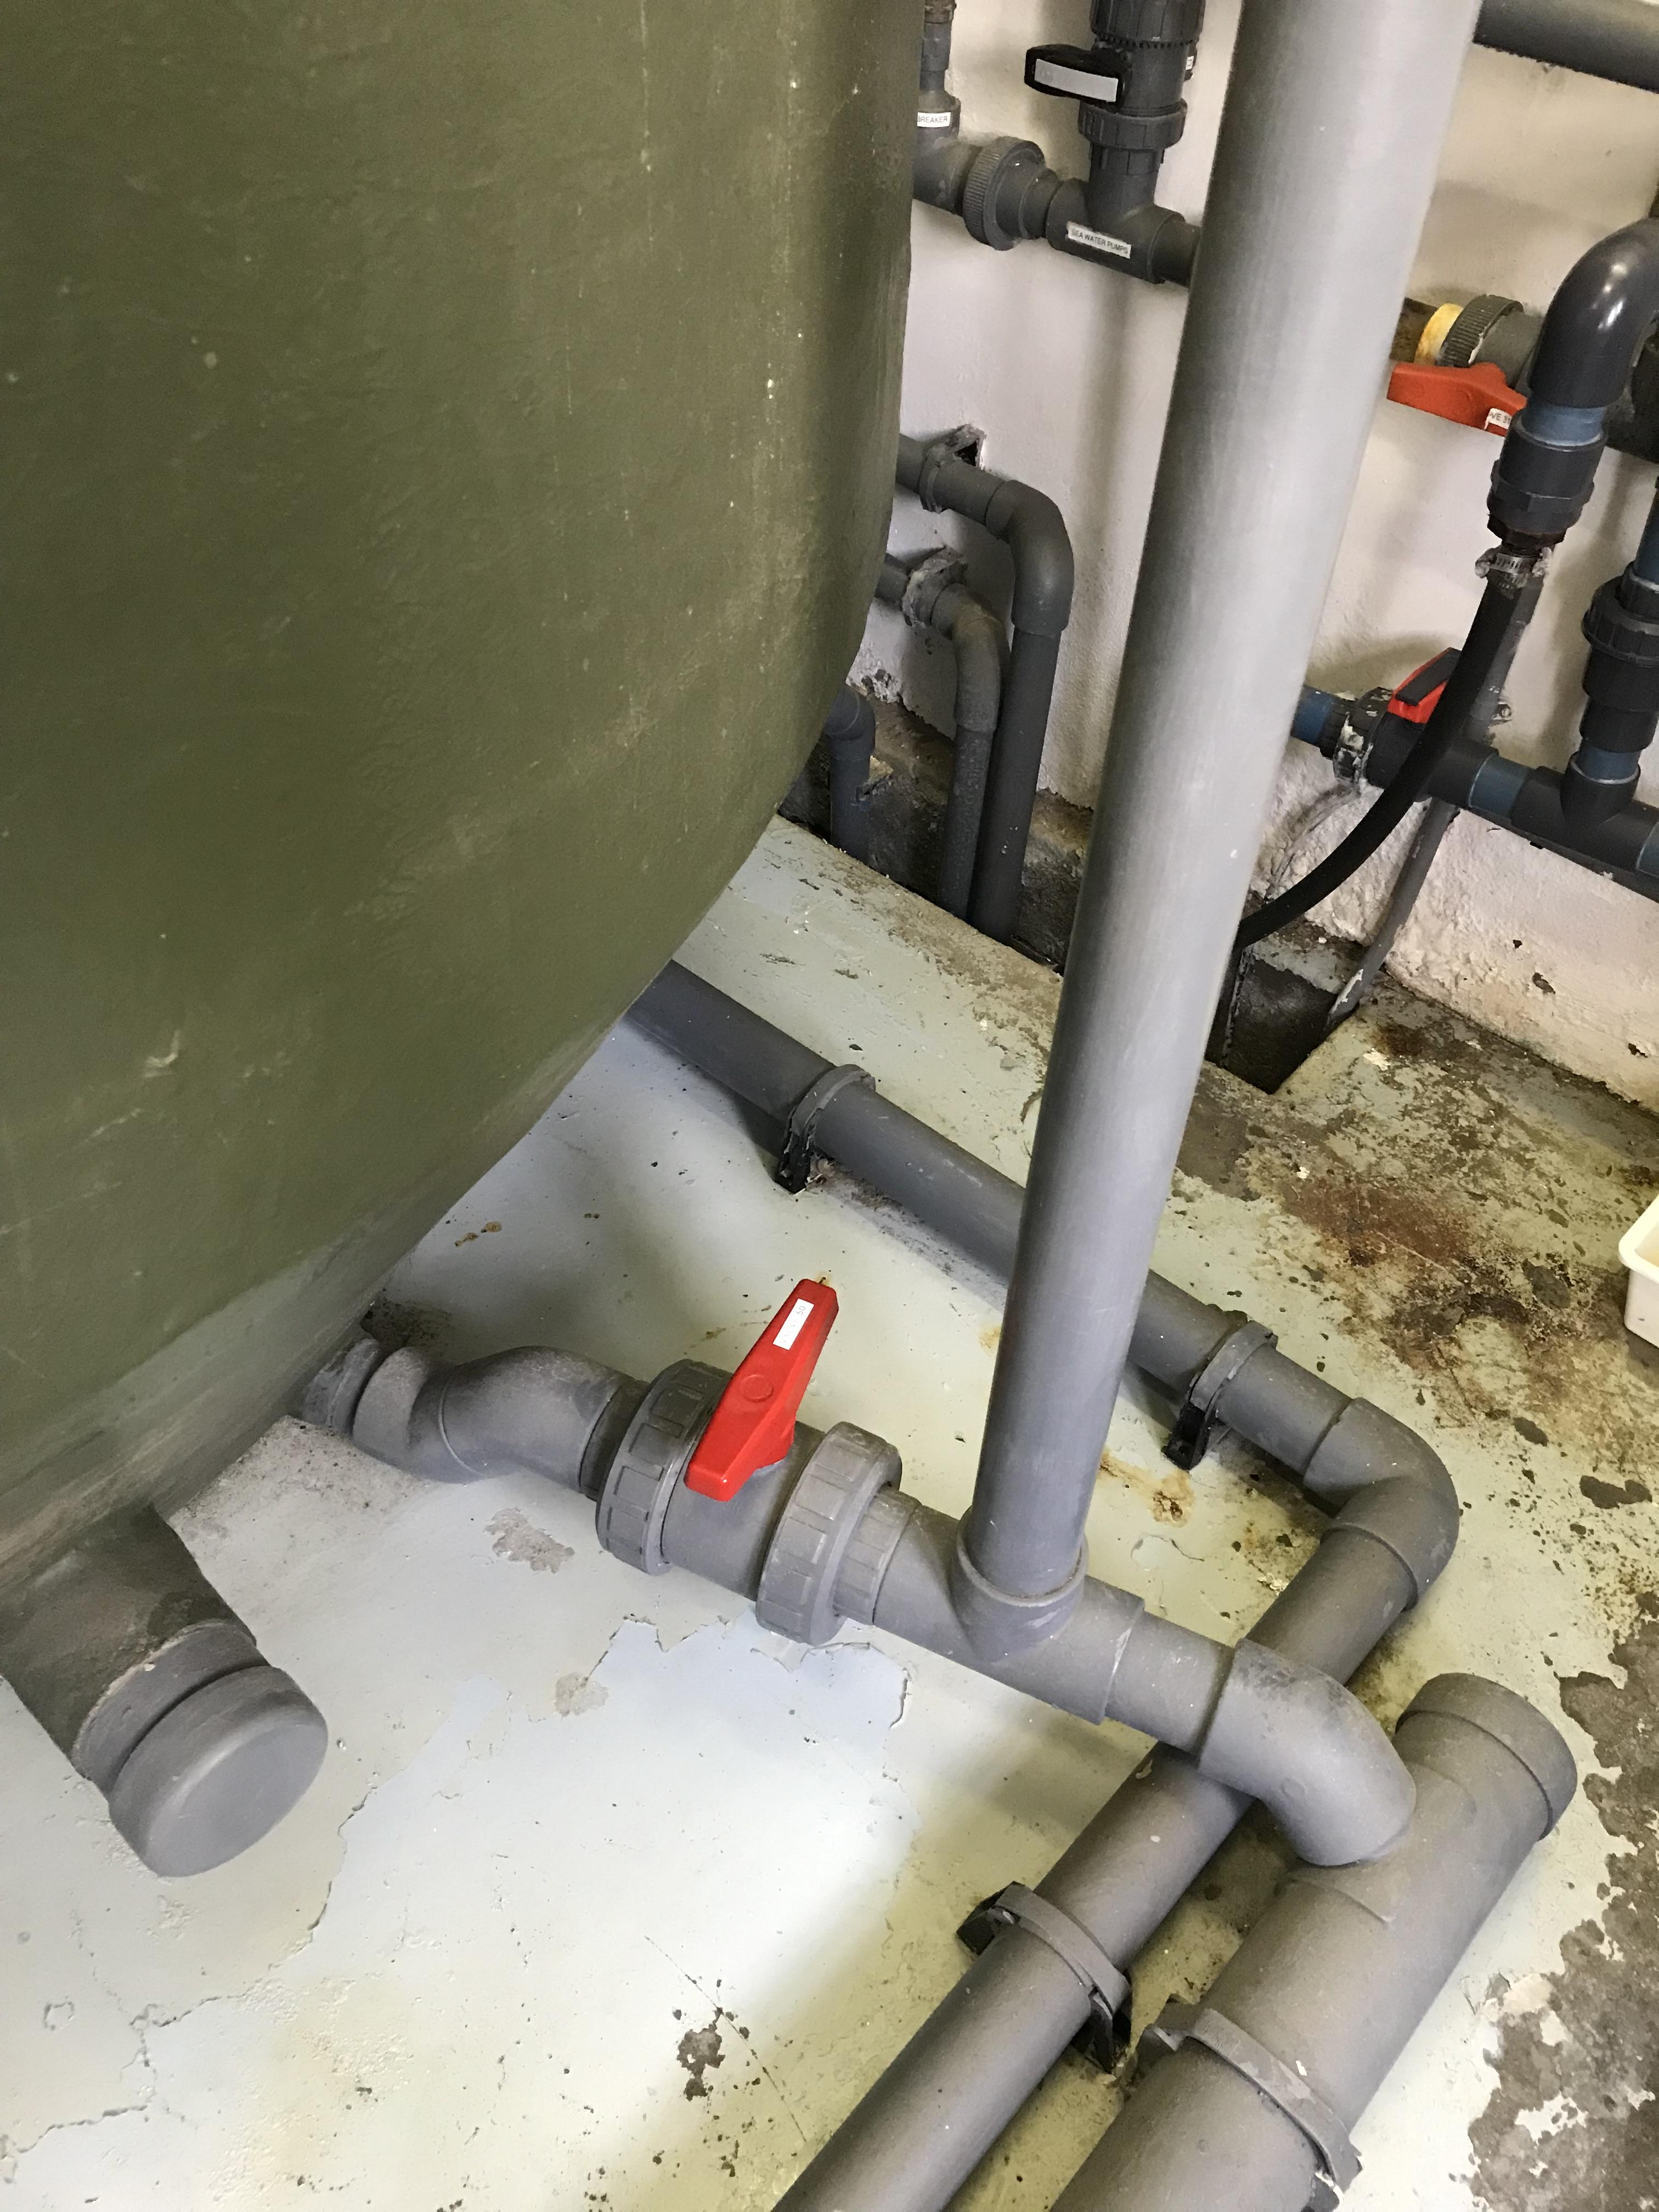
\includegraphics{images/foam_frac/drain2.jpg}

}

}

\subcaption{\label{fig-frac-drain}Drain valve}
\end{minipage}%
%
\begin{minipage}[t]{0.33\linewidth}

{\centering 

\raisebox{-\height}{

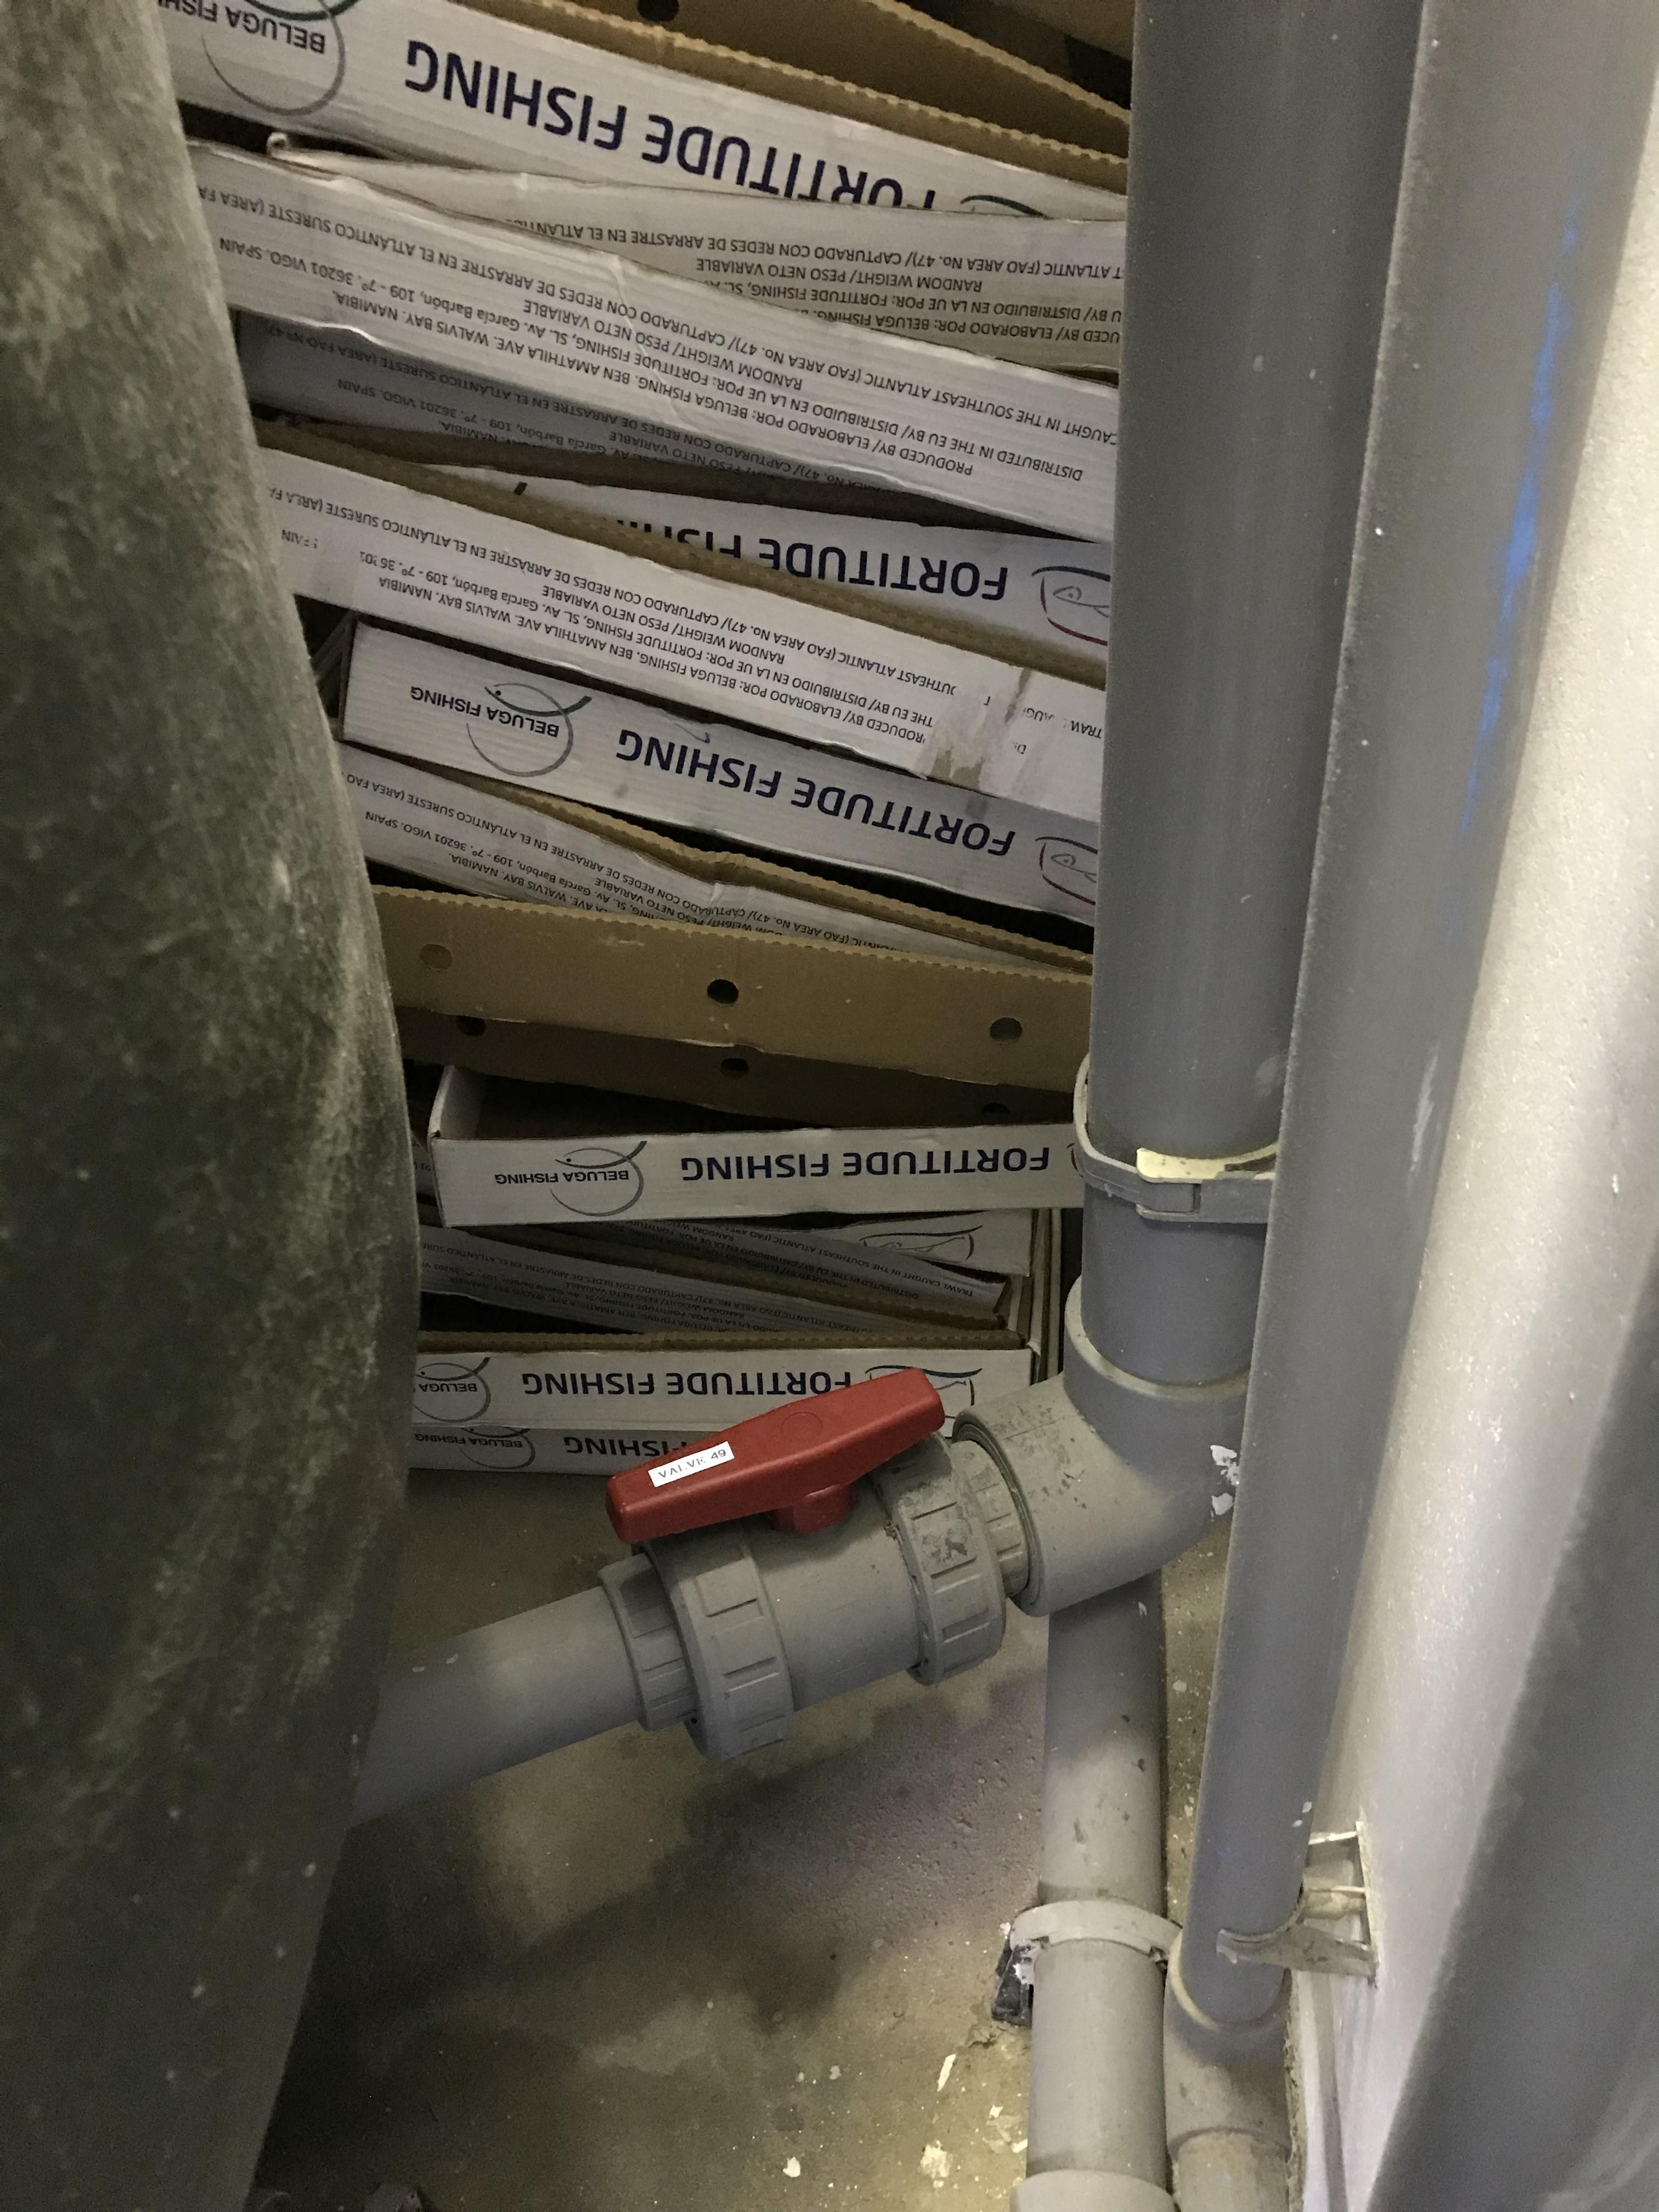
\includegraphics{images/foam_frac/outlet2.jpg}

}

}

\subcaption{\label{fig-frac-outlet}Outlet valve}
\end{minipage}%
%
\begin{minipage}[t]{0.33\linewidth}

{\centering 

\raisebox{-\height}{

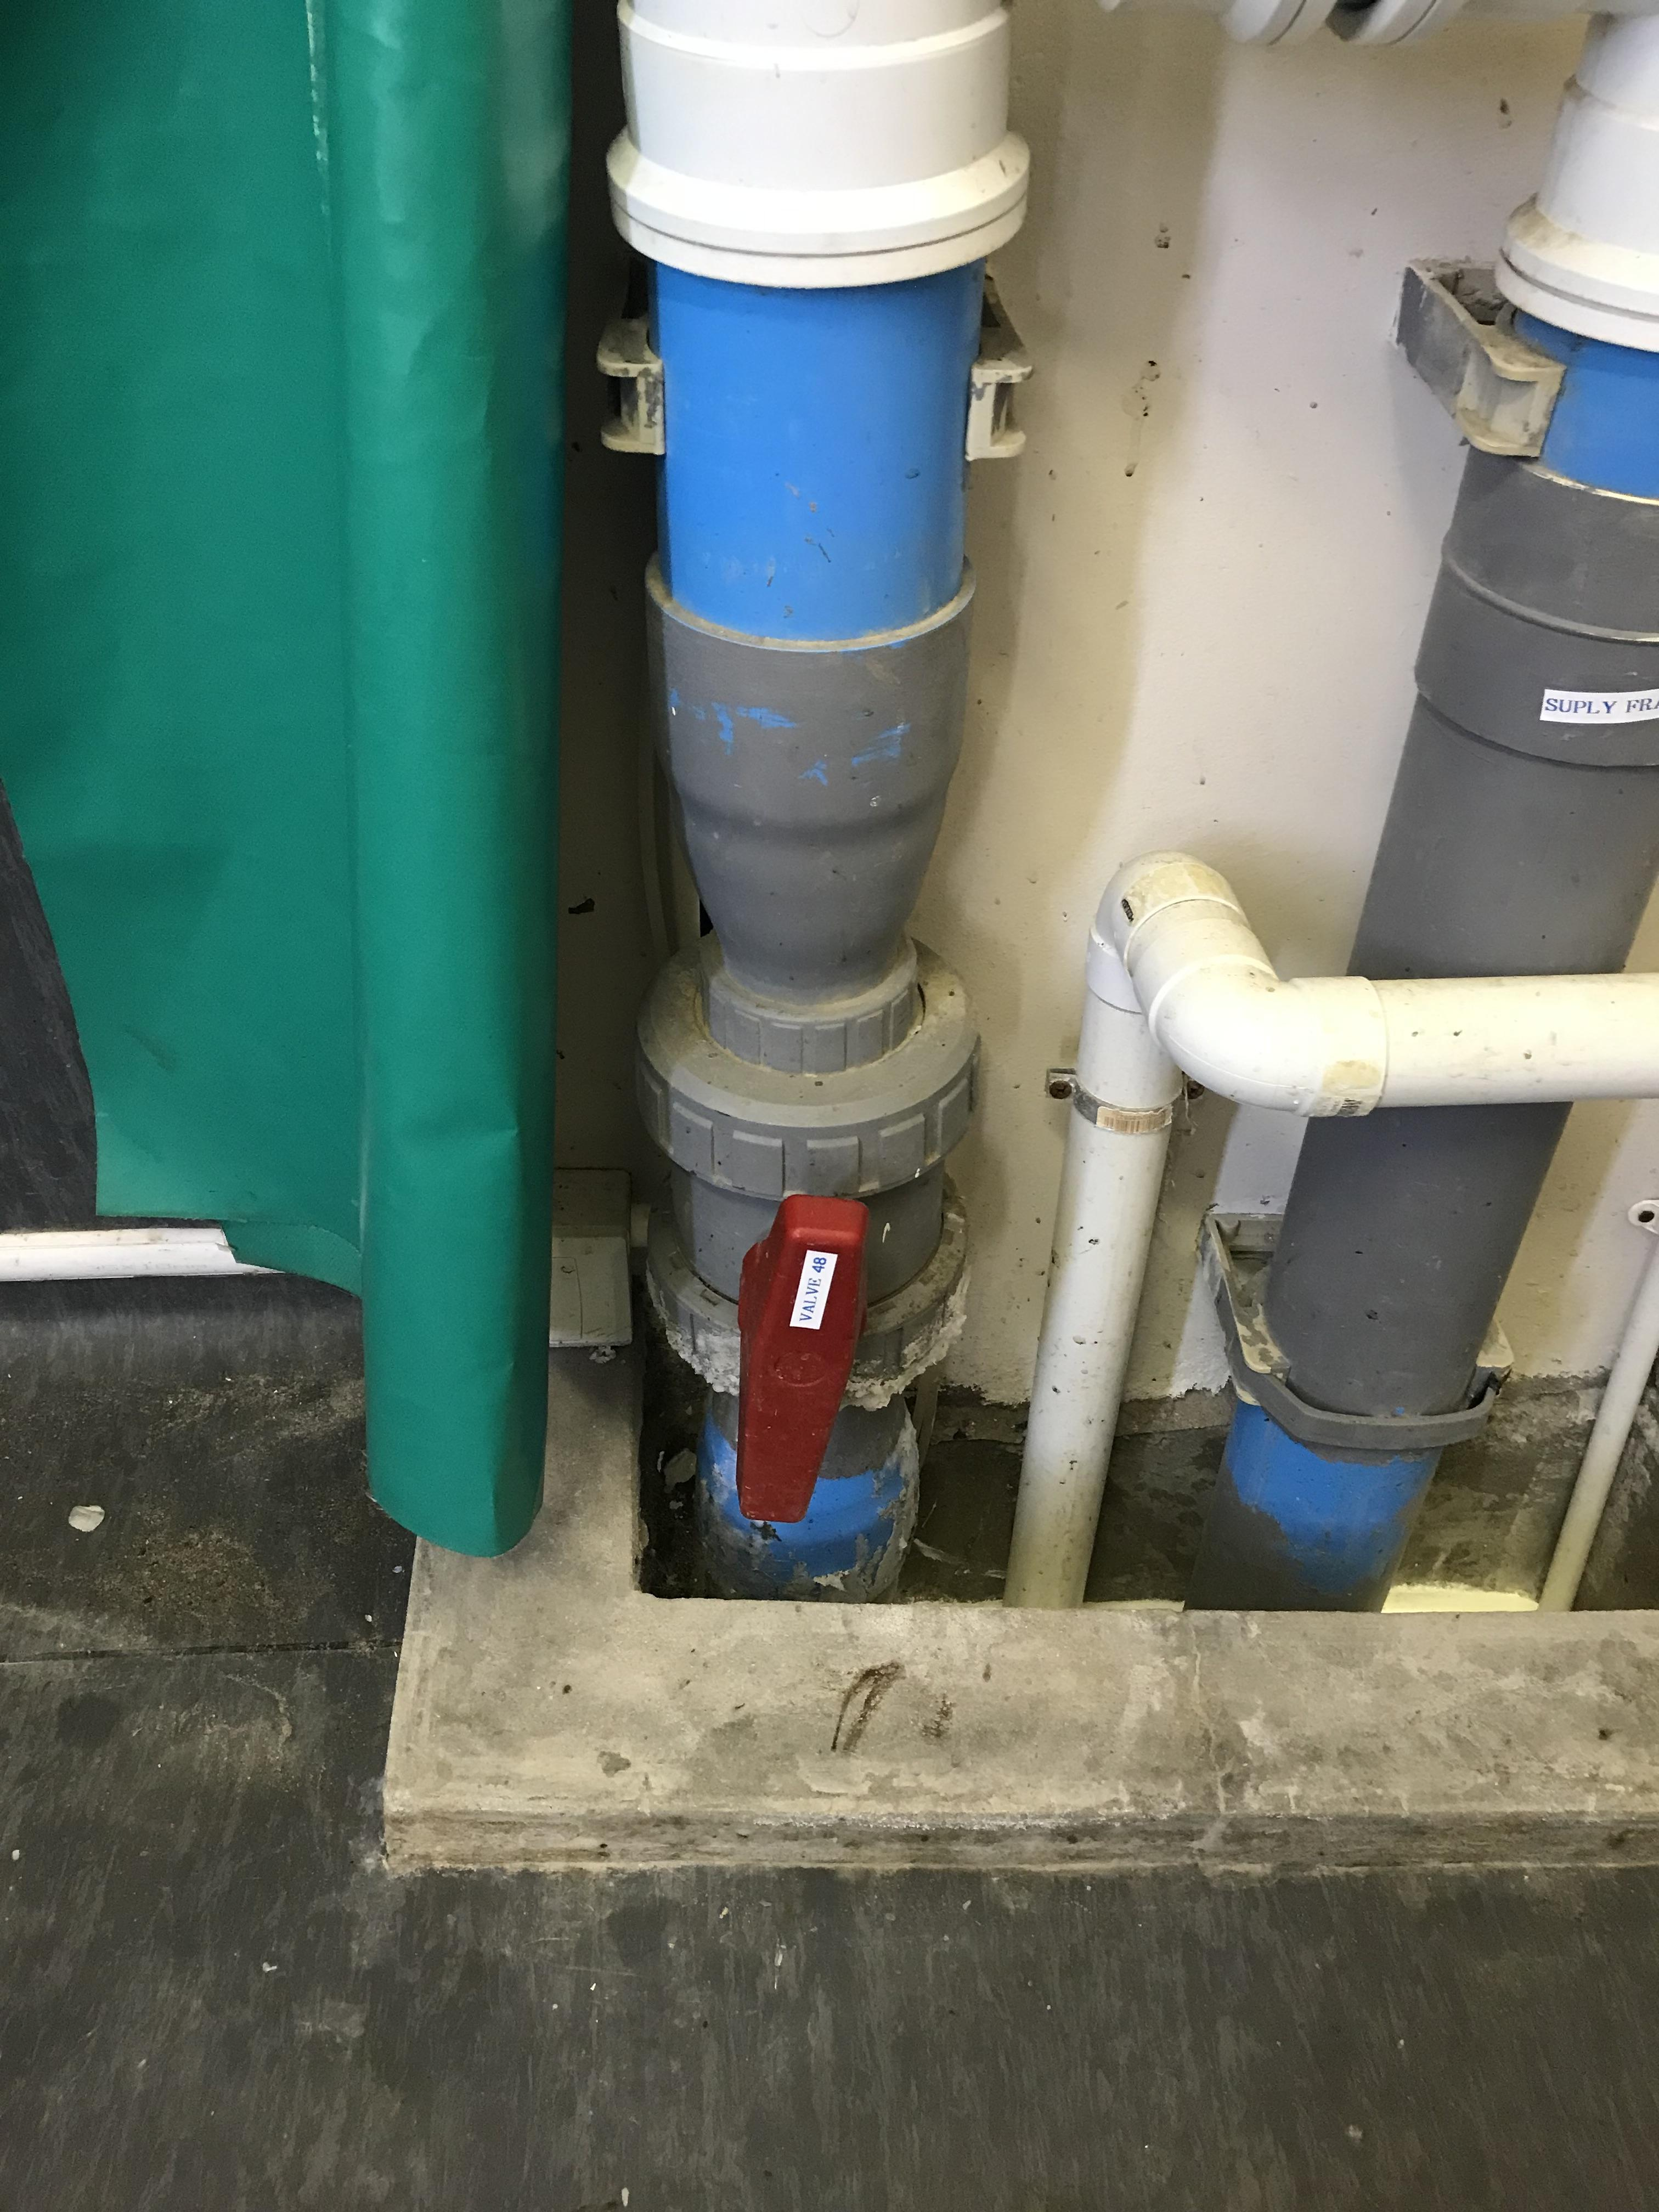
\includegraphics{images/foam_frac/supply2.jpg}

}

}

\subcaption{\label{fig-frac-inlet}Inlet valve}
\end{minipage}%

\caption{\label{fig-foamcomp}The main components used to control water
flow into and out of the foam fractionator.}

\end{figure}

The inner tank consists of an air inlet pipe, water inlet pipe and four
collection strainers that convey water to the fractionator's discharge
pipe (Figure~\ref{fig-foaminner}).

\begin{figure}[H]

{\centering 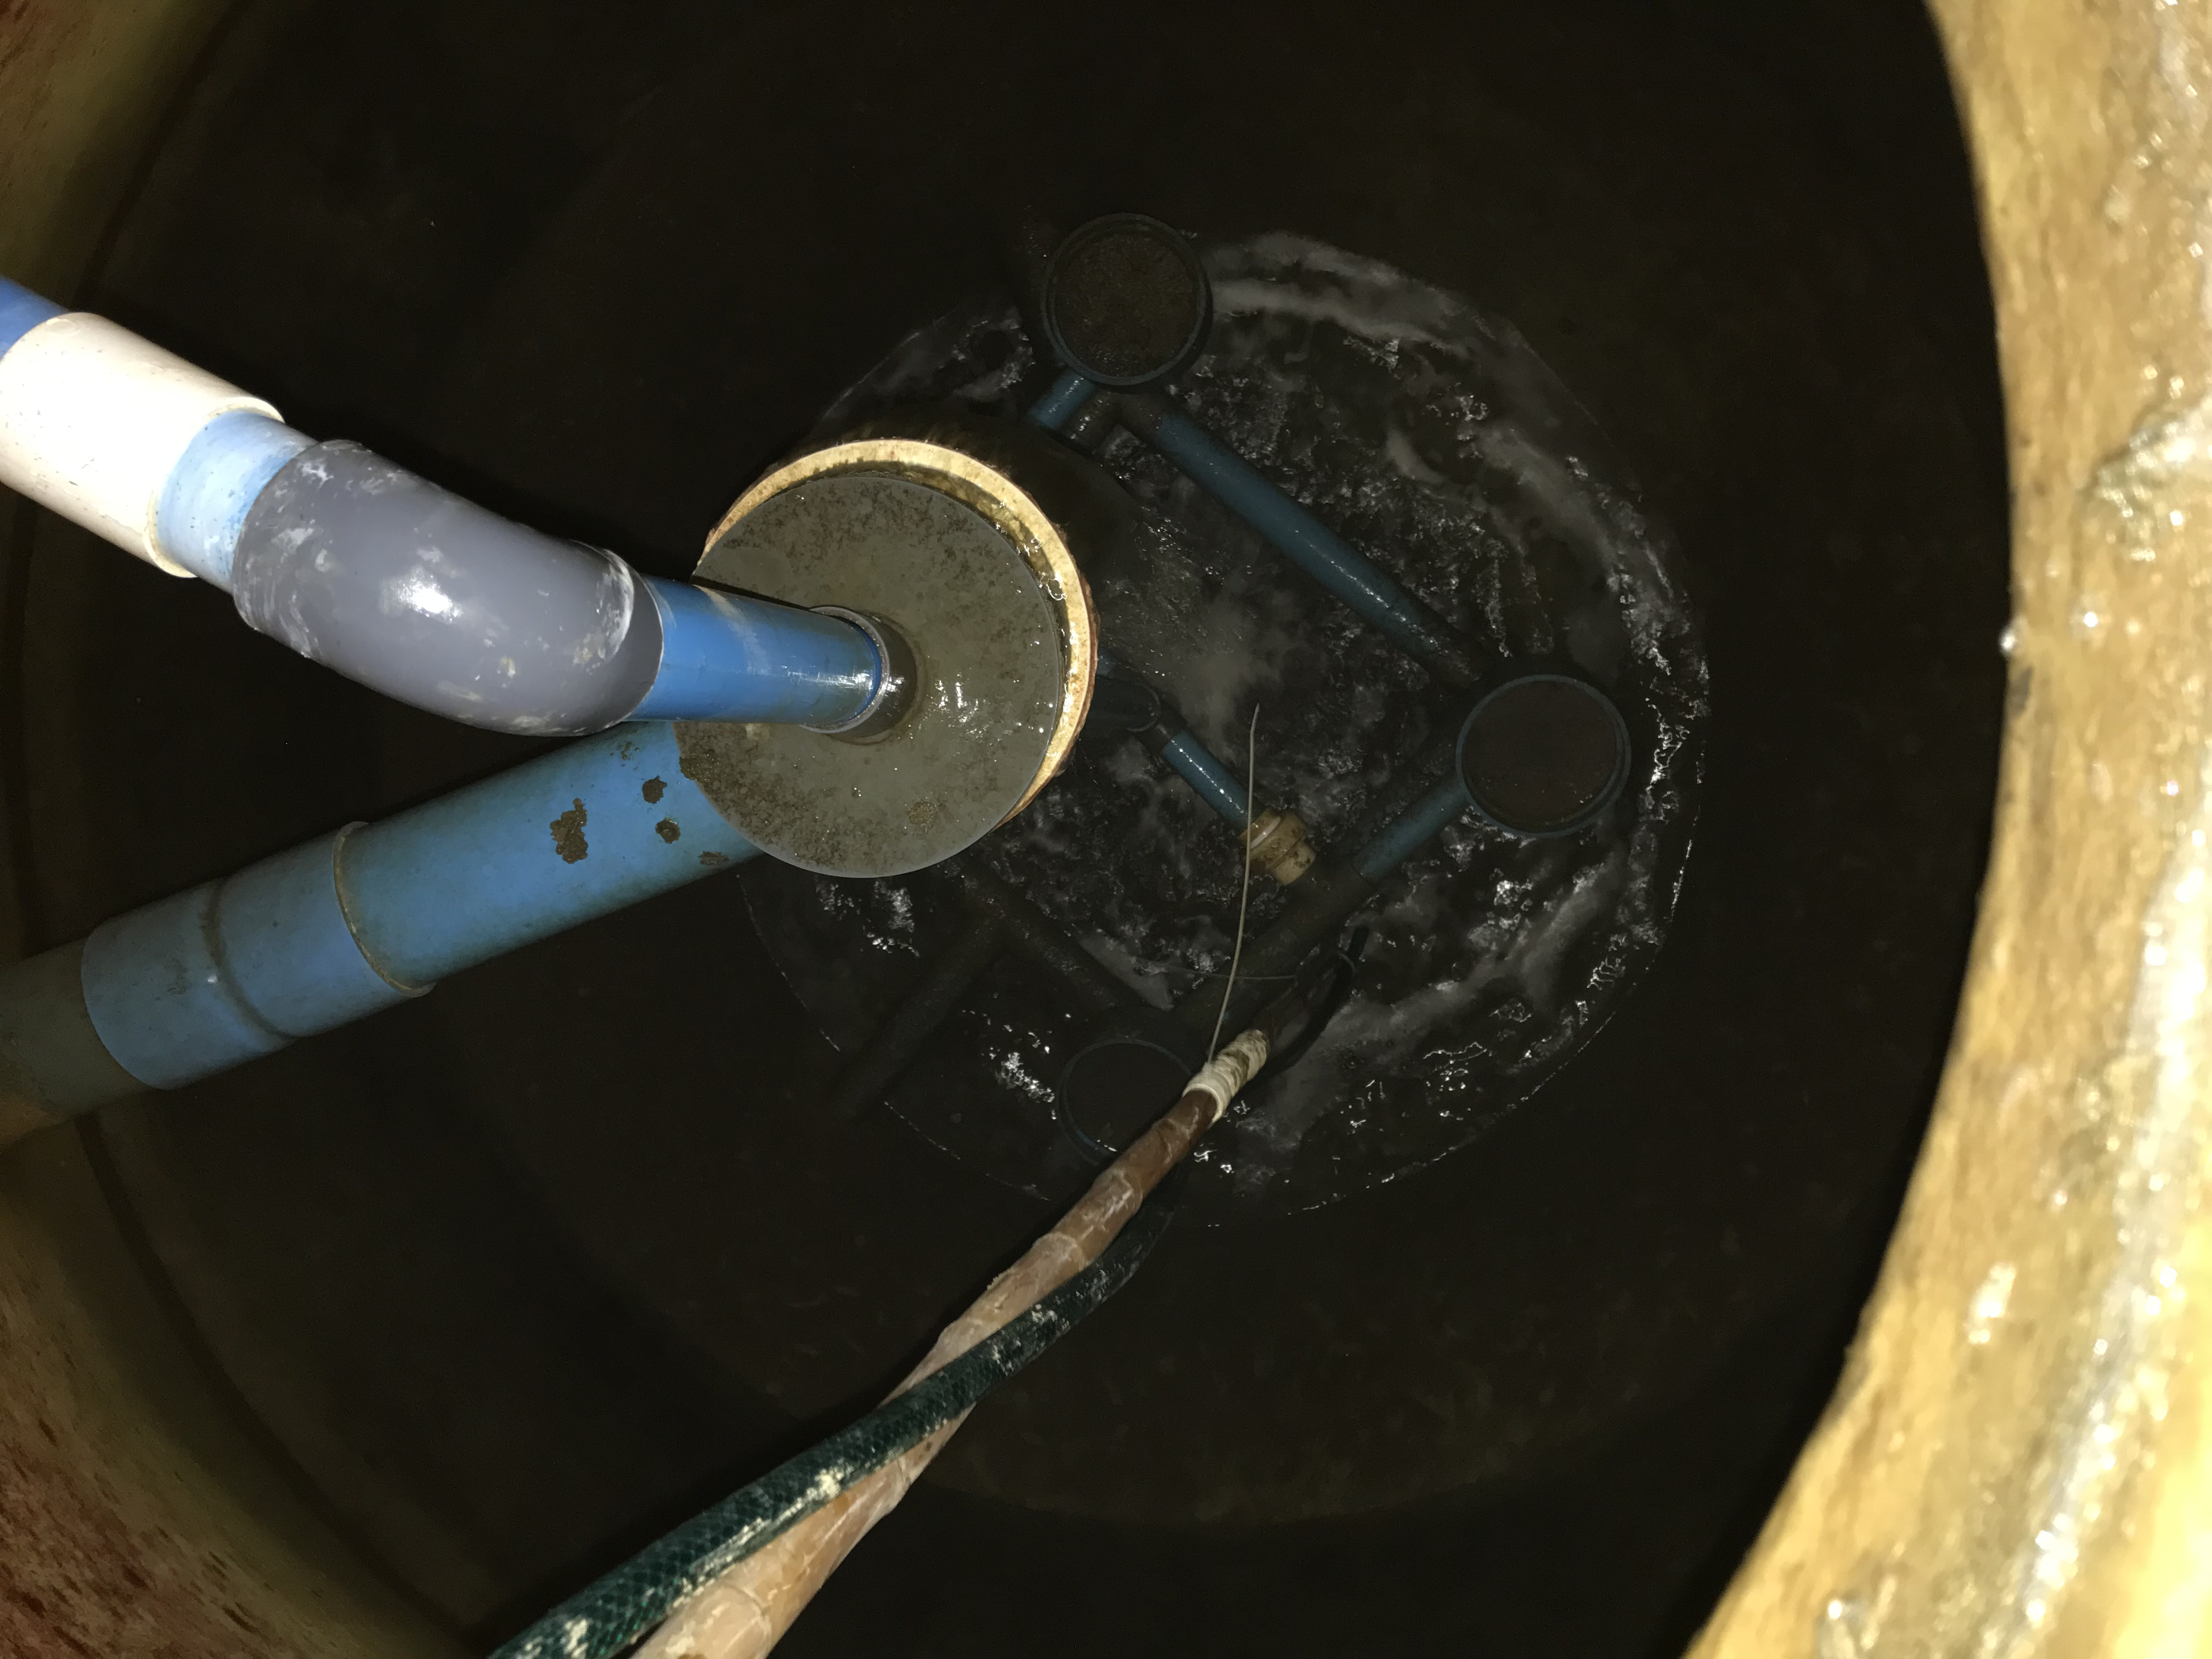
\includegraphics[width=0.5\textwidth,height=\textheight]{images/foam_frac/foam_inner.jpg}

}

\caption{\label{fig-foaminner}Image displaying the air inlet (top),
water inlet (center) and collection strainers (bottom) found inside the
foam fractionator.}

\end{figure}

\hypertarget{sec-frac-main}{%
\section{Maintenance}\label{sec-frac-main}}

{The maintenance procedure described for the Foam fractionator (referred
to as ``the Fractionator'' throughout) should be completed once every
year}.

\hypertarget{tool-preparation-1}{%
\subsection{Tool preparation}\label{tool-preparation-1}}

Use the same tools used for the DAF maintenance procedure
(Section~\ref{sec-daf-tool}).

\textbf{To conduct annual maintenance, the Fractionator has to be
drained completely}.

\hypertarget{sec-drain-frac}{%
\subsection{Drain the Fractionator}\label{sec-drain-frac}}

\begin{enumerate}
\def\labelenumi{\arabic{enumi}.}
\tightlist
\item
  Close Dump valve (No.~18), found in the Plant room.
\item
  Wait for the water level at the Prosonic HMU 860 to reach 90\%.

  \begin{enumerate}
  \def\labelenumii{\roman{enumii})}
  \tightlist
  \item
    \emph{Done to ensure enough sea water remains in circulation during
    the maintenance procedure}.
  \end{enumerate}
\item
  Turn off the Jetty pump on the Main control switchboard.

  \begin{enumerate}
  \def\labelenumii{\roman{enumii})}
  \tightlist
  \item
    \emph{Prevents the intake of more water}.
  \end{enumerate}
\item
  Turn off the Fractionator blowers on the Main control switchboard
  (Figure~\ref{fig-mcs}).
\item
  Close the Fractionator outlet valve No.~49
  (Figure~\ref{fig-frac-outlet}).

  \begin{enumerate}
  \def\labelenumii{\roman{enumii})}
  \tightlist
  \item
    \emph{Prevents the discharge of more water into the Compensation
    sump}
  \end{enumerate}
\item
  Close the Fractionator inlet valve No.~48
  (Figure~\ref{fig-frac-inlet}).

  \begin{enumerate}
  \def\labelenumii{\roman{enumii})}
  \tightlist
  \item
    \emph{Prevents the flow of more water into the Fractionator}.
  \end{enumerate}
\item
  Open the Fractionator drain valve No.~50
  (Figure~\ref{fig-frac-drain}).
\item
  Let the Fractionator drain completely.
\end{enumerate}

\hypertarget{inspect-internal-plumbing}{%
\subsection{Inspect internal plumbing}\label{inspect-internal-plumbing}}

\begin{enumerate}
\def\labelenumi{\arabic{enumi}.}
\setcounter{enumi}{8}
\tightlist
\item
  Ensure that all pipes, fittings, strainers and any other fixtures
  required to convey water are appropriately arranged and attached
  within the tank (Figure~\ref{fig-foaminner}).

  \begin{enumerate}
  \def\labelenumii{\roman{enumii})}
  \tightlist
  \item
    \textbf{See Section~\ref{sec-foam-realign} for example of steps
    taken to realign strainers found at the bottom of the Fractionator}.
  \end{enumerate}
\end{enumerate}

\hypertarget{sec-foam-clean}{%
\subsection{Clean tank}\label{sec-foam-clean}}

{This will only need to be done if there is a build-up of excess sludge
at the bottom of the tank, which is not likely to happen because mostly
filtered water enters the Fractionator from the Main tank floor}. {All
cleaning can be done from the top of the Fractionator}.

\begin{itemize}
\tightlist
\item
  \textbf{Skip cleaning procedure (steps 10-21) if the bottom of the
  Fractionator is already clean}.
\end{itemize}

\begin{enumerate}
\def\labelenumi{\arabic{enumi}.}
\setcounter{enumi}{9}
\tightlist
\item
  Connect a long hose pipe (16mm diameter) to a water tap.
\item
  Spray off any excess sludge in the Waste collection trough around the
  Fractionator periphery, found approximately 1/3 of the way from the
  top of the tank.
\item
  Turn off the tap.
\item
  Close the Fractionator drain valve No.~50
  (Figure~\ref{fig-frac-drain}).
\item
  Open the Fractionator inlet valve No.~48
  (Figure~\ref{fig-frac-inlet}).
\item
  Fill a 1/4 of the Fractionator with sea water.
\item
  Close the Fractionator inlet valve (No.~48).
\item
  Fasten a long stick (approx. 2.2m length and 40mm diameter) to the
  outlet end of the hose pipe with cable ties.
\item
  Lower the pipe into the Fractionator and open the tap.
\item
  Use the water flow from the pipe to help agitate and thoroughly mix
  the sludge trapped at the bottom of the tank, as well as on the
  strainers, with the standing water.
\item
  Open the Fractionator drain valve and let the water-sludge mix drain
  out.

  \begin{enumerate}
  \def\labelenumii{\roman{enumii})}
  \tightlist
  \item
    \emph{Continue mixing the sludge during draining}.
  \end{enumerate}
\end{enumerate}

\begin{itemize}
\tightlist
\item
  \textbf{Fill a 1/4 of the Fractionator tank up and repeat if sludge
  not adequately cleared}.
\end{itemize}

\begin{enumerate}
\def\labelenumi{\arabic{enumi}.}
\setcounter{enumi}{20}
\tightlist
\item
  Close the tap and remove the pipe from the tank.
\end{enumerate}

\hypertarget{sec-foam-resume}{%
\subsection{Resume normal operation}\label{sec-foam-resume}}

{Only resume normal system operation if there is no excess sludge
build-up at the bottom of the Fractionator}.

\begin{enumerate}
\def\labelenumi{\arabic{enumi}.}
\setcounter{enumi}{21}
\tightlist
\item
  Close the Fractionator drain valve (No.~50).
\item
  Open the Fractionator inlet valve (No.~48).
\item
  Turn on the Jetty pump .
\item
  Wait for the Fractionator to fill up.

  \begin{enumerate}
  \def\labelenumii{\roman{enumii})}
  \tightlist
  \item
    \emph{Lasts more than 30 minutes}.
  \end{enumerate}
\item
  Open the Fractionator outlet valve (No.~49).\\
\item
  Open the Dump valve No.~18 (Figure~\ref{fig-dump-valve}).
\item
  Turn on the Fractionator blowers (Figure~\ref{fig-mcs}).
\end{enumerate}

\hypertarget{repairs-1}{%
\section{Repairs}\label{repairs-1}}

During normal operation the Foam fractionator helps remove excess
protein from the recirculated Aquarium water. Air bubbles released from
a series of diffusers near the base of the tank, aggregate the suspended
protein by exploiting the amphipathicity of protein. This creates a foam
that, because of its' lower density, rises to the Fractionator water
surface where it is skimmed off the top. Waste generated through this
process is then conveyed to the Fractionator drain valve
(Figure~\ref{fig-foamcomp}), and discharged along with sludge that may
have accumulated at the bottom. The skimmed water settles back into the
fractionator. It is then discharged near the Fractionators' base after
passing through four strainers, fastened near the ends of two parallel
pipes, which are joined to each other by a central pipe axis
(Figure~\ref{fig-foaminner}).

Decreased Fractionator functionality increases the protein concentration
of the Aquarium water, which promotes anaerobic conditions and reduces
the waters' clarity. It is therefore important to ensure the
Fractionator is always operating optimally.

\hypertarget{inspect-internal-plumbing-1}{%
\subsection{Inspect internal
plumbing}\label{inspect-internal-plumbing-1}}

To inspect the internal plumbing, the Fractionator had to be drained of
all liquid.

\hypertarget{drain-the-fractionator}{%
\subsubsection{Drain the Fractionator}\label{drain-the-fractionator}}

\textbf{See Section~\ref{sec-drain-frac} for a description of the
Fractionator draining procedure}.

\hypertarget{problem-diagnosis-1}{%
\subsection{Problem diagnosis}\label{problem-diagnosis-1}}

While conducting further maintenance (Section~\ref{sec-frac-main}),
Mr.~Evelinu noticed that one half of the strainer manifold
(Figure~\ref{fig-foaminner}) was misaligned. More specifically, two
strainers along one of the pipes was turned approximately 70\(^\circ\)
to the horizontal base i.e., one strainer was raised higher than normal
and the other lower than normal.

\hypertarget{tool-preparation-2}{%
\subsection{Tool preparation}\label{tool-preparation-2}}

\textbf{The tools used in (Section~\ref{sec-daf-tool}) were also used
here}.

\hypertarget{sec-foam-realign}{%
\subsubsection{Strainer realignment}\label{sec-foam-realign}}

{The skewed strainer manifold did not appear to disrupt the normal
functioning of the Fractionator, which determined how the Aquarium's
technical staff chose to rectify the problem}.

{Strainer realignment can be done from the top of the Fractionator}.

\begin{enumerate}
\def\labelenumi{\arabic{enumi}.}
\tightlist
\item
  Using a long stick (approx. 2.2m length and 40mm diameter), press down
  on the raised strainer until the two strainer pipes are parallel to
  each other.
\item
  Remove the stick from the tank.
\end{enumerate}

\hypertarget{resume-normal-operation-2}{%
\subsubsection{Resume normal
operation}\label{resume-normal-operation-2}}

{Only resume normal system operation if there is no excess sludge
build-up at the bottom of the Fractionator}.

\textbf{See Section~\ref{sec-foam-clean} and
Section~\ref{sec-foam-resume} for guides detailing Fractionator cleaning
and the resumption of normal system operations}.

\newpage

\hypertarget{jetty-pumps}{%
\chapter{Jetty pumps}\label{jetty-pumps}}

There is one submersible Jetty pump
(\ul{\textcolor{blue}{Figure \ref{fig:jettypump}}}), whose discharge
pipe is housed within two protective PVC tubes
(\ul{\textcolor{blue}{Figure \ref{fig:strainer}}}).

\begin{figure}[H]

{\centering \includegraphics[width=0.5\textwidth,height=\textheight]{images/jetty_pump/jetty_pump.jpg}

}

\caption{A used Grundfos submersible jetty pump.}

\end{figure}

\begin{figure}[H]

{\centering \includegraphics[width=0.33\textwidth,height=\textheight]{images/jetty_pump/strain_pvc.jpg}

}

\caption{The jetty pump strainer along with it's stainless steel
protective chamber (front) and the pvc tubing (back).}

\end{figure}

These PVC tubes are mounted onto one of the Jettys' support columns (one
lower down than the other), along with a strainer and protective chamber
(\ul{\textcolor{blue}{Figure \ref{fig:strainer}}}), using stainless
steel brackets (\ul{\textcolor{blue}{Figure \ref{fig:brackets}}}).

\begin{figure}[H]

{\centering \includegraphics[width=0.7\textwidth,height=\textheight]{images/jetty_pump/brackets.jpg}

}

\caption{The stainless steel brackets used to secure the jetty pump to
the jetty support column.}

\end{figure}

The Strainer and protective Chamber house the Jetty pump inlet,
providing an added protective barrier against potentially destructive
physical and biological factors. One white nylon rope, tied to the Jetty
joist at the top and to the pump discharge pipe at the bottom, is used
to ensure the pump does not get washed away. A second Jetty pump found
along the inside of the first pumps support column was initially
installed as a back-up pump but, it has since been decommissioned
(\ul{\textcolor{blue}{Figure \ref{fig:pump2}}}).

\begin{figure}[H]

{\centering \includegraphics[width=1.66in,height=0.5\textheight]{images/jetty_pump/pump2.jpg}

}

\caption{The discharge pipe from the second jetty pump.}

\end{figure}

The main Power supply for the Jetty pump is provided by a separate Power
unit found at the Jettys' entrance
(\ul{\textcolor{blue}{Figure \ref{fig:jettypower}}}), which can be
pseudo-controlled from the Aquariums' main control switchboard. To
facilitate this control, the Jetty entrance power switch has to be
turned to ``auto.''

\begin{figure}[H]

{\centering \includegraphics[width=0.5\textwidth,height=\textheight]{images/jetty_pump/jettypower.jpg}

}

\caption{The main, municipal power supply unit for the jetty pump, found
at the jetty's entrance.}

\end{figure}

\hypertarget{maintenance}{%
\section{Maintenance}\label{maintenance}}

\emph{Last inspection: 16.8.2022}

\emph{\textcolor{red}{The maintenance procedure described for the Jetty pump should be completed once every year}}.
\emph{\textcolor{red}{This can be done with the help of one of four commercial diving groups available in the area (Walvis bay diving and salvage, Dynamic commercial diving, Neptunam marine services or B-4 engineering and diving). However, because of Neptunam's close working relationship with the Ministry of Fisheries and Marine Resources, helping the Aquarium staff maintain the Jetty pump over several years, the continued use of their services is encouraged}}.

\hypertarget{tool-preparation-3}{%
\subsection{\texorpdfstring{Tool preparation
\label{pump-tools}}{Tool preparation }}\label{tool-preparation-3}}

\emph{\textcolor{red}{All tools needed to carry out Jetty maintenance have to be packed prior to driving out to the the Jetty}}.

These include:

\begin{itemize}
\tightlist
\item
  1 x Large stainless steel ladder
  (\ul{\textcolor{blue}{Figure \ref{fig:ladder}}}).

  \begin{itemize}
  \tightlist
  \item
    \emph{Kept in the tunnel to the left of the National Aquarium
    entrance (door 89)}.
  \item
    \emph{Has hooks used to hang it off the Jetty ledge}.
  \end{itemize}
\end{itemize}

\begin{figure}[H]

{\centering \includegraphics[width=0.5\textwidth,height=\textheight]{images/jetty_pump/ladder.jpg}

}

\caption{The stainless steel ladder, hanging from the exposed jetty rim
joist, used by the divers to climb out of the water.}

\end{figure}

\begin{itemize}
\tightlist
\item
  2 x Monkey wrenches
  (\ul{\textcolor{blue}{Figure \ref{fig:jettytools}}}).
\item
  1 x size 21, 17, 14 and 13 spanner.
\item
  1 x Big screw driver.
\item
  5 x Cable ties (\ul{\textcolor{blue}{Figure \ref{fig:jettytools}}}).
\item
  1 x Nylon rope.

  \begin{itemize}
  \tightlist
  \item
    \emph{Red rope}.
  \end{itemize}
\item
  1 x Sharp knife.
\end{itemize}

\emph{The next six items are provided on site by Neptunam}.

\begin{itemize}
\tightlist
\item
  1 x Scraper (\ul{\textcolor{blue}{Figure \ref{fig:jettytools}}}).
\end{itemize}

\begin{figure}[H]

{\centering \includegraphics[width=0.55\textwidth,height=\textheight]{images/jetty_pump/scraper.jpg}

}

\caption{Scraper}

\end{figure}

\begin{figure}[H]

{\centering \includegraphics[width=0.55\textwidth,height=\textheight]{images/jetty_pump/tool_box.jpg}

}

\caption{Tool box with monkey wrenches, cable ties and screw driver}

\end{figure}

Some of the equipment used by the divers during the jetty maintenance
procedure.

\begin{itemize}
\tightlist
\item
  1 x Hard hat equipped with a Head lamp.
\item
  1 x Diving cylinder.
\item
  1 x Surface air supply line.
\item
  1 x Rope with hook attached.
\end{itemize}

\begin{figure}[H]

{\centering \includegraphics[width=0.5\textwidth,height=\textheight]{images/jetty_pump/hookrope.jpg}

}

\caption{Rope with hook attached.}

\end{figure}

\begin{itemize}
\tightlist
\item
  1 x Regular rope.
\item
  1 x Wet suit.
\item
  1 x Pair of scuba fins.
\end{itemize}

\begin{enumerate}
\def\labelenumi{\arabic{enumi}.}
\tightlist
\item
  Pack all loose tools from the aquarium in a bucket
  (\ul{\textcolor{blue}{Figure \ref{fig:jettytools}}}).

  \begin{itemize}
  \tightlist
  \item
    \emph{The bucket is used for convenience}.
  \end{itemize}
\end{enumerate}

\hypertarget{inspect-jetty-pumps}{%
\subsection{\texorpdfstring{Inspect Jetty pumps
\label{inspect-jpumps}}{Inspect Jetty pumps }}\label{inspect-jetty-pumps}}

\emph{\textcolor{red}{The Neptunam diver will bring an extra employee along to help but}},
\emph{\textcolor{red}{ensuring that 2-3 of the Aquariums' technical staff are available for this procedure is advisable}}.

\begin{enumerate}
\def\labelenumi{\arabic{enumi}.}
\setcounter{enumi}{1}
\tightlist
\item
  Transport the tools to the Jetty entrance by car and carry them out to
  the Jetty pump.

  \begin{itemize}
  \tightlist
  \item
    \emph{Found on the right side of the jetty, right before the stairs
    leading up to the Jetty 1905 restaurant}.
  \end{itemize}
\item
  Remove the Jetty floor boards to the right of the Jetty pump
  (\ul{\textcolor{blue}{Figure \ref{fig:ladder}}}).

  \begin{itemize}
  \tightlist
  \item
    \emph{This can be lifted by hand}.
  \item
    \emph{Done to expose the Jetty floor joist}.
  \end{itemize}
\item
  Tie a rope to the end of the ladder.
\end{enumerate}

\begin{itemize}
\tightlist
\item
  \textbf{Step 5 requires a minimum of 2 people (the large ladder is
  heavy)}.
\end{itemize}

\begin{enumerate}
\def\labelenumi{\arabic{enumi}.}
\setcounter{enumi}{4}
\tightlist
\item
  Lower the opposite end of the ladder off the side of the Jetty, next
  to the Jetty pump (\ul{\textcolor{blue}{Figure \ref{fig:ladder}}}).

  \begin{itemize}
  \tightlist
  \item
    \emph{Make sure it's hooked onto the Jetty rim joist along its'
    outer edge and pressed against the lower Jetty support beam, to keep
    it from flailing around}.
  \end{itemize}
\item
  Secure the ladder to the Jetty by tying the free end of the rope
  around one of the Jettys' guard rails
  (\ul{\textcolor{blue}{Figure \ref{fig:ladder}}}).
\end{enumerate}

\begin{itemize}
\tightlist
\item
  \textbf{Steps 7-10 will be completed by the diver}.
\end{itemize}

\begin{enumerate}
\def\labelenumi{\arabic{enumi}.}
\setcounter{enumi}{6}
\tightlist
\item
  The diver will secure his/her diving gear and jump into the sea from
  the Jetty.
\end{enumerate}

\begin{itemize}
\tightlist
\item
  \textbf{All tools required by the diver will be lowered down from the
  Jetty and lifted back up by a second person, using the hook rope}
  (\ul{\textcolor{blue}{Figure \ref{fig:hookrope}}}).
\end{itemize}

\begin{enumerate}
\def\labelenumi{\arabic{enumi}.}
\setcounter{enumi}{7}
\tightlist
\item
  Inspect the Chamber brackets above and below water.
\item
  Inspect the Strainer and Jetty pump inlet for any blockage due to
  biofouling, and for signs of damage.
\item
  Scrape off any biofouling organisms in and around the Jetty pump
  inlet, using the scraper
  (\ul{\textcolor{blue}{Figure \ref{fig:jettytools}}}).
\item
  Help the diver remove any remaining pieces of cleaning equipment and
  excess diving gear i.e., the scuba fins.
\item
  The diver can now climb out of the water using the ladder.
\item
  Lift the ladder back up.
\end{enumerate}

\emph{\textcolor{red}{Read the "Jetty pump inspection report" in the "National Marine Aquarium" folder, for more details regarding the inspection work done by Neptunam}}.

\textbf{If there are obvious signs of damage (steps 8 and 9) to the
Chamber, Chamber brackets, Jetty pumps and/or Strainer, they will have
to be repaired or replaced with new ones as soon as possible (see
Section \ul{\textcolor{blue}{\ref{pump-replace}}} for the Jetty pump
repair protocol)}.
\emph{\textcolor{red}{Contacts to help with repairs may vary depending on the type of damage or the damaged component}}.

\hypertarget{repack-maintenance-equipment}{%
\subsection{Repack maintenance
equipment}\label{repack-maintenance-equipment}}

\begin{enumerate}
\def\labelenumi{\arabic{enumi}.}
\setcounter{enumi}{13}
\tightlist
\item
  Pack and carry all MFMR equipment back to the car.
\item
  Transport back to the Aquarium building.
\item
  Repack all equipment in the appropriate storage rooms.
\end{enumerate}

\hypertarget{repairs-2}{%
\section{Repairs}\label{repairs-2}}

The Jetty pump feeds fresh water into the Aquarium, replacing
approximately 25\% of the systems' ``used'' sea water daily. If there
are issues with the Jetty pump or any of its' corresponding components
(e.g., pump motor burn out, broken strainer, blocked pump inlet), the
Aquariums' sea water renewal function will be compromised. If left
unchecked, the Aquariums' water quality will decline, resulting in the
death of most of the display animals. The system can only be maintained
on recirculated water for 10-14 days before mortality rates spike.

\hypertarget{problem-diagnosis-2}{%
\subsection{Problem diagnosis}\label{problem-diagnosis-2}}

Problems with the Jetty pump are generally indicated by severely reduced
or no intake flow rates. This can be seen from the Flow meter between
the Foam fractionator and the Flocculation column
(\ul{\textcolor{blue}{Figure \ref{fig:flow-meter}}}).

\begin{figure}[H]

{\centering \includegraphics[width=0.5\textwidth,height=\textheight]{images/jetty_pump/flow_meter.jpg}

}

\caption{Flow meter used to indicate the flow rate of raw sea water into
the Aquarium.}

\end{figure}

\hypertarget{pump-failure-troubleshooting}{%
\subsubsection{\texorpdfstring{Pump failure troubleshooting
\label{pump-shooting}}{Pump failure troubleshooting }}\label{pump-failure-troubleshooting}}

Before inspecting the Jetty pump, some troubleshooting should be done
first. These troubleshooting measures do not have to be followed in
sequence. If the problem is identified after following any of these
measures, all other troubleshooting steps can be ignored.

\begin{itemize}
\tightlist
\item
  Is the Jetty pump switch turned on.

  \begin{itemize}
  \tightlist
  \item
    \emph{Found on the Main control switchboard}.
  \item
    \emph{If off, switch back on}.
  \item
    \emph{If switching back on does not work, try another of the
    troubleshooting measures}.
  \end{itemize}
\item
  Check the high water level in the compensation sump
  (\ul{\textcolor{blue}{Figure \ref{fig:comp-sump}}}) displayed on the
  Prosonic (\ul{\textcolor{blue}{Figure \ref{fig:seacirc}}}).

  \begin{itemize}
  \tightlist
  \item
    \emph{At 100\% the Level sensor unit (LU2) switches the Jetty pump
    off}.
  \item
    \emph{Switches back on automatically}.
  \end{itemize}
\end{itemize}

\begin{figure}[H]

{\centering \includegraphics[width=0.5\textwidth,height=\textheight]{images/plant_room/comp_sump.jpg}

}

\caption{The compensation sump where most water in the aquarium system
collects.}

\end{figure}

\begin{itemize}
\tightlist
\item
  Is the Solenoid switch under the Jetty floor boards adjacent the Jetty
  pump switched on
  (\ul{\textcolor{blue}{Figure \ref{fig:jetty-solswitch}}})?

  \begin{itemize}
  \tightlist
  \item
    \emph{Lift the Jetty floor boards at the location up to check}.
  \item
    \emph{Not the same floor boards described in Section
    (\ul{\textcolor{blue}{\ref{inspect-jpumps}}}) step 3}.
  \item
    \emph{If off, switch back on}.
  \end{itemize}
\end{itemize}

\begin{figure}[H]

{\centering \includegraphics[width=0.5\textwidth,height=\textheight]{images/jetty_pump/jetty_solswitch.jpg}

}

\caption{The jetty solenoid switch (white box) can be used to cut the
power supply to the jetty pumps.}

\end{figure}

\begin{itemize}
\tightlist
\item
  Are any of the switches in the municipal power supply box at the Jetty
  entrance off (\ul{\textcolor{blue}{Figure \ref{fig:jettypower}}})?

  \begin{itemize}
  \tightlist
  \item
    \emph{If off, switch on}.\\
  \end{itemize}
\item
  Have there been any power outages or is the municipal supply box
  currently receiving power?

  \begin{itemize}
  \tightlist
  \item
    \emph{Power outages switch off the Jetty pump}.
  \item
    \emph{Check the meter reading to the right of the power switch}.
  \item
    \emph{Close the dump valve in the plantroom and wait for normal
    power supply to resume}.
  \end{itemize}
\end{itemize}

\textbf{For the last 3 bullets above, raw water intake via the Jetty
pump can be restored by pressing Reset on the Main control switchboard.
This has to be followed by pressing the Alarm cancel button as well
(\ul{\textcolor{blue}{Figure \ref{fig:seacirc}}}).}

\emph{\textcolor{red}{If the Jetty pump does not switch back on after troubleshooting, proceed to the next section}}.

\hypertarget{tool-preparation-4}{%
\subsection{Tool preparation}\label{tool-preparation-4}}

The general tools needed to resolve all potential, jetty pump related
problems will likely be the same tools used in Section
(\ul{\textcolor{blue}{\ref{pump-tools}}}).

\hypertarget{inspect-jetty-pumps-1}{%
\subsection{Inspect Jetty pumps}\label{inspect-jetty-pumps-1}}

A closer inspection of the Jetty pump will reveal the exact cause of the
issue.

\textbf{See Section (\ul{\textcolor{blue}{\ref{inspect-jpumps}}}) to
follow the Jetty pump inspection procedure.}

\textbf{Sections (\ul{\textcolor{blue}{\ref{pump-motor}}}) and
(\ul{\textcolor{blue}{\ref{lost-strainer}}}) serve as examples of Jetty
pump issues, and their sub-sections as the respective approaches used to
resolve each problem. Both will require the help of a suitable,
commercial dive team (divers and technical assistants). This work can be
done by Neptunam (contact Gerrie le Roux)}.

\hypertarget{broken-pump-motor}{%
\subsection{\texorpdfstring{Broken pump motor
\label{pump-motor}}{Broken pump motor }}\label{broken-pump-motor}}

If there is no intake water flow and no obvious physical indication of a
problem with the Jetty pump other than the reading from the flow meter,
a broken pump motor is the likely cause of the problem. This can only be
confirmed after all troubleshooting has been completed
(\ul{\textcolor{blue}{Section \ref{pump-shooting}}}).

\emph{\textcolor{red}{New pumps can be obtained from Aqua Services and Engineering (contact Mr. Jan Marais) or ConServ Engineering Services (contact Mr. Marco Leuschner), but check Store room 30 for spares first}}.

\hypertarget{jetty-pump-replacement}{%
\subsubsection{\texorpdfstring{Jetty pump replacement
\label{pump-replace}}{Jetty pump replacement }}\label{jetty-pump-replacement}}

\begin{enumerate}
\def\labelenumi{\arabic{enumi}.}
\tightlist
\item
  Lift up the Jetty floor boards next to the Jetty pump
  (\ul{\textcolor{blue}{Figure \ref{fig:ladder}}}).
\item
  Stop the Jetty pump by turning off its' power supply in the Main power
  supply box at the Jetty entrance
  (\ul{\textcolor{blue}{Figure \ref{fig:jettypower}}}).

  \begin{itemize}
  \tightlist
  \item
    \emph{This step provides added security against being electrocuted
    while working on the Jetty pump}.
  \end{itemize}
\item
  Turn off the Solenoid switch found under the Jetty floor boards
  further away from the pump
  (\ul{\textcolor{blue}{Figure \ref{fig:jetty-solswitch}}}).
\item
  Wrap the red nylon rope
  (\ul{\textcolor{blue}{Section \ref{pump-tools}}}) around the jetty
  Guard rails.
\item
  Feed the opposite end through the PVC tubes and the Chamber, down to
  the divers, who will tie it to the Jetty pump.

  \begin{itemize}
  \tightlist
  \item
    \emph{Multiple divers will assist with this procedure}.
  \item
    \emph{Each diver will jump into the ocean as described in Section
    (\ul{\textcolor{blue}{\ref{inspect-jpumps}}})}.
  \end{itemize}
\item
  Uncouple the Jetty pump inlet pipe from the pipe carrying water to the
  aquarium at the L-shaped pipe connector
  (\ul{\textcolor{blue}{Figure \ref{fig:pump-elbow}}}).

  \begin{itemize}
  \tightlist
  \item
    \emph{Use a monkey wrench}.
  \item
    \emph{This will drain all water out of the pipe from the connection
    point towards the pump}.
  \item
    \emph{This can be found on the outside of the Jetty guard rails next
    to the pumps support column}.
  \end{itemize}
\end{enumerate}

\begin{figure}[H]

{\centering \includegraphics[width=0.5\textwidth,height=\textheight]{images/jetty_pump/pump_elbow.jpg}

}

\caption{The jetty pump's L-shaped pipe connector found on the outside
of the jetty's rim joist.}

\end{figure}

\begin{enumerate}
\def\labelenumi{\arabic{enumi}.}
\setcounter{enumi}{6}
\tightlist
\item
  Disconnect the pumps electric cable found at it's solenoid switch
  (\ul{\textcolor{blue}{Figure \ref{fig:jetty-solswitch}}}).
\item
  Pull the Jetty pump up and onto the Jetty floor using the attached
  nylon ropes.

  \begin{itemize}
  \tightlist
  \item
    \emph{Pull it through the Jetty strainer chamber and protective PVC
    tubes} (\ul{\textcolor{blue}{Figure \ref{fig:strainer}}}).
  \end{itemize}
\item
  Remove the old Jetty pump and install the new one.

  \begin{itemize}
  \tightlist
  \item
    \emph{Done by the dive team}.
  \end{itemize}
\item
  Once installed, lower the Jetty pump back down through the tube and
  Chamber system.
\item
  Rejoin the Jetty inlet pipe to the rest of the Aquarium feed pipe at
  the L-shaped connector
  (\ul{\textcolor{blue}{Figure \ref{fig:pump-elbow}}}).
\item
  Reconnect the electric cable.
\item
  Turn the Solenoid switch back on
  (\ul{\textcolor{blue}{Figure \ref{fig:jetty-solswitch}}}).
\item
  Turn the Main power supply back on
  (\ul{\textcolor{blue}{Figure \ref{fig:jettypower}}}).
\item
  Press the Reset button on the Main control switchboard to restart the
  Jetty pump.
\item
  Press the Alarm cancel button next to the Reset button
  (\ul{\textcolor{blue}{Figure \ref{fig:seacirc}}}).

  \begin{itemize}
  \tightlist
  \item
    \emph{The Jetty pump alarm is triggered when the Jetty power supply
    is disconnected}.
  \end{itemize}
\end{enumerate}

\hypertarget{brokenlost-pump-strainer}{%
\subsection{\texorpdfstring{Broken/lost pump strainer
\label{lost-strainer}}{Broken/lost pump strainer }}\label{brokenlost-pump-strainer}}

Issues with the Strainer usually materialize when it is blocked by
biofouling or when its' support brackets are knocked off by rough ocean
conditions, possibly resulting in the loss of the Strainer. When this
happens, loose biological material (i.e., broken off pieces of kelp and
mussels) can block the pump inlet, which ultimately manifests in a
reduced flow rate into the Aquarium system. When the issue is caused by
biofouling, diving down and scraping the growth off
(\ul{\textcolor{blue}{Section \ref{inspect-jpumps}}}) will suffice. In
the case of a lost strainer, a new Strainer along with support brackets
would have to be installed as soon as possible to prevent any damage to
the Jetty pump. If the Jetty pump has been damaged due to a lost/damaged
strainer, follow the Jetty pump replacement procedure explained in
Section (\ul{\textcolor{blue}{\ref{pump-replace}}}) above before
proceeding to the next section.

\emph{\textcolor{red}{A new Strainer and support brackets can be obtained from and installed by Neptunam (contact Gerrie le Roux). Check Store room 30 for spares first}}.

\hypertarget{pump-strainer-replacement}{%
\subsubsection{Pump strainer
replacement}\label{pump-strainer-replacement}}

\textbf{The Jetty pump has to be removed
(\ul{\textcolor{blue}{Section \ref{pump-replace}}}) before the Strainer
can be replaced}.

\begin{enumerate}
\def\labelenumi{\arabic{enumi}.}
\tightlist
\item
  Lift up the Jetty floor boards next to the Jetty pump
  (\ul{\textcolor{blue}{Figure \ref{fig:ladder}}}).
\item
  Stop the Jetty pump by turning off its' power supply in the Main power
  supply box at the Jetty entrance
  (\ul{\textcolor{blue}{Figure \ref{fig:jettypower}}}).

  \begin{itemize}
  \tightlist
  \item
    \emph{This step provides added security against being electrocuted
    while working in that area}.
  \end{itemize}
\item
  Turn off the Solenoid switch found under the Jetty floor boards.
\item
  Wrap a few nylon ropes around the jetty Guard rails.
\item
  Throw the opposite ends down to the divers.

  \begin{itemize}
  \tightlist
  \item
    \emph{Multiple divers will assist with this procedure}.
  \item
    \emph{Each will jump into the ocean as described in Section
    (\ul{\textcolor{blue}{\ref{inspect-jpumps}}})}.
  \end{itemize}
\item
  The divers will tie the ropes to the Pump Strainer and Chamber.

  \begin{itemize}
  \tightlist
  \item
    \emph{Done to ensure they are not swept away by the sea}.
  \end{itemize}
\end{enumerate}

\begin{itemize}
\tightlist
\item
  \textbf{All tools required by the divers can be lowered down to them
  as described in Section
  (\ul{\textcolor{blue}{\ref{inspect-jpumps}}})}.
\end{itemize}

\begin{enumerate}
\def\labelenumi{\arabic{enumi}.}
\setcounter{enumi}{6}
\tightlist
\item
  Once secured, the divers can decouple the Chamber from the lower PVC
  tube.
\end{enumerate}

\begin{itemize}
\tightlist
\item
  \textbf{Step 8 requires a minimum of 5 people (the Strainer and
  Chamber are very heavy)}.
\end{itemize}

\begin{enumerate}
\def\labelenumi{\arabic{enumi}.}
\setcounter{enumi}{7}
\tightlist
\item
  Lift the Strainer and Chamber onto the Jetty floor using the attached
  nylon ropes.
\item
  Pull the Jetty pump up and onto the Jetty floor using the attached
  nylon ropes.
\item
  Undo the nylon ropes tied around the Strainer and Chamber.
\item
  Tie the ropes to the replacement parts.
\item
  Lower the new protective parts into the water.
\item
  The dive team will reattach them to the PVC tube.
\item
  Once the installation is complete, remove the nylon ropes from the
  protective parts and the Jetty guard rails.
\end{enumerate}

\textbf{Refit and restart the Jetty pump as described in steps 9-16 of
Section (\ul{\textcolor{blue}{\ref{pump-replace}}})}.

\newpage

\hypertarget{back-up-generator}{%
\chapter{Back-up generator}\label{back-up-generator}}

The back-up generator is found in Room 10 (Figure~\ref{fig-generator}),
opposite the MFMR garage. It is used as the main power supply during
municipal power cuts that directly affect NATMiRC.

\begin{figure}[H]

{\centering 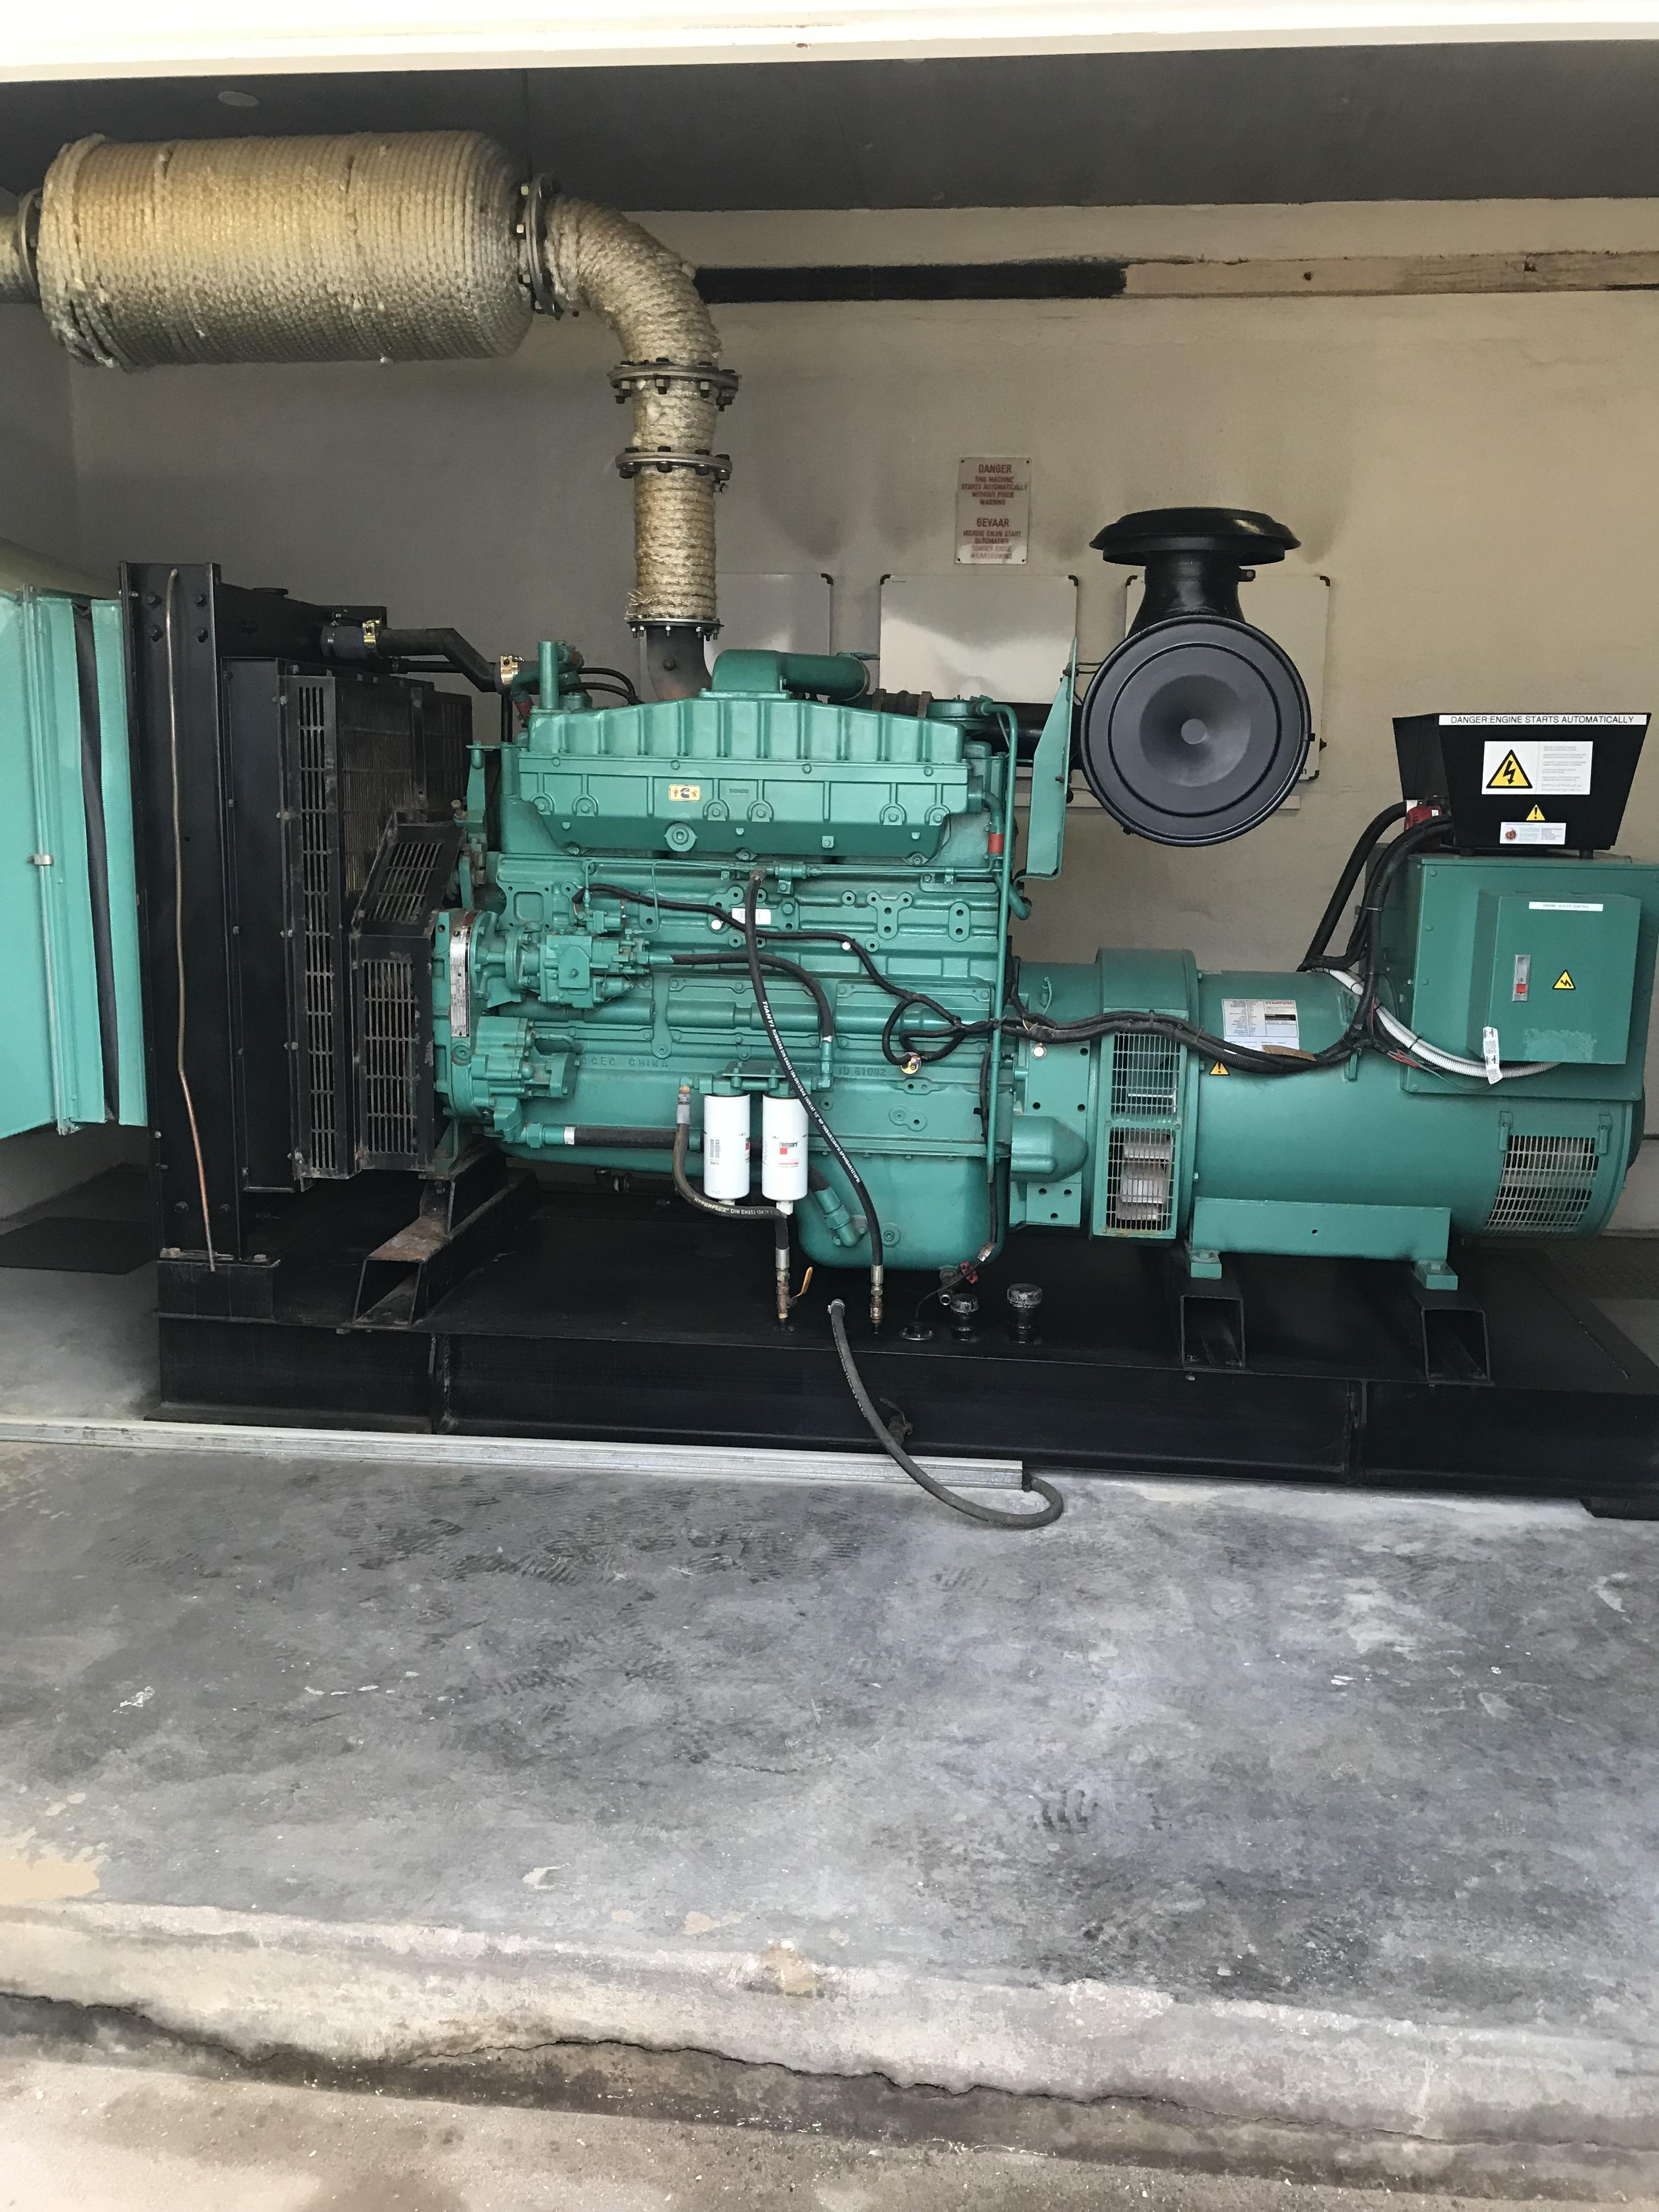
\includegraphics[width=0.5\textwidth,height=\textheight]{images/generator/generator2.jpg}

}

\caption{\label{fig-generator}The National Marine Research and
Information Center back-up generator.}

\end{figure}

\hypertarget{generator-test}{%
\section{Generator Test}\label{generator-test}}

{The testing procedure described for the back-up generator (referred to
as the ``Generator'' throughout) should be done once a month}. {This can
be done by one competent person}. {It is important to inform Mr.~Chris
Bartholomae, who will inform the rest of the MFMR staff, prior to
testing the Generator}

\hypertarget{sec-gen-inspect}{%
\subsection{Generator inspection}\label{sec-gen-inspect}}

{Use the wall opposite the room entrance as a reference point when
following instructions regarding specific parts of the Generator, such
that you are facing the generator with your back to that wall}
(Figure~\ref{fig-mount-heat}).

\begin{figure}[H]

{\centering 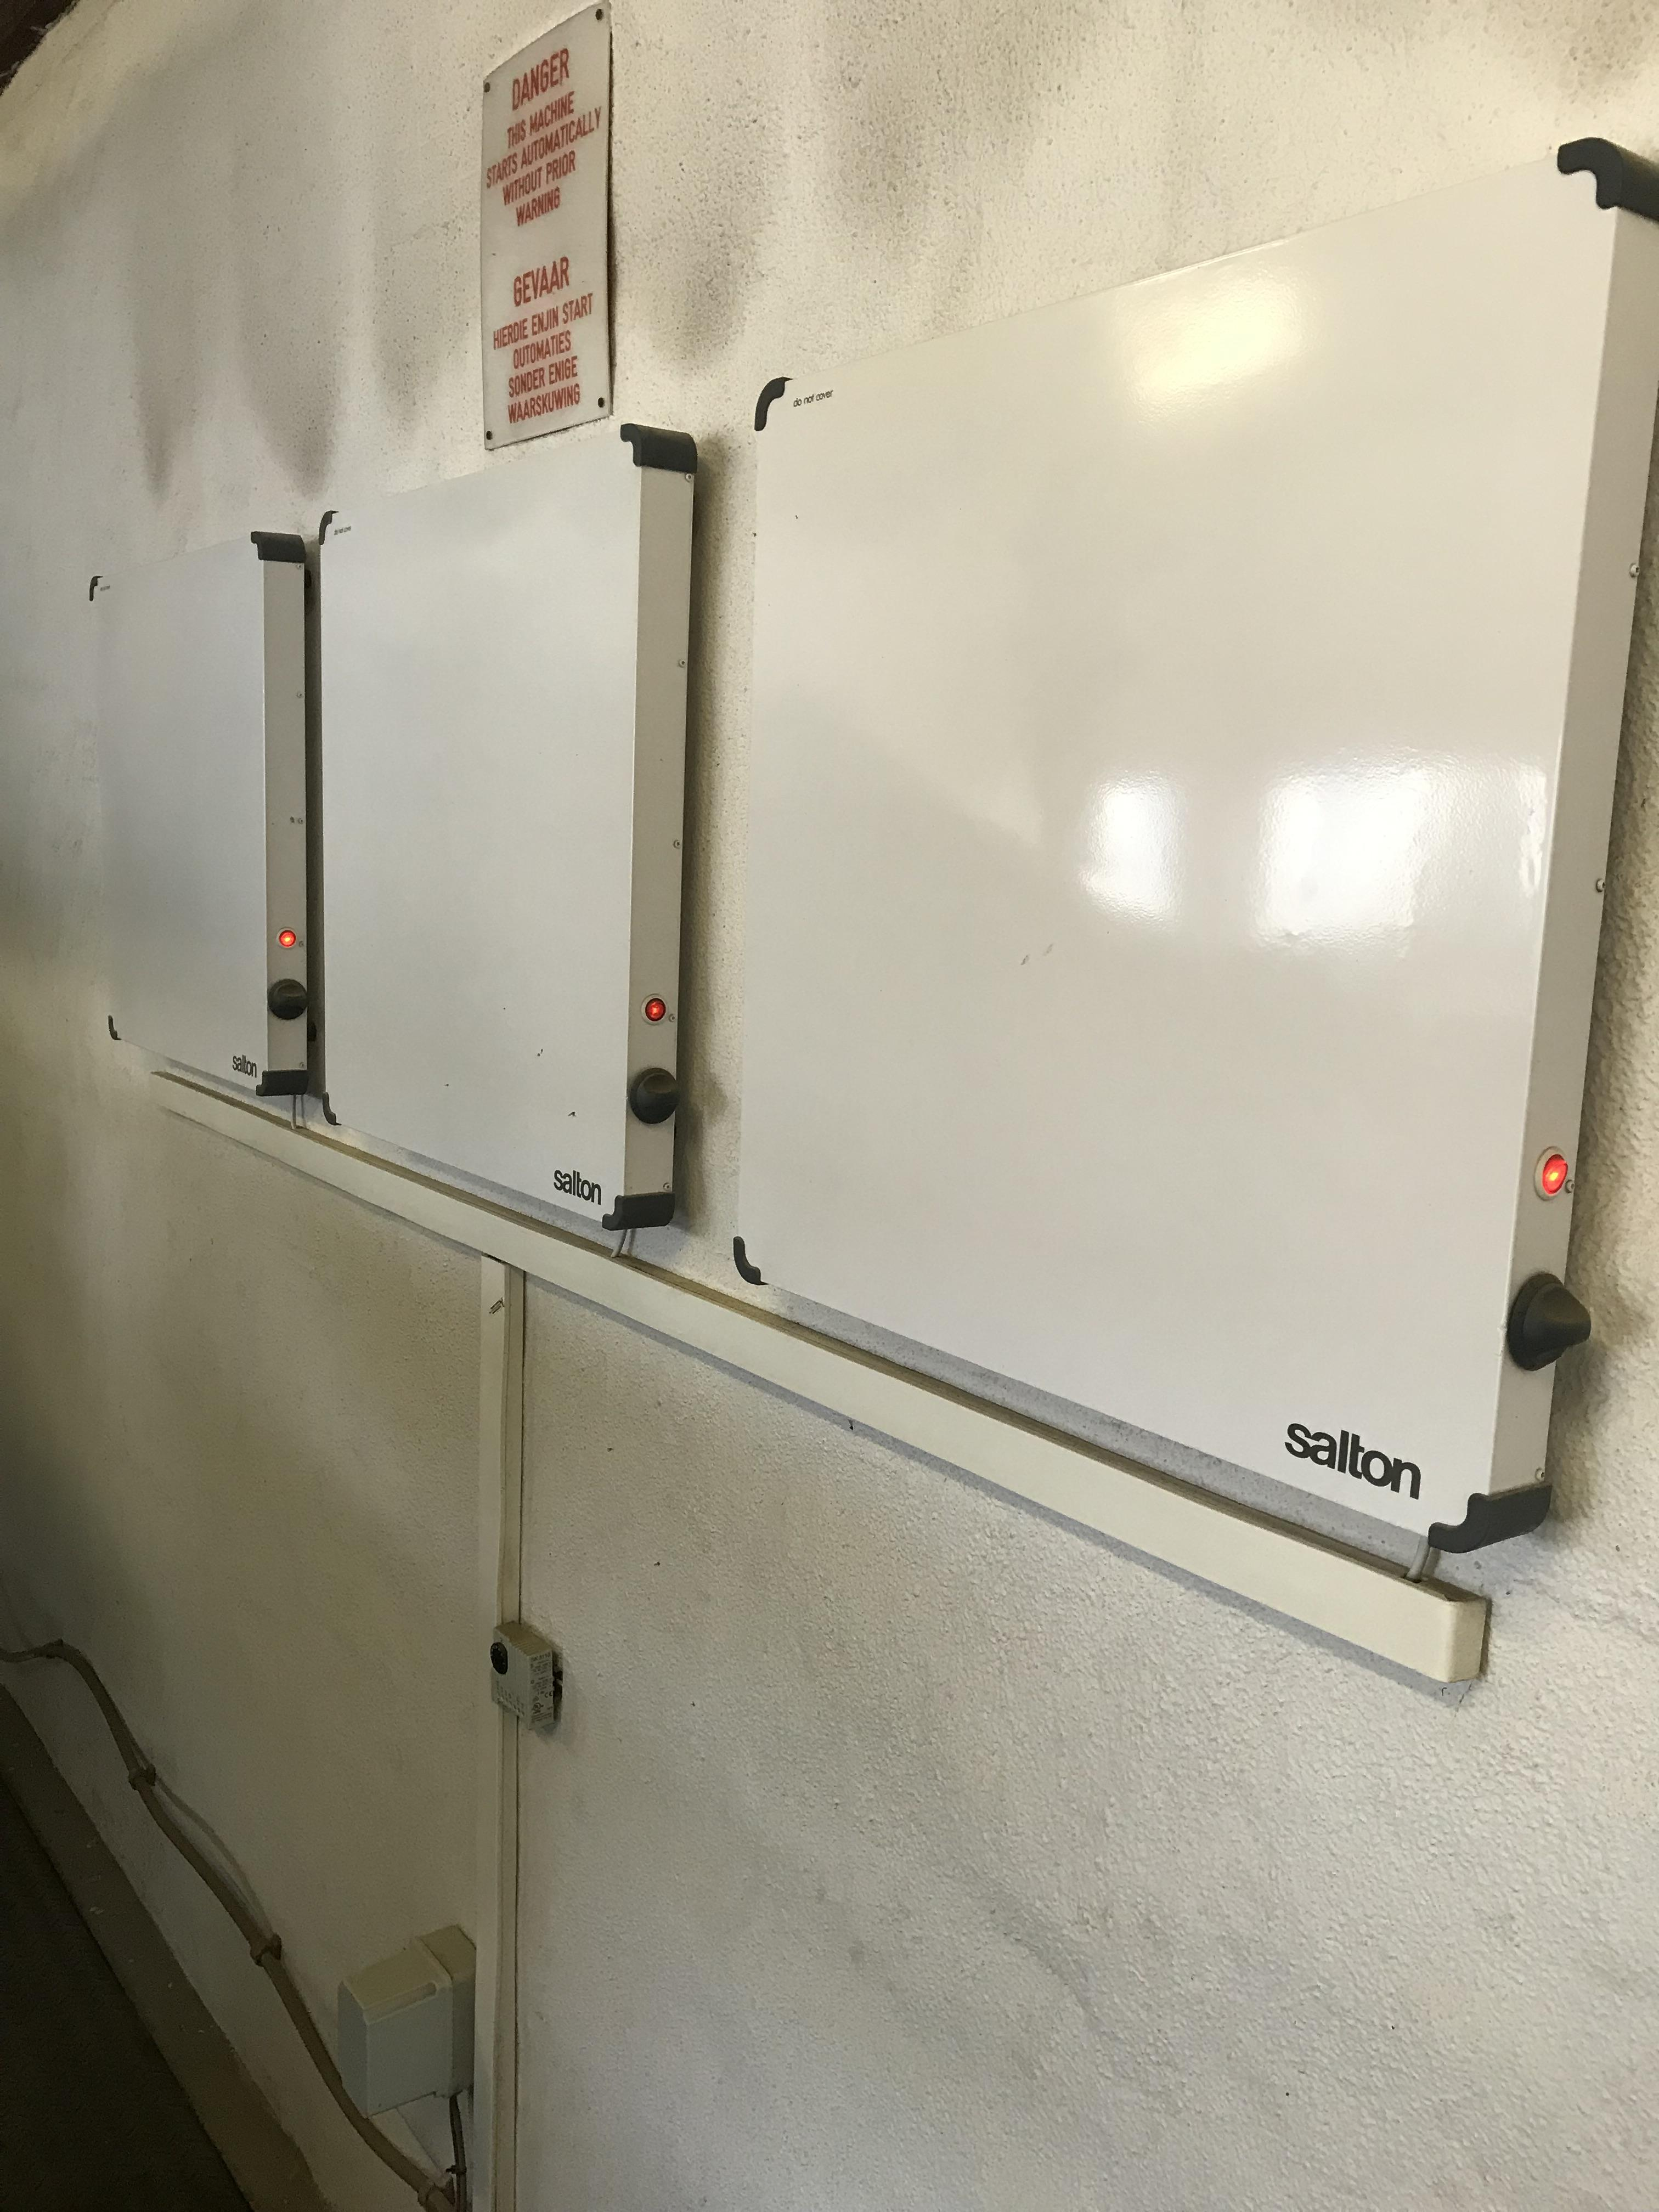
\includegraphics[width=0.5\textwidth,height=\textheight]{images/generator/mount_heat2.jpg}

}

\caption{\label{fig-mount-heat}Heaters mounted on the wall behind the
generator.}

\end{figure}

This is a quick inspection to ensure the Generator has enough essential
materials for the test e.g., oil and water. Most of the inspection
points can be found around the back of the Generator.

\begin{enumerate}
\def\labelenumi{\arabic{enumi}.}
\tightlist
\item
  Check the oil level (Figure~\ref{fig-gen-dipstick}).

  \begin{itemize}
  \tightlist
  \item
    \emph{This can be done by pulling out the dipstick near the bottom
    of the tank, along its' lateral axis}.
  \item
    \emph{If oil levels are low, the generator can be filled with spare
    oil from the Diesel tank storage (Room 11)}.
  \end{itemize}
\item
  Look for any major oil leaks beneath the oil sump
  (Figure~\ref{fig-gen-sump}).

  \begin{itemize}
  \tightlist
  \item
    \emph{Next to the dipstick}.
  \end{itemize}
\item
  Check the radiator water level (Figure~\ref{fig-radiator-cap}).

  \begin{itemize}
  \tightlist
  \item
    \emph{Found on the top right of the generator}.
  \item
    \emph{If the Radiator water level is low, refill it with fresh
    water}.
  \end{itemize}
\item
  Look for any water leaks around the Radiator.
\end{enumerate}

\begin{figure}[H]

\begin{minipage}[t]{0.33\linewidth}

{\centering 

\raisebox{-\height}{

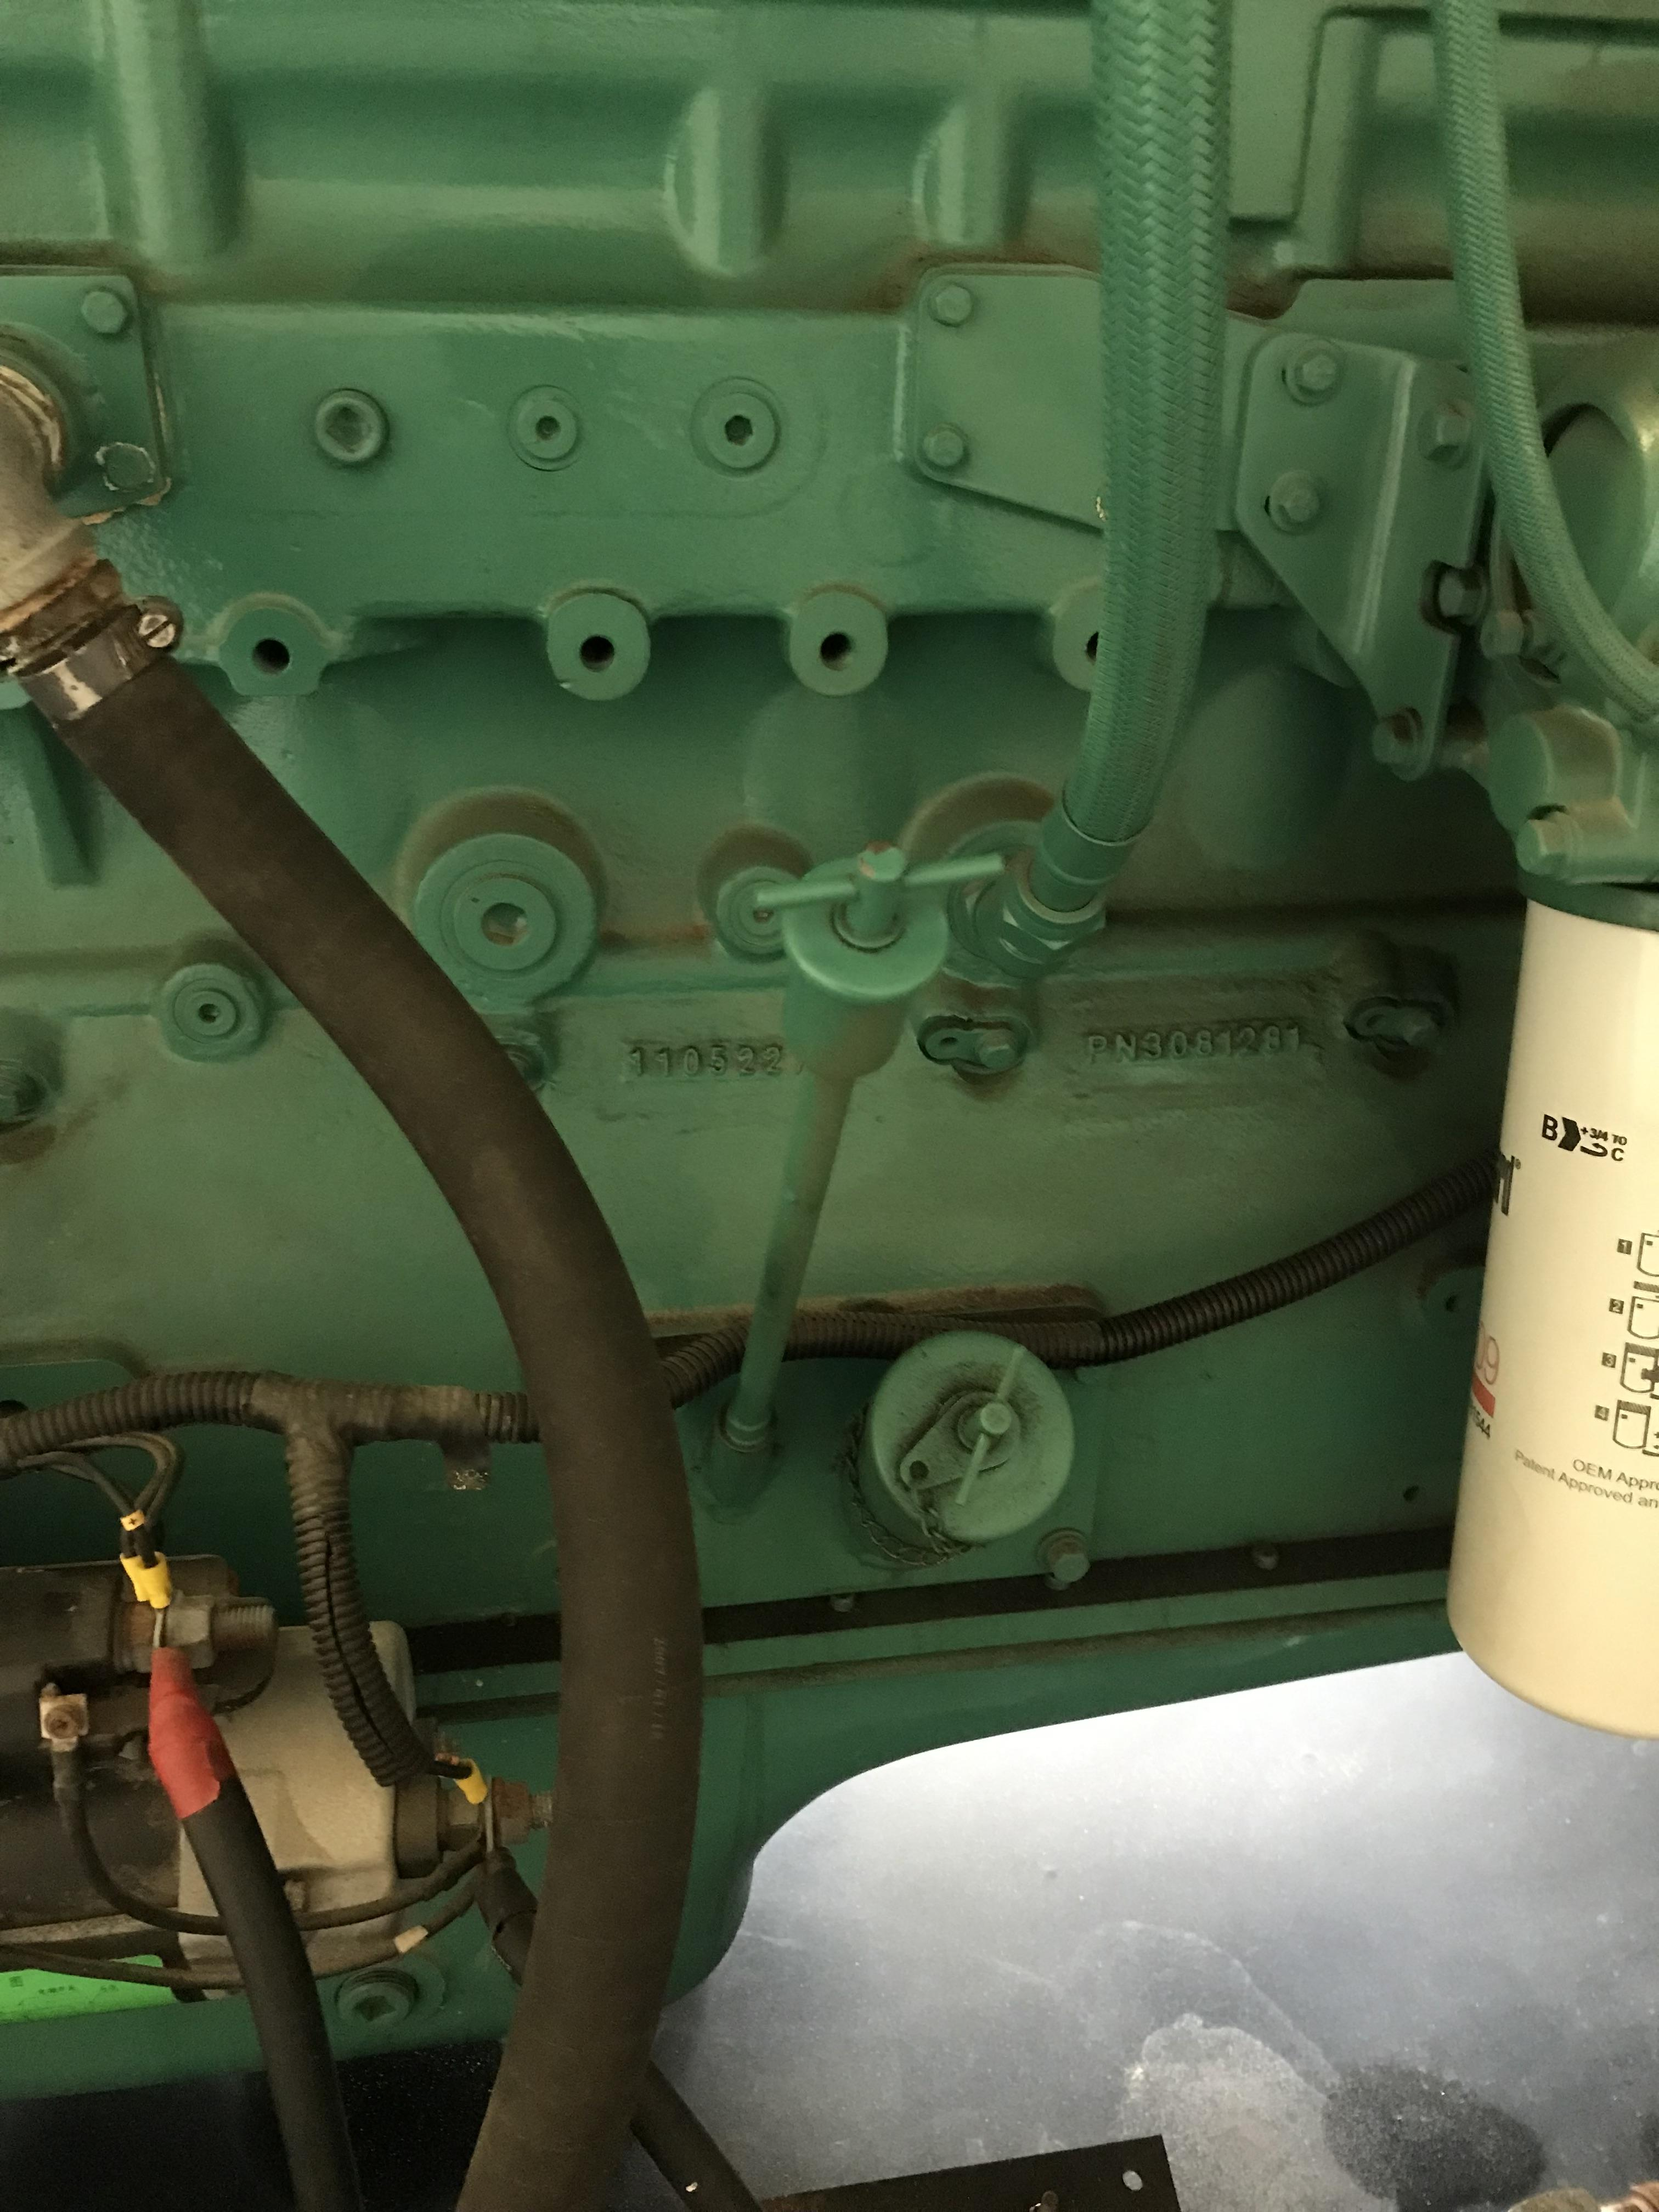
\includegraphics{images/generator/gen_dipstick2.jpg}

}

}

\subcaption{\label{fig-gen-dipstick}Oil dipstick}
\end{minipage}%
%
\begin{minipage}[t]{0.33\linewidth}

{\centering 

\raisebox{-\height}{

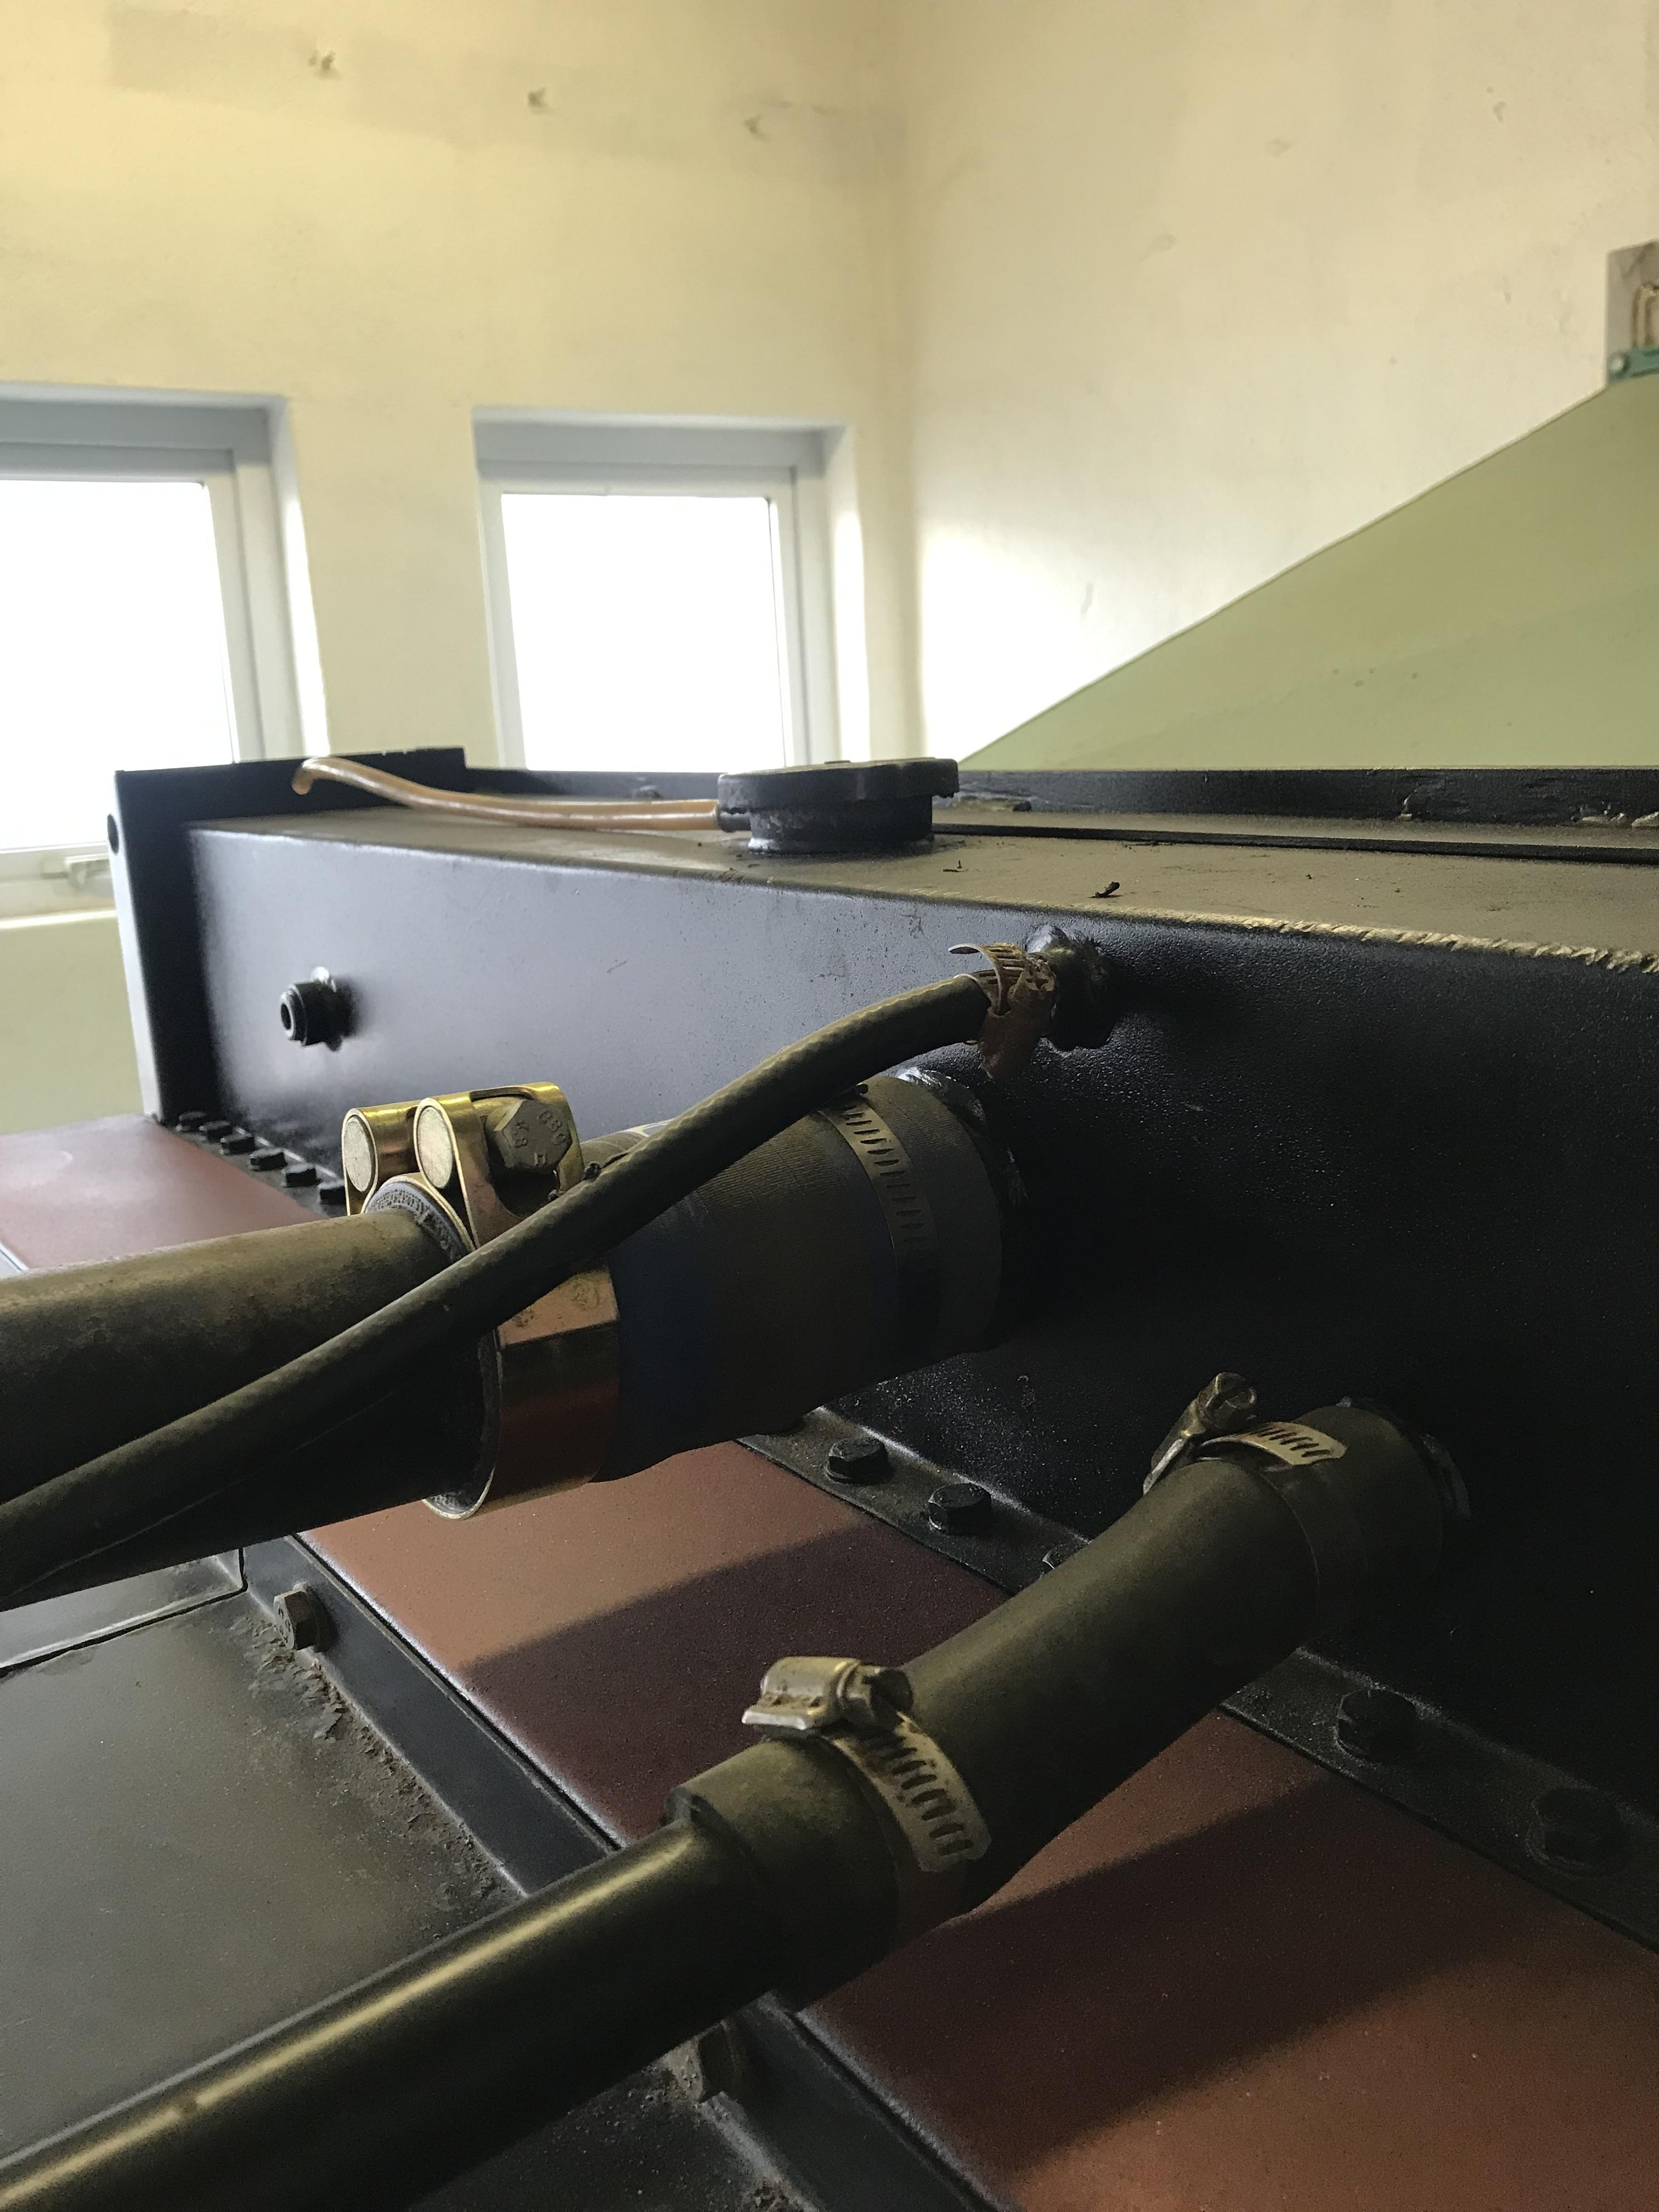
\includegraphics{images/generator/radiator2.jpg}

}

}

\subcaption{\label{fig-radiator-cap}Radiator top cap}
\end{minipage}%
%
\begin{minipage}[t]{0.33\linewidth}

{\centering 

\raisebox{-\height}{

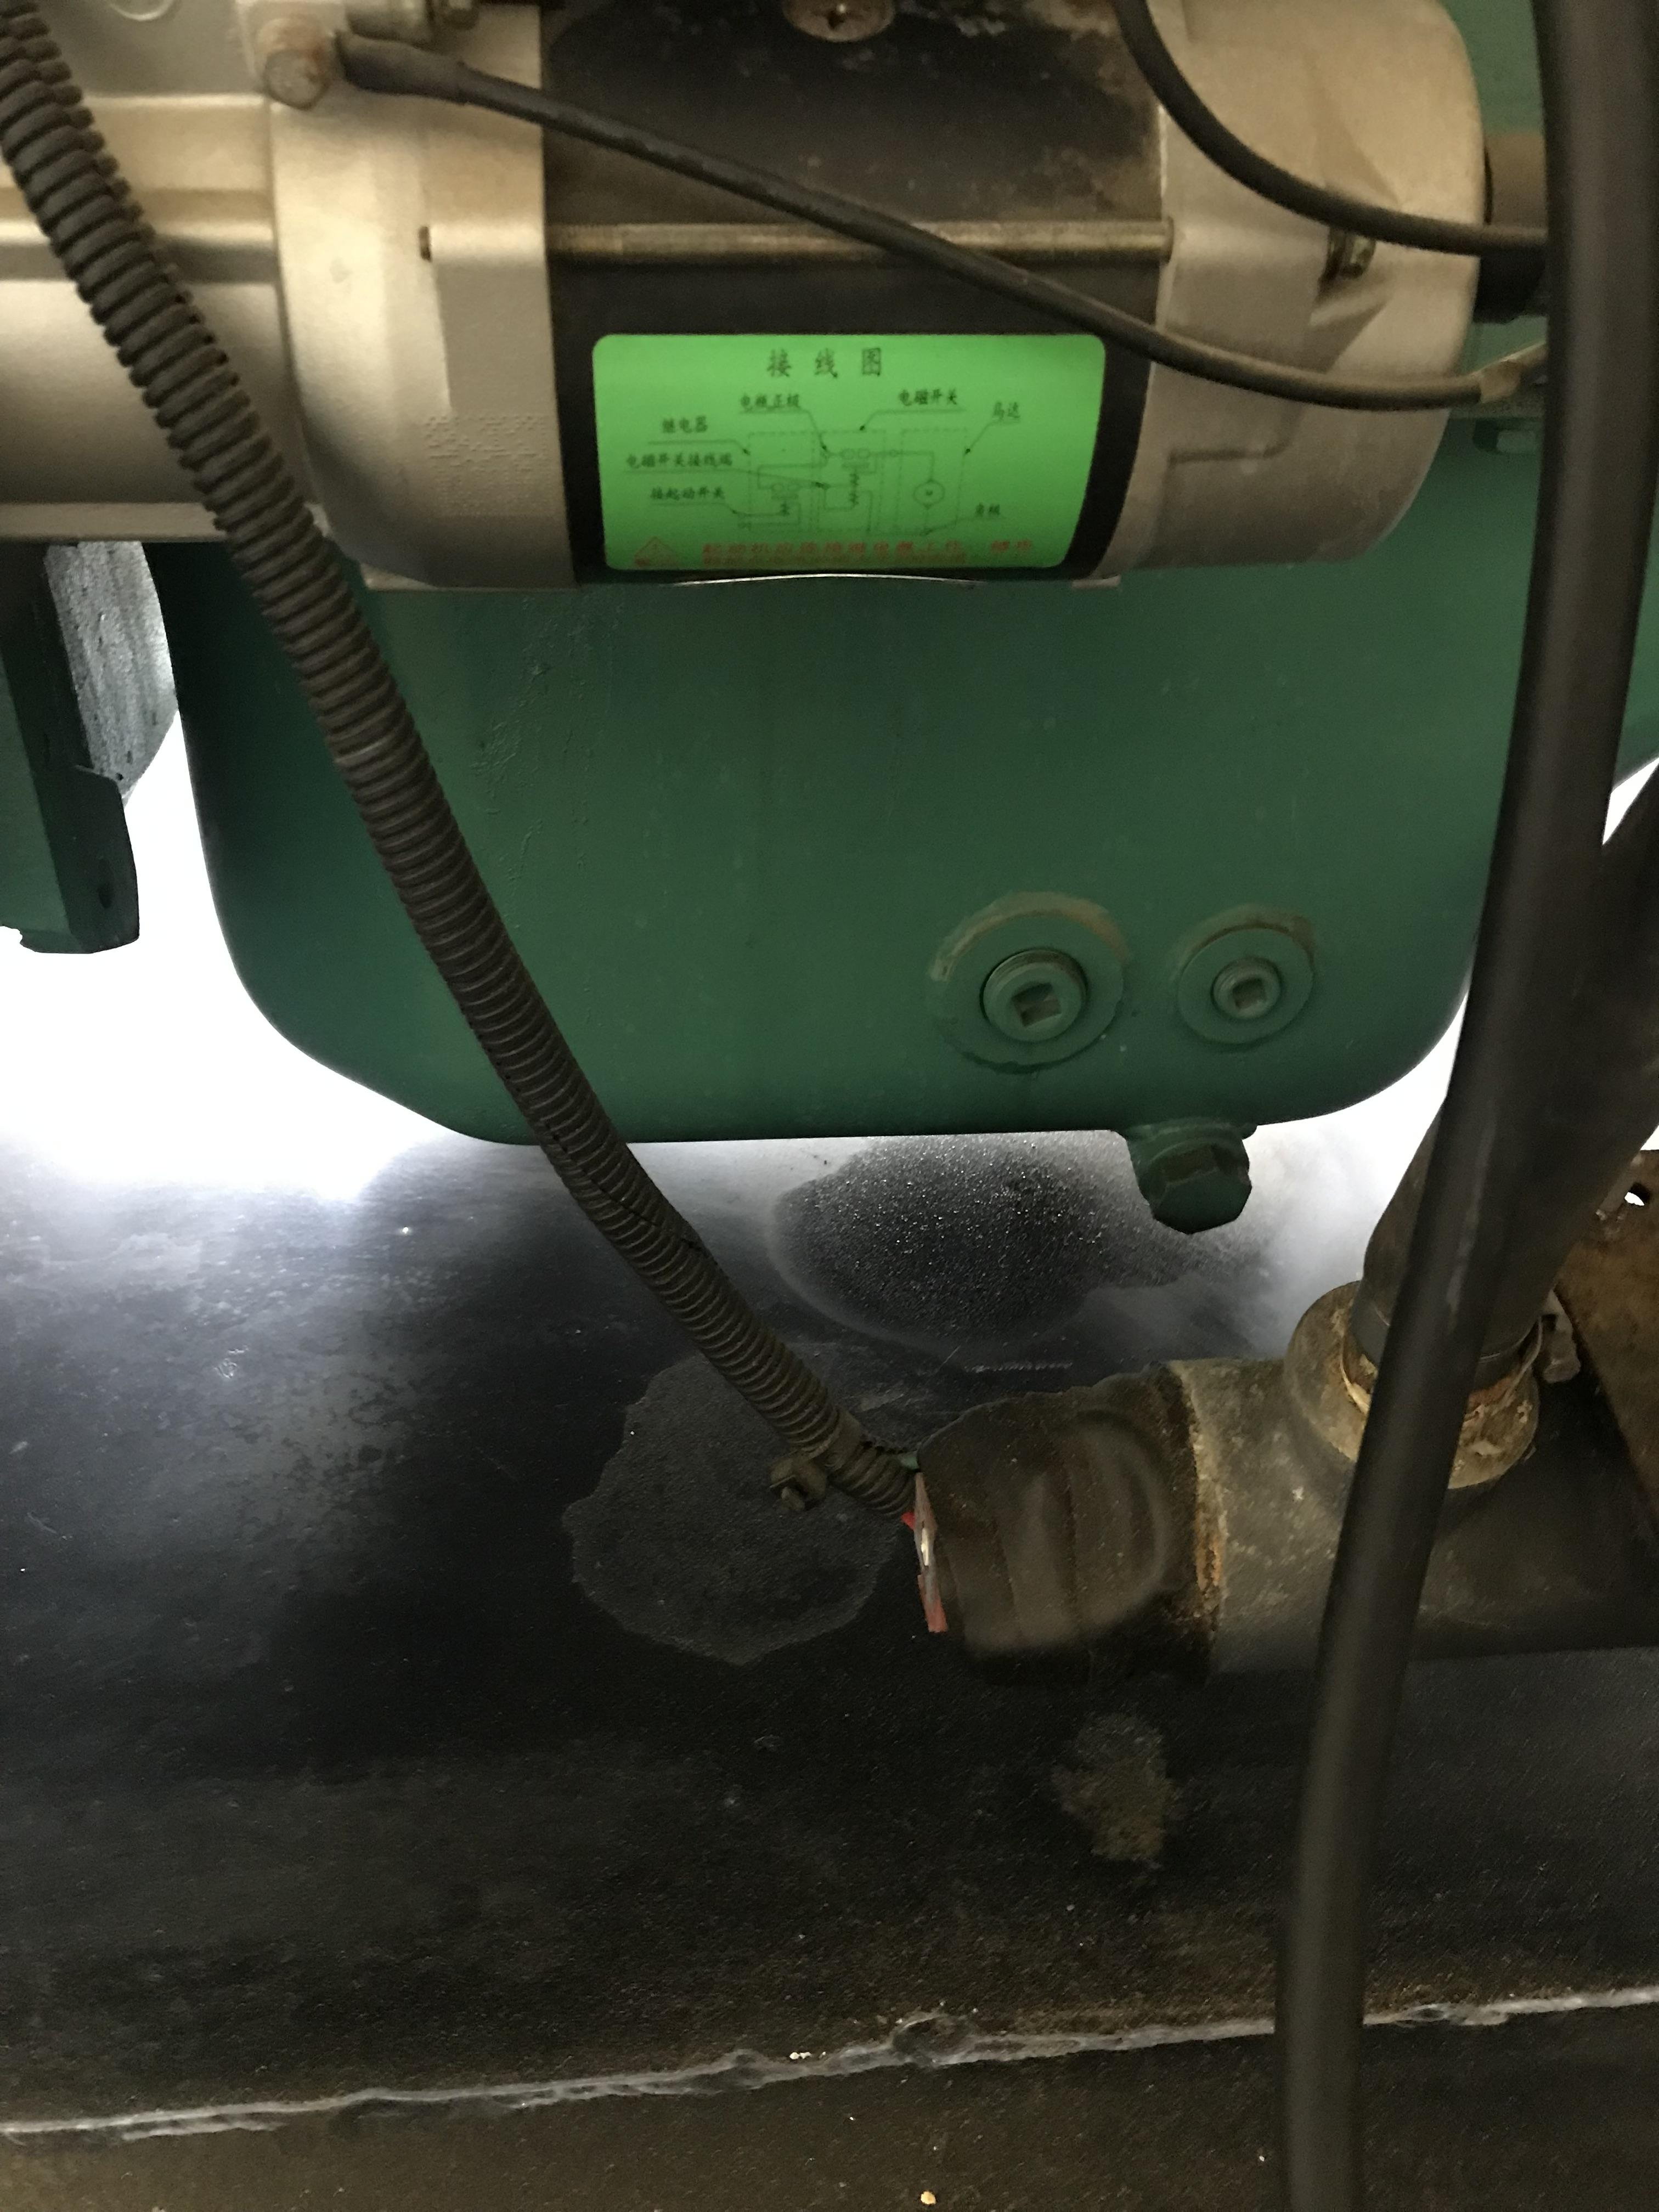
\includegraphics{images/generator/gen_sump2.jpg}

}

}

\subcaption{\label{fig-gen-sump}Oil sump}
\end{minipage}%

\caption{\label{fig-generator}Different points of interest around the
back of the generator, which have to be inspected during the testing
procedure.}

\end{figure}

\begin{enumerate}
\def\labelenumi{\arabic{enumi}.}
\setcounter{enumi}{4}
\tightlist
\item
  Make sure the heaters on the back wall are turned on
  ((Figure~\ref{fig-mount-heat})).

  \begin{itemize}
  \tightlist
  \item
    \emph{This ensures moisture does not condense around any essential
    parts of the generator}.
  \end{itemize}
\end{enumerate}

\hypertarget{sec-gen-test}{%
\subsection{Generator test}\label{sec-gen-test}}

\begin{enumerate}
\def\labelenumi{\arabic{enumi}.}
\setcounter{enumi}{5}
\tightlist
\item
  Turn off the Main power switch (Figure~\ref{fig-main-switch}).

  \begin{itemize}
  \tightlist
  \item
    \emph{Found in Room 10a (Main electrical control units and
    Distribution board) next to the Generator room}
    (Figure~\ref{fig-main-power-room}).
  \item
    \emph{First switch on the left most distribution board}.
  \end{itemize}
\end{enumerate}

\begin{figure}[H]

\begin{minipage}[t]{0.50\linewidth}

{\centering 

\raisebox{-\height}{

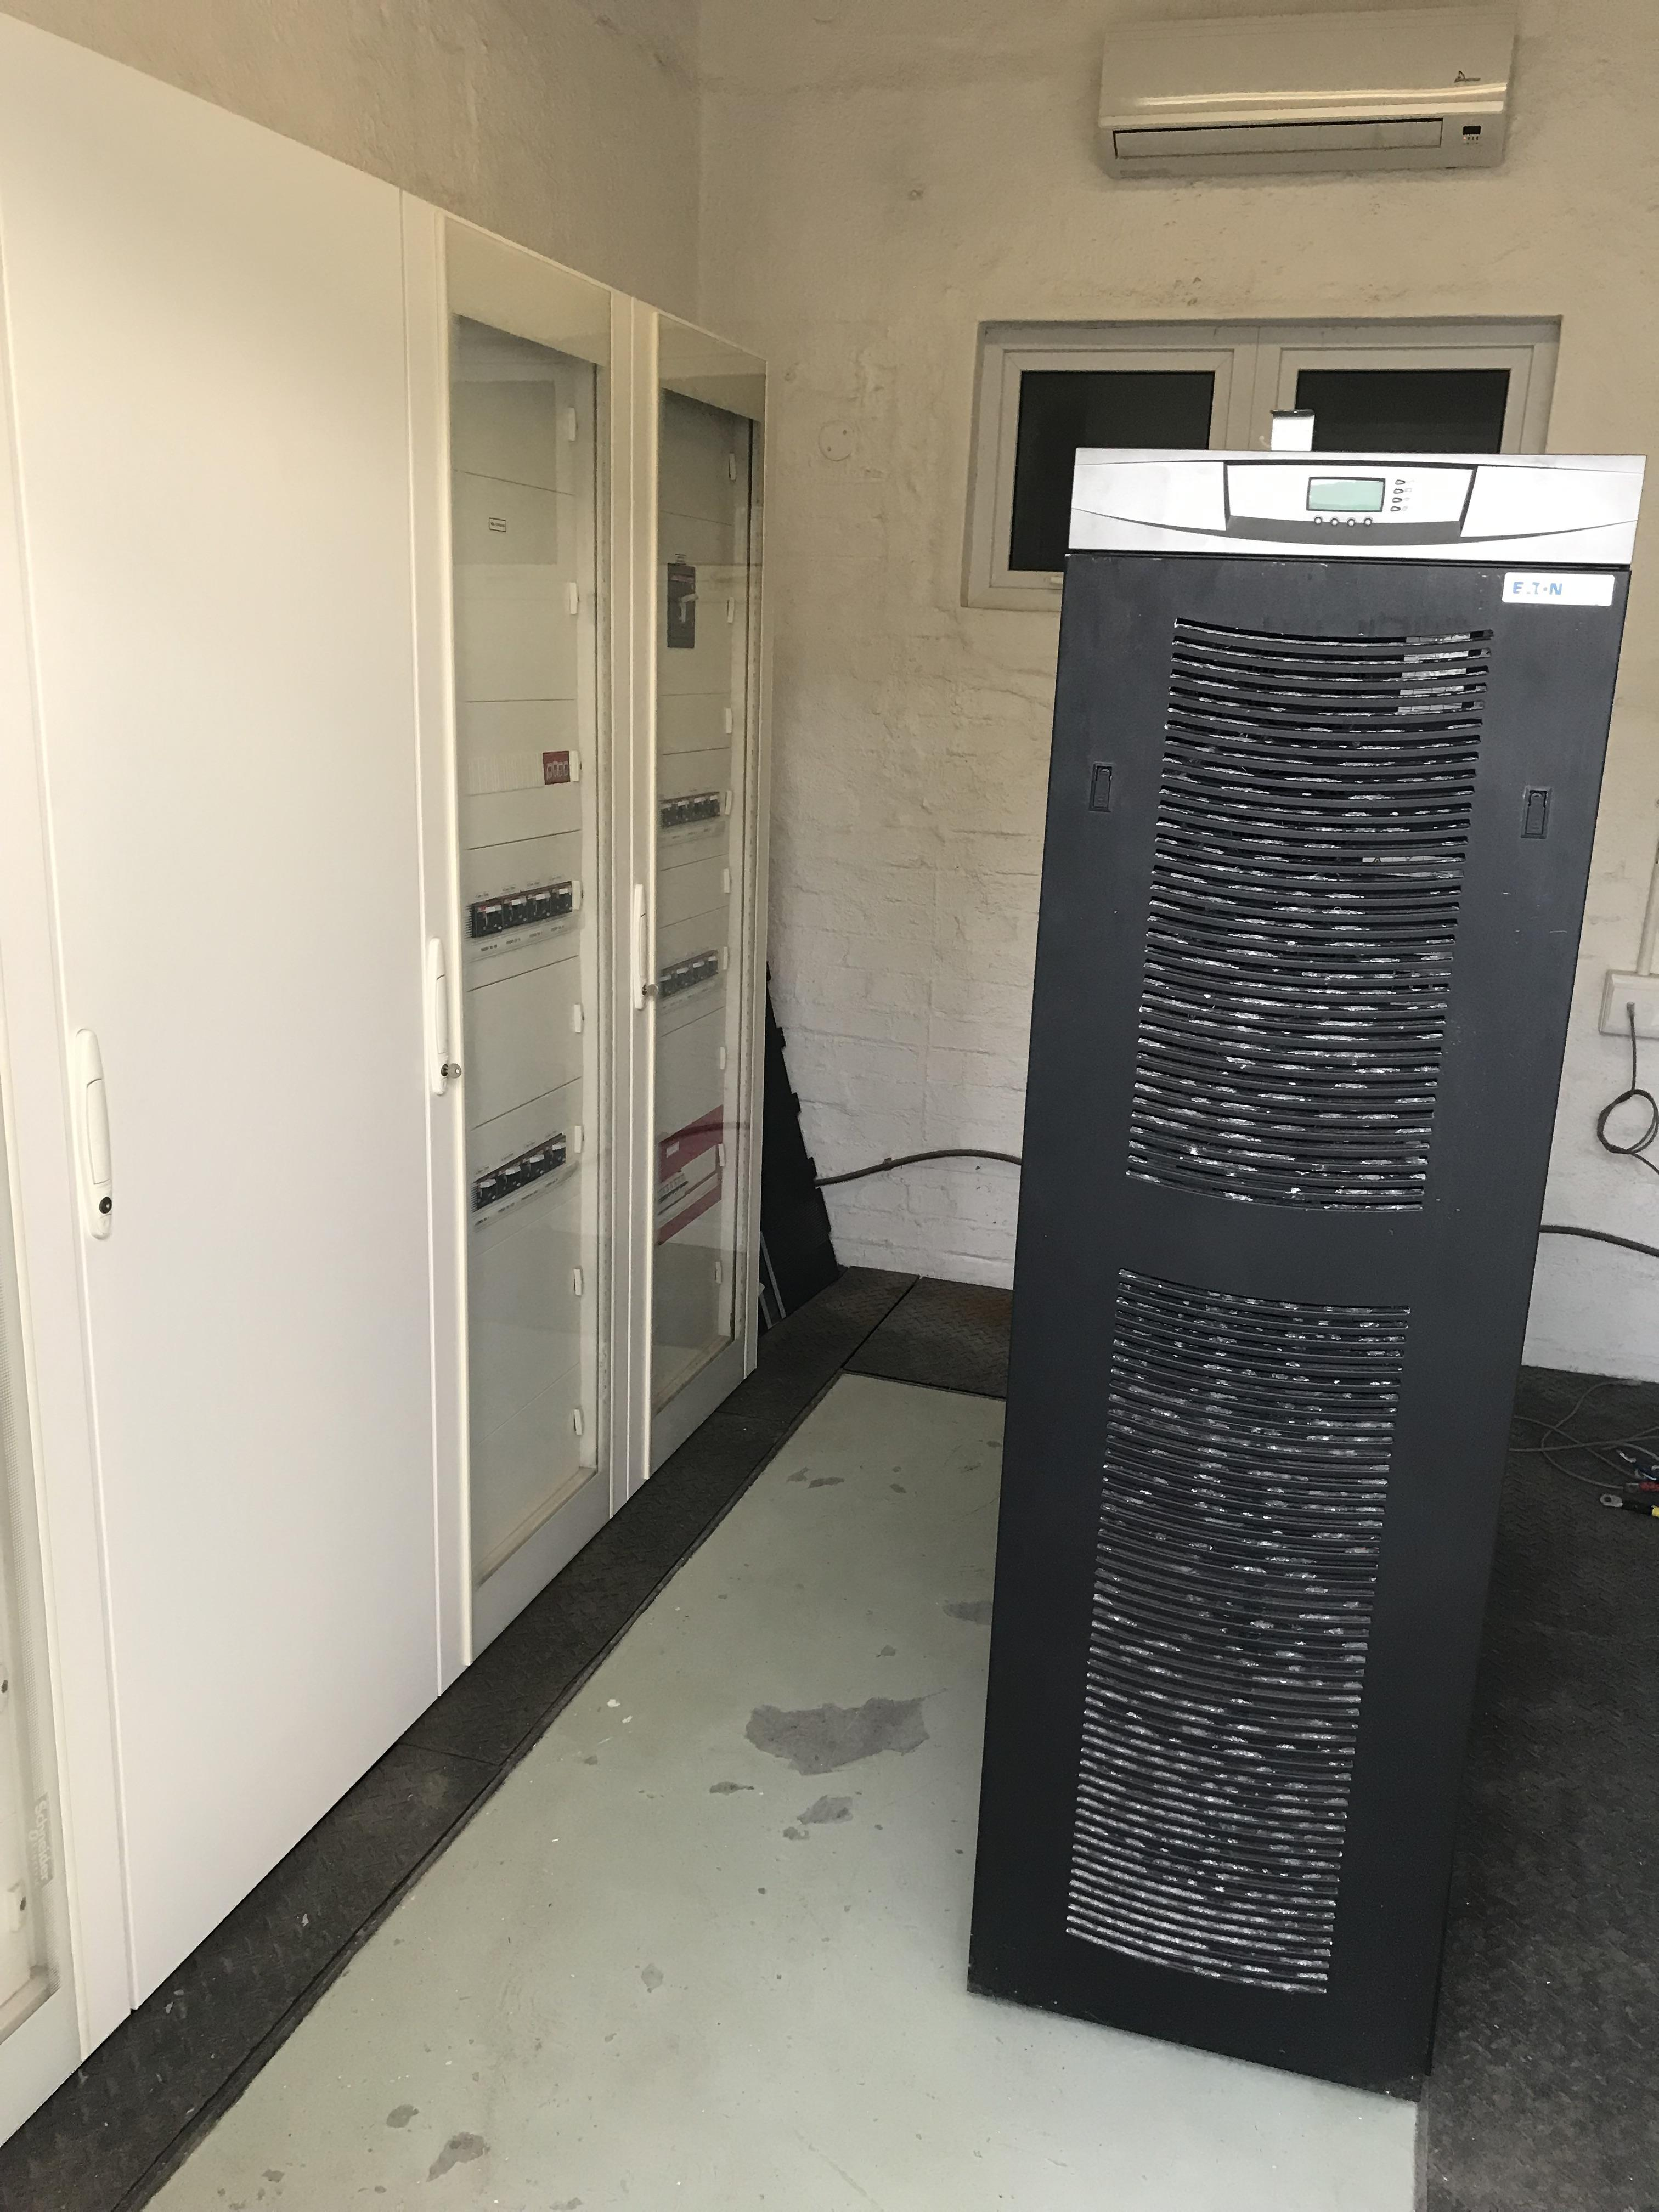
\includegraphics{images/generator/main_proom2.jpg}

}

}

\subcaption{\label{fig-main-power-room}Main power distribution room}
\end{minipage}%
%
\begin{minipage}[t]{0.50\linewidth}

{\centering 

\raisebox{-\height}{

\includegraphics{images/generator/main_switch2.jpg}

}

}

\subcaption{\label{fig-main-switch}Main power switch (left)}
\end{minipage}%

\caption{\label{fig-mains-comp}The main power supply switch for NATMiRC
found in room 10a.}

\end{figure}

\begin{enumerate}
\def\labelenumi{\arabic{enumi}.}
\setcounter{enumi}{6}
\tightlist
\item
  The Generator will start automatically after approximately 1 minute.

  \begin{itemize}
  \tightlist
  \item
    \emph{The Jetty pump will switch off, triggering the ``Raw water no
    flow'' alarm}.
  \item
    \emph{Filter pump 1 will switch off and back on again, triggering
    the ``Filter pump 1 stop'' alarm}.
  \item
    \emph{Leave the Generator on for one hour}.
  \end{itemize}
\end{enumerate}

\begin{itemize}
\tightlist
\item
  \textbf{Steps 8, 9, 14 and 15 will be completed using the Plant rooms'
  Main control switchboard} (Figure~\ref{fig-mcs}).
\end{itemize}

\begin{enumerate}
\def\labelenumi{\arabic{enumi}.}
\setcounter{enumi}{7}
\tightlist
\item
  Press the Reset button to turn the Jetty pump back on.
\item
  Press the Alarm cancel button.
\item
  After one hour, turn the Main power switch back on
  (Figure~\ref{fig-main-switch}).

  \begin{itemize}
  \tightlist
  \item
    \emph{All alarms raised in step 5 will be triggered again}
  \end{itemize}
\item
  Look for any new oil leaks beneath the oil sump.
\item
  Look for any new water leaks around the Radiator.
\item
  Inspect the Generators' digital display board or simply the display
  board (Figure~\ref{fig-gen-display}).

  \begin{itemize}
  \tightlist
  \item
    \emph{Found on the right of the Generator}.
  \item
    \emph{Press any of the direction keys to start navigating the
    display board}.
  \item
    \emph{Stop at ``Engine instruments'' to find run times, fuel levels,
    etc}.
  \end{itemize}
\end{enumerate}

\begin{figure}[H]

{\centering 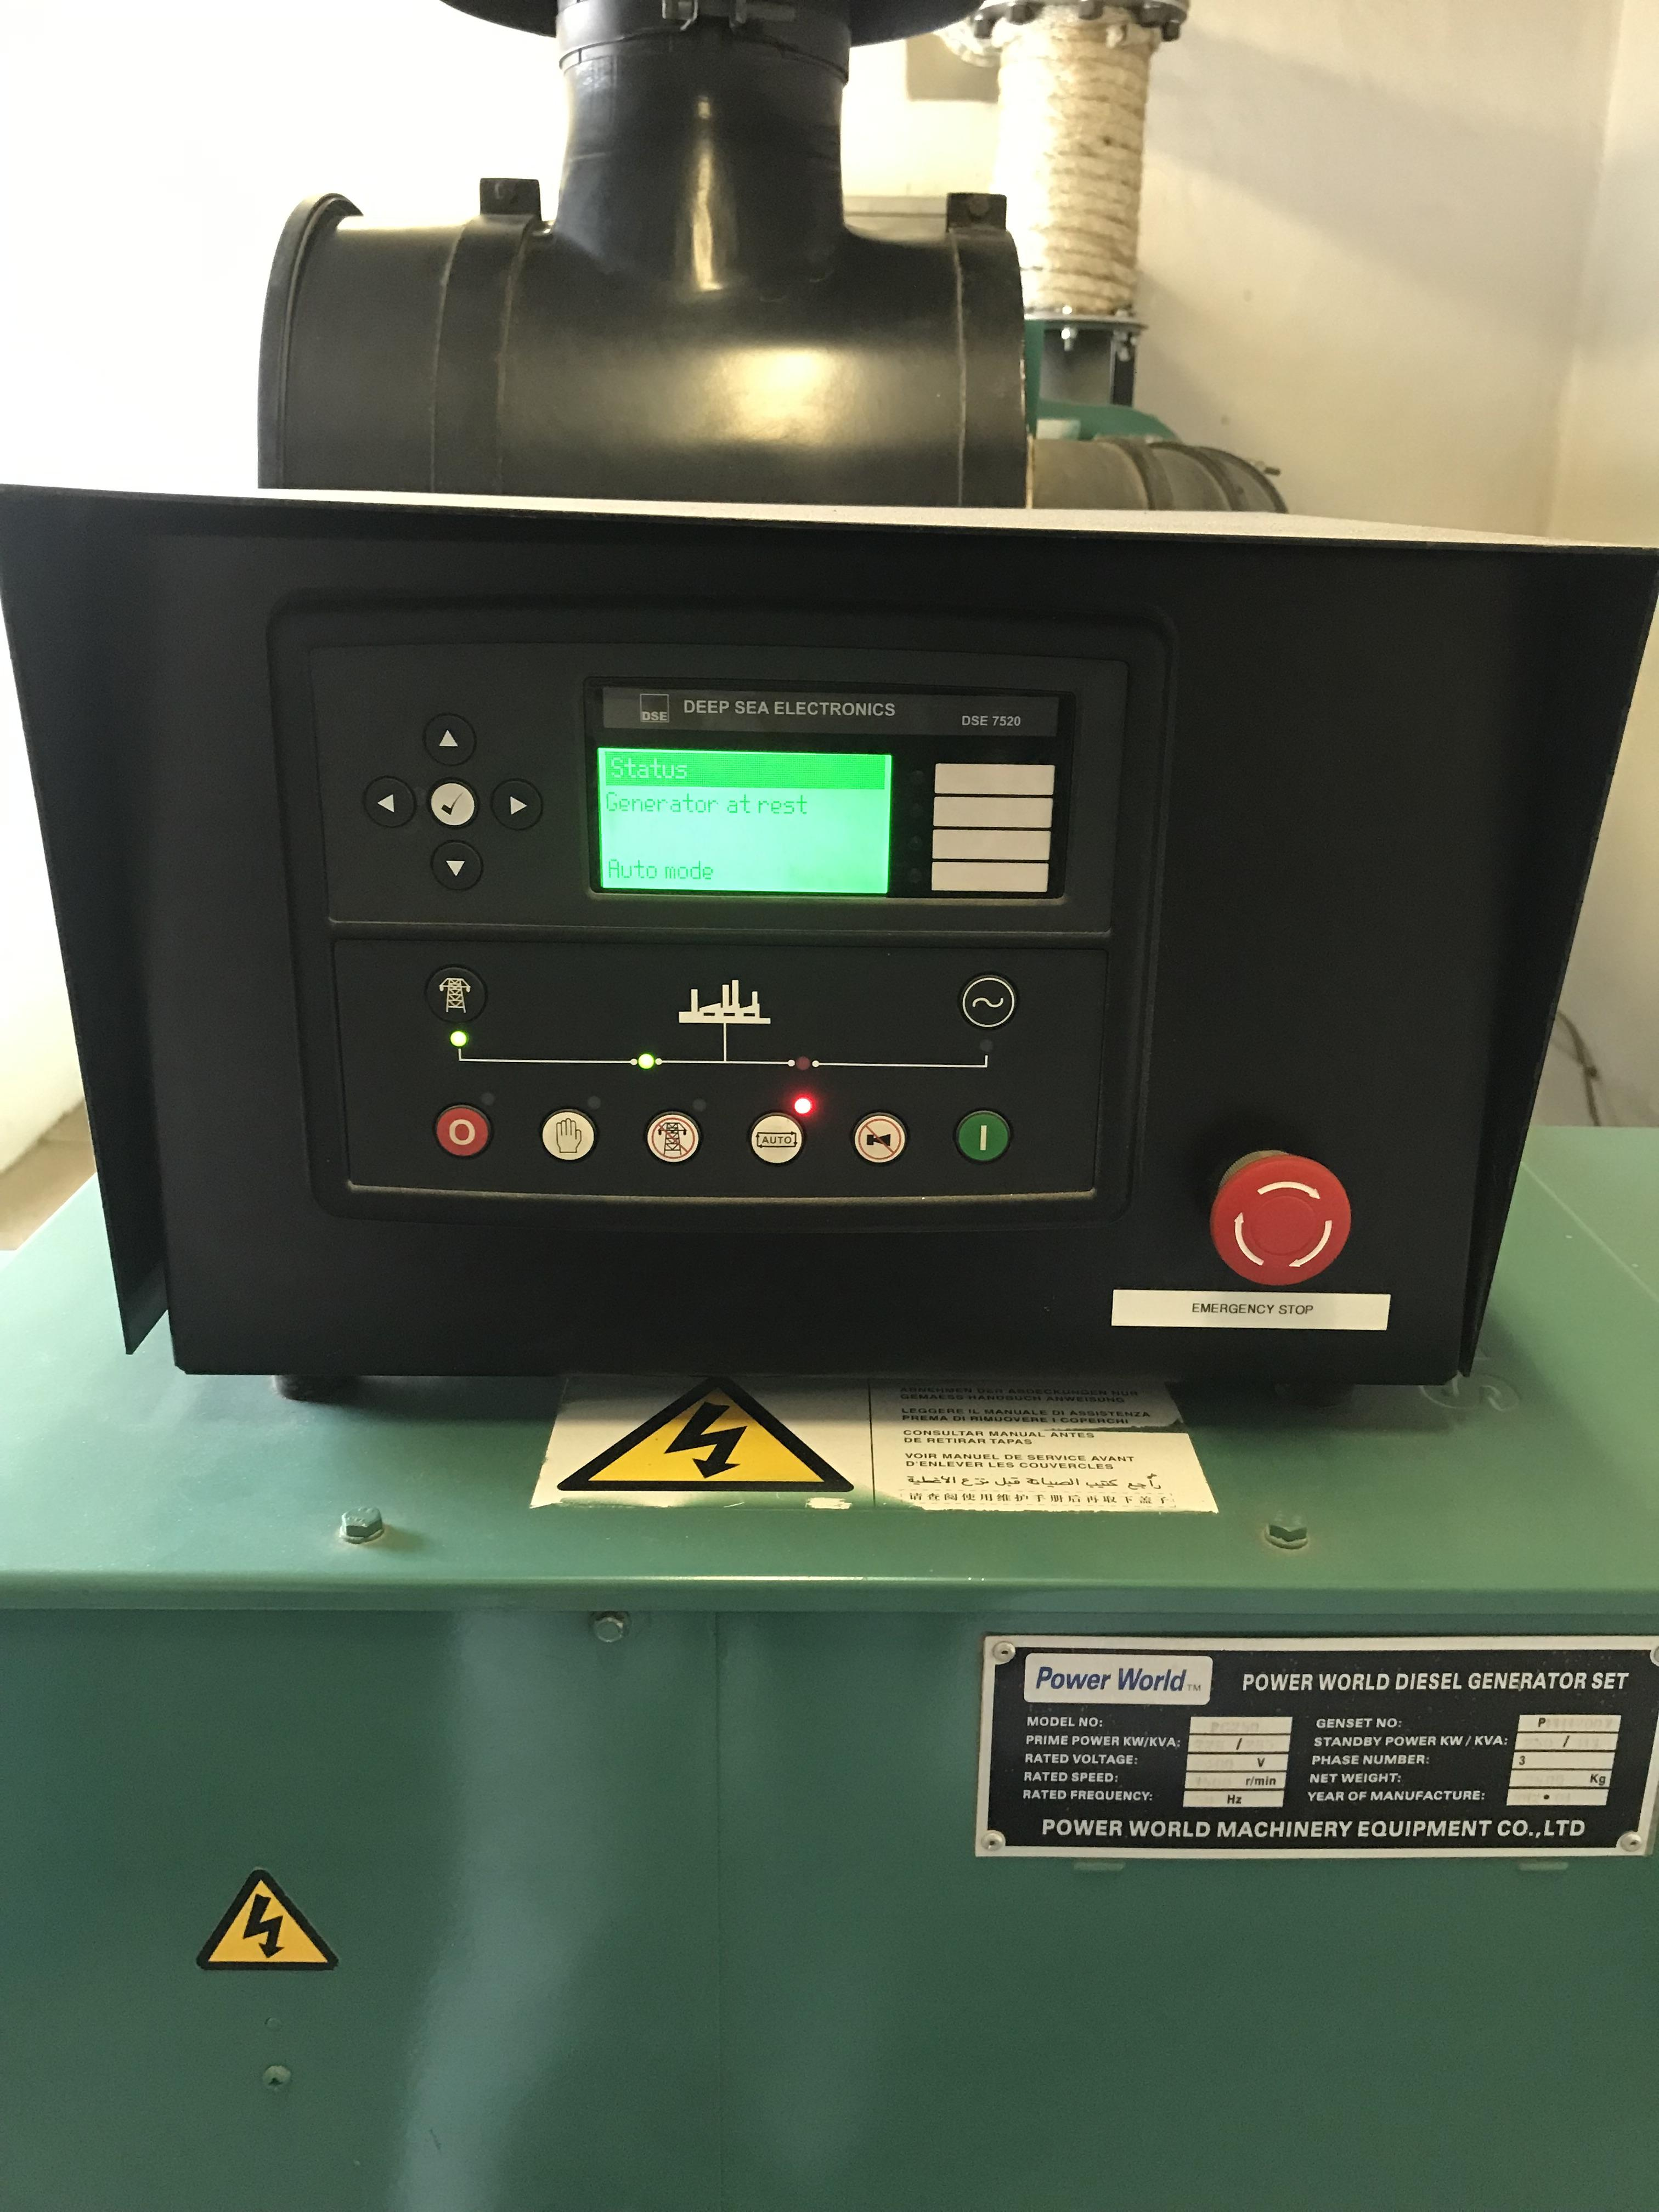
\includegraphics[width=0.5\textwidth,height=\textheight]{images/generator/gen_display2.jpg}

}

\caption{\label{fig-gen-display}The generator's information display
panel, mounted on it's right side.}

\end{figure}

\begin{enumerate}
\def\labelenumi{\arabic{enumi}.}
\setcounter{enumi}{13}
\tightlist
\item
  Press the Reset button to turn the Jetty pump back on
  (Figure~\ref{fig-mcs}).
\item
  Press the Alarm cancel button.
\end{enumerate}

\hypertarget{refuel-diesel-storage-tank}{%
\section{Refuel Diesel storage tank}\label{refuel-diesel-storage-tank}}

The Diesel storage tank (referred to as the ``Diesel tank'' throughout)
can be found in the Diesel storage room (Nr. 11), between the MFMR
garage and the Generator room. It has a 2500\(l\) fuel storage capacity
and is normally refueled by one of MFMR's fuel suppliers e.g., Namcor or
Crossroads Caltex service station. There is a fuel line that feeds from
the Diesel tank, directly into the Generator's fuel tank.

\hypertarget{refuel-generator}{%
\section{Refuel Generator}\label{refuel-generator}}

The generator has a 1000\(l\) fuel tank at it's base, which only has to
be refueled once the fuel level drops below 40\%. This can be determined
by scrolling to the Generator's ``Engine instrumentation'' section in
the display board (Section???). Completing this procedure will require
access to both the Generator room and the Diesel storage room.

\hypertarget{sec-gen-fuel-tool}{%
\subsection{Tool preparation}\label{sec-gen-fuel-tool}}

\textbf{The required tools can be found inside the workshop (room 162),
in the generator room (Nr. 10a) or in the Diesel tank room (Nr. 11)}.

These include:

\begin{itemize}
\tightlist
\item
  1 x Pipe wrench
\item
  3 x Old buckets
\item
  1 x Old cloth 1 x Short hose pipe (approximately 2m long) 1 x Used 10
  m\(l\) Air cylinder

  \begin{itemize}
  \tightlist
  \item
    \emph{Remove the breather from it's air delivery line}. 1 x Small
    screw driver (Nr. 2)
  \end{itemize}
\end{itemize}

\hypertarget{prime-the-refuel-line}{%
\subsection{Prime the refuel line}\label{prime-the-refuel-line}}

Before refueling the Generator, it's fuel inlet line, from the Diesel
storage tank, has to be cleared of any blockages that may be caused by
dry fuel residue. This is done to prevent weak fuel flow, essentially
optimizing the time required to refuel the Generator tank.

{Atleast two technical Aquarium staff members (one in the Generator room
and the other in the Diesel storage room) are required to carry out this
procedure}

\begin{enumerate}
\def\labelenumi{\arabic{enumi}.}
\tightlist
\item
  Make sure the Diesel tank's outlet valve is closed.

  \begin{itemize}
  \tightlist
  \item
    \emph{Close it if it is open}.
  \end{itemize}
\item
  Place a bucket under the Diesel tank's, fuel outlet line, L-shaped
  connector found against the wall directly opposite the rooms entrance.
\item
  Disconnect the L-shaped pipe connector.

  \begin{itemize}
  \tightlist
  \item
    \emph{Loosen the threaded pipe screw with your fingers}.
  \item
    \emph{Some diesel might spill into the bucket}.
  \end{itemize}
\item
  Disconnect and remove the Generator's fuel inlet pipe from the fuel
  tank.

  \begin{itemize}
  \tightlist
  \item
    \emph{Done to monitor the pipe priming process from the opposite
    end}.
  \item
    \emph{Use the small screw driver to loosen the pipe clamp}.
  \end{itemize}
\item
  Drop the disconnected end of the pipe into a bucket.
\item
  Feed the Air cylinder's delivery line into the horizontal section of
  the Diesel tank's disconnected pipe.

  \begin{itemize}
  \tightlist
  \item
    \emph{Interested in blowing air towards the Generator tank's
    disconnected pipe end}.
  \end{itemize}
\end{enumerate}

\begin{itemize}
\tightlist
\item
  \textbf{The staff members should communicate before executing Steps 7
  and 9}.
\end{itemize}

\begin{enumerate}
\def\labelenumi{\arabic{enumi}.}
\setcounter{enumi}{6}
\tightlist
\item
  Open the cylinder's outlet valve.

  \begin{itemize}
  \tightlist
  \item
    \emph{Hold the delivery line in place}.
  \item
    \emph{Diesel will shoot out at the other end of the pipe and into
    the bucket}.
  \end{itemize}
\item
  Leave the valve open until only air is discharged at the other end.
\item
  Close the outlet valve.
\item
  Remove the cylinder's air delivery pipe from the horizontal section of
  the Diesel tank's disconnected pipe.
\item
  Reconnect the L-shaped pipe connector.
\end{enumerate}

\begin{itemize}
\tightlist
\item
  \textbf{Contact one of the MFMR fuel suppliers (Section???) to help
  discard the fuel that has accumulated in the buckets (Steps 12 and
  14)}.
\end{itemize}

\begin{enumerate}
\def\labelenumi{\arabic{enumi}.}
\setcounter{enumi}{11}
\tightlist
\item
  Pack the bucket where it was found.
\item
  Clamp the Generator's fuel inlet pipe to the fuel tank.
\item
  Pack the bucket where it was found.
\end{enumerate}

\hypertarget{refuel-procedure}{%
\subsection{Refuel procedure}\label{refuel-procedure}}

{One technical Aquarium staff member required to carry out this
procedure}

\begin{enumerate}
\def\labelenumi{\arabic{enumi}.}
\setcounter{enumi}{14}
\tightlist
\item
  Note the Generator's fuel level (Section???)

  \begin{itemize}
  \tightlist
  \item
    \emph{If the fuel level \textgreater{} 40\% there is no need to
    proceed with this procedure}.
  \end{itemize}
\item
  Note the Diesel storage tanks fuel level (Section???).

  \begin{itemize}
  \tightlist
  \item
    \emph{If there is very little or no fuel left, this tank will have
    to be refueled before refueling the Generator (Section ???)}.
  \end{itemize}
\item
  Loosen the Diesel tank's filler cap.

  \begin{itemize}
  \tightlist
  \item
    \emph{Found on the top of the Diesel tank (climb on one of the oil
    barrels to the right to access it)}.
  \item
    \emph{Use the pipe wrench}.
  \item
    \emph{Done to ensure a vacuum is not created when the fuel levels
    drop in the Diesel tank}.
  \item
    \emph{Fuel will stop flowing from the tank if this is not done}.
  \end{itemize}
\item
  Loosen both of the Generator tank's filler caps.

  \begin{itemize}
  \tightlist
  \item
    \emph{Found on top of the Generator's fuel tank, on it's front end}.
  \item
    \emph{Use the pipe wrench}.
  \item
    \emph{Done to prevent pressure from building up in the tank, due to
    increasing fuel and diesel fume amounts}.
  \end{itemize}
\item
  Open both the Diesel tanks outlet valves.

  \begin{itemize}
  \tightlist
  \item
    \emph{Found at the tank's base, beneath the filler cap}.
  \end{itemize}
\item
  A bucket and hose pipe should be readily available, incase the fuel
  overflows.
\item
  Leave the Generator tank to fill up for an hour.
\item
  After one hour, return and note the Generator tank's fuel level
  (Section???).

  \begin{itemize}
  \tightlist
  \item
    \emph{This is used to determine the refuel rate, which will help
    provide an estimate for the total refuel time until 90\% of the
    Generator's capacity}.
  \end{itemize}
\item
  Leave the tank to continue filling up.
\item
  Return after the estimated total refuel time (Step 22).

  \begin{itemize}
  \tightlist
  \item
    \emph{90\% has been chosen as the refuel limit, leaving the extra
    10\% as a buffer against potential fuel spillage}.
  \end{itemize}
\item
  Check the Generator's fuel level.
\item
  Close the Diesel tank's outlet valves once the fuel level has reached
  90\%.

  \begin{itemize}
  \tightlist
  \item
    \emph{Can be slightly lower than 90\%}.
  \item
    \emph{This will stop the flow of fuel to the Generator tank}.
  \end{itemize}
\item
  Close the Diesel tank's filler cap.
\item
  Close the Generator tank's filler caps.
\item
  Note the Generator's fuel level (Section???).
\item
  The Generator's fuel level reading will fluctuate for a few days. Do
  not add more fuel.
\item
  Repack all tools in the correct storage rooms or compartments.
\end{enumerate}

\hypertarget{repairs-3}{%
\section{Repairs}\label{repairs-3}}

\textbf{If there is major damage to the Generator (see
Section~\ref{sec-gen-inspect} steps 2 and 4 and;
Section~\ref{sec-gen-test} steps 11 and 12), approach a reputable engine
rebuilder for help e.g., Namib Diesel (contact Mr.~Jaco de Witt)}.

{Read the report, \emph{Back-up generator repair} in the \emph{National
Marine Aquarium} folder, for a detailed description of the repair work
done on the Generators Radiator by Namib Diesel}.

\newpage

\hypertarget{procurement}{%
\chapter{Procurement}\label{procurement}}

\newpage

\hypertarget{transport}{%
\chapter{Transport}\label{transport}}

Ministry officials assigned to the aquarium require reliable
transportation to execute their diverse range of responsibilities. This
includes tasks such as animal sampling, banking of monetary
transactions, and facilitating the transport of critical equipment to
and from the aquarium premises.

\hypertarget{available-vehicles}{%
\section{Available vehicles}\label{available-vehicles}}

At the Aquarium, Ministry officials utilize a single cab Land Cruiser,
known as the ``Cruiser,'' shared with the Environment sub-division at
NATMiRC. If required, they can also access other MFMR vehicles, such as
a Toyota Corolla sedan - hereafter referred to as the ``Corolla''. The
Cruiser is generally used for tasks like animal sampling or collection,
while the Corolla is employed for other official MFMR duties. Both these
vehicles are parked in the NATMiRC garage, located in the research
center's southern wing.

\textbf{Only MFMR officials with drivers licenses are allowed to use
MFMR vehicles}.

\hypertarget{sec-book-vehicle}{%
\subsection{Booking a vehicle}\label{sec-book-vehicle}}

\begin{enumerate}
\def\labelenumi{\arabic{enumi}.}
\tightlist
\item
  Obtain a signed, ``Official vehicle trip authority and log statement''
  from the relevant administration officer at the Administration office
  (referred to as the ``Transport officer'' throughout this chapter or
  in reference to this chapter).

  \begin{itemize}
  \tightlist
  \item
    \emph{To be completed prior to using a vehicle and must be kept in
    the vehicle during use}.
  \item
    \emph{A separate sheet is issued for each vehicle to be used over a
    period of one month}.
  \item
    \emph{Details of all drivers and passengers that will be using the
    assigned vehicle should be included in each statement}.
  \item
    \emph{Authorized trip destinations and times should be indicated on
    the statement}.
  \end{itemize}
\item
  Approach the Transport officer to apply for a fuel pin.

  \begin{itemize}
  \tightlist
  \item
    \emph{This will be sent to the applicant via text message when it is
    ready}.
  \item
    \emph{Used to fuel the MFMR vehicles}.
  \item
    \emph{Only needs to be done once, preferably before using any of the
    MFMR vehicles}.
  \end{itemize}
\end{enumerate}

\begin{itemize}
\tightlist
\item
  \textbf{Items described in Steps 3-6 can be obtained from/completed by
  the Fisheries research technician (FRT) employed at the Aquarium when
  the Cruiser needs to be used and, from the Transport officer if a FRT
  is not in place or if the Corolla needs to be used by Aquarium staff.
  New copies of the log book and request form (steps 3 and 4) can also
  be made using the photocopier in the Administration office, using old
  versions as a template}.
\end{itemize}

\begin{enumerate}
\def\labelenumi{\arabic{enumi}.}
\setcounter{enumi}{2}
\tightlist
\item
  Obtain a ``Trip log'' book for the assigned car.

  \begin{itemize}
  \tightlist
  \item
    \emph{This should be completed everyday for trips exceeding one day
    and after every trip completed within a day}.
  \item
    \emph{A new book will only be needed once the current book is full}.
  \end{itemize}
\item
  Complete an official ``Request for transport'' form.

  \begin{itemize}
  \tightlist
  \item
    \emph{Should be completed prior to using the vehicle}.
  \end{itemize}
\item
  Collect the car keys.
\item
  A vehicle inspection has to be conducted before leaving NATMiRC.

  \begin{itemize}
  \tightlist
  \item
    \emph{Minor damage or missing vehicle accessories will be
    documented}.
  \item
    \emph{In the event of any major damage, vehicle use will not be
    permitted}.
  \end{itemize}
\end{enumerate}

\hypertarget{vehicle-use}{%
\subsection{Vehicle use}\label{vehicle-use}}

\begin{enumerate}
\def\labelenumi{\arabic{enumi}.}
\setcounter{enumi}{6}
\tightlist
\item
  At this stage, the vehicle is ready for use.
\item
  Visit the nearest service station and ensure the cars tyre pressure is
  correct.

  \begin{itemize}
  \tightlist
  \item
    \emph{This may be excessive for short trips (\textless30km) but,
    frequently checking a routinely used car's tyre pressure is standard
    practice}.
  \item
    \emph{Fill the cars tyres up and proceed if there are no signs of a
    serious puncture}.
  \end{itemize}
\item
  Read the cars fuel gauge and fill it up if necessary.
\end{enumerate}

\begin{itemize}
\tightlist
\item
  \textbf{Steps 8 and 9 should be completed before travelling}
\end{itemize}

\begin{enumerate}
\def\labelenumi{\arabic{enumi}.}
\setcounter{enumi}{9}
\tightlist
\item
  Drive out to your destination.
\end{enumerate}

\hypertarget{sec-vehicle-return}{%
\subsection{Vehicle return}\label{sec-vehicle-return}}

\begin{enumerate}
\def\labelenumi{\arabic{enumi}.}
\setcounter{enumi}{10}
\tightlist
\item
  If the car is empty (or near empty) after returning to Swakopmund from
  your trip, fill it up before returning to the NATMiRC garage.

  \begin{itemize}
  \tightlist
  \item
    \emph{Keep all fuel receipts}.
  \item
    \emph{Otherwise skip to next step}.
  \end{itemize}
\item
  Upon return to the NATMiRC garage, the vehicle has to be cleaned if it
  is dirty.

  \begin{itemize}
  \tightlist
  \item
    \emph{Can be done using the fire hydrant outside the NATMiRC
    garage}.
  \item
    \emph{If already clean, skip to next step}.
  \end{itemize}
\item
  Another inspection has to be done.
\item
  Ensure all documents from steps 2-4 are complete and return them,
  along with the trip authority statement (step 1) and the car keys, to
  the FRT or Transport officer.
\end{enumerate}

\hypertarget{beach-driving}{%
\section{Beach driving}\label{beach-driving}}

\hypertarget{accidents}{%
\section{Accidents}\label{accidents}}

\hypertarget{trailer-use}{%
\section{Trailer use}\label{trailer-use}}

\hypertarget{sec-sam-tank}{%
\subsection{Sample tank}\label{sec-sam-tank}}

\newpage

\hypertarget{diving}{%
\chapter{Diving}\label{diving}}

Most of the dive cylinders are found in the Workshop (Room 162), between
the specimen quarantine area and the staff bathroom, and some are kept
in the corridor right outside the Workshop (``Diver preparation area'')
for accessibility to any divers on duty. They are mainly used to scuba
dive in the Aquarium's main tank during feeding and cleaning operations,
but they can also be used to sample display animals in the sub-tidal
zone e.g., Red bait (\emph{Pyura stolonifera}).

{Diving should only be done by individuals with the necessary
certification and experience}.

\hypertarget{refilling}{%
\section{Refilling}\label{refilling}}

One large Bauer and one small Poseidon electric compressor are used to
fill the dive cylinders up (Figure~\ref{fig-compressors}), via an air
bank, using what is popularly referred to as the ``Cascading filling
system''.

\begin{figure}[H]

{\centering 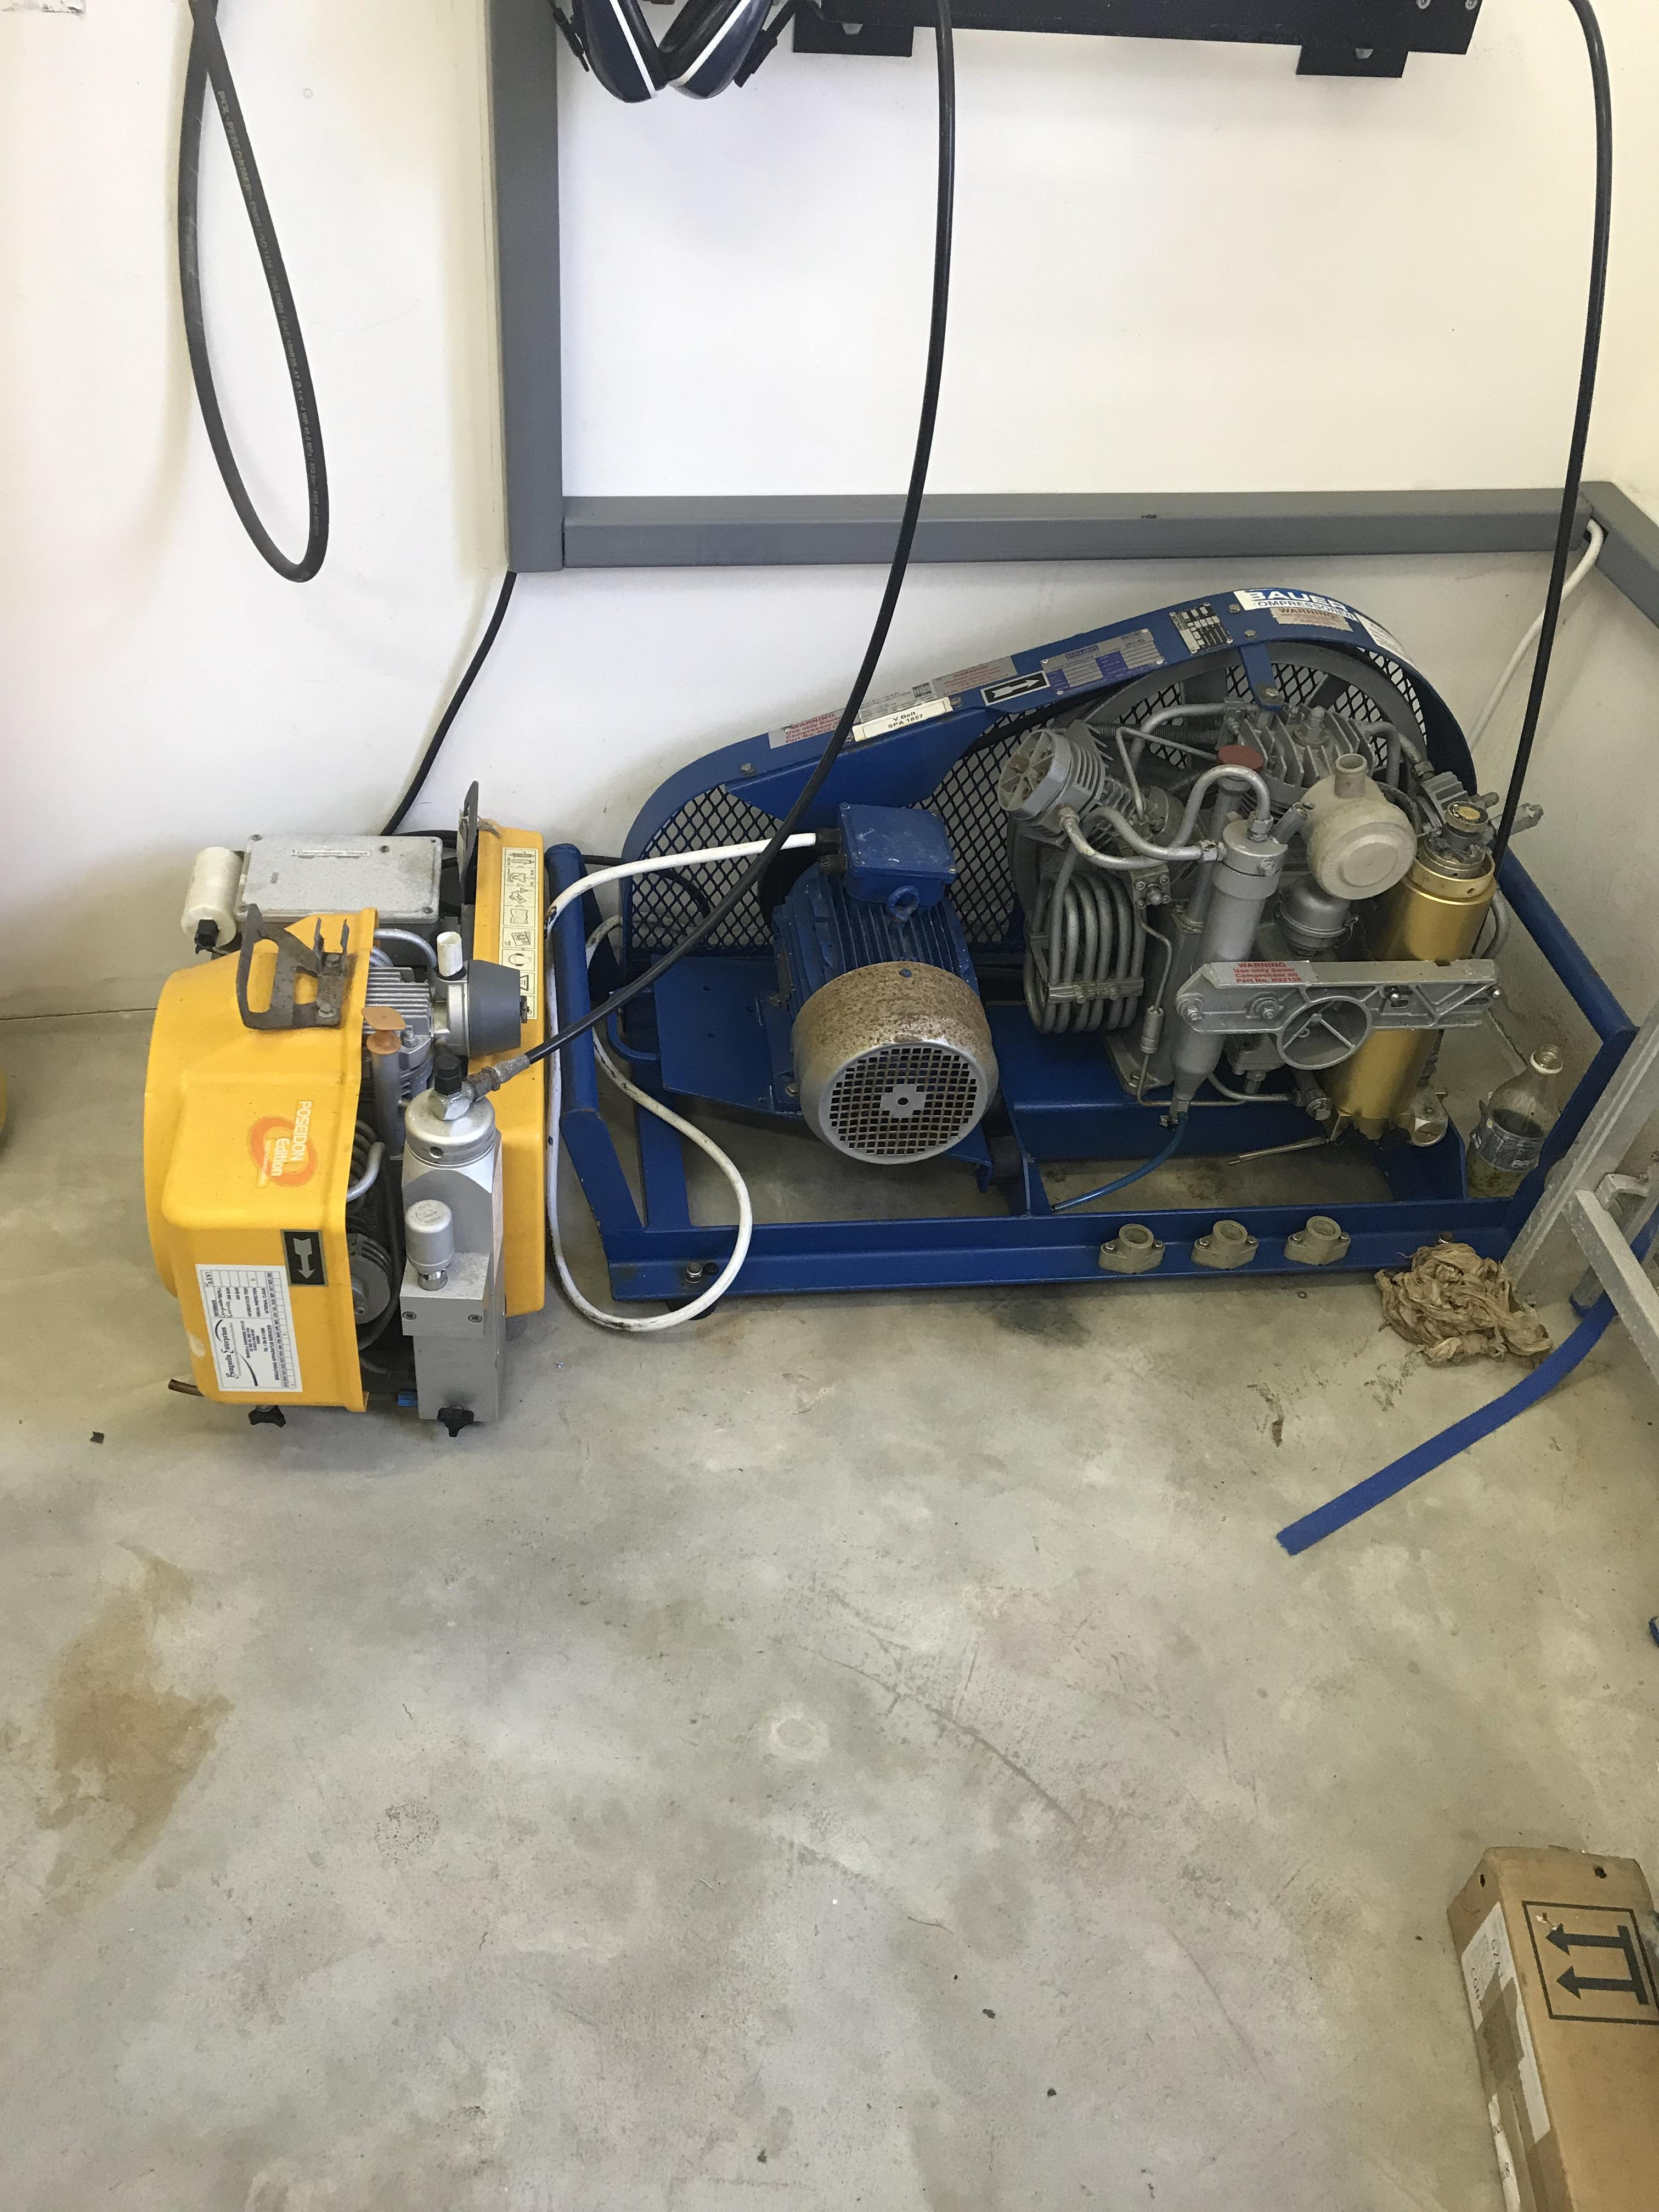
\includegraphics[width=0.5\textwidth,height=\textheight]{images/dive_cylinders/compressors2.jpg}

}

\caption{\label{fig-compressors}Image of the small Poseidon (yellow) and
large Bauer (blue) air compressors used in the Aquarium's Cascading
filling system.}

\end{figure}

In this system, air decants into dive cylinders from an air bank
(Figure~\ref{fig-airbank}), while simultaneously being topped up by the
air compressor. The air bank is maintained to ensure the dive cylinders
can still be filled up if the compressor is not working.

\begin{figure}[H]

{\centering 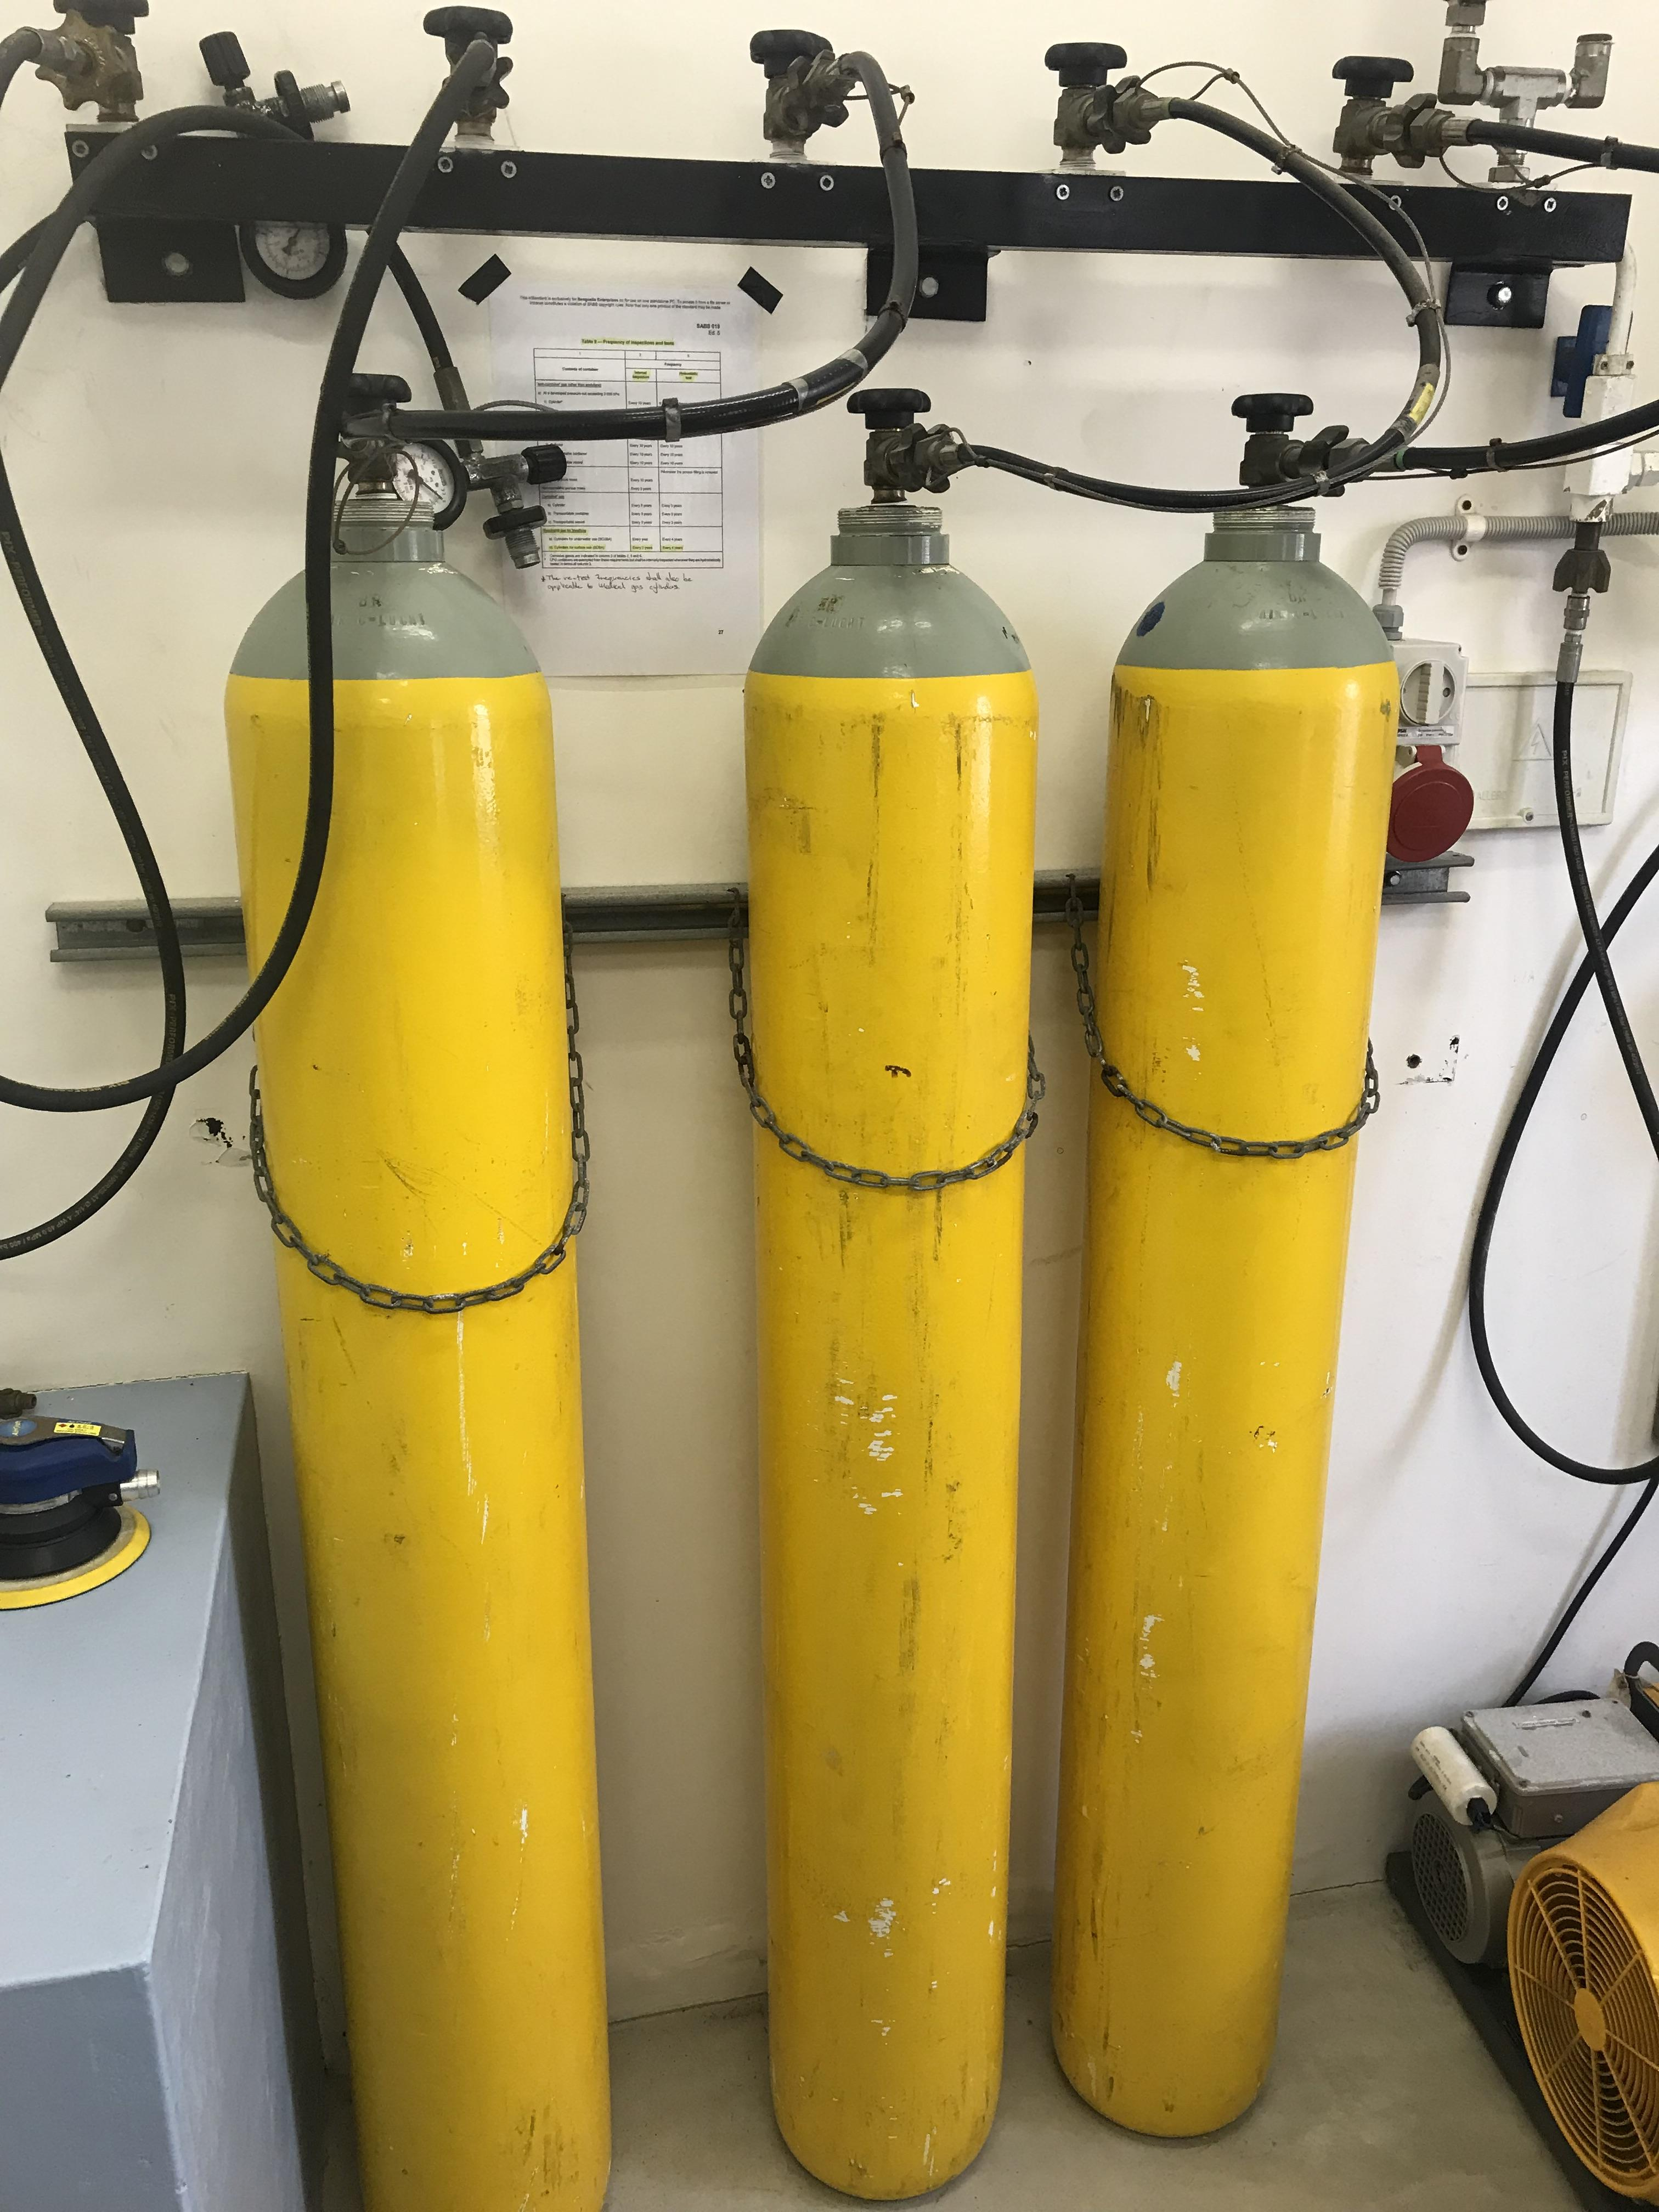
\includegraphics[width=0.5\textwidth,height=\textheight]{images/dive_cylinders/airbank2.jpg}

}

\caption{\label{fig-airbank}These 50\(l\) gas cylinders constitute the
air bank from which air is decanted into the dive cylinders.}

\end{figure}

There are 10 small (10\(l\)) and 3 larger (50\(l\)) cylinders used for
diving and for the air bank, respectively. The dive cylinders are kept
close to a mounted wall heater to keep their temperatures from dropping
too low and thus, preventing condensation on the tanks outer surface
(Figure~\ref{fig-divecyl}).

\begin{figure}[H]

{\centering 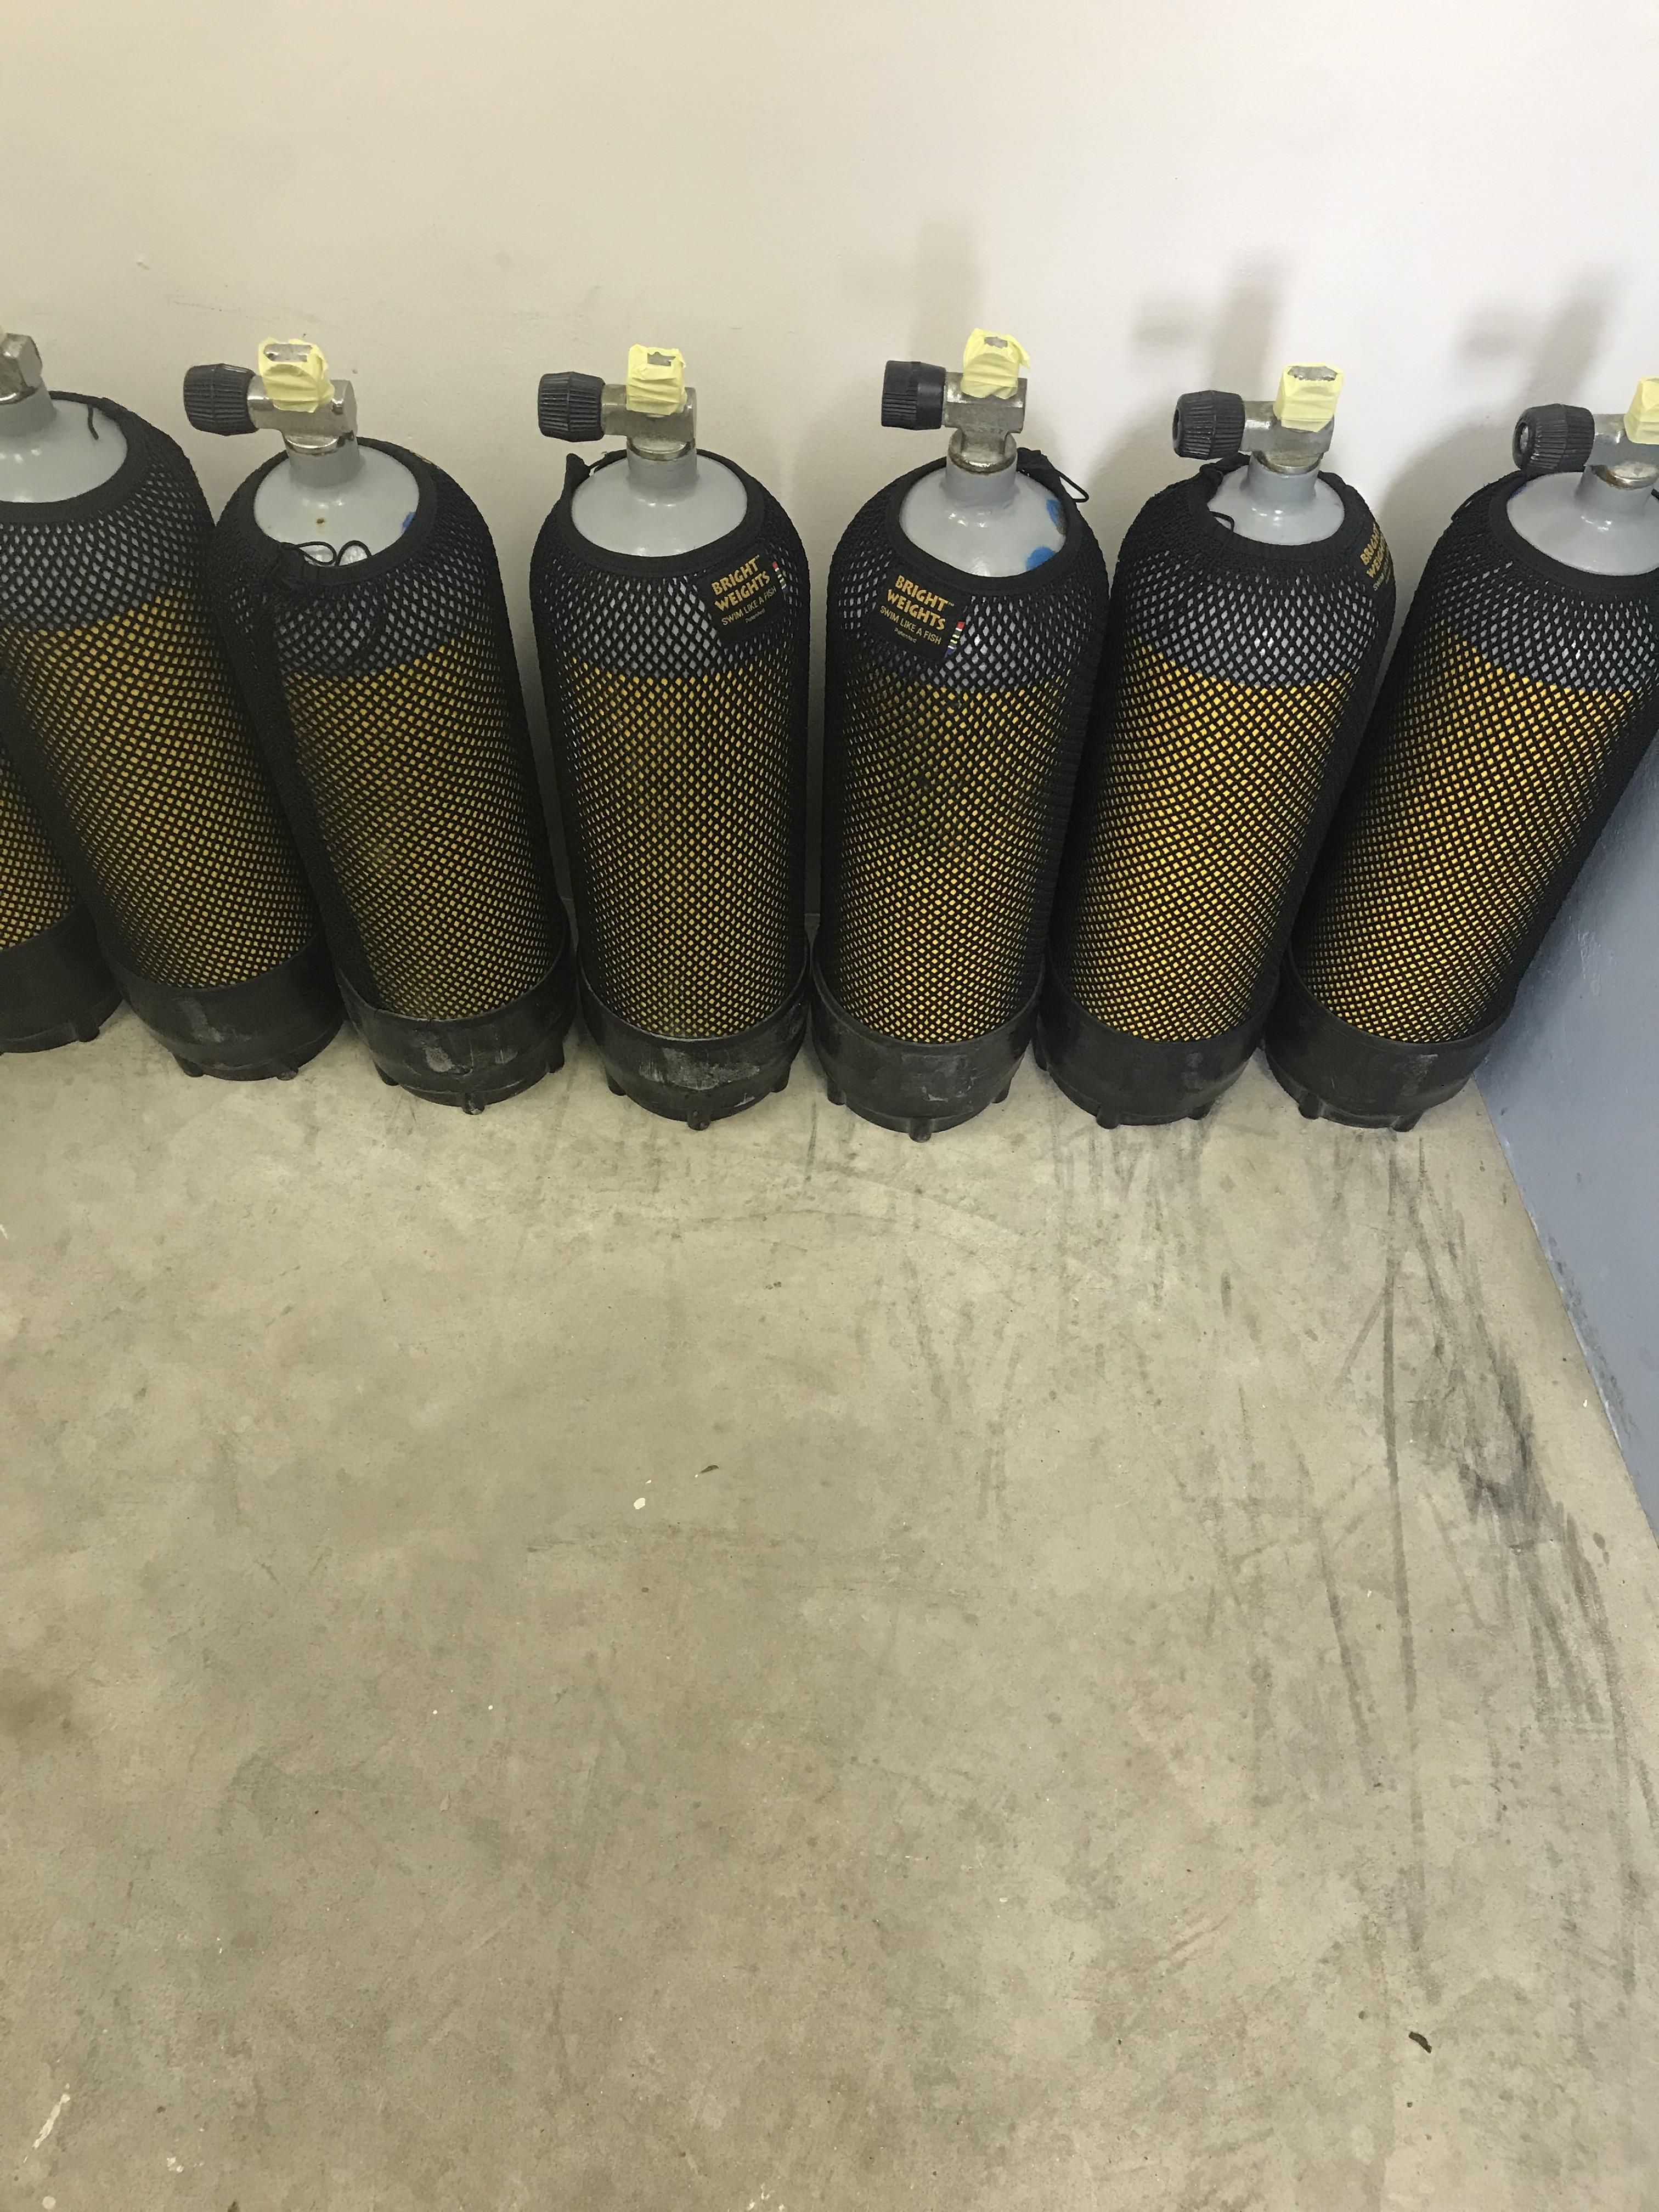
\includegraphics[width=0.5\textwidth,height=\textheight]{images/dive_cylinders/divecyl2.jpg}

}

\caption{\label{fig-divecyl}The 10 10\(l\) cylinders used for diving,
each with their air inlets covered.}

\end{figure}

{Only the Bauer compressor is currently operational}.

\textbf{For the sake of convenience, ensure that the majority of the
dive cylinders are always filled with air i.e., there should never be
more than 2 empty cylinders at a time}.

\begin{enumerate}
\def\labelenumi{\arabic{enumi}.}
\tightlist
\item
  Lift the empty dive cylinders and leave them standing up right.

  \begin{itemize}
  \tightlist
  \item
    \emph{When empty, the dive cylinders are left laying horizontally on
    the ground with their air inlets exposed}.
  \item
    \emph{The tanks should never be completely depleted (leave them at
    approximately 20bar before refill)}.
  \end{itemize}
\item
  Examine the Bauer compressor's oil level.

  \begin{itemize}
  \tightlist
  \item
    \emph{Use the dipstick found at the top of the compressor}
    (Figure~\ref{fig-compressors}).
  \item
    \emph{If the compressor's oil level is low, refill with spare Bauer
    compressor oil found in the cupboard next to the compressor in the
    Workshop}.
  \end{itemize}
\end{enumerate}

\begin{itemize}
\tightlist
\item
  \textbf{If there is no oil in stock, more can be obtained from
  Benguela enterprises (Contact Mr.~Roberto)}.
\end{itemize}

\begin{enumerate}
\def\labelenumi{\arabic{enumi}.}
\setcounter{enumi}{2}
\tightlist
\item
  Connect the filler whips (Figure~\ref{fig-bankrack}), from the air
  bank, to the air inlet of the empty cylinders.

  \begin{itemize}
  \tightlist
  \item
    \emph{The valves on the air bank valve rack and 50}\(l\) air
    cylinders should be left open when not in use
    (Figure~\ref{fig-bankrack}).
  \item
    \emph{Secure the whips to the cylinders by tightening the threaded
    coupling of the lock valves}.
  \end{itemize}
\end{enumerate}

\begin{figure}[H]

\begin{minipage}[t]{0.33\linewidth}

{\centering 

\raisebox{-\height}{

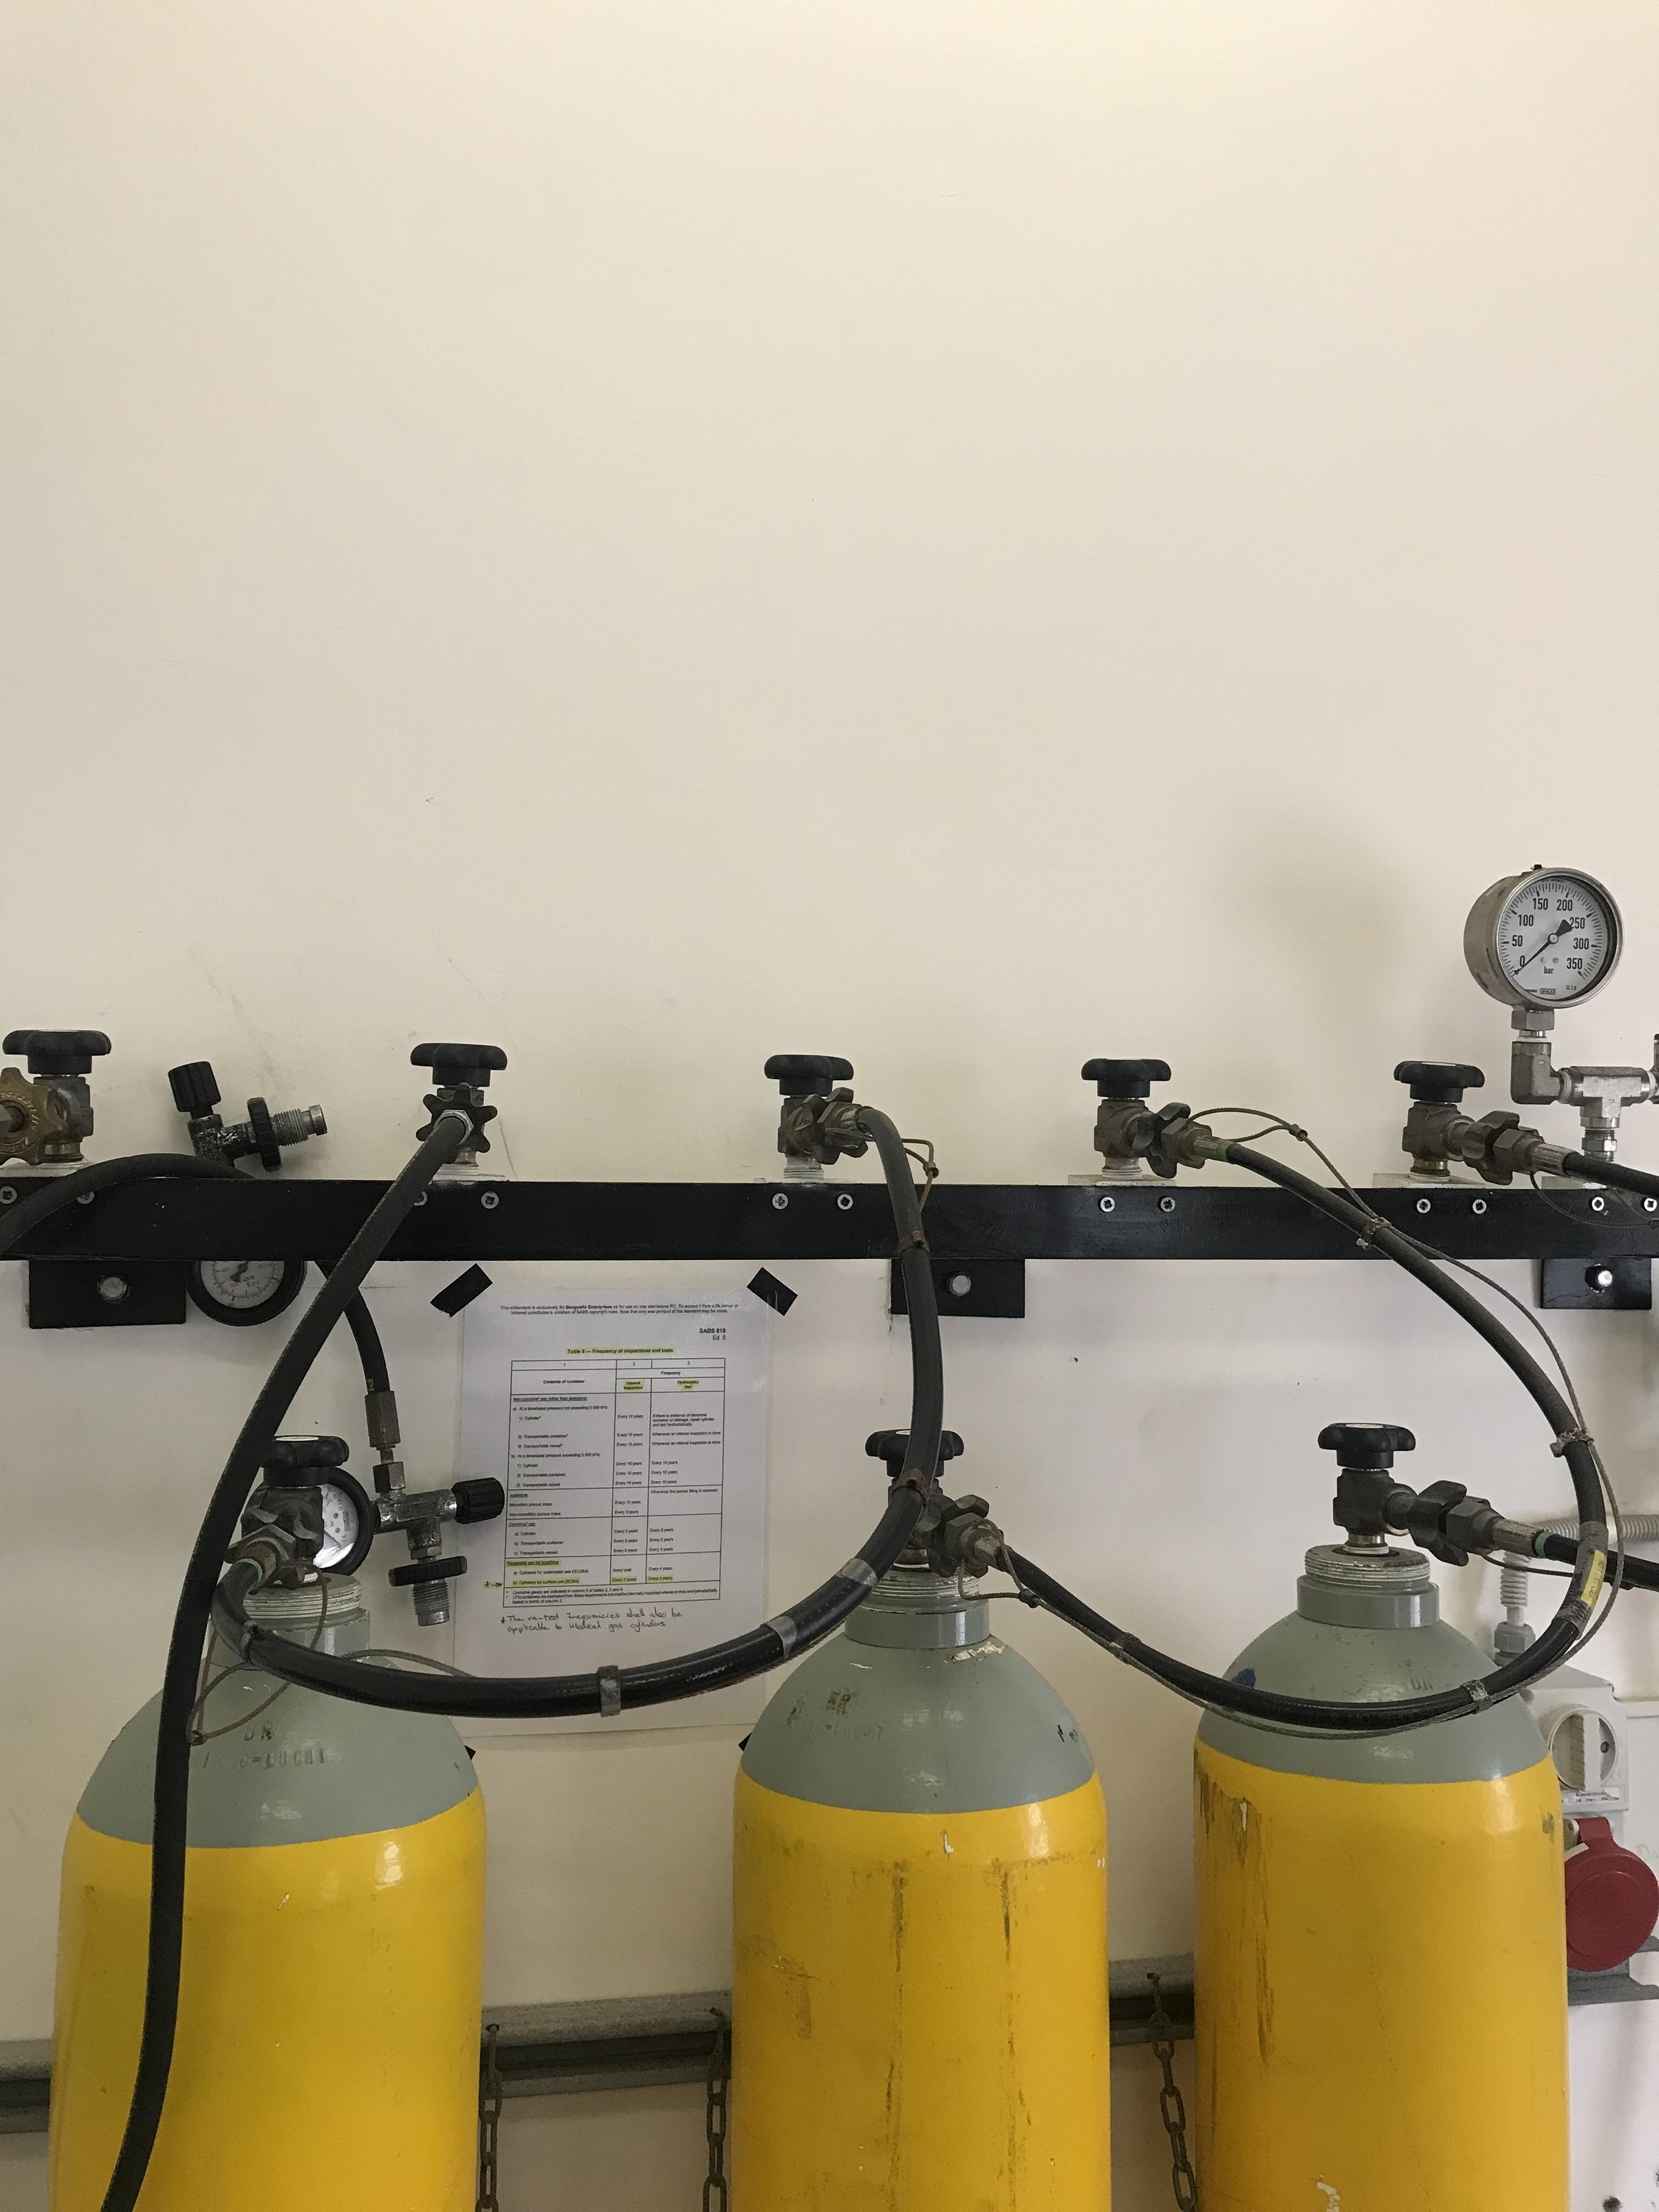
\includegraphics{images/dive_cylinders/bank_rack2.jpg}

}

}

\subcaption{\label{fig-frac-drain}Valve rack}
\end{minipage}%
%
\begin{minipage}[t]{0.33\linewidth}

{\centering 

\raisebox{-\height}{

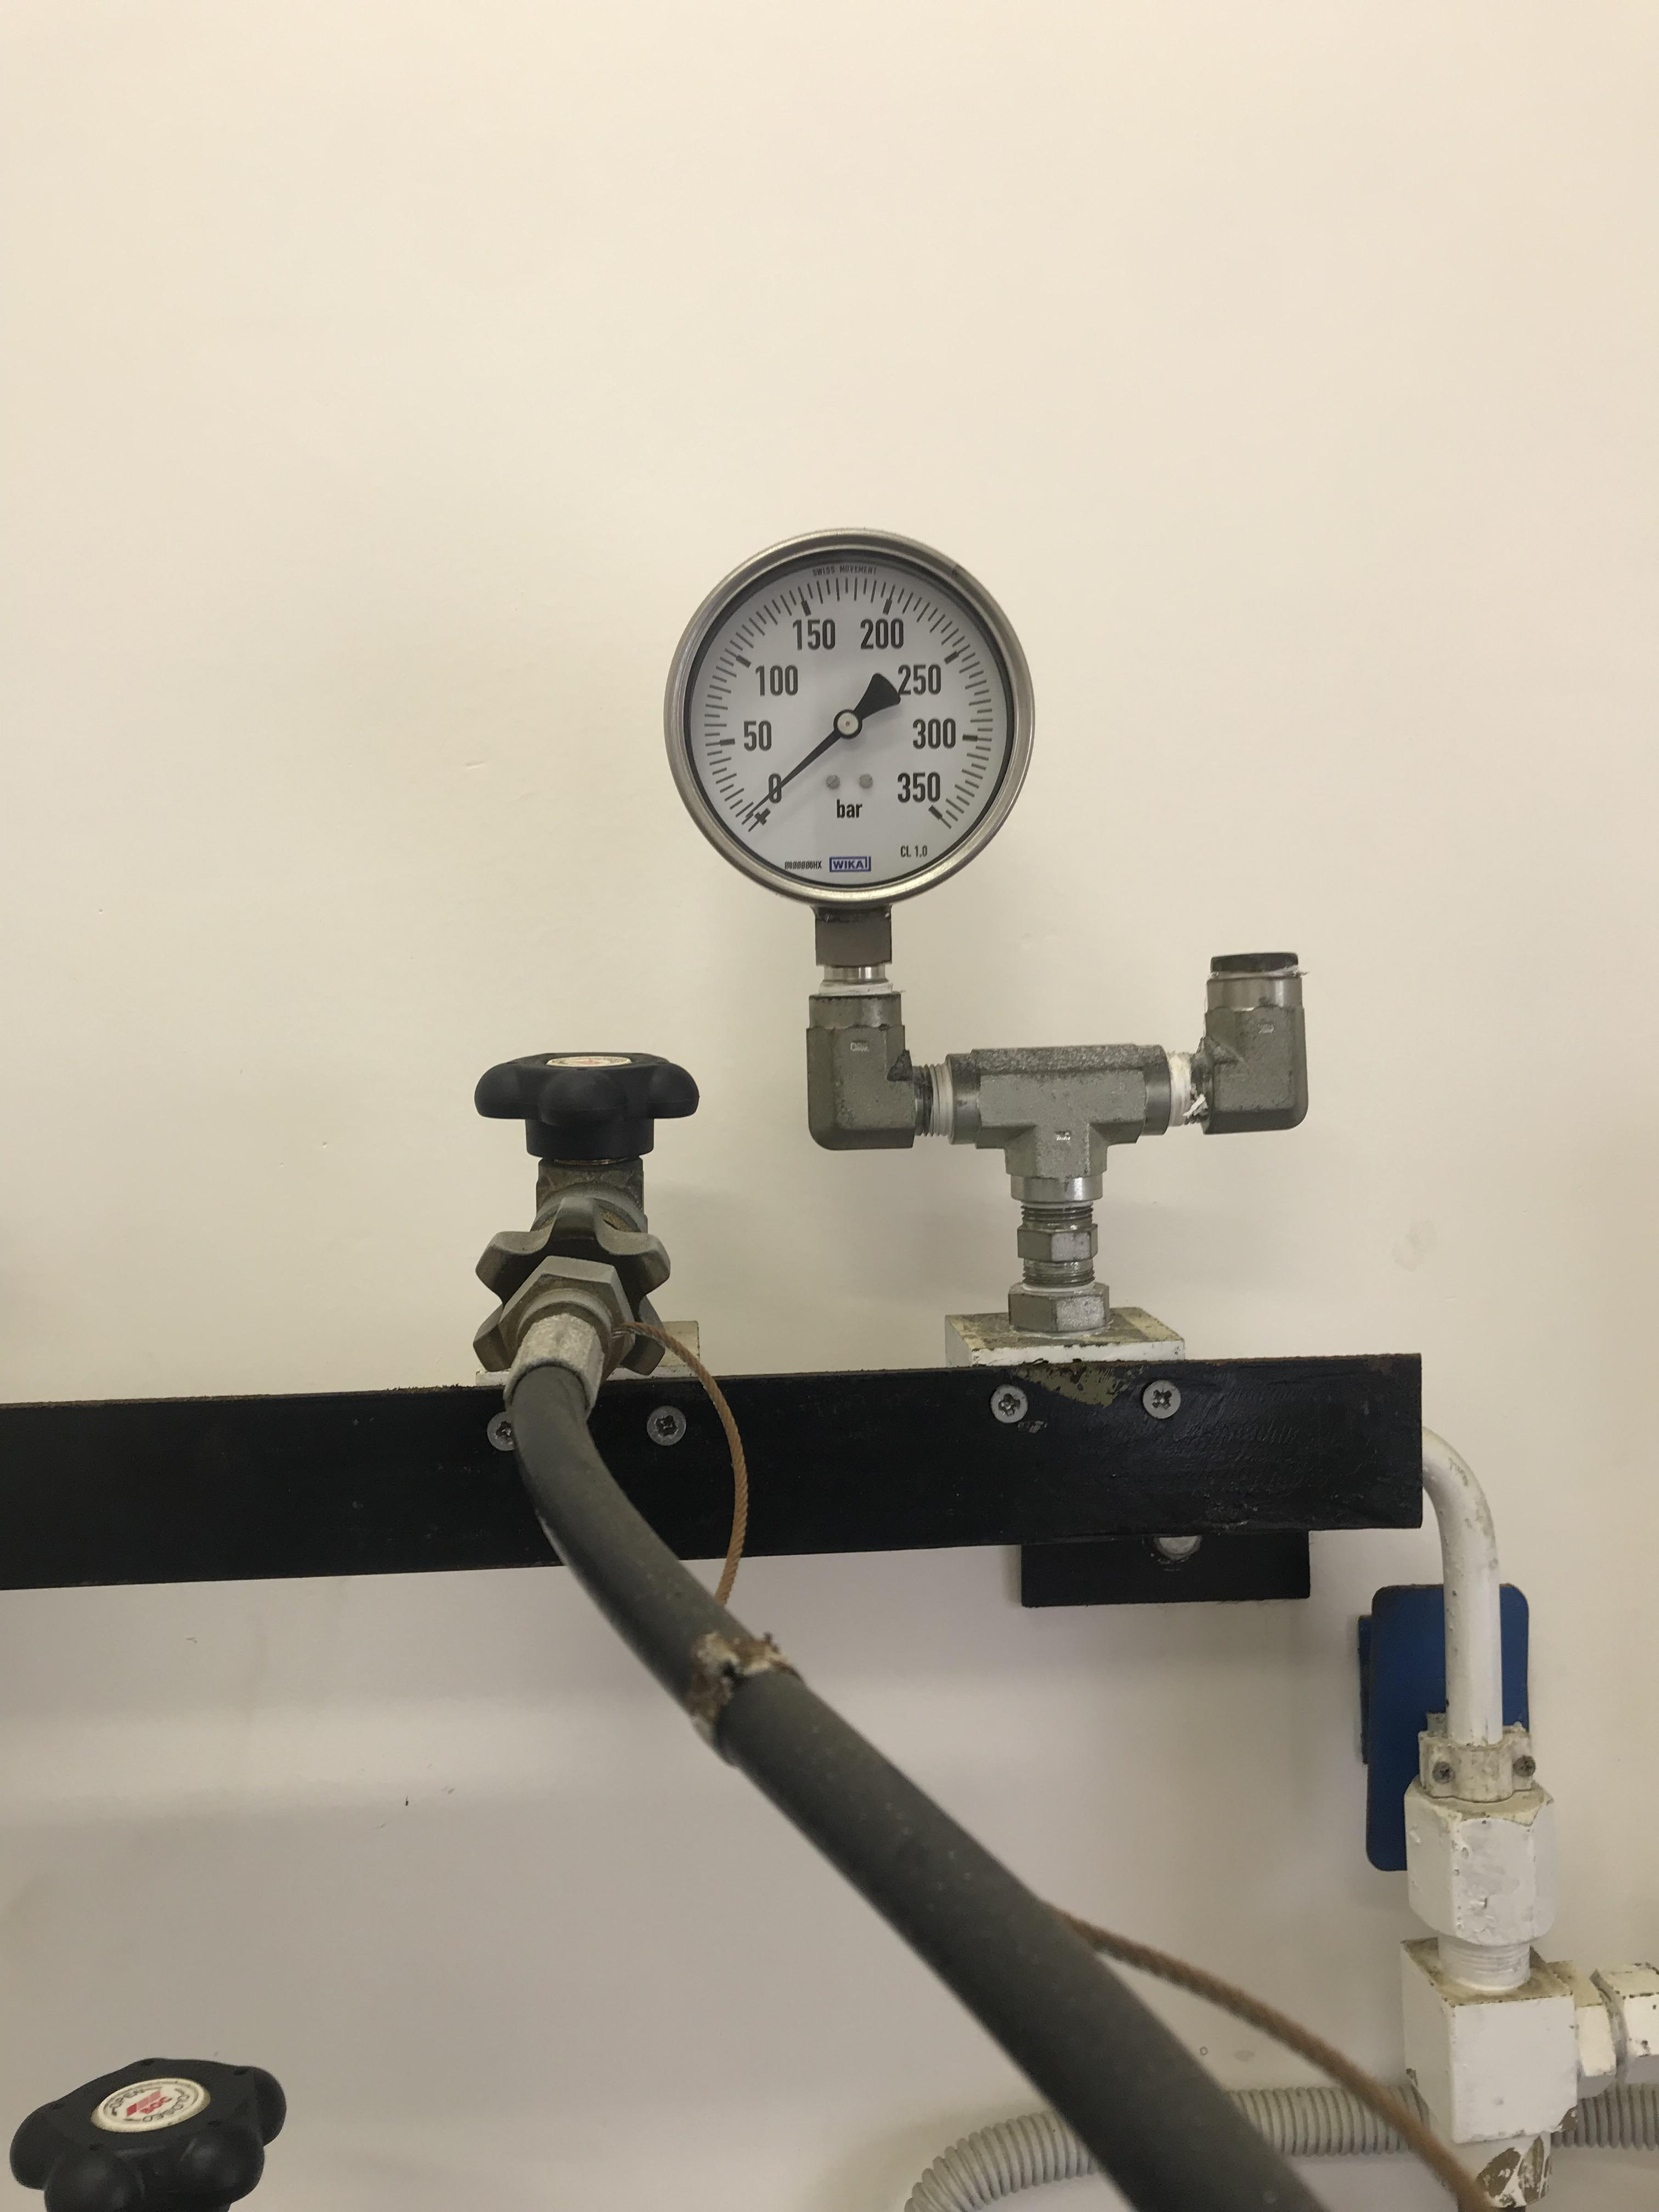
\includegraphics{images/dive_cylinders/bank_mano2.jpg}

}

}

\subcaption{\label{fig-frac-outlet}Manometer}
\end{minipage}%
%
\begin{minipage}[t]{0.33\linewidth}

{\centering 

\raisebox{-\height}{

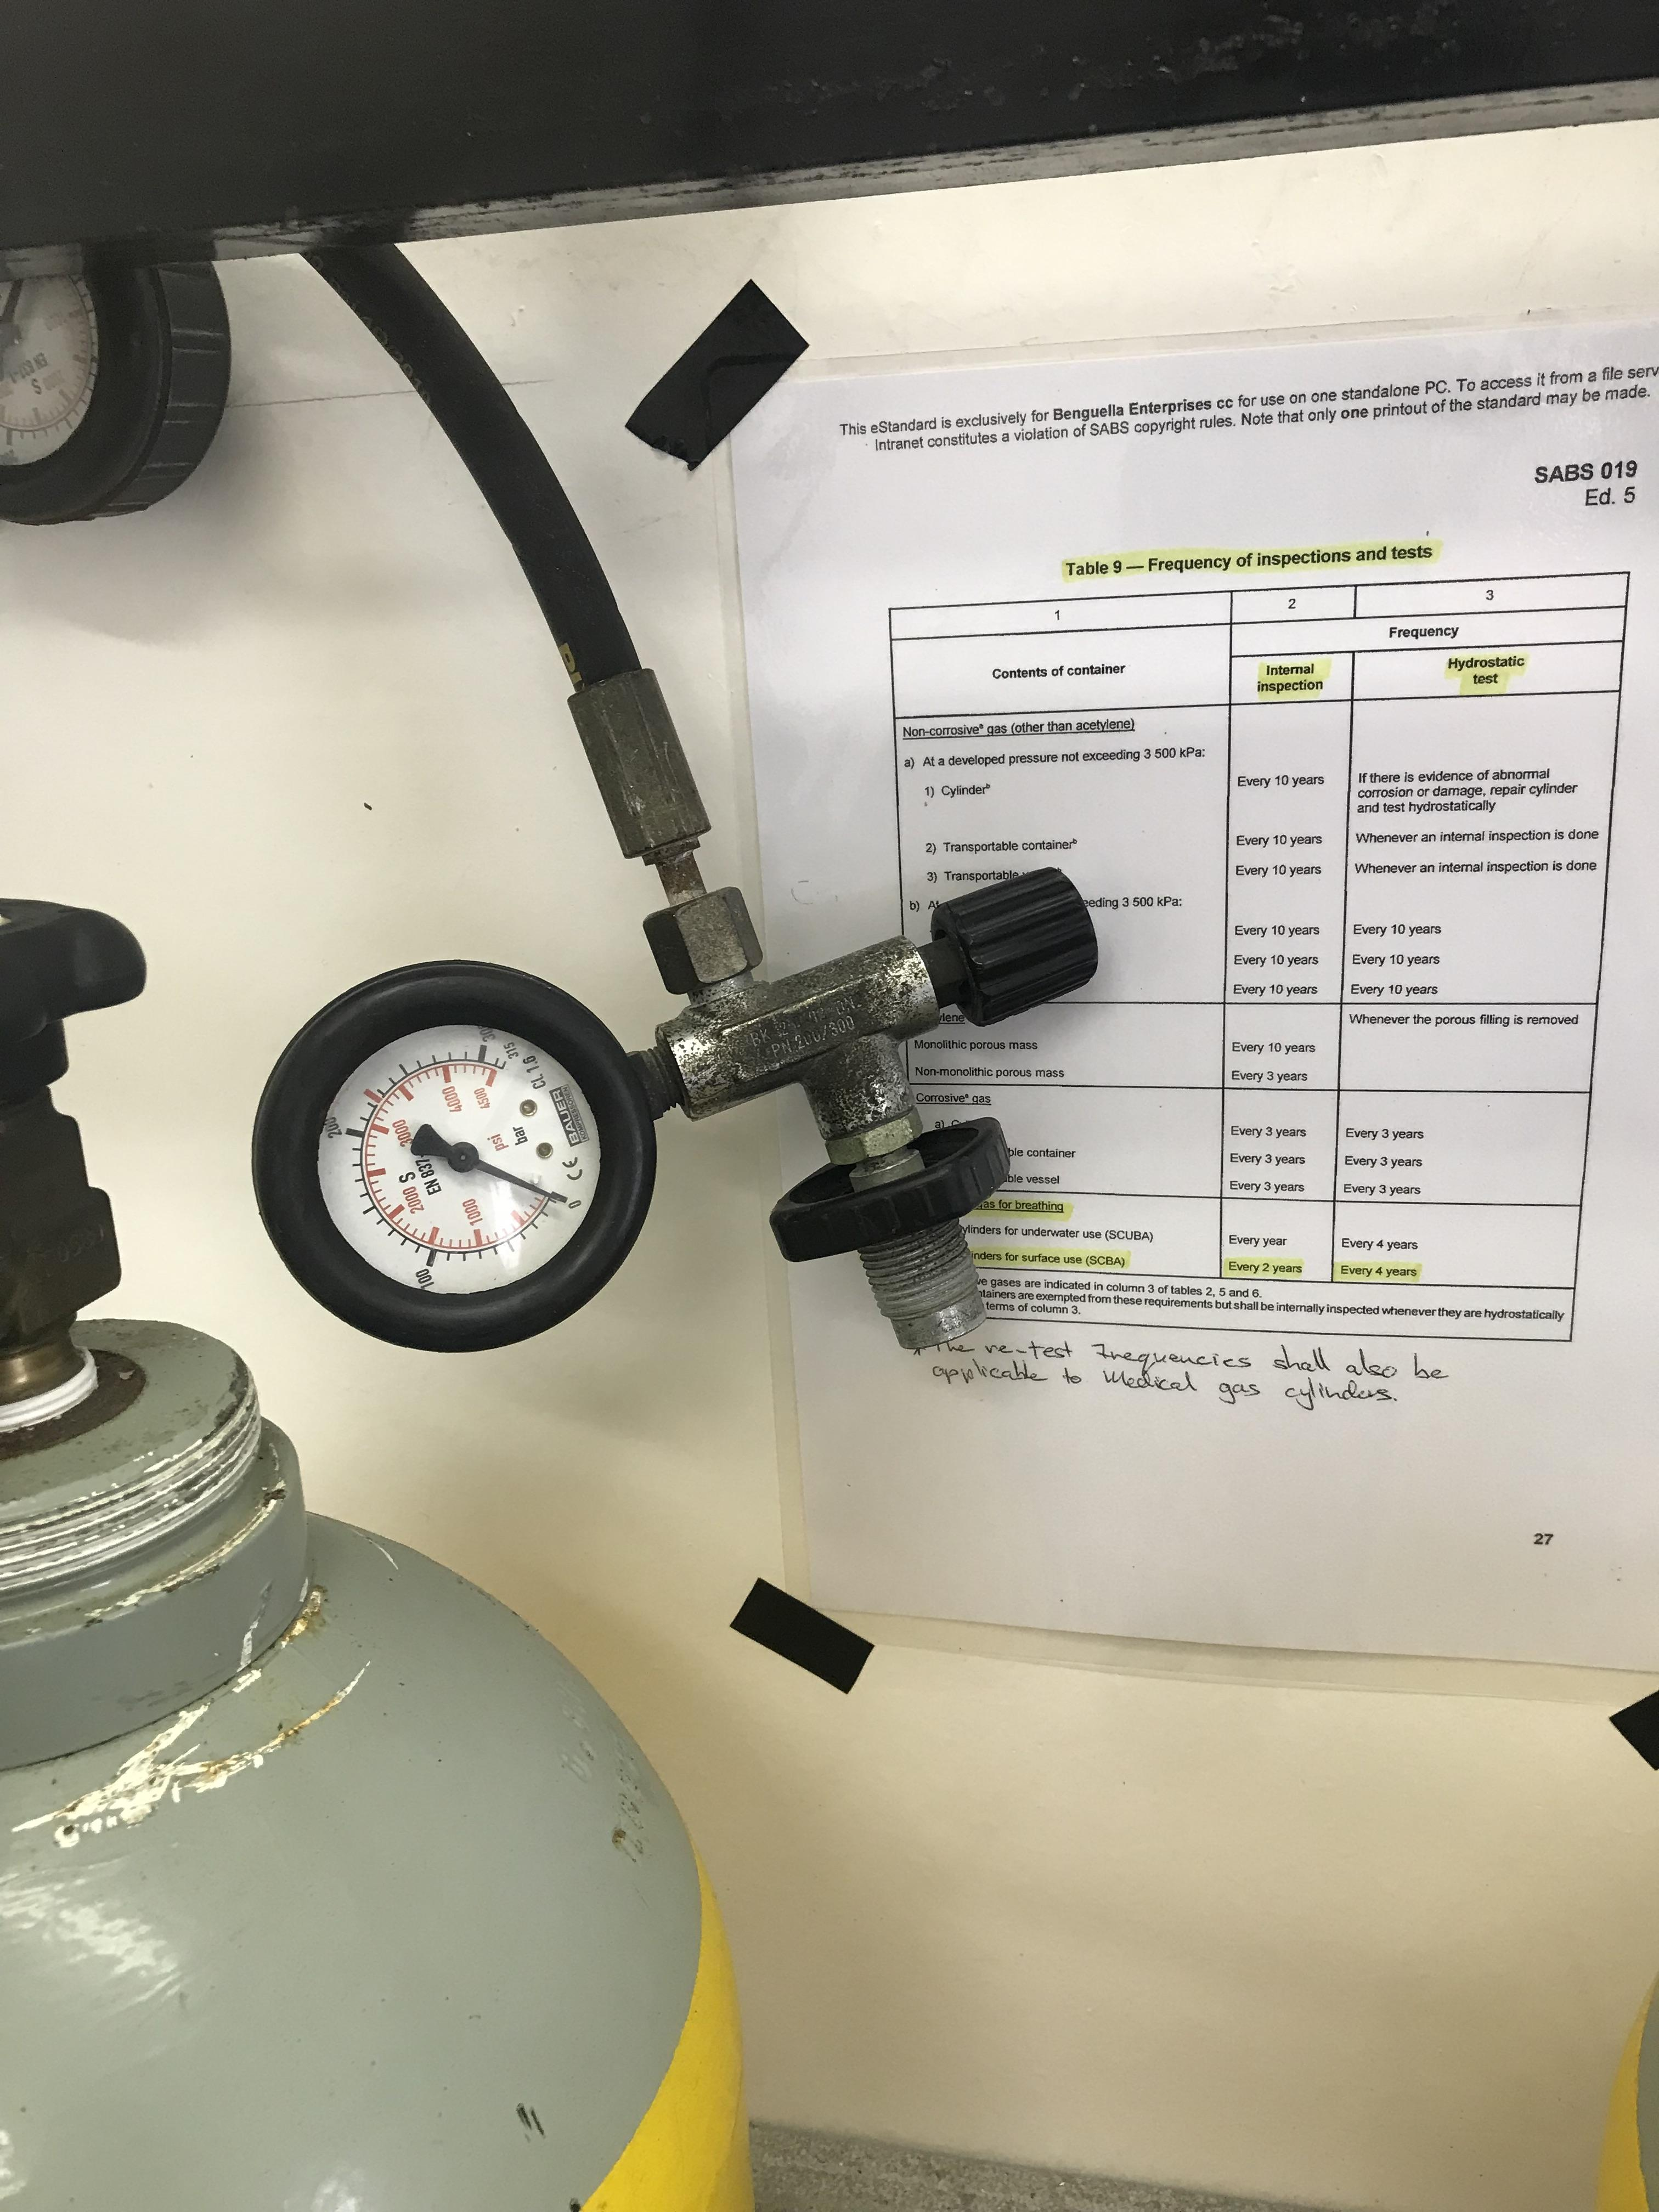
\includegraphics{images/dive_cylinders/fill_whip2.jpg}

}

}

\subcaption{\label{fig-frac-inlet}Filler whip}
\end{minipage}%

\caption{\label{fig-bankrack}Image of the air bank's valve rack and
corresponding parts.}

\end{figure}

\begin{enumerate}
\def\labelenumi{\arabic{enumi}.}
\setcounter{enumi}{3}
\tightlist
\item
  Close the pressure release valves on the connected filler whip
  (Figure~\ref{fig-bankrack}).

  \begin{itemize}
  \tightlist
  \item
    \emph{Turn clockwise}.
  \end{itemize}
\item
  Open the air discharge valve on the filler whips.
\item
  Open the air inlet valves on the empty cylinders.

  \begin{itemize}
  \tightlist
  \item
    \emph{Turn anti-clockwise}.
  \end{itemize}
\end{enumerate}

\begin{figure}[H]

{\centering 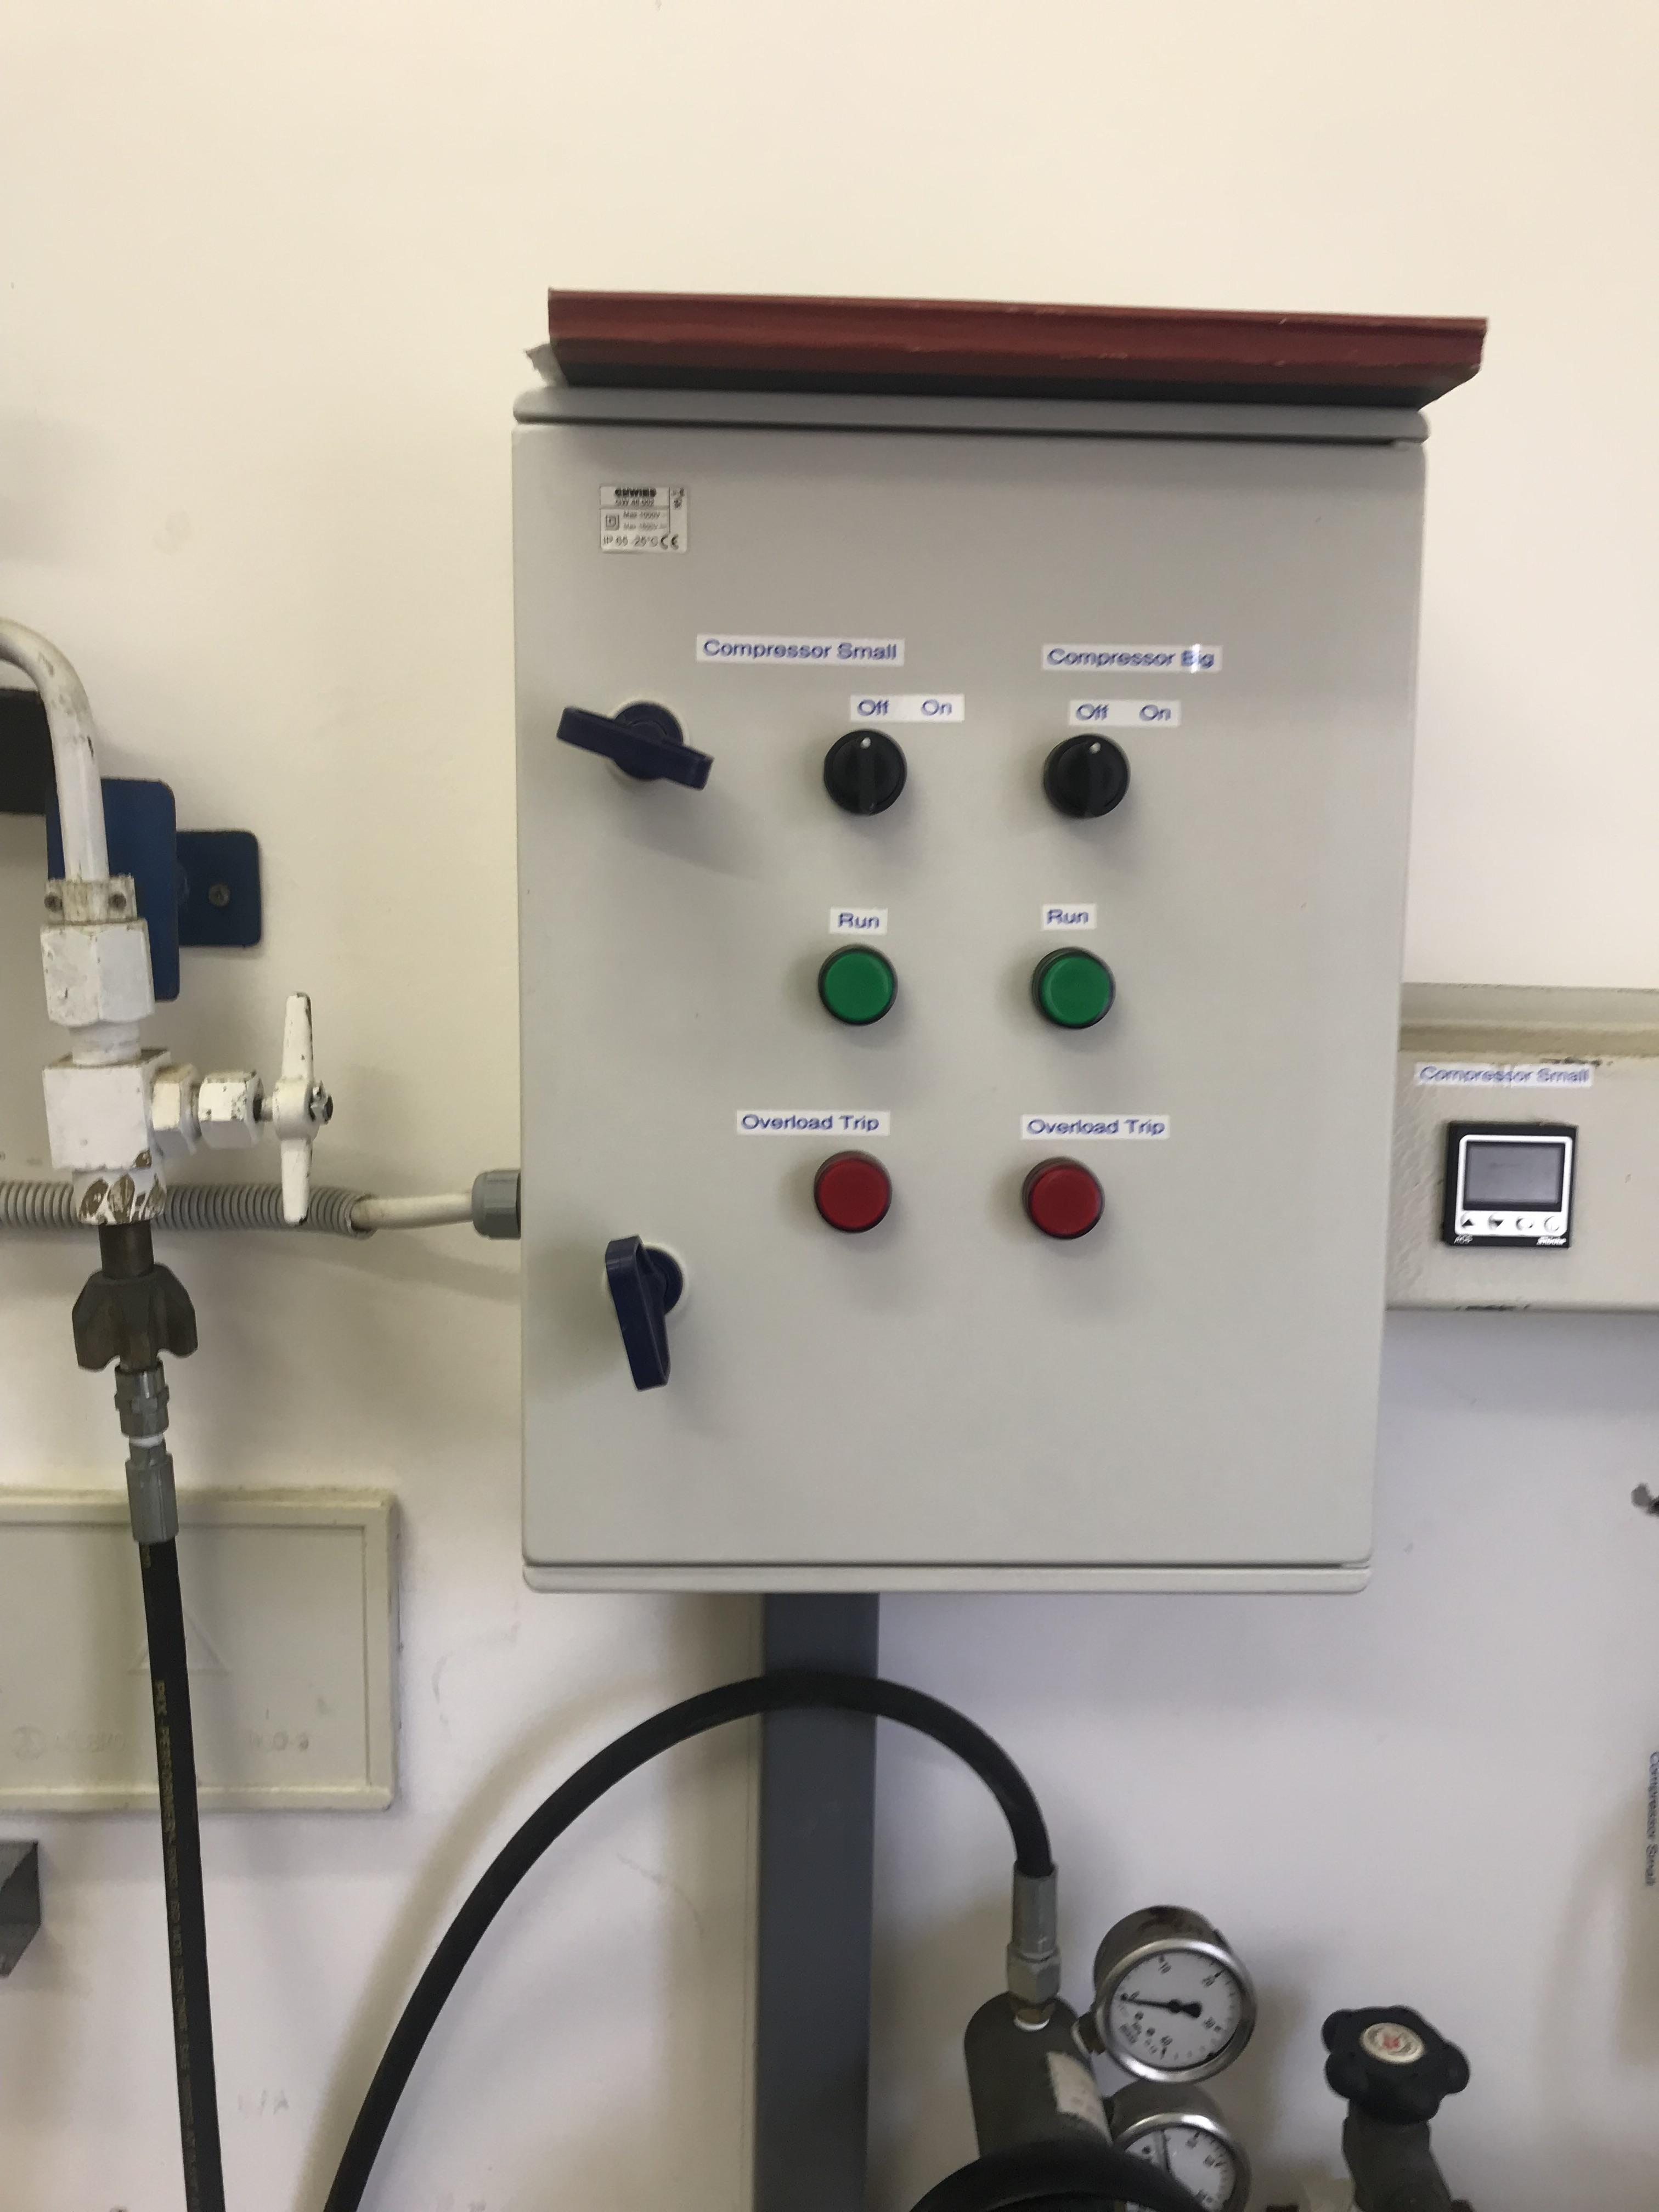
\includegraphics[width=0.5\textwidth,height=\textheight]{images/dive_cylinders/compswitch2.jpg}

}

\caption{\label{fig-compswitch}The compressors' control switchboard with
the compressor log book on top.}

\end{figure}

\begin{enumerate}
\def\labelenumi{\arabic{enumi}.}
\setcounter{enumi}{6}
\tightlist
\item
  Switch the Bauer air compressor (Figure~\ref{fig-compressors}) on and
  press the ``run'' button on the compressor switch board
  (Figure~\ref{fig-compswitch}).
\item
  Allow the cylinders to fill up.

  \begin{itemize}
  \tightlist
  \item
    \emph{The compressor will stop filling the cylinders up
    automatically once they reach 220bar}.
  \item
    \emph{Final pressure can be read from the manometer directly above
    the bank valve rack} (Figure~\ref{fig-bankrack}).
  \item
    \emph{For two cylinders, this will last approximately 25mins}.
  \end{itemize}
\item
  Once full, open the pressure release valve on the filler whip.
\item
  Detach the dive cylinders from their respective filler whips.
\item
  Close the air inlet valves of the dive cylinders.
\item
  Close the air inlet valves of the filler whips.
\item
  Cover the inlet valves of the cylinders' with masking tape and leave
  them standing upright close to the mounted heater next to the other
  cylinders (Figure~\ref{fig-divecyl}).

  \begin{itemize}
  \tightlist
  \item
    \emph{This is done to show that they have recently been filled}.
  \end{itemize}
\item
  Re-rack the filler whips.
\end{enumerate}

\begin{itemize}
\tightlist
\item
  \textbf{For steps 13 and 14, drain the waste fluids into a small used
  bottle} (Figure~\ref{fig-releasevalves}).
\end{itemize}

\begin{enumerate}
\def\labelenumi{\arabic{enumi}.}
\setcounter{enumi}{14}
\tightlist
\item
  Drain the used oil from the compressor.

  \begin{itemize}
  \tightlist
  \item
    \emph{Open the valve on it's bottom left side}
    (Figure~\ref{fig-releasevalves}).
  \end{itemize}
\item
  Decompress the compressor air.

  \begin{itemize}
  \tightlist
  \item
    \emph{Open the two decompression valves on it's bottom right side
    slowly} (Figure~\ref{fig-releasevalves}).
  \end{itemize}
\item
  Close the decompression valves when done.
\end{enumerate}

\begin{figure}[H]

{\centering 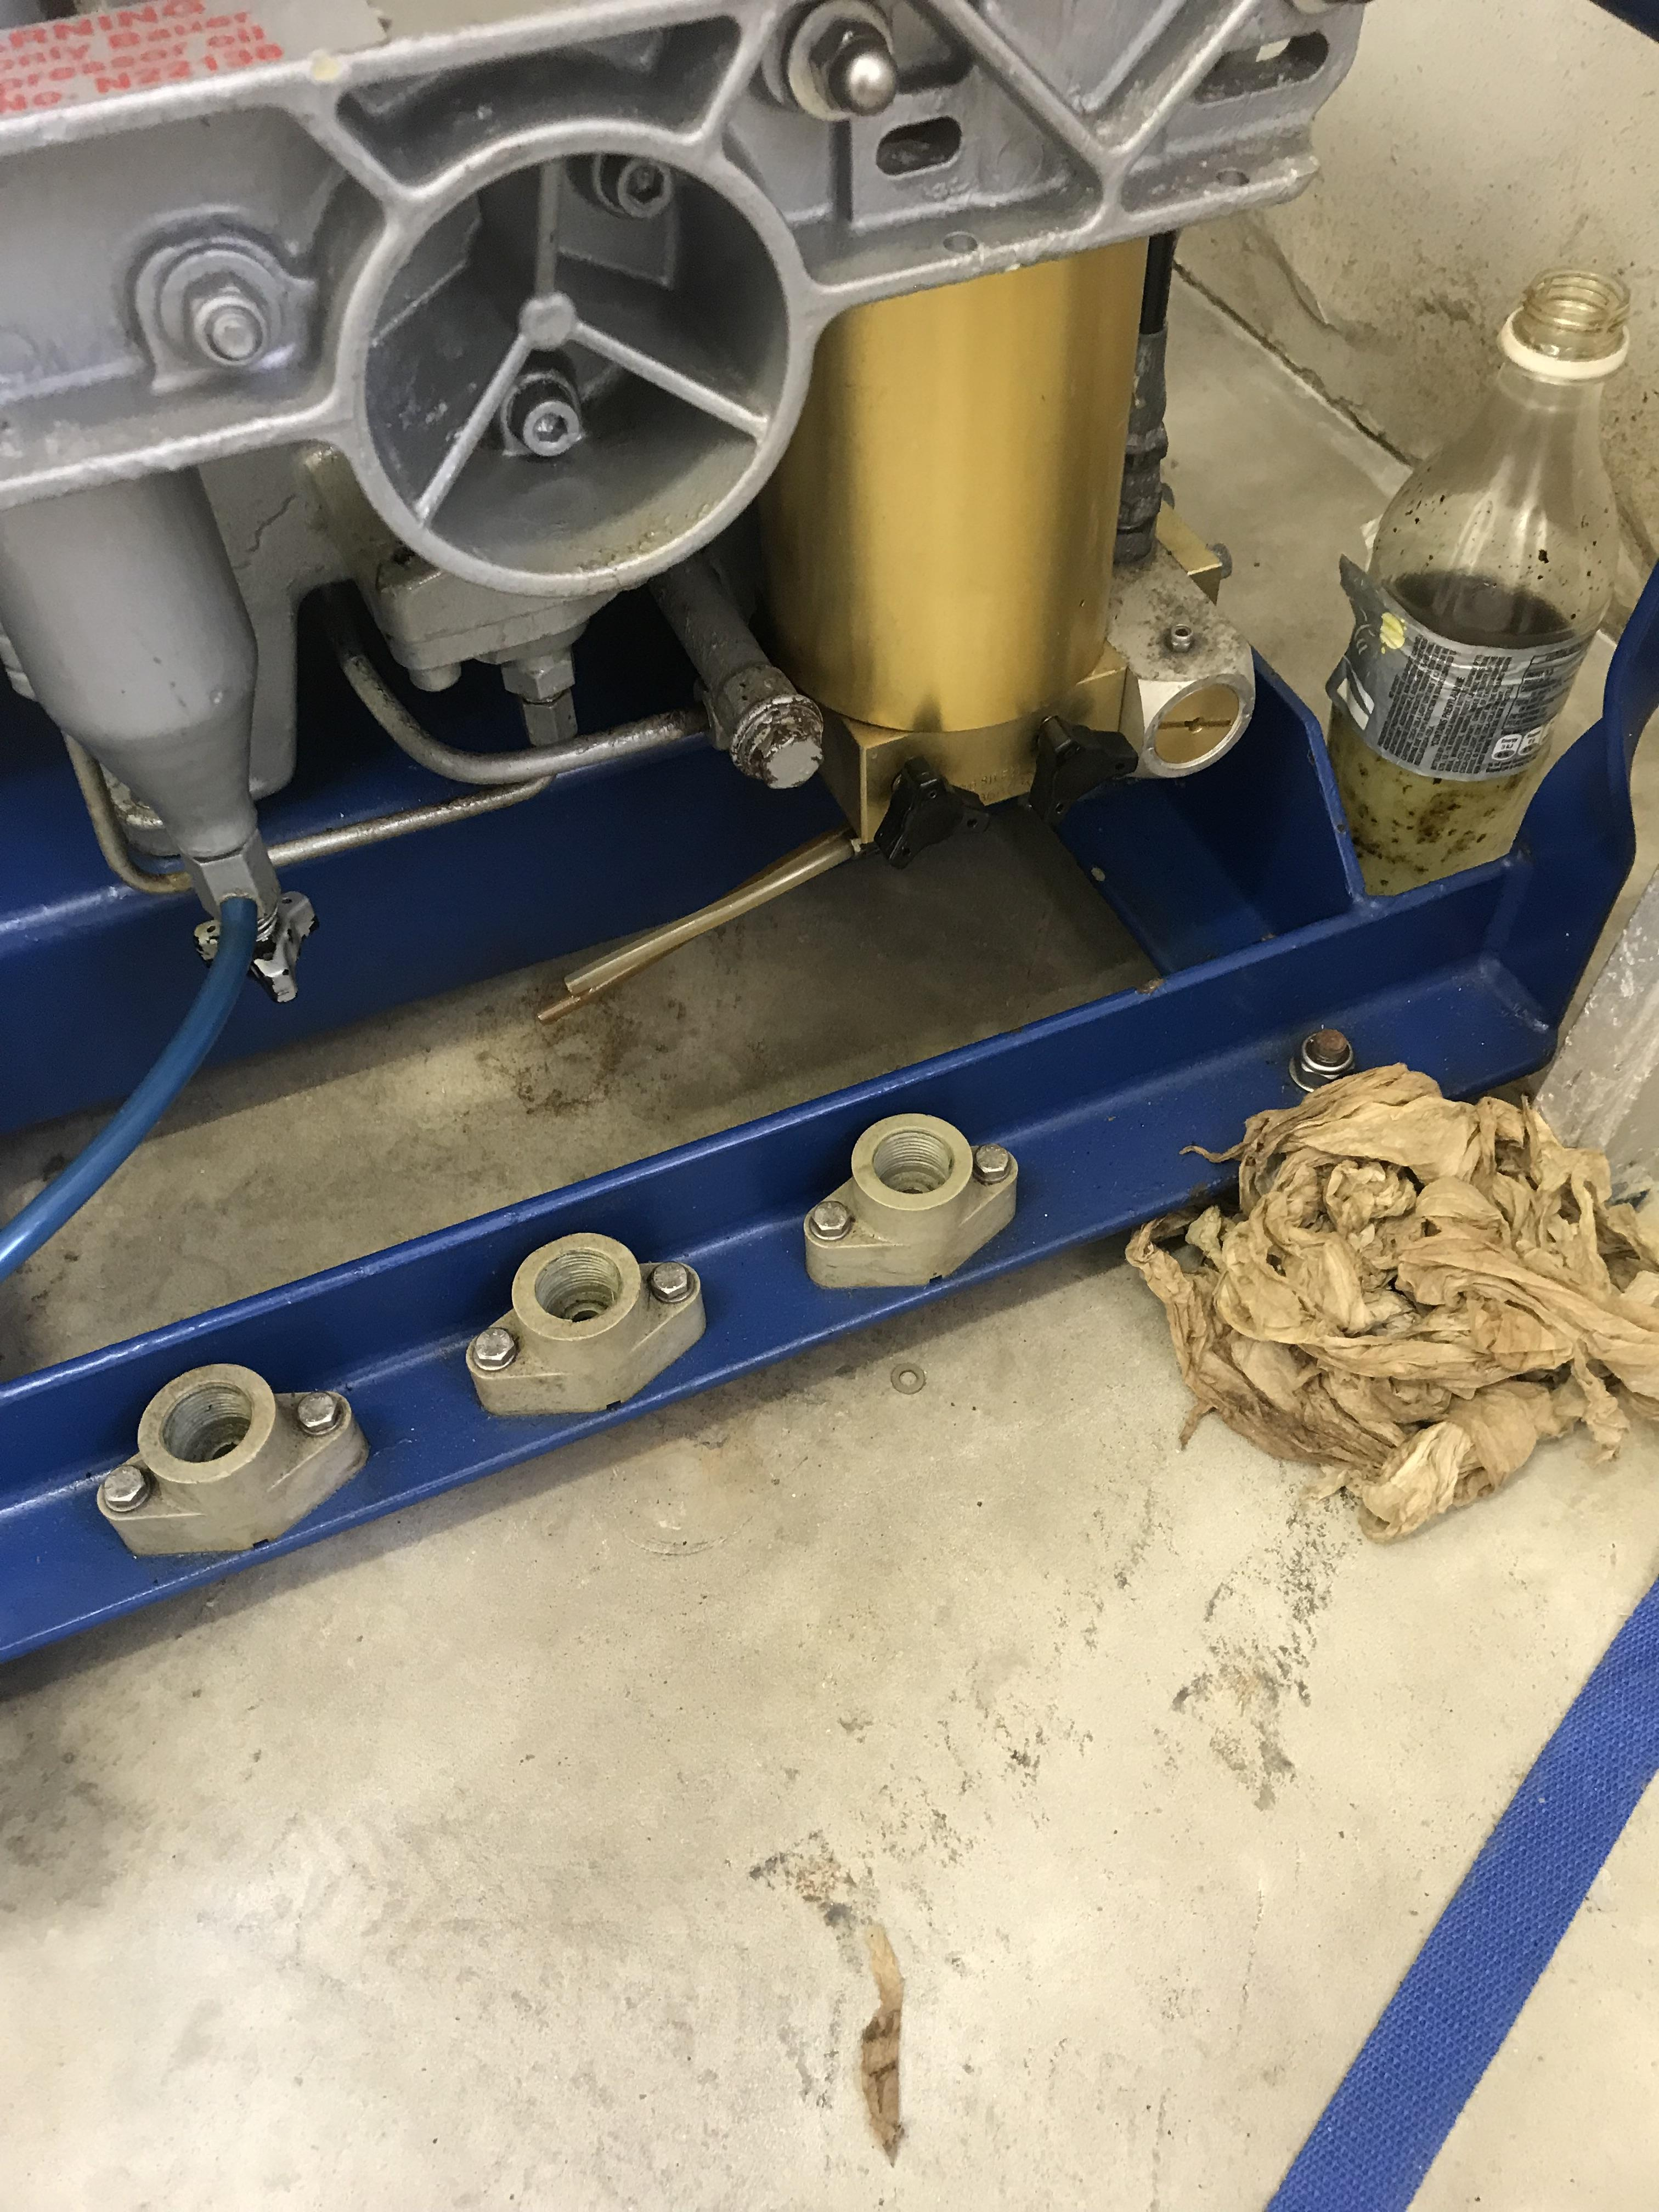
\includegraphics[width=0.5\textwidth,height=\textheight]{images/dive_cylinders/releasevalves2.jpg}

}

\caption{\label{fig-releasevalves}The oil release valves (left, metallic
valve) and decompression valves (right, black valves) found at the
bottom of the Bauer air compressor, along with an old bottle to collect
waste fluid.}

\end{figure}

\begin{enumerate}
\def\labelenumi{\arabic{enumi}.}
\setcounter{enumi}{17}
\tightlist
\item
  Complete the relevant log sheet and book.

  \begin{itemize}
  \tightlist
  \item
    \emph{Found on top of the compressor switch board}
    (Figure~\ref{fig-compswitch}).
  \end{itemize}
\end{enumerate}

\textbf{It is important to let the dive cylinders cool down for at least
6 hours before using them}.

\textbf{The rate at which the air cylinders have to be filled
(cylinders/month), depends almost entirely on how frequently they are
used}.

\hypertarget{disclaimer}{%
\section*{\texorpdfstring{{DISCLAIMER}}{DISCLAIMER}}\label{disclaimer}}
\addcontentsline{toc}{section}{{DISCLAIMER}}

{This section does not claim to provide sufficient details describing
how to operate the Bauer and the Poseidon air compressors. It serves
only as a brief guide to help technicians employed by the MFMR, use the
compressors to fill dive cylinders that will only be used inside the
Aquarium or by Aquarium staff. For a more comprehensive description of
the Aquarium air compressors' operation, please refer to the
``Compressor manual'' provided by the Namibian Underwater Federation. To
ensure that the compressors and dive cylinders are suitably maintained,
it is strongly advised that potential air compressor operators obtain
the appropriate training and/or operator certificates before using them.
It should be understood that the author(s) of this manual do not assume
any laibility for any damage to property/personal injury sustained while
following the instructions in this document.}

\hypertarget{maintenance-1}{%
\section{Maintenance}\label{maintenance-1}}

\hypertarget{repairs-4}{%
\section{Repairs}\label{repairs-4}}

\hypertarget{testing}{%
\section{Testing}\label{testing}}

\newpage

\hypertarget{sec-sample-collection}{%
\chapter{Sample collection}\label{sec-sample-collection}}

The Aquarium only displays live marine animals found along the Namibian
coast. They have to be collected to keep the Aquarium's display tanks
stocked, particularly when replacing dead or sick individuals. This is
generally done by the Technical assistants but, animal collection trips
may also include the Aquarium's technicians. Animal collection is
achieved via several methods, including, Aquarium staff sampling efforts
along nearby rocky and sandy shores; liaising with frequent sport
anglers willing to donate some of their catch; obtaining specific
animals with the help of open water survey crews dispatched on the
research vessels and by accepting live display animal donations from
recreational divers.

\hypertarget{aquarium-staff}{%
\section{Aquarium staff}\label{aquarium-staff}}

Sample collection by aquarium staff is only done to collect some of the
intertidal species, mainly for the Aquarium's small display tanks,
because these are easily accessible. However, sampling in the intertidal
is normally restricted to spring low tides during normal work hours.
Overtime arrangements have to be made if sampling needs to be done
outside of work hours.

{This can be completed by two members of staff.}

\hypertarget{sec-collect-tool}{%
\subsection{Tool preparation}\label{sec-collect-tool}}

\textbf{Most of the tools required can be found in the quarantine area
or in the workshop (room 162)}.

These include:

\begin{itemize}
\tightlist
\item
  2 x waders.
\item
  1 x small mosquito fish net.

  \begin{itemize}
  \tightlist
  \item
    \emph{Edges knit together to create a funnel with a closed tapered
    end}.
  \end{itemize}
\item
  buckets.

  \begin{itemize}
  \tightlist
  \item
    \emph{Number of buckets depends on number of animals being
    collected}.
  \item
    \emph{Make sure there are enough}.
  \end{itemize}
\item
  2 x fish scoop nets.
\item
  2 x pair of work gloves.
\item
  2 x small scrapers.
\item
  2 x knives
\end{itemize}

\textbf{The item list above was drafted with only two staff members in
mind}. \textbf{Pack accordingly}.

\hypertarget{sample-sites}{%
\subsection{Sample sites}\label{sample-sites}}

This section lists some of the sample sites frequented by Aquarium staff
during sampling trips and the associated intertidal animals and
respective collection methods.

\textbf{All fish can be caught using the mosquito net}.\textbf{Two
members of technical staff will hold the top and bottom of the net,
keeping it open under water whilst wading to trap any fish in the
funnel}.

\begin{itemize}
\tightlist
\item
  Longbeach tidal pool area.

  \begin{itemize}
  \tightlist
  \item
    \emph{One of the more commonly visited sites}.
  \item
    \emph{Longbeach is a small residential area found between Swakopmund
    and Walvis bay}.
  \item
    \emph{Large tidal pool can be found on the far right (North) end}.
  \item
    Animals found here include:

    \begin{itemize}
    \tightlist
    \item
      Silver side fish (\emph{Chelon richardsonii})

      \begin{itemize}
      \tightlist
      \item
        \emph{Inside the tidal pool}.
      \end{itemize}
    \item
      Dassies/Blacktail (\emph{Diplodus sargus capensis})

      \begin{itemize}
      \tightlist
      \item
        \emph{Inside the tidal pool}.
      \end{itemize}
    \item
      Brittle star fish (\emph{Ophioderma wahlbergi})

      \begin{itemize}
      \tightlist
      \item
        \emph{Found buried under sand in intertidal sandy shores or
        under low shore rocks}.
      \item
        \emph{Collect them by hand}.
      \end{itemize}
    \item
      Klipfish (\emph{Clinus venustris})

      \begin{itemize}
      \tightlist
      \item
        \emph{In the tidal pool}.
      \end{itemize}
    \item
      White mussels (\emph{Donax serra})

      \begin{itemize}
      \tightlist
      \item
        \emph{Found buried in the intertidal sandy beach, normally
        towards the end of the wave swash}.
      \item
        \emph{Located via a process commonly known as the ``Mussel
        jive'' (swivel heel of foot in the sand using a windshield wiper
        motion until you feel the mussel) during receding waves of the
        receding low tide}.
      \item
        \emph{Can then be dug up by hand}.
      \end{itemize}
    \end{itemize}
  \end{itemize}
\item
  Baddewanne rocky shore.

  \begin{itemize}
  \tightlist
  \item
    \emph{Also commonly visited, particularly to collect Ulva to feed
    the Sea hares and limpets for the Rock suckers}.
  \item
    \emph{First stretch of rocky shore between Swakopmund and
    Longbeach}.
  \item
    Animals found here include:

    \begin{itemize}
    \tightlist
    \item
      Granite limpet (\emph{Cymbula granatina})

      \begin{itemize}
      \tightlist
      \item
        \emph{Attached to mid shore rocks}.
      \item
        \emph{Removed from the rocks by carefully and quickly sliding
        the small scraper underneath each limpet's foot}.
      \end{itemize}
    \item
      Redbait (\emph{Pyura stolonifera})

      \begin{itemize}
      \tightlist
      \item
        \emph{Attached to low shore rocks}.
      \item
        \emph{Detach the Redbait pods from their substrate by hand}.
      \end{itemize}
    \item
      Namibian cushion starfish (\emph{Asterina stellifera})

      \begin{itemize}
      \tightlist
      \item
        \emph{Collected from low shore rock crevices and under small
        boulders by hand}.
      \end{itemize}
    \item
      Sea hare (\emph{Aplysia spp})

      \begin{itemize}
      \tightlist
      \item
        \emph{Found in under medium sized boulders in rocky intertidal}.
      \item
        \emph{Can be caught by hand and placed in bucket}.
      \end{itemize}
    \item
      Black sea cucumber (\emph{Holothuria atra})

      \begin{itemize}
      \tightlist
      \item
        \emph{Low shore rock crevices and in rock pools}.
      \item
        \emph{Collected by hand}.
      \end{itemize}
    \item
      Crumb-of-bread sponge (\emph{Hymeniacidon perlevis})

      \begin{itemize}
      \tightlist
      \item
        \emph{Low shore rock crevices and rock overhangs}.
      \item
        \emph{Lift the substrate (small rocks or molluscs) up with the
        animal attached}.
      \end{itemize}
    \end{itemize}
  \end{itemize}
\item
  Luderitz rocky shore.

  \begin{itemize}
  \tightlist
  \item
    \emph{Hardly ever visited}.
  \item
    \emph{Southern coast of Namibia, Swakopmund}.
  \item
    Animals found here:

    \begin{itemize}
    \tightlist
    \item
      Sandy anemones (\emph{Bunodactis reynaudi})

      \begin{itemize}
      \tightlist
      \item
        \emph{In intertidal sandy shores}.
      \item
        \emph{Carefully remove the base from the substrate or lift the
        substrate up with the animal attached}.
      \end{itemize}
    \item
      Cape sea urchin (\emph{Parechinus angulosus})
    \item
      \emph{Flat area of low shore rocks}.
    \end{itemize}
  \end{itemize}
\end{itemize}

\hypertarget{collect-animals}{%
\subsection{Collect animals}\label{collect-animals}}

\begin{enumerate}
\def\labelenumi{\arabic{enumi}.}
\tightlist
\item
  Identify spring low tide periods that coincide with normal work hours.
\item
  Book one of the vehicles available to Aquarium staff members.
\item
  Pack and prepare the vehicle for the sampling trip.
\item
  Drive out to the sample site/(s).

  \begin{itemize}
  \tightlist
  \item
    \emph{The sample sites are determined by known specimen locations
    and chosen according to the need for particular specimens}.
  \item
    \emph{Multiple sites can be visited on a day with good low tide,
    granted they are not too far apart}.
  \end{itemize}
\item
  Remove the sample kit from the car and prepare for sampling.

  \begin{itemize}
  \tightlist
  \item
    \emph{This includes putting the waders and work gloves on if
    necessary}.
  \item
    \emph{Do not leave the car unlocked}.
  \end{itemize}
\end{enumerate}

\begin{itemize}
\tightlist
\item
  \textbf{Sample kit preparation will vary according to the animals
  being collected} .
\end{itemize}

\begin{enumerate}
\def\labelenumi{\arabic{enumi}.}
\setcounter{enumi}{5}
\tightlist
\item
  Collect the desired animals and put them in buckets filled with water.

  \begin{itemize}
  \tightlist
  \item
    \emph{The amount of water used depends on the number of animals
    collected}.
  \end{itemize}
\item
  Transport the samples back to the Aquarium.

  \begin{itemize}
  \tightlist
  \item
    \emph{Because the sites visited are close to the Aquarium, the water
    does does not need to be aerated and no extra measures need to be
    taken to keep it cool during transit}.
  \end{itemize}
\item
  Upon return to the Aquarium, prepare the collected animals' respective
  tanks.

  \begin{itemize}
  \tightlist
  \item
    \emph{This is done by the technical assistants}.
  \item
    \emph{Includes any lighting adjustments that need to be made and
    partially draining the tank to facilitate an easier introduction}.
  \end{itemize}
\item
  Sort and place the animals in their tanks.

  \begin{itemize}
  \tightlist
  \item
    \emph{Pre-introduction quarantine protocols are not followed for
    display animals from the intertidal}.
  \end{itemize}
\item
  Follow the vehicle return procedures outlined in
  Section~\ref{sec-vehicle-return}
\item
  Implement the appropriate Quarantine protocol
  (Section~\ref{sec-q-protocol}).
\item
  Clean and pack all used tools.
\item
  Place the newly collected animals into their designated display tanks.
\end{enumerate}

\hypertarget{divers}{%
\section{Divers}\label{divers}}

\hypertarget{sample-sites-1}{%
\subsection{Sample sites}\label{sample-sites-1}}

\hypertarget{anglers}{%
\section{Anglers}\label{anglers}}

\hypertarget{collection-tank}{%
\subsection{Collection tank}\label{collection-tank}}

The aquarium has one large, 1000\(l\) capacity, fiberglass, sample
collection tank that is used to house animals during long sampling trips
(several hours - weeks) or large species that can not be kept in small
buckets e.g., Steenbra, Dusky kob, Gully shark, etc. It has one inlet
for the sample animals and sea water, and no outlet.

\hypertarget{research-vessels}{%
\section{Research vessels}\label{research-vessels}}

The MFMR currently uses two research vessels, the RV Mirabillis and RV
!Anichab, to meet it's annual open water survey targets. Research vessel
(RV) survey teams are only approached to aide in the acquisition of new
display animals when the desired animals can not be accessed via the
other three avenues e.g., to collect Deep sea red crab. When making use
of an RV, the Aquarium technicians either make arrangements with the
survey crew leadership to obtain and take care of the animals until the
RV docks, or for one of the Aquarium staff members to be sent along with
the RV to take care of the animals during transit.

\hypertarget{port-access}{%
\subsection{Port access}\label{port-access}}

A port access card is required for admission into the Namibian harbour
at Walvis Bay (Namport).

\begin{enumerate}
\def\labelenumi{\arabic{enumi}.}
\tightlist
\item
  Contact Mr.~Bartholomae, to write a letter requesting the issuance of
  access cards for the relevant Aquarium staff members.

  \begin{itemize}
  \tightlist
  \item
    \emph{Access cards are only issued to Aquarium Technicians and TAs}
  \end{itemize}
\item
  Book the Cruiser and/or Corolla (Section~\ref{sec-book-vehicle}).
\item
  Make a copy of your ID.

  \begin{itemize}
  \tightlist
  \item
    \emph{Does not have to be certified}.
  \end{itemize}
\item
  Drive to the Namport Customer services office, found on the right
  side, right before the entrance to the Commercial harbour (wet dock).

  \begin{itemize}
  \tightlist
  \item
    \emph{The Commercial harbour is North of the Namport head office}.
  \end{itemize}
\item
  Hand all relevant documents in to the official on duty.

  \begin{itemize}
  \tightlist
  \item
    \emph{Copy of ID and letter from Mr.~Bartholomae}.
  \item
    \emph{An access card will be issued on site after your picture is
    taken}.
  \end{itemize}
\end{enumerate}

{Port access cards only need to be renewed once a year}.

These can be obtained as part of an already scheduled visit to Namport
to complete an unrelated task but, it is advised that plans to acquire
access cards be kept separate from any other activity in case there is a
delay at customer services.

\hypertarget{sampling-procedure}{%
\subsection{Sampling procedure}\label{sampling-procedure}}

Regardless of the arrangements made, the Aquarium's Sample tank and any
accompanying tubes have to be provided prior to the RVs departure, to
facilitate the collected animals' care during transit. After the RV's
return from it's survey trip, the animals have to be collected at
Namport and transported back to NATMiRC.

\hypertarget{deploy-sample-tank}{%
\subsubsection{Deploy sample tank}\label{deploy-sample-tank}}

\begin{enumerate}
\def\labelenumi{\arabic{enumi}.}
\tightlist
\item
  Contact the crew leader/(s) to request the extraction of the display
  animals as part of the survey.

  \begin{itemize}
  \tightlist
  \item
    \emph{Different surveys are allocated different crew leaders
    according to the study species}.
  \end{itemize}
\item
  Schedule a date and time to transport and load the large sample tank
  onto the RV before it departs.
\item
  Book the Cruiser (Section~\ref{sec-book-vehicle}).
\item
  Load the Sample tank onto the back of the car.

  \begin{itemize}
  \tightlist
  \item
    \emph{This will require the help of up to 4 technical Aquarium staff
    members}.
  \end{itemize}
\item
  Prepare for travel.

  \begin{itemize}
  \tightlist
  \item
    \emph{Two members of the Aquarium's technical staff should take this
    trip}.
  \end{itemize}
\item
  Drive to the Namport dry docks and park next to the docked RV.

  \begin{itemize}
  \tightlist
  \item
    \emph{The Dry dock is South of the Namport head office}.
  \item
    \emph{The port access cards have to be presented at the entrance}.
  \end{itemize}
\item
  Report to the survey crew leader.

  \begin{itemize}
  \tightlist
  \item
    \emph{e.g., Eric Maletsky is currently in charge of the crab biomass
    surveys}.
  \item
    \emph{He/she will arrange for either a group of people to help carry
    the tank onto the RV or for one of it's cranes to help lift it on
    board}.
  \end{itemize}
\end{enumerate}

\hypertarget{tank-preparation-and-animal-sampling}{%
\subsubsection{Tank preparation and animal
sampling}\label{tank-preparation-and-animal-sampling}}

\begin{enumerate}
\def\labelenumi{\arabic{enumi}.}
\setcounter{enumi}{7}
\tightlist
\item
  Load the large tank onto the RV.
\end{enumerate}

\begin{itemize}
\tightlist
\item
  \textbf{Steps 9-11, 14 and 18 ensure the tank has a constant supply of
  fresh sea water and will be done with the help of the crew leader}.
\end{itemize}

\begin{enumerate}
\def\labelenumi{\arabic{enumi}.}
\setcounter{enumi}{8}
\tightlist
\item
  Connect a large pipe to the Bilge pump outlet.
\item
  Tie a few ball sinkers (.\textgreater{} 500g) along the last 30cm of
  the pipe's opposite end, using fishing wire.

  \begin{itemize}
  \tightlist
  \item
    \emph{Done to keep this end of the pipe submerged once the sample
    tank has been filled with water}.
  \end{itemize}
\item
  Drop the weighted end of the pipe into the sample tank.
\item
  The RV will depart for the survey after all necessary preparations
  have been made.
\item
  Once the desired animals are located, they will be caught using one of
  several fishing techniques generally used by the RVs e.g., swept area
  trawling, deep sea trawling, traps, etc.

  \begin{itemize}
  \tightlist
  \item
    \emph{Sophisticated acoustics technology is used to locate the
    animals}.
  \end{itemize}
\item
  Switch the Bilge pump on manually at the boat's helm, before bringing
  the animals on board the RV.

  \begin{itemize}
  \tightlist
  \item
    \emph{Leave it running for the duration of the RV's trip}.
  \end{itemize}
\item
  Place the animals in the tank after it has filled up.
\item
  Inspect the tank daily.

  \begin{itemize}
  \tightlist
  \item
    \emph{Done to detect any dead animals or any issues with the fresh
    sea water circulation system}.
  \end{itemize}
\item
  Remove any dead animals as soon as they die.
\item
  Fix any issues with the water circulation system.

  \begin{itemize}
  \tightlist
  \item
    \emph{Clear the pipe inlet if it is blocked and make sure it is
    weighted to the bottom of the tank}.
  \end{itemize}
\end{enumerate}

\begin{itemize}
\tightlist
\item
  \textbf{Daily monitoring of the tank (Steps 15-18) can be done by one
  of the Aquarium's staff members, if arrangements are made to have one
  join the survey crew}.
\item
  \textbf{Otherwise, the crew leader can be asked to ensure these tasks
  are fulfilled}.
\end{itemize}

\begin{enumerate}
\def\labelenumi{\arabic{enumi}.}
\setcounter{enumi}{18}
\tightlist
\item
  Switch the Bilge pump off within 1km of the harbour.

  \begin{itemize}
  \tightlist
  \item
    \emph{Water close to the harbour may be heavily polluted and mixing
    it with the water in the tank should be avoided}.
  \end{itemize}
\end{enumerate}

\hypertarget{collect-sample-animals}{%
\subsubsection{Collect sample animals}\label{collect-sample-animals}}

\begin{enumerate}
\def\labelenumi{\arabic{enumi}.}
\setcounter{enumi}{19}
\tightlist
\item
  The skipper or survey crew leader will provide an estimated time of
  arrival before the RV returns to Namport.

  \begin{itemize}
  \tightlist
  \item
    \emph{This information will be given to Mr.~Bartholomae or to the
    CFRT at the Aquarium}.
  \end{itemize}
\item
  Book the Cruiser for that day ((Section~\ref{sec-book-vehicle}).
\item
  Prepare the required number of the Aquarium's quarantine tanks before
  leaving (Section~\ref{sec-q-protocol}).
\item
  Drive to the Namport dry docks and park next to the docked RV.

  \begin{itemize}
  \tightlist
  \item
    \emph{Only one person should drive to Namport If an Aquarium staff
    member is returning with the RV}
  \end{itemize}
\item
  Report to the survey crew leader.

  \begin{itemize}
  \tightlist
  \item
    \emph{He/she will arrange for one of the RV's cranes to help lift
    the tank off board and for people to help load it onto the back of
    the Cruiser}.
  \item
    \emph{The crew leader will also make sure the types and approximate
    numbers of the different species, being driven out of port, are
    recorded on the skippers report sheet}.
  \end{itemize}
\item
  Lift the tank off the RV.

  \begin{itemize}
  \tightlist
  \item
    \emph{If Deep sea red crabs were sampled, the tank can be drained
    completely to make moving it easier}.
  \end{itemize}
\item
  Load it onto the back of the Cruiser.
\item
  Take a copy of the skippers report sheet or go to the ports exit with
  RV crew members who have it.

  \begin{itemize}
  \tightlist
  \item
    \emph{Namport inspectors will have to count and verify the contents
    of the tank before you are allowed to leave}.
  \end{itemize}
\item
  Return the vehicle (Section~\ref{sec-vehicle-return}).
\end{enumerate}

\begin{itemize}
\tightlist
\item
  \textbf{Clear the path to the quarantine tanks before completing the
  next Step}.
\end{itemize}

\begin{enumerate}
\def\labelenumi{\arabic{enumi}.}
\setcounter{enumi}{28}
\item
  Drain the tank halfway.
\item
  Carry the tank into the quarantine section
  (Section~\ref{sec-quarantine}). • At least 4 members of the Aquarium's
  technical staff will be needed for this.
\item
  Quarantine the animals (Section~\ref{sec-q-protocol})
\item
  Clean the sample tank.
\item
  Return all used aquarium equipment to storage.
\end{enumerate}

\newpage

\hypertarget{sec-quarantine}{%
\chapter{Quarantine}\label{sec-quarantine}}

In this text, quarantine refers to the isolation and observation of
newly acquired aquatic animals for a specific period that will allow for
the detection and possible treatment of diseases before they are
introduced into the main tank. Notably, the focus here is on the main
tank, as the quarantine procedures outlined may not apply to most
animals typically housed in smaller tanks.

\emph{Quarantine does not guarantee that there will be no introduction
of diseases, it only reduces the risk.}

\hypertarget{importance-of-quarantine}{%
\section{Importance of Quarantine}\label{importance-of-quarantine}}

\begin{itemize}
\tightlist
\item
  Prevent introduction of new disease to a captive population.

  \begin{itemize}
  \tightlist
  \item
    New disease can result in high mortalities.
  \end{itemize}
\item
  Adjustment period to recover from the stress of capture and
  transportation.

  \begin{itemize}
  \tightlist
  \item
    Stress can unmask subclinical disease and increase the likelihood of
    disease transmission due to increased infectious load.
  \end{itemize}
\item
  Adjustment to confinement and feeding.
\item
  Facilitate easier handling, testing and treatment if necessary.
\item
  Easier removal of mortalities.
\item
  Allowing animals that were injured during capture to be treated and to
  recover fully.
\end{itemize}

\hypertarget{sec-q-period}{%
\section{Quarantine period}\label{sec-q-period}}

The period of quarantine is variable and risk-dependent
{[}@arthur2008{]}. Aquariums usually quarantine for a minimum of 30
days, but often longer depending on the species {[}@jones2014{]}. This
period includes mandatory routine treatments with copper and/or formalin
for parasites and antibiotics for wounds and other diseases
{[}@vaughan2019{]}.

A universal treatment applied to the entire main tank is unfeasible,
considering the diversity of fish species present and their distinct
sensitivities to specific treatments. Moreover, routine quarantine
treatment would have to be carried out with consistency, necessitating a
highly dependable procurement of medicinal drugs.

For these reasons, it is advisable to \textbf{only} quarantine newly
acquired marine aquatic species (Section~\ref{sec-sample-collection}),
or live exhibits displaying initial signs of disease infestation such as
anomalous behavior (\textbf{?@sec-diease-signs}), in the quarantine
tanks for a \textbf{minimum period of 21 days}. This duration
encompasses the incubation period for most aquatic diseases and
parasites, providing an ample timeframe for potential symptoms to
manifest more clearly, ensuring they can be readily detected.
\href{https://www.eurl-fish-crustacean.eu/fish/diagnostic-manuals}{Eurl
diagnostic manual}.

\hypertarget{sec-quarantine-tool}{%
\subsection{Tool preparation}\label{sec-quarantine-tool}}

Move all required tools and materials from the following list to the
quarantine area (pic).

\begin{itemize}
\tightlist
\item
  1 x 25-gauge, 23-gauge and 21-gauge needles
\item
  1 x 1ml, 3ml and 10ml syringes
\item
  1 x Zeiss Primo Star Compound microscope (if available)
\item
  Microscope glass slides
\item
  Microscope cover slips
\item
  Diff-Quik stain set
\item
  1 x microscope oil
\item
  2 x buckets labelled ``Quarantine''
\item
  1 x large net marked only for quarantine use
\item
  2 x Scoop nets
\item
  Virkon Aquatic disinfectant powder
\item
  Saltwater Aquarium Test strips
\item
  pH only test strips
\item
  Hydrochloric acid in dropper bottle (for pH adjustments)
\item
  sodium bicarbonate (for pH adjustments)
\end{itemize}

\hypertarget{sec-qt-prep}{%
\section{Quarantine tank preparation}\label{sec-qt-prep}}

The quarantine tanks can be specifically prepared for close monitoring
of newly collected aquatic animals or live exhibits that display minor
signs of infection (Section~\ref{sec-qt-monitor}), and/or to administer
treatment to those animals that, while infected, are not suffering from
severe forms of pathogenic infection (Section~\ref{sec-qt-treatment}).
All seriously injured, infected or dead animals should be discarded
immediately (\textbf{?@sec-fish-disposal}).

{When necessary, the evaluation of the severity of any infections or
handling- and transportation-related wounds should be performed with the
help of a qualified veterinarian. Contact Mrs Andrea Klingelhoeffer
+264818544234 or Swakopmund vet clinic +26464405207}

\hypertarget{sec-qt-monitor}{%
\subsection{Quarantine for monitoring}\label{sec-qt-monitor}}

\begin{enumerate}
\def\labelenumi{\arabic{enumi}.}
\item
  Ensure that the drain valves for the quarantine tank/(s) being used
  are closed (pic).

  \begin{itemize}
  \tightlist
  \item
    \emph{Found under the trench covers.}
  \end{itemize}
\item
  Open the quarantine tanks seawater inlet valve (pic) and allow the
  tank to fill up.

  \begin{itemize}
  \tightlist
  \item
    \emph{Found at the top-central segment of the tanks.}
  \item
    \emph{Leave this valve open to facilitate water circulation.}
  \end{itemize}
\item
  Open the quarantine tanks air supply valve (pic).

  \begin{itemize}
  \tightlist
  \item
    \emph{Found at the top-central segment of the tanks.}
  \end{itemize}
\item
  Plug in the tanks aerator (pic).

  \begin{itemize}
  \tightlist
  \item
    \emph{The aerator can be found above the largest tank.}
  \item
    \emph{The aerator power outlet can be found behind the largest tank,
    under the trench covers.}
  \end{itemize}
\item
  Scoop the animals, using the appropriate sized nets, out of the
  collection tanks (Section~\ref{sec-sample-collection}) or quarantine
  buckets (\textbf{?@sec-remove-fish}).
\item
  Carefully place the animals into the quarantine tank (pic).

  \begin{itemize}
  \tightlist
  \item
    \emph{If newly collected animals are being quarantined, only
    transfer live, relatively healthy animals into the quarantine tank
    and discard all seriously injured or dead animals
    (\textbf{?@sec-fish-disposal})}.
  \end{itemize}
\item
  Disinfect the quarantine buckets and various nets with a safe and
  effective disinfectant, approved for aquatic species, and thereafter
  leave them empty to dry completely.

  \begin{itemize}
  \tightlist
  \item
    \emph{e.g., Virkon Aquatic disinfectant powder.}
  \end{itemize}
\item
  Monitor the recently introduced animals, for the period specified
  above (Section~\ref{sec-q-period}), for the development of any
  symptoms of serious pathogenic infection and to ensure there are no
  further mortalities.

  \begin{itemize}
  \tightlist
  \item
    \emph{Remove and discard any animals that are deceased or exhibit
    severe signs of infection as they appear
    (\textbf{?@sec-fish-disposal})}.
  \end{itemize}
\item
  Remove all animals from the quarantine tank, using the appropriate
  sized nets, and place them into the disinfected quarantine buckets.
\item
  \textbf{If, after 21 days, none of the animals exhibit any signs of
  infection, proceed to \textbf{?@sec-displays}. Alternatively, if signs
  of infection are present, advance to Section~\ref{sec-qt-treatment}
  below.}
\item
  Close the quarantine tanks seawater inlet valve (pic).
\item
  Unplug the tanks aerator (pic).
\item
  Close the quarantine tanks air supply valve (pic).
\item
  Open the drain valves (pic).

  \begin{itemize}
  \tightlist
  \item
    \emph{Let the used water drain completely}.
  \end{itemize}
\item
  Disinfect the quarantine tanks, buckets and various nets as described
  in step 7.
\end{enumerate}

\hypertarget{sec-qt-treatment}{%
\subsection{Quarantine for treatment}\label{sec-qt-treatment}}

**A minimum of two tanks must be used during treatment. One for the
application of a freshwater bath for the treatment of ectoparasites and
the other for

\begin{enumerate}
\def\labelenumi{\arabic{enumi}.}
\tightlist
\item
  Ensure that the drain valves for the quarantine tank/(s) being used
  are closed.
\end{enumerate}

\textbf{Steps describe the preparation of a freshwater bath for the
treatment of ectoparasites.}

\begin{enumerate}
\def\labelenumi{\arabic{enumi}.}
\setcounter{enumi}{1}
\tightlist
\item
\end{enumerate}

\hypertarget{sec-q-protocol}{%
\section{Quarantine Protocol}\label{sec-q-protocol}}

The following guidelines should be applied:

\begin{itemize}
\tightlist
\item
\item
  Freshwater baths for the treatment of ectoparasites can be applied for
  a maximum of 5 minutes on day 0, 1, 2 and day 21.

  \begin{itemize}
  \tightlist
  \item
    To prepare the bath, add 5 litres of freshwater for every 1 liter of
    seawater into a treatment container.
  \item
    \textbf{Do not perform on elasmobranchs.}
  \item
    \textbf{pH must be carefully monitored and adjusted for
    {[}@vaughan2019{]}.}
  \end{itemize}
\end{itemize}

\hypertarget{how-to-adjust-the-ph}{%
\subsection{How to adjust the pH}\label{how-to-adjust-the-ph}}

\begin{itemize}
\tightlist
\item
  Buffer to the same pH as tank of origin.

  \begin{itemize}
  \tightlist
  \item
    pH \(\approx\) 8.
  \item
    Use pH test strips to monitor pH levels.
  \end{itemize}
\item
  Add 1 teaspoon of sodium bicarbonate for every 5\(\mathrm{L}\) of
  water to keep the pH at 8.
\item
  If pH must be lowered, use hydrogen chloride (HCL) one drop at a time
  and measure the pH after every drop.
\item
  Inspect the animals twice a day for signs of diseases
  (\textbf{?@sec-health}).
\item
  Remove mortalities

  \begin{itemize}
  \tightlist
  \item
    Perform postmortems to establish cause of death.
  \end{itemize}
\item
  Only introduce animals to main tank if they all appear to be free of
  disease during the entire quarantine period.

  \begin{itemize}
  \tightlist
  \item
    If any disease is detected the animals can be treated on an
    as-needed basis, or humanely euthanized if treatment is not
    possible.
  \item
    Animals that show signs of illness and appear to have recovered
    without treatment, should not be added to the main tank due to the
    risk of subclinical disease carrier status.
  \item
    If a specific disease can be accurately diagnosed, then the
    seriousness of the disease can help guide more appropriate
    decision-making.
  \end{itemize}
\item
  Records should be kept.

  \begin{itemize}
  \tightlist
  \item
    Number and species brought into quarantine.
  \item
    Mortalities
  \item
    Veterinary visits
  \item
    Treatments\\
  \item
    Results of any diagnostic procedures including necropsies.
  \end{itemize}
\end{itemize}

\textbf{After the quarantine period, the quarantine tanks need to be
cleaned and disinfected with a safe and effective disinfectant approved
for aquatic species and thereafter left empty to dry completely.}

\begin{enumerate}
\def\labelenumi{\arabic{enumi}.}
\setcounter{enumi}{29}
\tightlist
\item
  Stock the appropriate display tanks with the newly collected animals
  (Section???)
\end{enumerate}

\newpage

\hypertarget{feed}{%
\chapter{Feed}\label{feed}}

\hypertarget{feed-procurement}{%
\section{Feed procurement}\label{feed-procurement}}

The Aquarium procures an annual consignment of \(\pm\) 5400 kg of feed,
usually consisting of \(\frac{2}{3}\) hake and \(\frac{1}{3}\) squid,
for the display animal's. While other commercial feed supply companies
can be used (e.g., Erongo marine enterprises and Seawork fish
processors), Namsov fishing enterprises and Tunacor are the preferred
suppliers because they have proven to be the cheapest and most reliable
options.

{The availability of squid varies annually}.

\hypertarget{order-the-feed}{%
\subsection{Order the feed}\label{order-the-feed}}

Because this is a high value procurement (\(\pm\) N\$85 000), the RFQ
procedure usually has to be followed (Section ???) before feed can be
obtained.

\hypertarget{feed-collection}{%
\subsection{Feed collection}\label{feed-collection}}

Since fish can not be kept fresh for long periods of time, the feed is
only collected every 8-10 weeks in 900kg batches. These are supplied as
either 30 x 30kg boxes (Figure~\ref{fig-feed-thirty}), containing 3 x 10
kg slabs each, or as 90 x 10 kg boxes that are not subdivided
(Figure~\ref{fig-feed-ten}).

\begin{figure}[H]

\begin{minipage}[t]{0.50\linewidth}

{\centering 

\raisebox{-\height}{

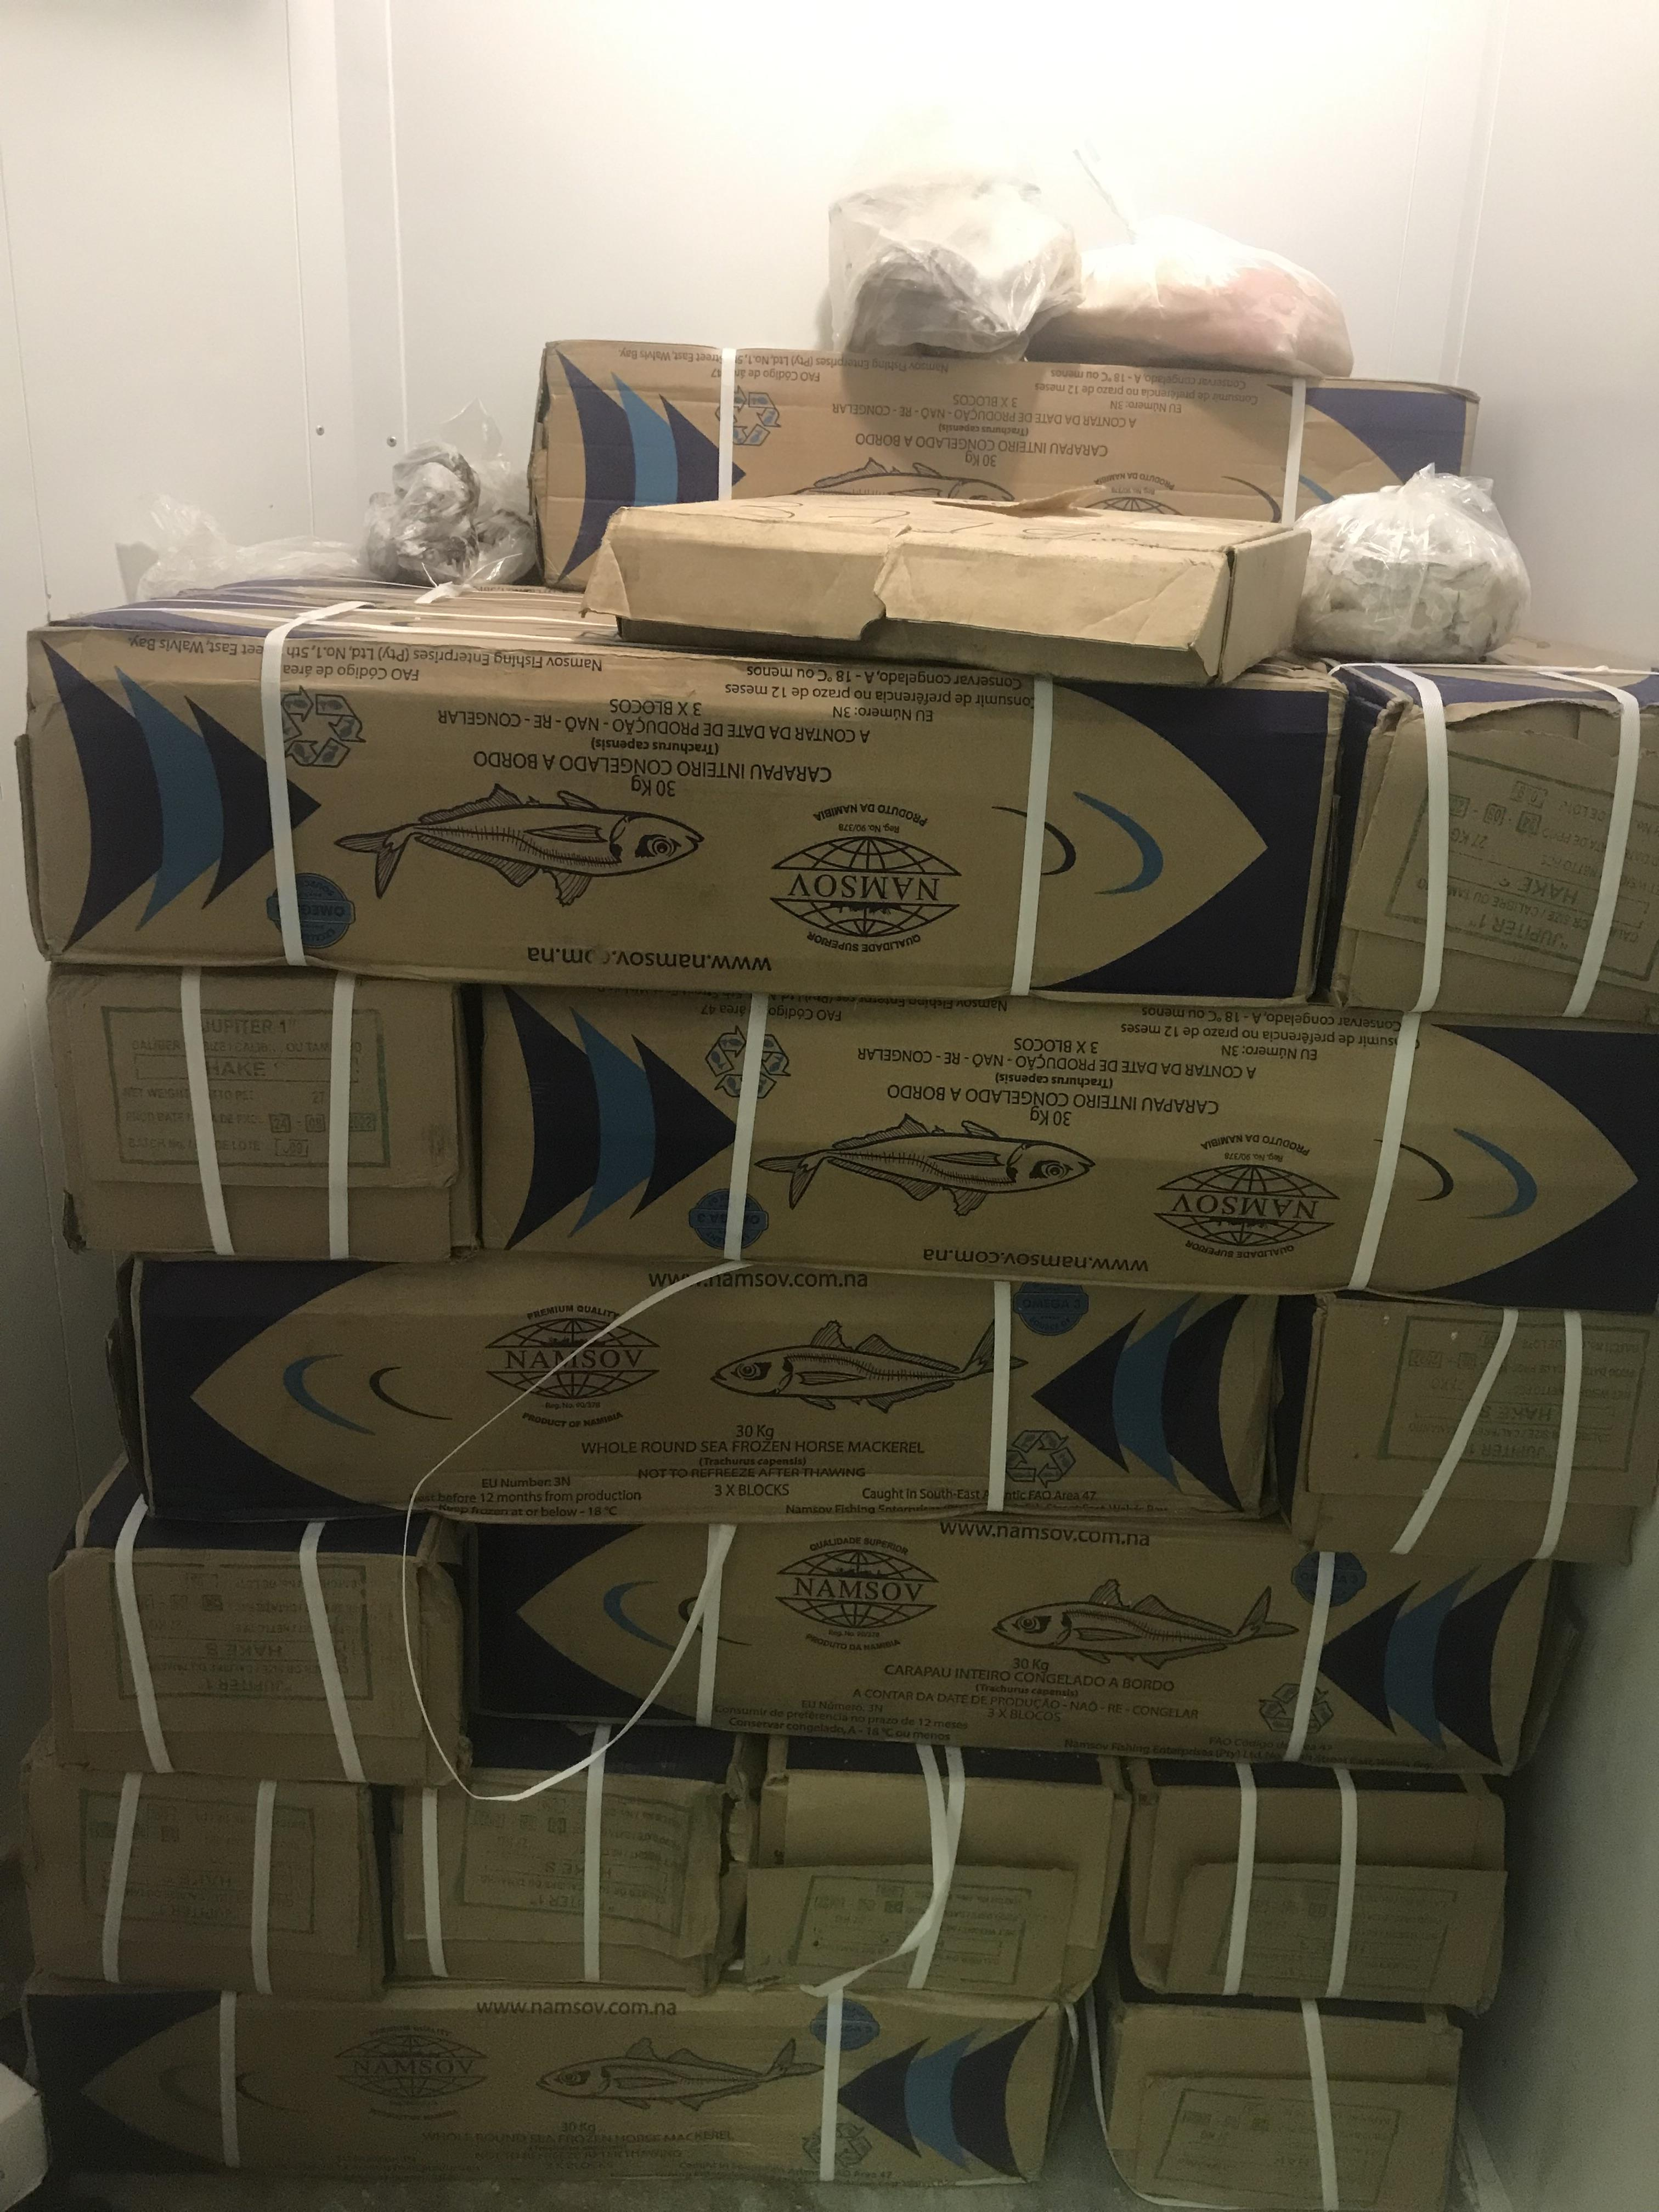
\includegraphics{images/feed/30kg2.jpg}

}

}

\subcaption{\label{fig-feed-thirty}30kg feed box}
\end{minipage}%
%
\begin{minipage}[t]{0.50\linewidth}

{\centering 

\raisebox{-\height}{

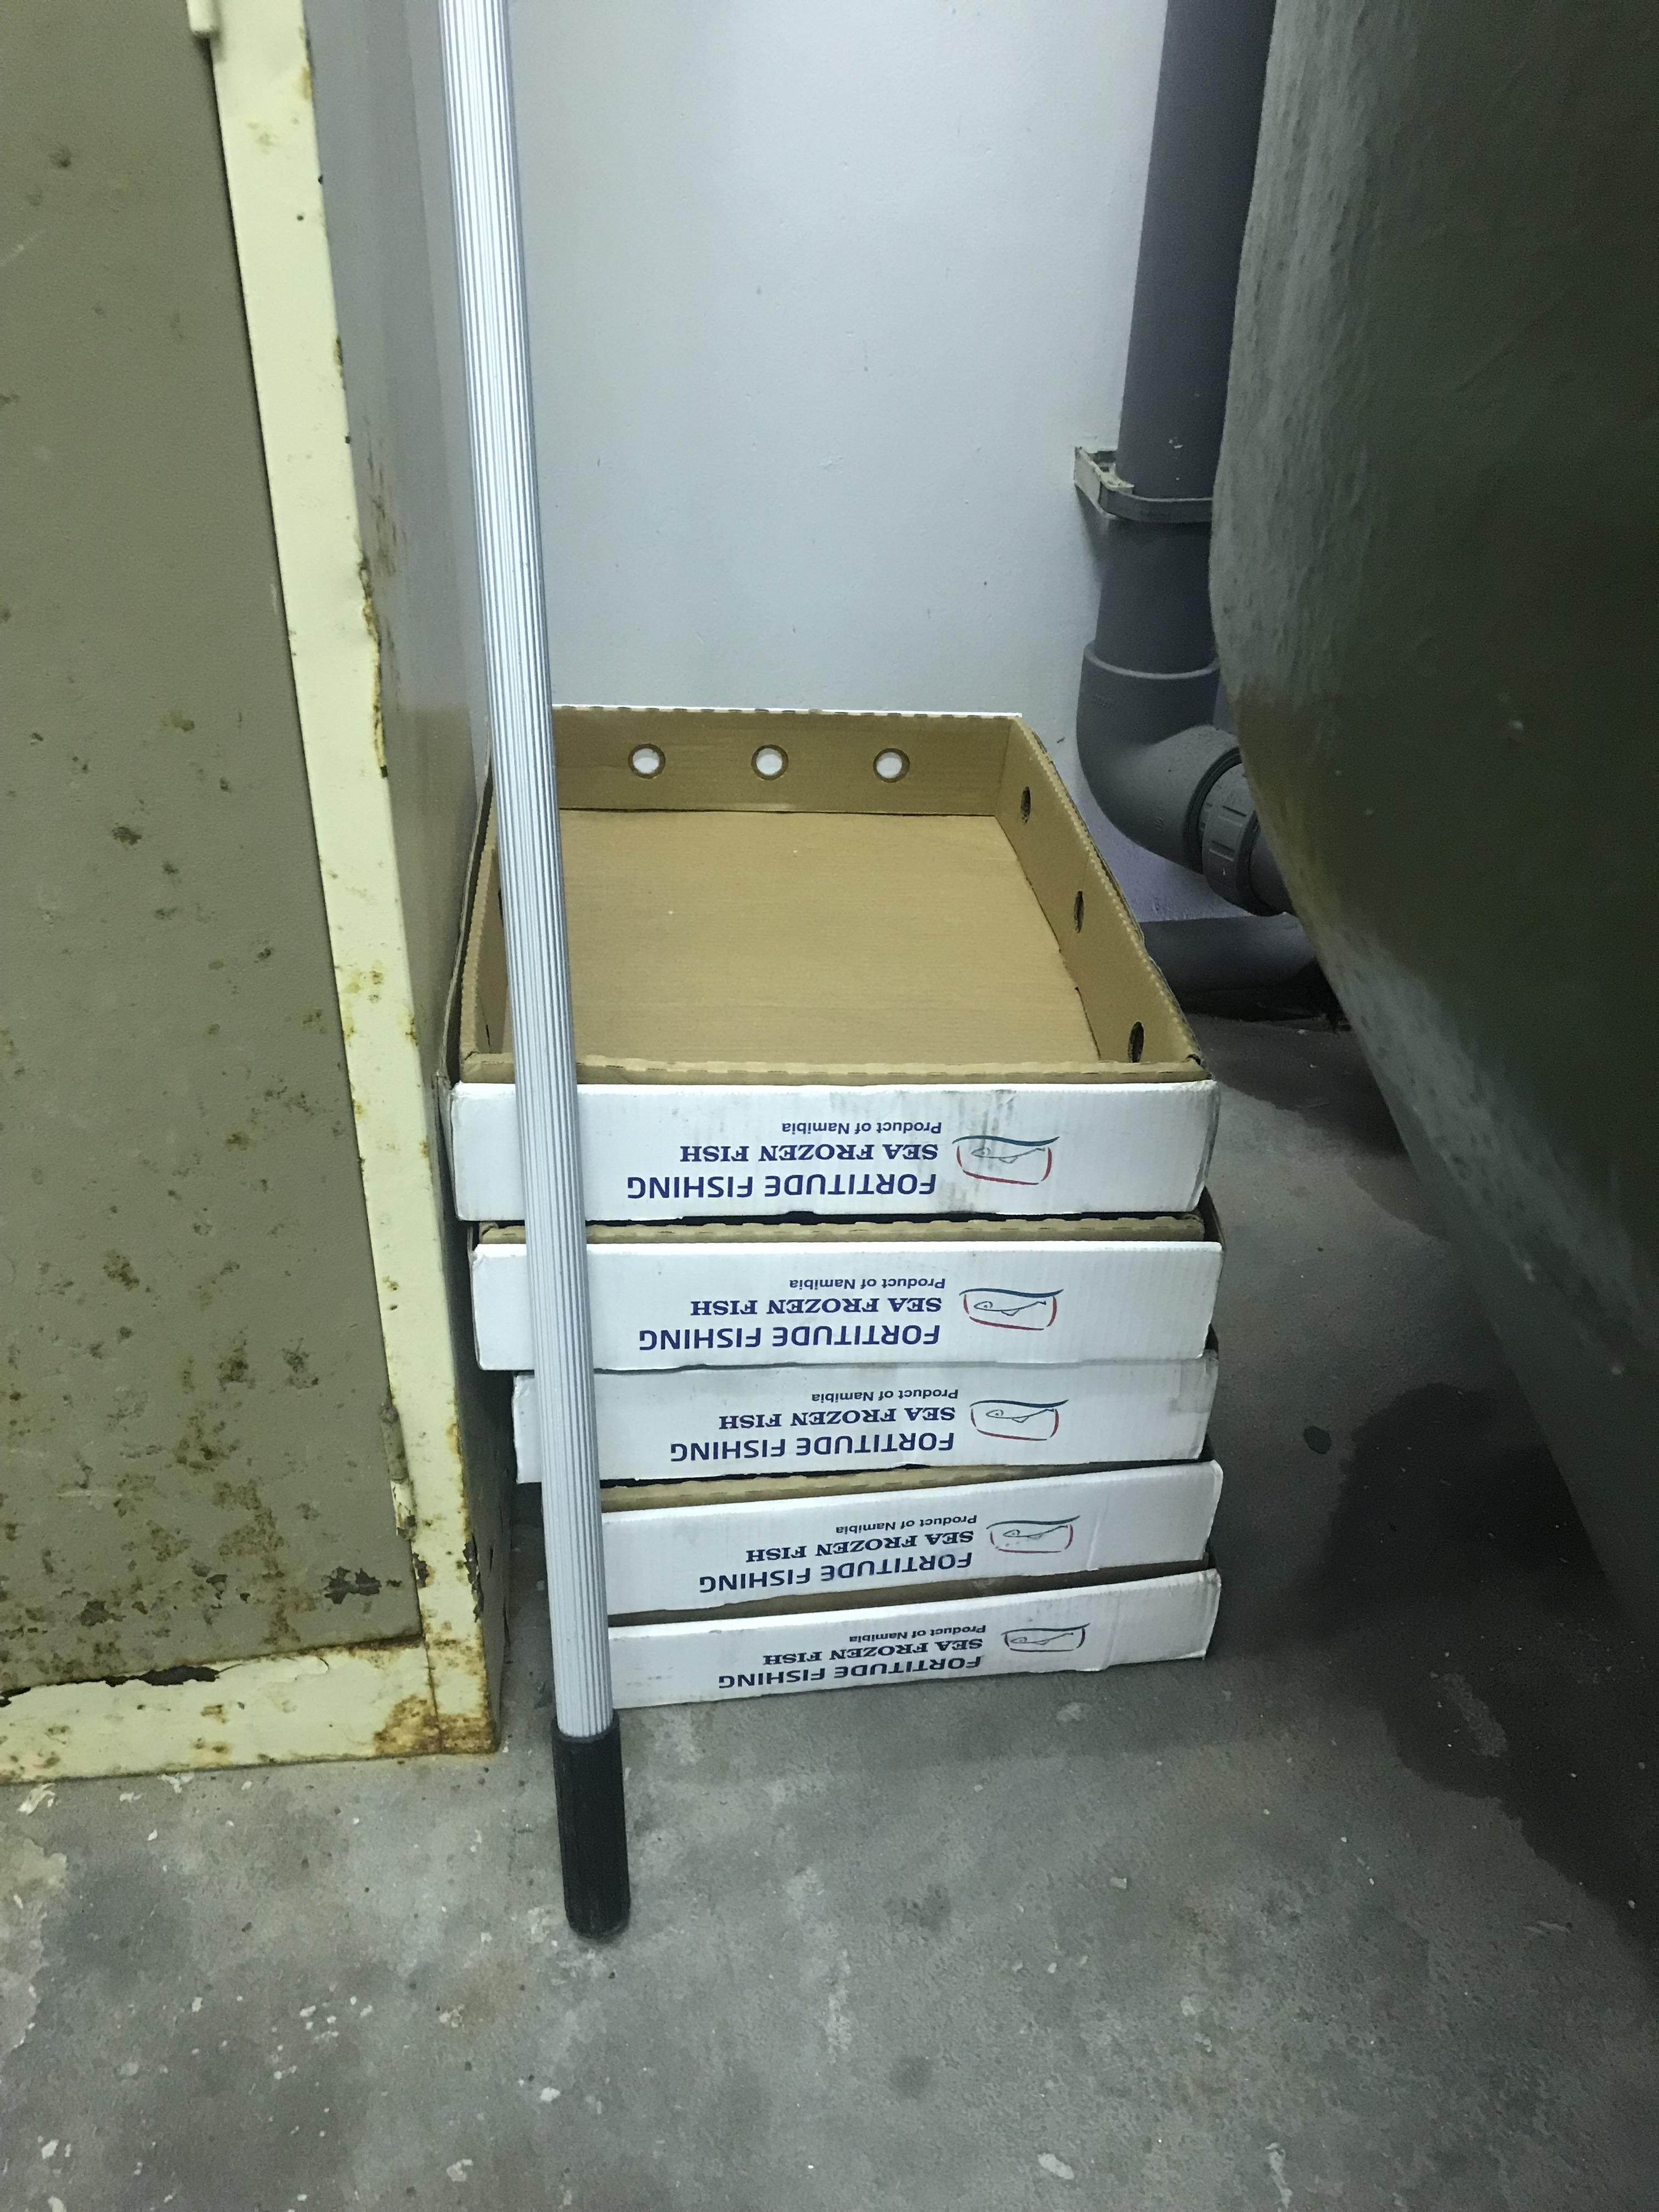
\includegraphics{images/feed/10kg2.jpg}

}

}

\subcaption{\label{fig-feed-ten}10kg feed box}
\end{minipage}%

\caption{\label{fig-feed-boxes}Image of the boxes used to package the
display animal's feed for transport and storage.}

\end{figure}

{Only one technical member of staff is required to collect the feed}.

\begin{enumerate}
\def\labelenumi{\arabic{enumi}.}
\tightlist
\item
  One of the supplier's operators will contact an Aquarium research
  technician, to provide an estimated time of arrival for the fresh feed
  at Namport.
\item
  Book the Cruiser for that day (Section ???).
\item
  Send the vehicle's licence plate number, as well as the name and ID
  number of the person collecting the feed, to the operator.
\item
  Make sure you have your Port access card (Section ???).
\item
  Drive to the Commercial harbour (Section ???) and park next to the
  freezer units at the wet docks (pic).
\end{enumerate}

\begin{itemize}
\tightlist
\item
  \emph{If there is no space available, you may have to stop at the car
  park found on the left hand side of the final entrance blockade,
  before the Commercial ship docks}.
\end{itemize}

\begin{enumerate}
\def\labelenumi{\arabic{enumi}.}
\setcounter{enumi}{5}
\tightlist
\item
  Report to the wet docks control office and give the operators the
  vehicle registration number.
\end{enumerate}

\begin{itemize}
\tightlist
\item
  \emph{The office can be found on the first floor, up the stairs to the
  right, immediately after entering the freezer unit}.
\item
  \emph{Ask one of the employees inside the freezer unit for directions,
  if you can not find the control office}.
\end{itemize}

\begin{enumerate}
\def\labelenumi{\arabic{enumi}.}
\setcounter{enumi}{6}
\tightlist
\item
  Go back down to the car
\item
  Wait for the order to be prepared and carted out to you.
\item
  Verify that the number of boxes brought out, match the number ordered.
\item
  Sign the receipt.
\item
  The employees stationed in that area will help load the boxes onto the
  back of the Cruiser.
\item
  Leave the Commercial harbour.
\item
  Visit the nearest service station and fill the cars tyres back up to
  2.4 bar.
\end{enumerate}

\begin{itemize}
\tightlist
\item
  \emph{The added weight might significantly decrease the tyre
  pressure}.\\
\end{itemize}

\begin{enumerate}
\def\labelenumi{\arabic{enumi}.}
\setcounter{enumi}{13}
\tightlist
\item
  Drive back to the Aquarium.
\end{enumerate}

\hypertarget{feed-packing}{%
\subsection{Feed packing}\label{feed-packing}}

\begin{enumerate}
\def\labelenumi{\arabic{enumi}.}
\setcounter{enumi}{14}
\tightlist
\item
  Park next to the rear entrance (Figure~\ref{fig-rear-entrance}).
\end{enumerate}

\begin{itemize}
\tightlist
\item
  \emph{Large double door entrance between the Quarantine area and the
  ocean}.
\end{itemize}

\begin{enumerate}
\def\labelenumi{\arabic{enumi}.}
\setcounter{enumi}{15}
\tightlist
\item
  Bring the Aquarium's trolley cart to the rear entrance
  (Figure~\ref{fig-trolley}).
\end{enumerate}

\begin{itemize}
\tightlist
\item
  \emph{The trolley is kept behind the two small, deep fridges in the
  Aquarium section underneath the Auditorium}.
\end{itemize}

\begin{figure}[H]

\begin{minipage}[t]{0.33\linewidth}

{\centering 

\raisebox{-\height}{

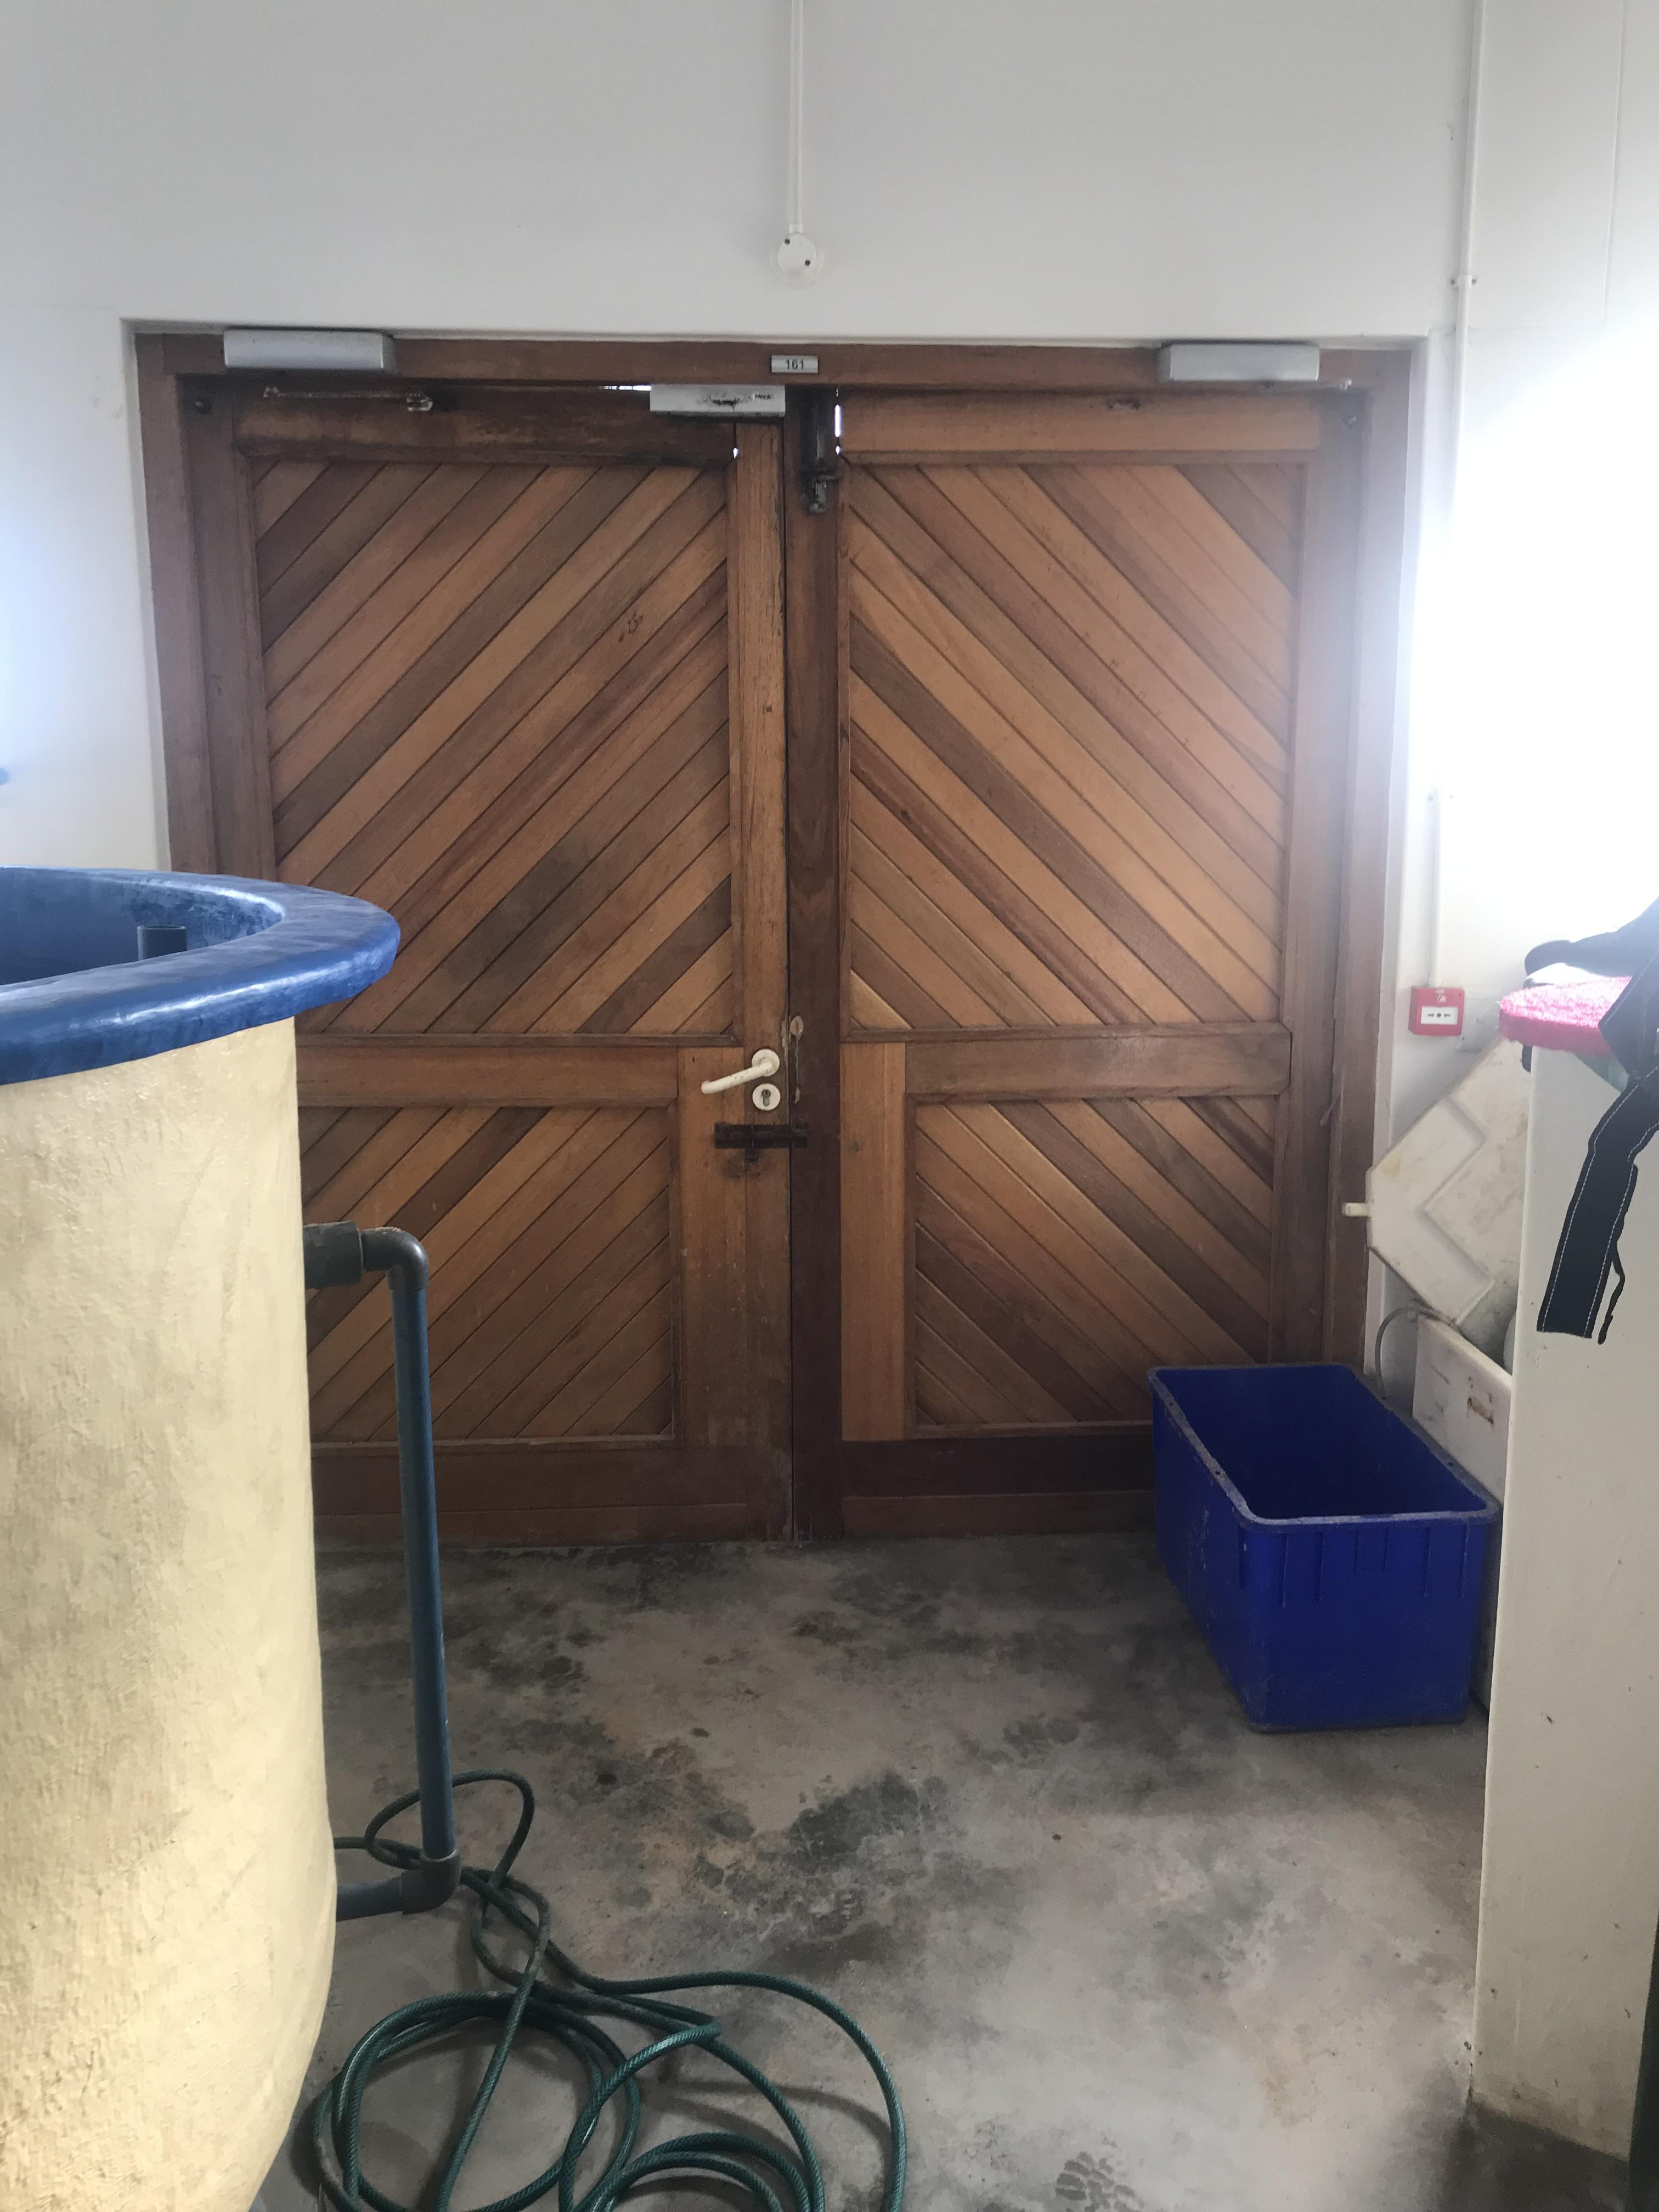
\includegraphics{images/feed/rear_entrance2.jpg}

}

}

\subcaption{\label{fig-rear-entrance}Rear entrance}
\end{minipage}%
%
\begin{minipage}[t]{0.33\linewidth}

{\centering 

\raisebox{-\height}{

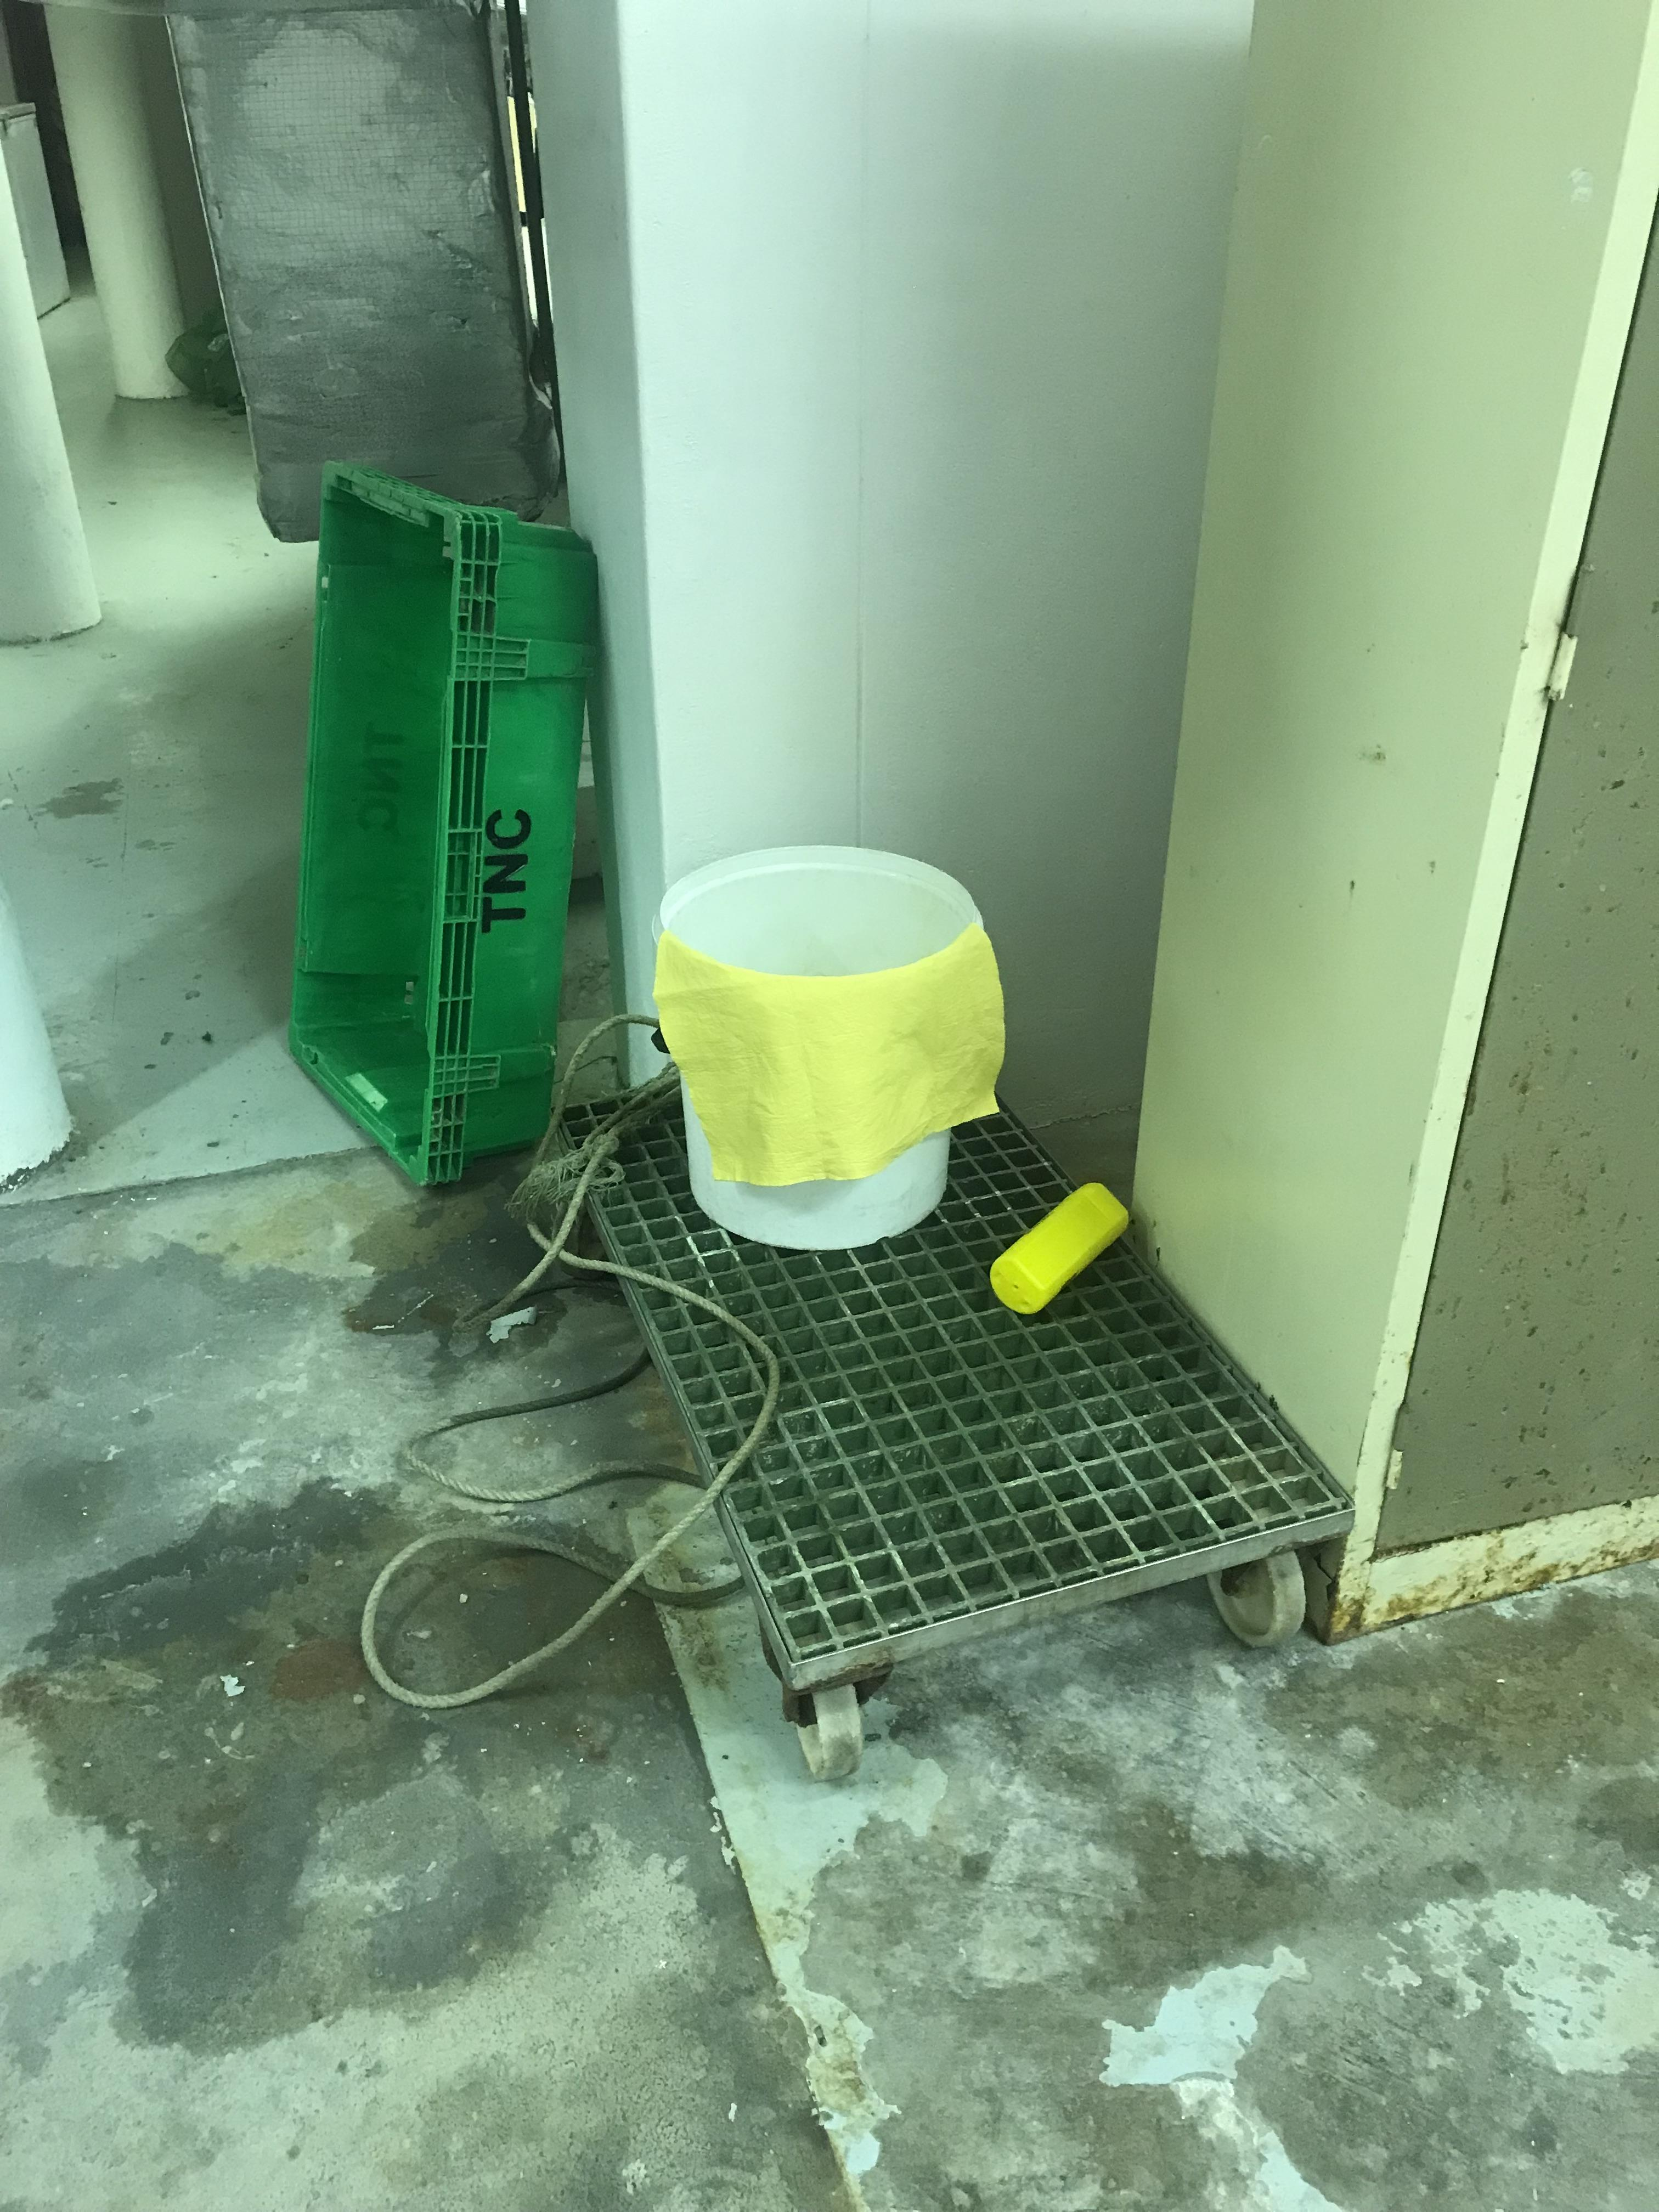
\includegraphics{images/feed/trolley2.jpg}

}

}

\subcaption{\label{fig-trolley}Trolley}
\end{minipage}%
%
\begin{minipage}[t]{0.33\linewidth}

{\centering 

\raisebox{-\height}{

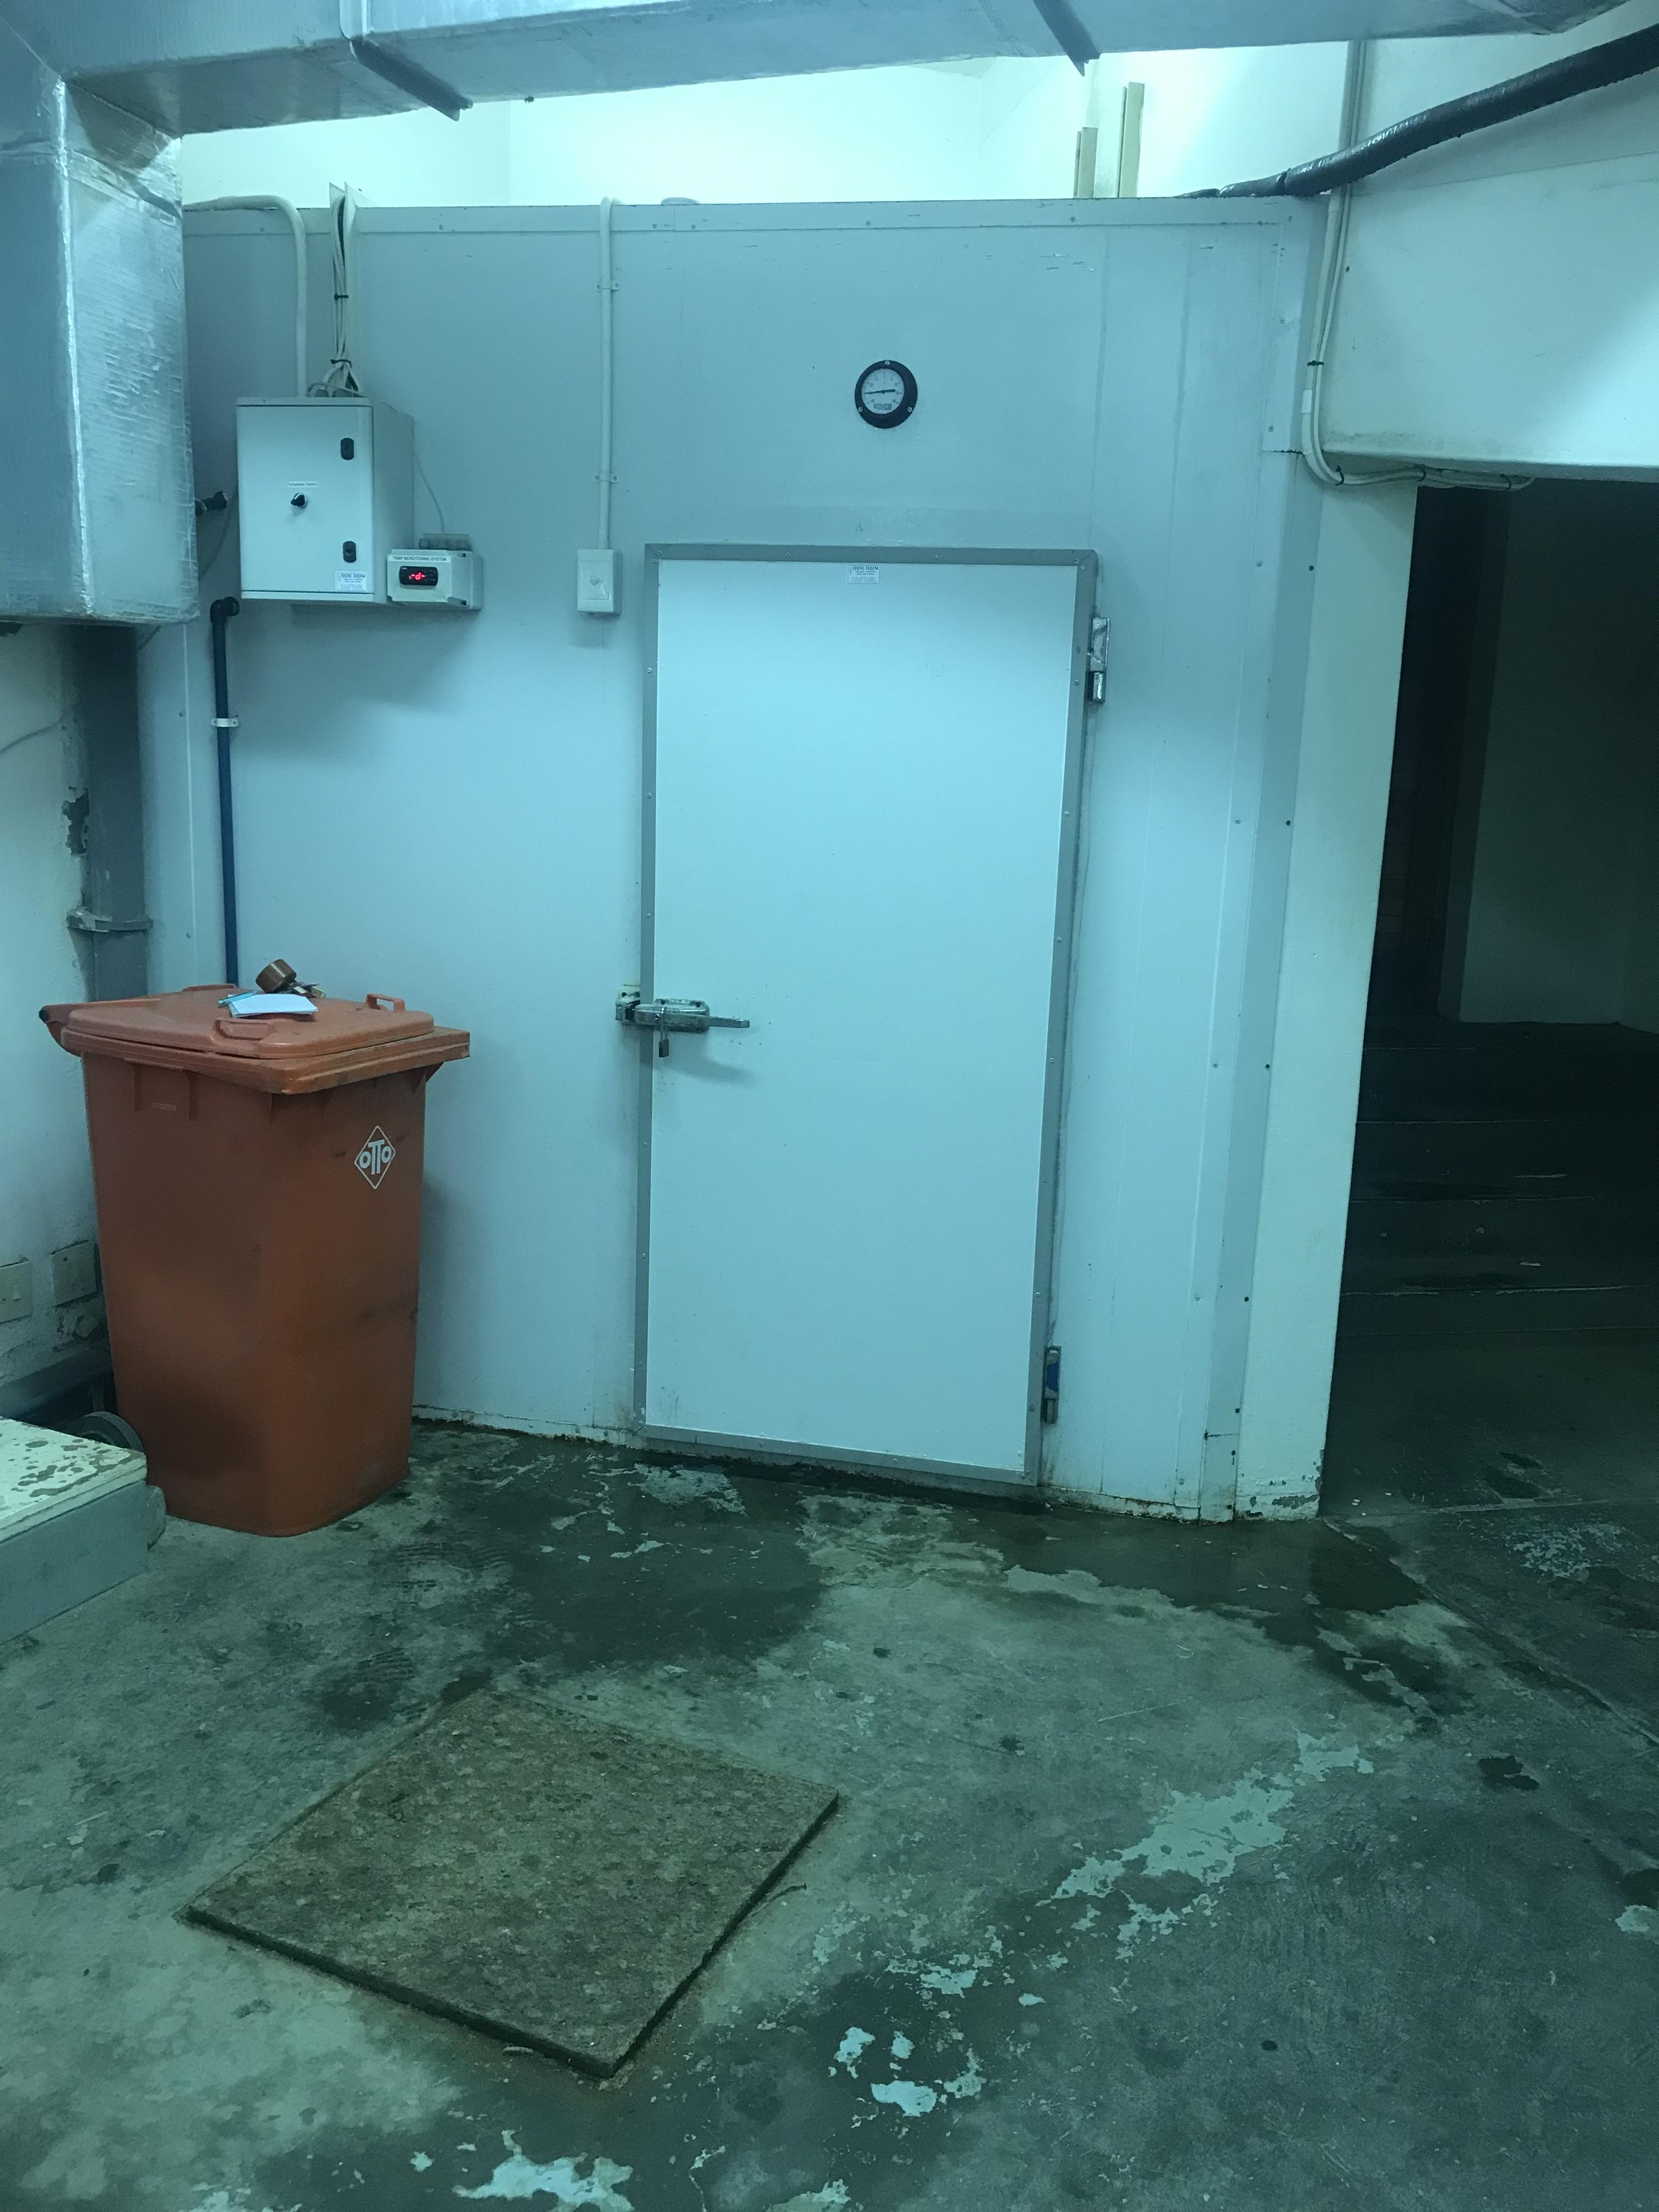
\includegraphics{images/feed/freezer2.jpg}

}

}

\subcaption{\label{fig-freezer}Freezer room}
\end{minipage}%

\caption{\label{fig-feed-packing}The different components required to
pack and store the feed within the Aquarium.}

\end{figure}

\begin{enumerate}
\def\labelenumi{\arabic{enumi}.}
\setcounter{enumi}{16}
\tightlist
\item
  Off load and pack a fraction of the total boxes onto the trolley.
\item
  Push the loaded trolley to the Aquarium Freezer
  (Figure~\ref{fig-freezer}).
\end{enumerate}

\begin{itemize}
\tightlist
\item
  \emph{Kept at approximately -25}\(^\circ\)C.
\end{itemize}

\begin{enumerate}
\def\labelenumi{\arabic{enumi}.}
\setcounter{enumi}{18}
\tightlist
\item
  Open the Freezer door and pack the boxes into the Freezer.
\end{enumerate}

\begin{itemize}
\item
  \emph{The freezer can be found on the Aquarium's ground floor,
  directly beneath the Feed room}.
\item
  \textbf{Repeat steps 16 - 19 until all the boxes of feed have been
  packed into the Freezer}.
\end{itemize}

\begin{enumerate}
\def\labelenumi{\arabic{enumi}.}
\setcounter{enumi}{19}
\tightlist
\item
  Indicate the amount and type of feed packed into the Freezer room on
  the Feed log sheet (Figure~\ref{fig-feed-logsheet}).
\end{enumerate}

\begin{itemize}
\tightlist
\item
  \emph{Kept in the Feed preparation room/``Feed room'' (Nr. 171),
  located to the left of the Main tanks top section on the Aquarium's
  top floor} (Figure~\ref{fig-feed-prep}).
\end{itemize}

\begin{figure}[H]

\begin{minipage}[t]{0.50\linewidth}

{\centering 

\raisebox{-\height}{

\includegraphics{images/feed/feed_log2.jpg}

}

}

\subcaption{\label{fig-feed-logsheet}Feed log sheet}
\end{minipage}%
%
\begin{minipage}[t]{0.50\linewidth}

{\centering 

\raisebox{-\height}{

\includegraphics{images/feed/feed_prep12.jpg}

}

}

\subcaption{\label{fig-feed-prep}Feed preparation room}
\end{minipage}%

\caption{\label{fig-feed-track}The Feed log sheet is kept in the Feed
room to help keep track of the amount of feed bought and used within the
Aquarium.}

\end{figure}

\begin{enumerate}
\def\labelenumi{\arabic{enumi}.}
\setcounter{enumi}{20}
\tightlist
\item
  Follow the vehicle return procedure (Section ???).
\end{enumerate}

\hypertarget{animal-feeding}{%
\section{Animal feeding}\label{animal-feeding}}

All animals kept in captivity have to be fed regularly to guarantee
their well being. In the Aquarium, this is done by either the Technical
assistants or by divers (volunteers or Aquarium technicians). Feeding
occurs everyday at 15h00, without exception.

\hypertarget{by-technical-assistants}{%
\subsection{By Technical assistants}\label{by-technical-assistants}}

The Technical assistants are responsible for preparing the feed
everyday. They also hand feed the animals from the tops of their
respective display tanks everyday except Tuesdays, Saturdays and
Sundays, if a diver is available.

{Only one Technical assistant is required to prepare the feed and to
feed the animals per day}.

\hypertarget{tools}{%
\subsubsection{Tools}\label{tools}}

\textbf{Most of the tools required can be found in the Feed room
(Section ???), in the Workshop (Nr. 162) or Diver preparation area
(Section ???)}.

These include:

\begin{itemize}
\tightlist
\item
  1 x Apron.
\item
  1 x Pair of rubber gloves.
\item
  1 x Wooden cutting board (Figure~\ref{fig-feed-bench}).
\item
  1 x Sharp knife.
\item
  2 x Round bucket.
\item
  1 x Modified divers bucket (Figure~\ref{fig-diver-bucket}).

  \begin{itemize}
  \tightlist
  \item
    \emph{Has a rubber cover, with a slit opening cut through its
    center, clamped over the top of the bucket and a rubber cover
    clamped over the bottom of the bucket}.
  \end{itemize}
\item
  1 x Feed log sheet.
\item
  1 x Knife sharpener.
\item
  1 x Large tray (Figure~\ref{fig-feed-tray}).

  \begin{itemize}
  \tightlist
  \item
    \emph{1m Long}.
  \end{itemize}
\end{itemize}

\begin{figure}[H]

\begin{minipage}[t]{0.33\linewidth}

{\centering 

\raisebox{-\height}{

\includegraphics{images/feed/feed_bench2.jpg}

}

}

\subcaption{\label{fig-feed-bench}Feed bench}
\end{minipage}%
%
\begin{minipage}[t]{0.33\linewidth}

{\centering 

\raisebox{-\height}{

\includegraphics{images/feed/round_bucket12.jpg}

}

}

\subcaption{\label{fig-feed-bucket}Feed bucket}
\end{minipage}%
%
\begin{minipage}[t]{0.33\linewidth}

{\centering 

\raisebox{-\height}{

\includegraphics{images/feed/large_tray2.jpg}

}

}

\subcaption{\label{fig-feed-tray}Feed tray}
\end{minipage}%

\caption{\label{fig-feed-tools}Some of the tools used to prepare the
feed and to feed the display animals.}

\end{figure}

\textbf{The number of different diving gear items used depends on the
number of divers on the day which, does not normally exceed two}.

\begin{itemize}
\tightlist
\item
  Air cylinders (10m\(l\))
\item
  Wet or dry suits (Figure~\ref{fig-wet-suit}).

  \begin{itemize}
  \tightlist
  \item
    \emph{Depends on the diver(s)}.
  \end{itemize}
\item
  Diving fins (Figure~\ref{fig-diving-fins}).

  \begin{itemize}
  \tightlist
  \item
    \emph{Referred to as Fins throughout}.
  \end{itemize}
\item
  Diving masks
\item
  Buoyancy control device (Figure~\ref{fig-bcd}).

  \begin{itemize}
  \tightlist
  \item
    \emph{Commonly called the BCD}.
  \end{itemize}
\item
  Nylon gloves
\item
  Diving regulators (Figure~\ref{fig-regulator}).

  \begin{itemize}
  \tightlist
  \item
    \emph{Referred to as the Regulator throughout}.
  \end{itemize}
\end{itemize}

\begin{figure}[H]

\begin{minipage}[t]{0.50\linewidth}

{\centering 

\raisebox{-\height}{

\includegraphics{images/dive_cylinders/wet_suit2.jpg}

}

}

\subcaption{\label{fig-wet-suit}Wet suit}
\end{minipage}%
%
\begin{minipage}[t]{0.50\linewidth}

{\centering 

\raisebox{-\height}{

\includegraphics{images/dive_cylinders/flippers2.jpg}

}

}

\subcaption{\label{fig-diving-fins}Diving fins}
\end{minipage}%
\newline
\begin{minipage}[t]{0.50\linewidth}

{\centering 

\raisebox{-\height}{

\includegraphics{images/dive_cylinders/regulator2.jpg}

}

}

\subcaption{\label{fig-regulator}Regulator}
\end{minipage}%
%
\begin{minipage}[t]{0.50\linewidth}

{\centering 

\raisebox{-\height}{

\includegraphics{images/dive_cylinders/BCD2.jpg}

}

}

\subcaption{\label{fig-bcd}bcd}
\end{minipage}%

\caption{\label{fig-dive-tools}Important pieces of diving attire
required to move and breathe comfortably under water.}

\end{figure}

\begin{itemize}
\tightlist
\item
  1 x Diver log sheet (Figure~\ref{fig-dive-log}).
\end{itemize}

\begin{figure}[H]

{\centering \includegraphics[width=0.5\textwidth,height=\textheight]{images/dive_cylinders/dive_log2.jpg}

}

\caption{\label{fig-dive-log}The diver log sheet, kept in the diver
preparation area.}

\end{figure}

\hypertarget{feed-preparation}{%
\subsubsection{Feed preparation}\label{feed-preparation}}

{See Section ??? for a description of the Feed boxes and their
contents}.

The animals are generally fed \(\pm\) 15kg (\(1\frac{1}{2}\) slabs from
the 30kg box or \(1\frac{1}{2}\) 10kg boxes) of food daily. However, the
daily amount can be adjusted according to the animals' voracity and the
Aquarium's stocking density. Only give the animals 10kg of feed if there
are large amounts of feed leftover from the previous day and 20kg if
there is consistently no food leftover, each day, for several days. The
animals are rarely fed 20kg in one day.

\begin{enumerate}
\def\labelenumi{\arabic{enumi}.}
\tightlist
\item
  Collect frozen feed from the Freezer room using the large tray.
\item
  Leave the frozen food in the Feed room to thaw.
\item
  Throw the used Feed box away if it is empty or put the box back in the
  Freezer if it is not.
\item
  The animal feed is generally allowed to thaw overnight (\(\pm\) 23hrs)
  or for \(\pm\) 6hrs on the day of feeding.
\end{enumerate}

\begin{itemize}
\tightlist
\item
  \emph{If the frozen feed is less than 6 weeks old, thaw overnight. If
  not, thaw on the same day to prevent unpleasant odors}.
\end{itemize}

\begin{enumerate}
\def\labelenumi{\arabic{enumi}.}
\setcounter{enumi}{4}
\tightlist
\item
  Put on appropriate feed preparation attire.
\end{enumerate}

\begin{itemize}
\tightlist
\item
  \emph{Apron and gloves}.
\end{itemize}

\begin{enumerate}
\def\labelenumi{\arabic{enumi}.}
\setcounter{enumi}{5}
\tightlist
\item
  Move the thawed fish to one of the round buckets.
\item
  Set the Feed preparation bench (Figure~\ref{fig-feed-bench}).
\end{enumerate}

\begin{itemize}
\tightlist
\item
  \emph{Get the Feed bucket (second round bucket or Diver's bucket),
  cutting board and knife ready}.
\end{itemize}

\begin{enumerate}
\def\labelenumi{\arabic{enumi}.}
\setcounter{enumi}{7}
\tightlist
\item
  Prepare the feed according to the display animal's size and the feed
  type.
\end{enumerate}

\begin{itemize}
\item
  \emph{Large animals e.g., Dusky kob, Garrick}

  \begin{itemize}
  \tightlist
  \item
    \emph{Small Pilchards/Horse mackerel can be fed whole}.
  \item
    \emph{The heads and backbones of large Hake pieces have to be
    removed before they are cut into medium sized pieces}.
  \end{itemize}
\item
  \emph{Medium sized animals e.g., Glajoen, Steenbra}.

  \begin{itemize}
  \tightlist
  \item
    \emph{The heads and backbones of all fish feed pieces have to be
    removed}.
  \item
    \emph{All feed has to be cut into small pieces}.
  \end{itemize}
\item
  \emph{Small animals e.g., Sea anemones, Klipfish, Shyshark}.

  \begin{itemize}
  \tightlist
  \item
    \emph{Feed is either crushed between the feeder's hands or small
    pieces are torn off (not done for Section ???)}.
  \end{itemize}
\item
  \emph{When the feed is cut into smaller pieces, they are all cut
  vertically along the lateral line, irrespective of feed type or size}.
\item
  \textbf{The knife can generally be sharpened every two weeks or if it
  becomes dull}.
\end{itemize}

\begin{enumerate}
\def\labelenumi{\arabic{enumi}.}
\setcounter{enumi}{8}
\tightlist
\item
  Put all prepared feed into the divers' bucket if a diver is available
  (Figure~\ref{fig-diver-bucket}).
\end{enumerate}

\begin{figure}[H]

{\centering \includegraphics[width=0.5\textwidth,height=\textheight]{images/feed/diver_bucket2.jpg}

}

\caption{\label{fig-diver-bucket}The second feed bucket, from which the
Aquarium's display animals are normally fed by divers}

\end{figure}

\hypertarget{feed-administration}{%
\subsubsection{Feed administration}\label{feed-administration}}

Two thirds of all prepared feed is given to the animals in the main tank
and the rest to the animals in the smaller tanks. The remaining feed is
distributed among the small tanks according to the number and size of
the animals inside them.

\begin{enumerate}
\def\labelenumi{\arabic{enumi}.}
\setcounter{enumi}{9}
\tightlist
\item
  Take the Feed bucket to the Main tank feeding spot, right outside the
  Feed room (Figure~\ref{fig-mt-border}).
\item
  Rest the Feed bucket on the boundary wall top
  (Figure~\ref{fig-mt-border}).
\end{enumerate}

\begin{figure}[H]

{\centering \includegraphics[width=0.5\textwidth,height=\textheight]{images/feed/mt_border2.jpg}

}

\caption{\label{fig-mt-border}The Main tank boundary wall, which acts as
the Aquarium staffs' primary feeding location.}

\end{figure}

\begin{enumerate}
\def\labelenumi{\arabic{enumi}.}
\setcounter{enumi}{11}
\tightlist
\item
  Throw handfuls of food across the entire water surface at short 1-2
  minute intervals.
\item
  Take the Feed bucket to the Pelagic tank
  (Figure~\ref{fig-pelagic-tank}), found in the Aquarium's main display
  area on the ground floor.
\end{enumerate}

\begin{itemize}
\tightlist
\item
  \emph{Circular tank with South African mullet fish}.
\end{itemize}

\begin{enumerate}
\def\labelenumi{\arabic{enumi}.}
\setcounter{enumi}{13}
\tightlist
\item
  Put the Feed bucket on the floor.
\item
  Open the small wooden hatch (Figure~\ref{fig-pelagic-hatch}), found at
  the top of the Pelagic tank, and throw the food in.
\end{enumerate}

\begin{figure}[H]

\begin{minipage}[t]{0.50\linewidth}

{\centering 

\raisebox{-\height}{

\includegraphics{images/feed/pelagic2.jpg}

}

}

\subcaption{\label{fig-pelagic-tank}Pelagic tank}
\end{minipage}%
%
\begin{minipage}[t]{0.50\linewidth}

{\centering 

\raisebox{-\height}{

\includegraphics{images/feed/pelagic_hatch2.jpg}

}

}

\subcaption{\label{fig-pelagic-hatch}Pelagic hatch}
\end{minipage}%

\caption{\label{fig-pelagic}The Pelagic tank and it's wooden hatch,
built into the tank's wooden frame near the Aquarium first floor
ceiling.}

\end{figure}

\begin{enumerate}
\def\labelenumi{\arabic{enumi}.}
\setcounter{enumi}{15}
\tightlist
\item
  Take the feed to the Touch pool (Figure~\ref{fig-touch-pool}), in
  front of the receptionist's desk.
\end{enumerate}

\begin{itemize}
\tightlist
\item
  \emph{Short tank with the Ray sharks}.
\end{itemize}

\begin{figure}[H]

{\centering \includegraphics[width=0.5\textwidth,height=\textheight]{images/feed/touch_pool2.jpg}

}

\caption{\label{fig-touch-pool}The Aquarium touch pool houses skates and
rays.}

\end{figure}

\begin{enumerate}
\def\labelenumi{\arabic{enumi}.}
\setcounter{enumi}{16}
\tightlist
\item
  Rest the Feed bucket on the boundary wall top.
\item
  Throw some of the feed into the tank.
\item
  Take the Feed bucket to the back of the remaining small display tanks
  (Figure~\ref{fig-st-back}), behind the CFRT's office.
\item
  Throw feed into these tanks, sequentially, from right to left.
\end{enumerate}

\begin{itemize}
\tightlist
\item
  \emph{Rinse hands with water inside the Sea anemone tank after
  crushing some feed between your fingers (Section ???)}.
\item
  \emph{Only small torn off pieces of feed (Section ???) should be
  thrown into the Shyshark and Klipfish tank}.
\end{itemize}

\begin{figure}[H]

\begin{minipage}[t]{0.50\linewidth}

{\centering 

\raisebox{-\height}{

\includegraphics{images/feed/st_front2.jpg}

}

}

\subcaption{\label{fig-st-front}Front end}
\end{minipage}%
%
\begin{minipage}[t]{0.50\linewidth}

{\centering 

\raisebox{-\height}{

\includegraphics{images/feed/st_back2.jpg}

}

}

\subcaption{\label{fig-st-back}Back end}
\end{minipage}%

\caption{\label{fig-small-tanks}The front, viewable end and the back,
service end of the Aquarium's small tanks, found behind the
Receptionist's desk.}

\end{figure}

\begin{enumerate}
\def\labelenumi{\arabic{enumi}.}
\setcounter{enumi}{20}
\tightlist
\item
  Take the empty Feed bucket back up to the Feed room.
\item
  Record the amount and type of feed used in the Feed log sheet
  (Figure~\ref{fig-feed-logsheet}).
\item
  Clean and pack all used tools, and Feed preparation attire away.
\end{enumerate}

\hypertarget{by-divers}{%
\subsection{By divers}\label{by-divers}}

If the Research technicians have valid diver's licenses or if
recreational divers are available to assist with feeding, feeding by
diving is generally done on the days specified in Section ???.

\hypertarget{diver-preparation}{%
\subsubsection{Diver preparation}\label{diver-preparation}}

The divers always prepare for diving sessions in the Diver preparation
area (Section ???).

\begin{enumerate}
\def\labelenumi{\arabic{enumi}.}
\tightlist
\item
  Put the diving suit on.
\item
  Conduct a quick inspection of the Air cylinders (Section ???) to
  ensure that they are not significantly damaged.
\end{enumerate}

\begin{itemize}
\tightlist
\item
  \emph{Cylinder condition is usually determined during Air cylinder
  testing (Section ???) but, between cylinder condition should be
  assessed routinely (between each diving session) for safety reasons}.
\item
  \emph{Make sure the Cylinders air outlet o-ring is clear of any
  defects}.
\end{itemize}

\begin{enumerate}
\def\labelenumi{\arabic{enumi}.}
\setcounter{enumi}{2}
\tightlist
\item
  Secure the BCD to the Air cylinder.
\end{enumerate}

\begin{itemize}
\tightlist
\item
  \emph{The tank's outlet valve and the BCD neck should be approximately
  aligned}.
\end{itemize}

\begin{enumerate}
\def\labelenumi{\arabic{enumi}.}
\setcounter{enumi}{3}
\tightlist
\item
  Make sure the Cylinder's outlet valve is closed.
\end{enumerate}

\begin{itemize}
\tightlist
\item
  \emph{Clockwise to close}.
\end{itemize}

\begin{enumerate}
\def\labelenumi{\arabic{enumi}.}
\setcounter{enumi}{4}
\tightlist
\item
  Remove the Regulator's dust cap (Figure~\ref{fig-dust-cap}).
\end{enumerate}

\begin{itemize}
\tightlist
\item
  \emph{In place to protect the Regulator's filter from dust when it is
  not in use}.
\end{itemize}

\begin{enumerate}
\def\labelenumi{\arabic{enumi}.}
\setcounter{enumi}{5}
\tightlist
\item
  Fasten the Regulator to the Cylinder's air outlet.
\end{enumerate}

\begin{itemize}
\tightlist
\item
  \emph{The Regulator mouth piece should be on the right hand side}.
\item
  \emph{Tighten the Regulator's yoke screw with your hands}
  (Figure~\ref{fig-yoke-valve}).
\end{itemize}

\begin{figure}[H]

\begin{minipage}[t]{0.50\linewidth}

{\centering 

\raisebox{-\height}{

\includegraphics{images/dive_cylinders/dust_cap2.jpg}

}

}

\subcaption{\label{fig-dust-cap}Dust cap}
\end{minipage}%
%
\begin{minipage}[t]{0.50\linewidth}

{\centering 

\raisebox{-\height}{

\includegraphics{images/dive_cylinders/yoke_valve2.jpg}

}

}

\subcaption{\label{fig-yoke-valve}Yoke valve}
\end{minipage}%

\caption{\label{fig-dive-prep}Picture displaying some of the diving gear
components that need to be inspected during diver preparation.}

\end{figure}

\begin{enumerate}
\def\labelenumi{\arabic{enumi}.}
\setcounter{enumi}{6}
\tightlist
\item
  Connect the Low pressure inflator to the BCD.
\item
  Secure the Alternate mouth piece to the BCD vest.
\item
  Inspect the Cylinder's air pressure to determine if there is enough
  air.
\end{enumerate}

\begin{itemize}
\tightlist
\item
  \emph{Open the Outlet valve slowly at first and then completely open
  it}.

  \begin{itemize}
  \tightlist
  \item
    \emph{One turn anti-clockwise after opening it completely}.
  \end{itemize}
\item
  \emph{The Cylinder's manometer should have a reading of} \(\pm\) 200
  bar.
\end{itemize}

\begin{enumerate}
\def\labelenumi{\arabic{enumi}.}
\setcounter{enumi}{9}
\tightlist
\item
  Put the BCD on, along with its assembled components.
\item
  Put on the gloves (Figure~\ref{fig-dive-gloves}).
\item
  Carry the Fins to the Main tank feeding spot (Section ???).
\end{enumerate}

\begin{figure}[H]

{\centering \includegraphics[width=0.5\textwidth,height=\textheight]{images/dive_cylinders/dive_gloves2.jpg}

}

\caption{\label{fig-dive-gloves}The nylon gloves worn by the divers
during diving sessions.}

\end{figure}

\hypertarget{feed-preparation-1}{%
\subsubsection{Feed preparation}\label{feed-preparation-1}}

\textbf{See Section ???}

\hypertarget{feed-administration-1}{%
\subsubsection{Feed administration}\label{feed-administration-1}}

The Feed is distributed among the Aquarium display tanks in the same
proportions described in Section ???. The divers only feed the animals
in the Main tank, whereas animals in the remaining tanks are fed by the
TAs (Section ???).

\begin{enumerate}
\def\labelenumi{\arabic{enumi}.}
\setcounter{enumi}{22}
\tightlist
\item
  Take the filled Diver bucket to the Main tank.
\item
  Rest the Diver bucket on the boundary wall top.
\item
  Put the Fins on.
\item
  Get into the water
\item
  Put on the mouth piece and Diving mask.
\item
  Grab the bucket and dive to the bottom of the Main tank.
\end{enumerate}

\begin{itemize}
\tightlist
\item
  \emph{Control your buoyancy by inflating/deflating the BCD}.
\end{itemize}

\begin{enumerate}
\def\labelenumi{\arabic{enumi}.}
\setcounter{enumi}{28}
\tightlist
\item
  The divers feed the animals in one of two main ways. By:
\end{enumerate}

\begin{itemize}
\tightlist
\item
  \emph{Letting the animals take the food directly from their hands}.
\item
  \emph{Throwing the food right in front of or above themselves and
  letting the animals take the food from the water column}.

  \begin{itemize}
  \tightlist
  \item
    \emph{Recommended when the Dusky kob approach}.
  \end{itemize}
\end{itemize}

\begin{enumerate}
\def\labelenumi{\arabic{enumi}.}
\setcounter{enumi}{29}
\tightlist
\item
  Resurface once the feeding session in the Main tank is complete.
\end{enumerate}

\begin{itemize}
\tightlist
\item
  \emph{Inflate the BCD}.
\end{itemize}

\hypertarget{end-diving-session}{%
\subsubsection{End diving session}\label{end-diving-session}}

\begin{enumerate}
\def\labelenumi{\arabic{enumi}.}
\setcounter{enumi}{29}
\tightlist
\item
  Remove the mouth piece.
\item
  Rest the Diver bucket on the boundary wall top.
\item
  Take the Fins off and throw them out of the Main tank.
\item
  Climb out of the Main tank.
\item
  Take off the Mask.
\item
  Take the Diver's bucket back to the Feed room.
\item
  One of the TAs will complete the procedure described in Steps 21-23,
  Section ???.
\item
  Carry the Fins back down to the Diver preparation area.
\item
  Remove the gloves.
\item
  Take the Alternate mouth piece off the BCD.
\item
  Remove the BCD.
\item
  Disconnect the Low pressure inflator from the BCD.
\item
  Close the Cylinder's outlet valve.
\item
  Loosen the Regulator Yoke screw.
\item
  Take the Regulator off the Cylinder's air outlet.
\item
  Decouple the Cylinder from the BCD.
\item
  Pack all diving gear away neatly, in their respective storage spaces.
\end{enumerate}

\begin{itemize}
\tightlist
\item
  \textbf{The diver can take a warm shower at this stage, if they feel
  the need}.
\end{itemize}

\begin{enumerate}
\def\labelenumi{\arabic{enumi}.}
\setcounter{enumi}{45}
\tightlist
\item
  Record all details of the dive in the Diver log sheet
  (Figure~\ref{fig-dive-log}).
\end{enumerate}



\end{document}
